% -------------------------------------------
% linux
% FileHistories: 109829 
% ProjectVersions: 997486 
% FileVersions: 2335535 
% First Version: 
% 	 hash: 1da177e4c3f41524e886b7f1b8a0c1fc7321cac2 
% 	 date: Sun Apr 17 00:20:36 CEST 2005 
% Last Version: 
% 	 hash: 705191b03d507744c7e097f78d583621c14988ac 
% 	 date: Tue Apr 19 19:19:02 CEST 2022 
% Diff: {DAYS=6, HOURS=18, MINUTES=58, SECONDS=26, MILLISECONDS=0, MICROSECONDS=0, NANOSECONDS=0, YEARS=17}
% -------------------------------------------
% elastic
% FileHistories: 41043 
% ProjectVersions: 34842 
% FileVersions: 326543 
% First Version: 
% 	 hash: 222b36344f0939f12cf54358e7047239cd398463 
% 	 date: Fri Jun 28 09:22:10 CEST 2013 
% Last Version: 
% 	 hash: 2cdffdce2ab35416bd5b1b7ea889cd0dede5b6c8 
% 	 date: Thu Apr 14 14:36:03 CEST 2022 
% Diff: {DAYS=292, HOURS=5, MINUTES=13, SECONDS=53, MILLISECONDS=0, MICROSECONDS=0, NANOSECONDS=0, YEARS=8}
% -------------------------------------------
% libreoffice
% FileHistories: 213791 
% ProjectVersions: 367996 
% FileVersions: 1924183 
% First Version: 
% 	 hash: 5acbb755f3f8dedf51904b711ff78f5e1aa498cf 
% 	 date: Thu Mar 07 16:45:23 CET 2002 
% Last Version: 
% 	 hash: 634f13a722dc68b7a2df7518880ce4f9d5d89f19 
% 	 date: Sat Jun 18 16:10:53 CEST 2022 
% Diff: {DAYS=107, HOURS=22, MINUTES=25, SECONDS=30, MILLISECONDS=0, MICROSECONDS=0, NANOSECONDS=0, YEARS=20}
% -------------------------------------------
% JetUML
% FileHistories: 795 
% ProjectVersions: 2013 
% FileVersions: 10176 
% First Version: 
% 	 hash: f232d9e7386cb9a6cca62600137cd10730a6a388 
% 	 date: Wed Jan 07 19:59:09 CET 2015 
% Last Version: 
% 	 hash: e47976ca608b40521a5410b0b697d5aae620858d 
% 	 date: Thu May 12 19:32:31 CEST 2022 
% Diff: {DAYS=126, HOURS=22, MINUTES=33, SECONDS=22, MILLISECONDS=0, MICROSECONDS=0, NANOSECONDS=0, YEARS=7}
% -------------------------------------------
% argouml
% FileHistories: 11129 
% ProjectVersions: 16672 
% FileVersions: 91667 
% First Version: 
% 	 hash: 6ef818a48b453627fd282971f3f9a28e28f54390 
% 	 date: Mon Jan 26 23:19:17 CET 1998 
% Last Version: 
% 	 hash: 3ddc7f94d83c4e2f439ca6fc0fe787616a1900a9 
% 	 date: Sat May 29 23:18:44 CEST 2021 
% Diff: {DAYS=128, HOURS=22, MINUTES=59, SECONDS=27, MILLISECONDS=0, MICROSECONDS=0, NANOSECONDS=0, YEARS=23}



\chapter[Case studies]{Case studies}
\graphicspath{ {images/casestudies} }

This chapter presents an actual case use scenario of SYN applied to open-source software systems. 
We use SYN to analyze the evolution of JetUML, the test project on which we relied during the development phase of the platform, ArgoUML, Elasticsearch, and Linux. 
\autoref{tab:casestudies} describes the characteristics of these systems.

\begin{table}[ht]
    \centering
    \begin{tabular}{lcrr} 
        \hline
        {\bf Name} & {\bf First Analyzed Commit} & {\bf Last Analyzed Commit} & {\bf \# of commits}\\ 
        \hline
        JetUML & 07 Jan 2015 & 12 May 2022 & 2'152 \\ 
        ArgoUML & 26 Jan 1998 & 29 May 2021 & 16'672  \\
        Elasticsearch & 28 Jun 2013 & 14 Apr 2022 & 34'842  \\
        Libreoffice & 07 Mar 2002 & 18 Jun 2022 & 367'996  \\
        Linux & 17 Apr 2005 & 19 Apr 2022 & 997'486  
    \end{tabular}
    \caption{List of analyzed projects}
    \label{tab:casestudies}
\end{table}

\bigbreak
There are many possible combinations to create a view specification; we explored them on all the projects. 
Each visualization has its purpose. For example, we can create a visualization to see the evolution of only Java files, or we can create a visualization to see how the system evolved every day. 
However, not all the combinations might have sense. For example, if we chose a timestamp grouping strategy, the time window must be chosen conscientiously. 
A comprehensive time window might hide some exciting aspects of the analysis. In contrast, a short time window could cause a massive number of AnimationFrames, undermining the understandability of the view. 
\bigbreak
A constant factor of all our visualization is the choice not to show deleted entities, the adoption of a LinearBucketValueStrategy for the mapper with a maximum height of 20, and finally, to display files that do not have the selected metric on the visualization. 
These properties are set as follow:
\begin{itemize}
    \item \texttt{showUnmappedEntities}: true.
    \item \texttt{mapperStrategy}: LinearBucketValueStrategy.
    \item \texttt{mapperStrategyOptions}: max height of 20.
    \item \texttt{showDeletedEntities}: false.
\end{itemize}
We made this choice because, during the development process, we have seen that the LinearBucketValueStrategy works better than other strategies. Of course, it needs a maximum height because otherwise, the gap between entities is too broad. Therefore set this value to 20. Moreover, we believe that hiding the deleted entities is the most intuitive thing for the user. On the other hand, hiding the unmapped entities might be misleading in some visualization. For this reason, we preferred to keep them. 


% -------------------------------------------
% JetUML
% FileHistories: 795 
% ProjectVersions: 2013 
% FileVersions: 10176 
% First Version: 
% 	 hash: f232d9e7386cb9a6cca62600137cd10730a6a388 
% 	 date: Wed Jan 07 19:59:09 CET 2015 
% Last Version: 
% 	 hash: e47976ca608b40521a5410b0b697d5aae620858d 
% 	 date: Thu May 12 19:32:31 CEST 2022 
% Diff: {DAYS=126, HOURS=22, MINUTES=33, SECONDS=22, MILLISECONDS=0, MICROSECONDS=0, NANOSECONDS=0, YEARS=7}
% ------------------------------------------- 

\section{JetUML 1}
This section analyzes JetUML, an open-source desktop application to work with UML diagrams. It is hosted on GitHub at the following address \url{https://github.com/prmr/JetUML}. Data collected in our analysis shows that the repository's history starts on the 07 Jan 2015 and ends 2'013 commits later on the 12 May 2022. The system's lifetime is over seven years of activity; within this range, we detected 795 FileHistories and more than 10K FileVersions.

%\subsection{View 1}
\begin{figure}[t]
    \begin{subfigure}{0.42\textwidth}
        
\includegraphics[width=\linewidth]{JetUML_V0E0.png}
        \caption{Commit that involved few entities} \label{fig:JetUML_V0E0}
    \end{subfigure}
    \hspace*{\fill}
    \begin{subfigure}{0.42\textwidth}
        
\includegraphics[width=\linewidth]{JetUML_V0E1.png}
        \caption{Commit that involved numerous entities} \label{fig:JetUML_V0E1}
    \end{subfigure}
    \caption{Comparison of commits with a low and an high activity} 
    \label{fig:JetUML_V0E0}
\end{figure}

\textbf{Goal of this visualization} Visualize the entire repository commit by commit to see how the repository evolved and understand commits with high activity. 
To highlight them, we use a one-commit aging strategy, maximum age of two. In other words, files modified by the displayed commit have an age of zero, whereas others have an age of one.
Consequently, all the files not included in the depicted commit are painted with the base color (gray by default). 

Figure \ref{fig:JetUML_V0E0} shows the graphical difference between commits that modified a few entities and commits that changed numerous entities. To identify highly active commits, we focused on commits that involved a considerable amount of files part of the repository at that time.

The view specification of this visualization is the following
\begin{itemize}
    \item \texttt{versionGroupingStrategy}: commit.
    \item \texttt{versionGroupingChunkSize}: 1. 
    \item \texttt{colorPalette}: default.
    \item \texttt{agingGroupingStrategy}: commit.
    \item \texttt{agingStepSize}: 1.
    \item \texttt{agingSteps}: 2 steps. 
    \item \texttt{mapperMetricName}: SIZE. 
    \item \texttt{fileTypeShape}: all boxes.
    \item \texttt{fileTypeOpacity}: all 1. 
\end{itemize}

\textbf{Results}

\begin{figure}[ht]
    \begin{subfigure}{0.42\textwidth}
        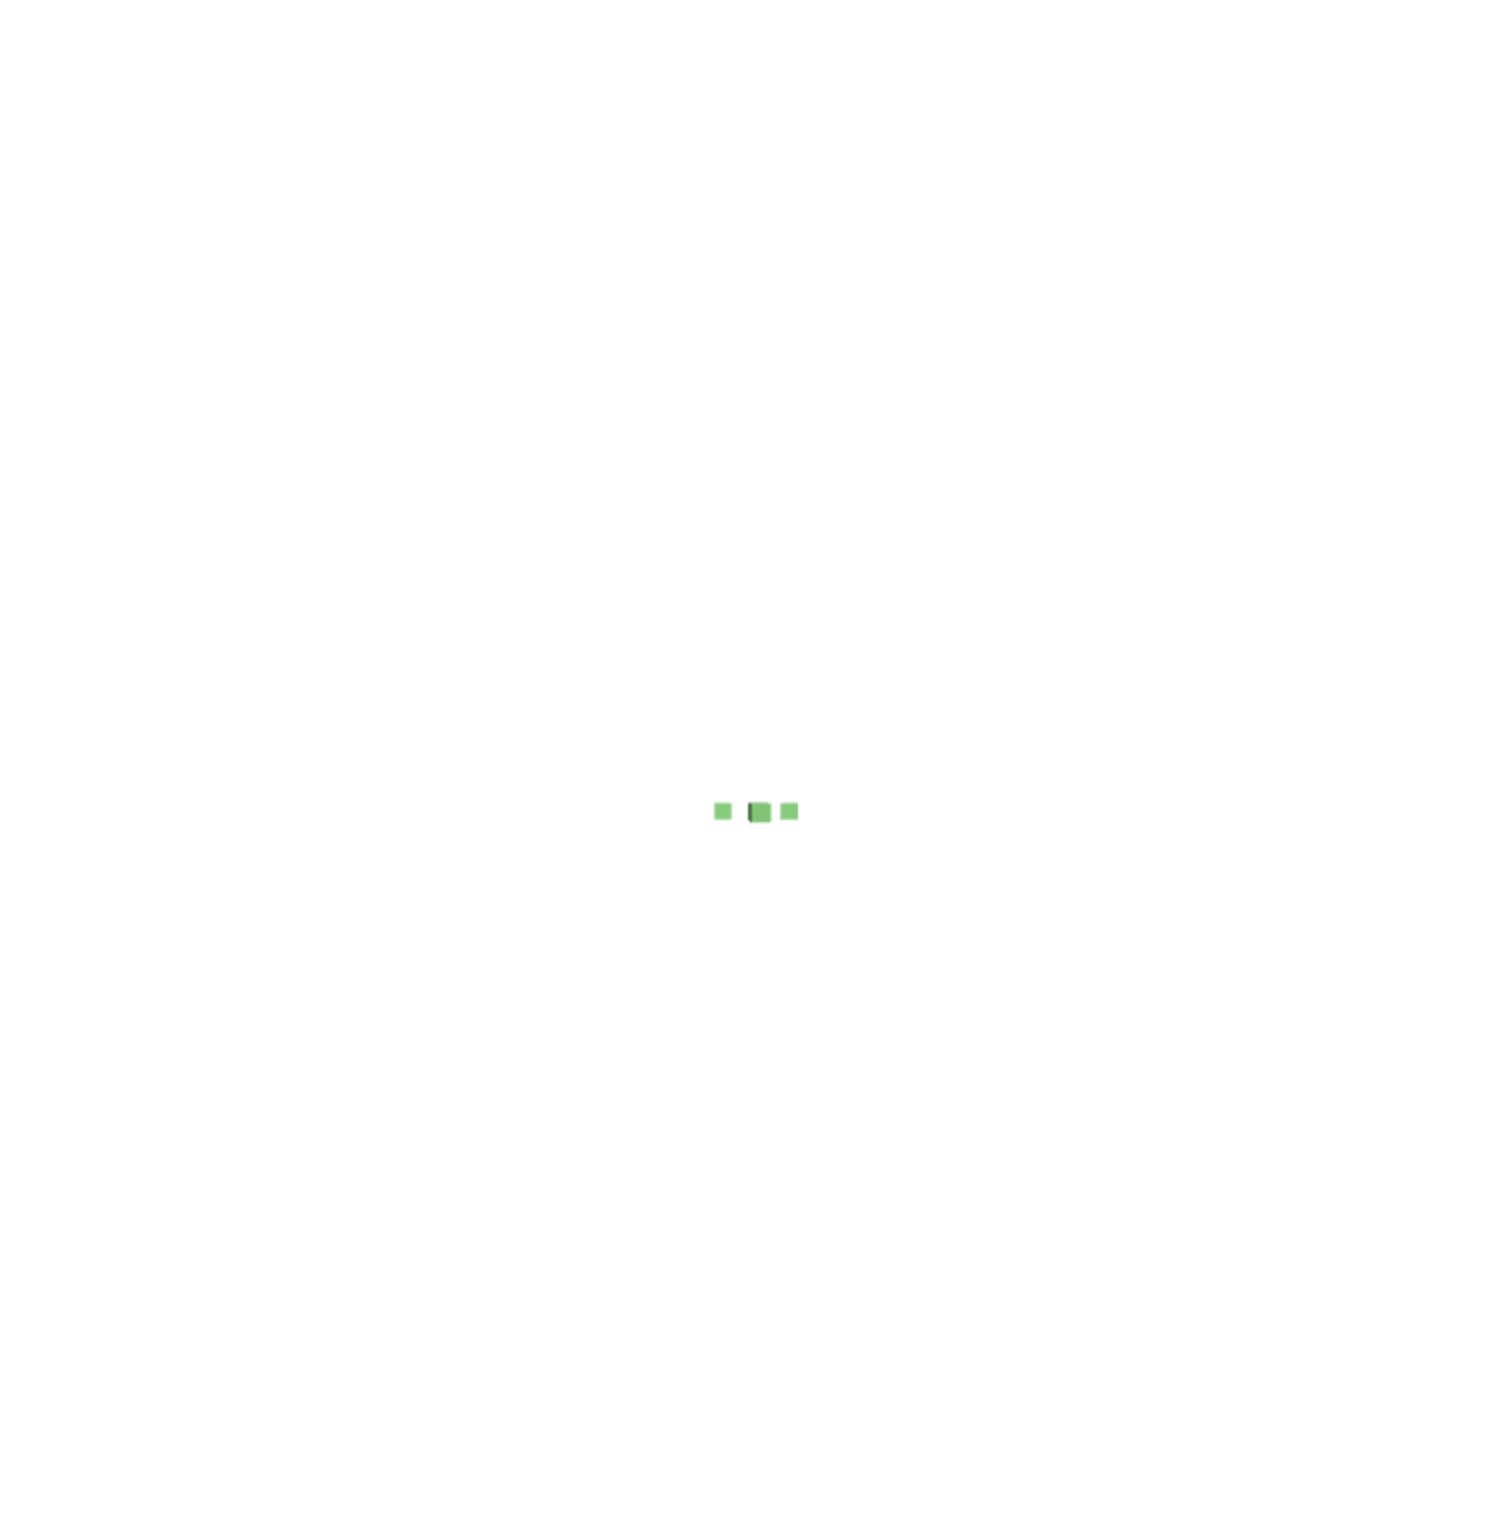
\includegraphics[width=\linewidth]{JetUML_V0S1.png}
        \caption{First commit seen from a top angle } 
        \label{fig:JetUML_V0S1_0}
    \end{subfigure}
    \hspace*{\fill}
    \begin{subfigure}{0.42\textwidth}
        
\includegraphics[width=\linewidth]{JetUML_V0S1_1.png}
        \caption{First commit seen from a mid angle} 
        \label{fig:JetUML_V0S1_1}
    \end{subfigure}
    \caption{First commit of JetUML made on Wed, 07 Jan 2015, 18:59. Three entities have been added; they are depicted with the green color. The entity in the middle represents the license file, taller because its size is bigger than other files.} 
    \label{fig:JetUML_V0S1}
\end{figure}

Here we present some results that we found looking at the graphical evolution of JetUML. 
To keep this section short, we report only a subset of the most active commits. 
\bigbreak
The repository's history starts on January 7, 2015, when Martin Robillard made the first commit. 
This commit added three files: README, a license, and a gitingore. 
Figure \ref{fig:JetUML_V0S1} represents it with three entities. They all have the same shape because we did not adopt different shapes in the specification, but the height is different. The license file is taller than other entities because of its bigger size. 
\bigbreak
Fifteen minutes later, he pushed the initial codebase of a project named Violet, composed of 83 files and an updated version of the gitignore file. This commit is represented in figure \ref{fig:JetUML_V0S2}, where 83 green entities represent added files, one yellow entity represents the updated gitignore files, and two gray entities, the README and the license files added before, that were not touched.
\bigbreak
Forty minutes later, he made the first big refactor of the system, whose goal was to move the position of some fields in each class. This refactoring involved 49 files, and as we can see from figure \ref{fig:JetUML_V0S3} they are marked in yellow. 
\bigbreak
Three days later, after a series of delicate development tasks had been continuously made, he moved some classes from the Violet folder to a new one named Violetta. As we can notice from figure \ref{fig:JetUML_V0S4} moved classes are represented with light blue. 
\bigbreak
Twenty-six commits later, on January 22, 2015, they moved classes from Violet and Violetta under the JetUML package. This commit, represented in figure \ref{fig:JetUML_V0S5}, was the first when JetUML was officially used; it denotes its birth. 
\bigbreak
After this first implementation, the system gradually grew, doubling its size in less than two years. 
During this time interval, they have been made only small commits to solve open issues. However, some exceptions were displayed in figure \ref{fig:JetUML_V0S6} and \ref{fig:JetUML_V0S7} where many files were modified because they had to update classes copyright lines. 
\bigbreak
In November 2017, they removed "stg" from the path of all the Java classes part of the system. This commit is depicted in figure \ref{fig:JetUML_V0S8}, where we can observe 162 light blue entities. They represent classes moved from the "../ca/mcgill/cs/stg/jetuml/..." path to the 
"../ca/mcgill/cs/jetuml/..." path. Moreover, this commit also had 15 modified fields, and one added. 
\bigbreak
One last huge refactor was done in July 2020, two years later, again to change the copyright on every class. It is represented in figure \ref{fig:JetUML_V0S9}. In this figure, we can notice that there are many blank spots in the middle. This means that entities added in the early stages of the project have been removed and are no longer part of the system. At that time, the system had 316 entities, and 241 were affected by this commit. 
\bigbreak
The last version of the system, created on Thu, May 12, 2022, counts 456 entities. 
\bigbreak
\textbf{Conclusion}
We manually inspected 2153 frames depicting the evolution of JetUML.
Thanks to the autoplay feature of SYN-Debugger, it was not an agonizing activity. \\
Occasionally JetUML needed to make huge commits involving most files on their repository. Nonetheless, they were spotted easily, thanks to the adopted visualization settings. 
Most of the commits involved few entities; this means that features were implemented gradually, maybe following an incremental or spiral development approach. 
With this grouping strategy, it was hard to understand the regularity and the speed of the development process. This is normal when we traverse the history by commit rather than traverse it by time. 

\begin{figure}[ht]
    \begin{subfigure}{0.32\textwidth}
        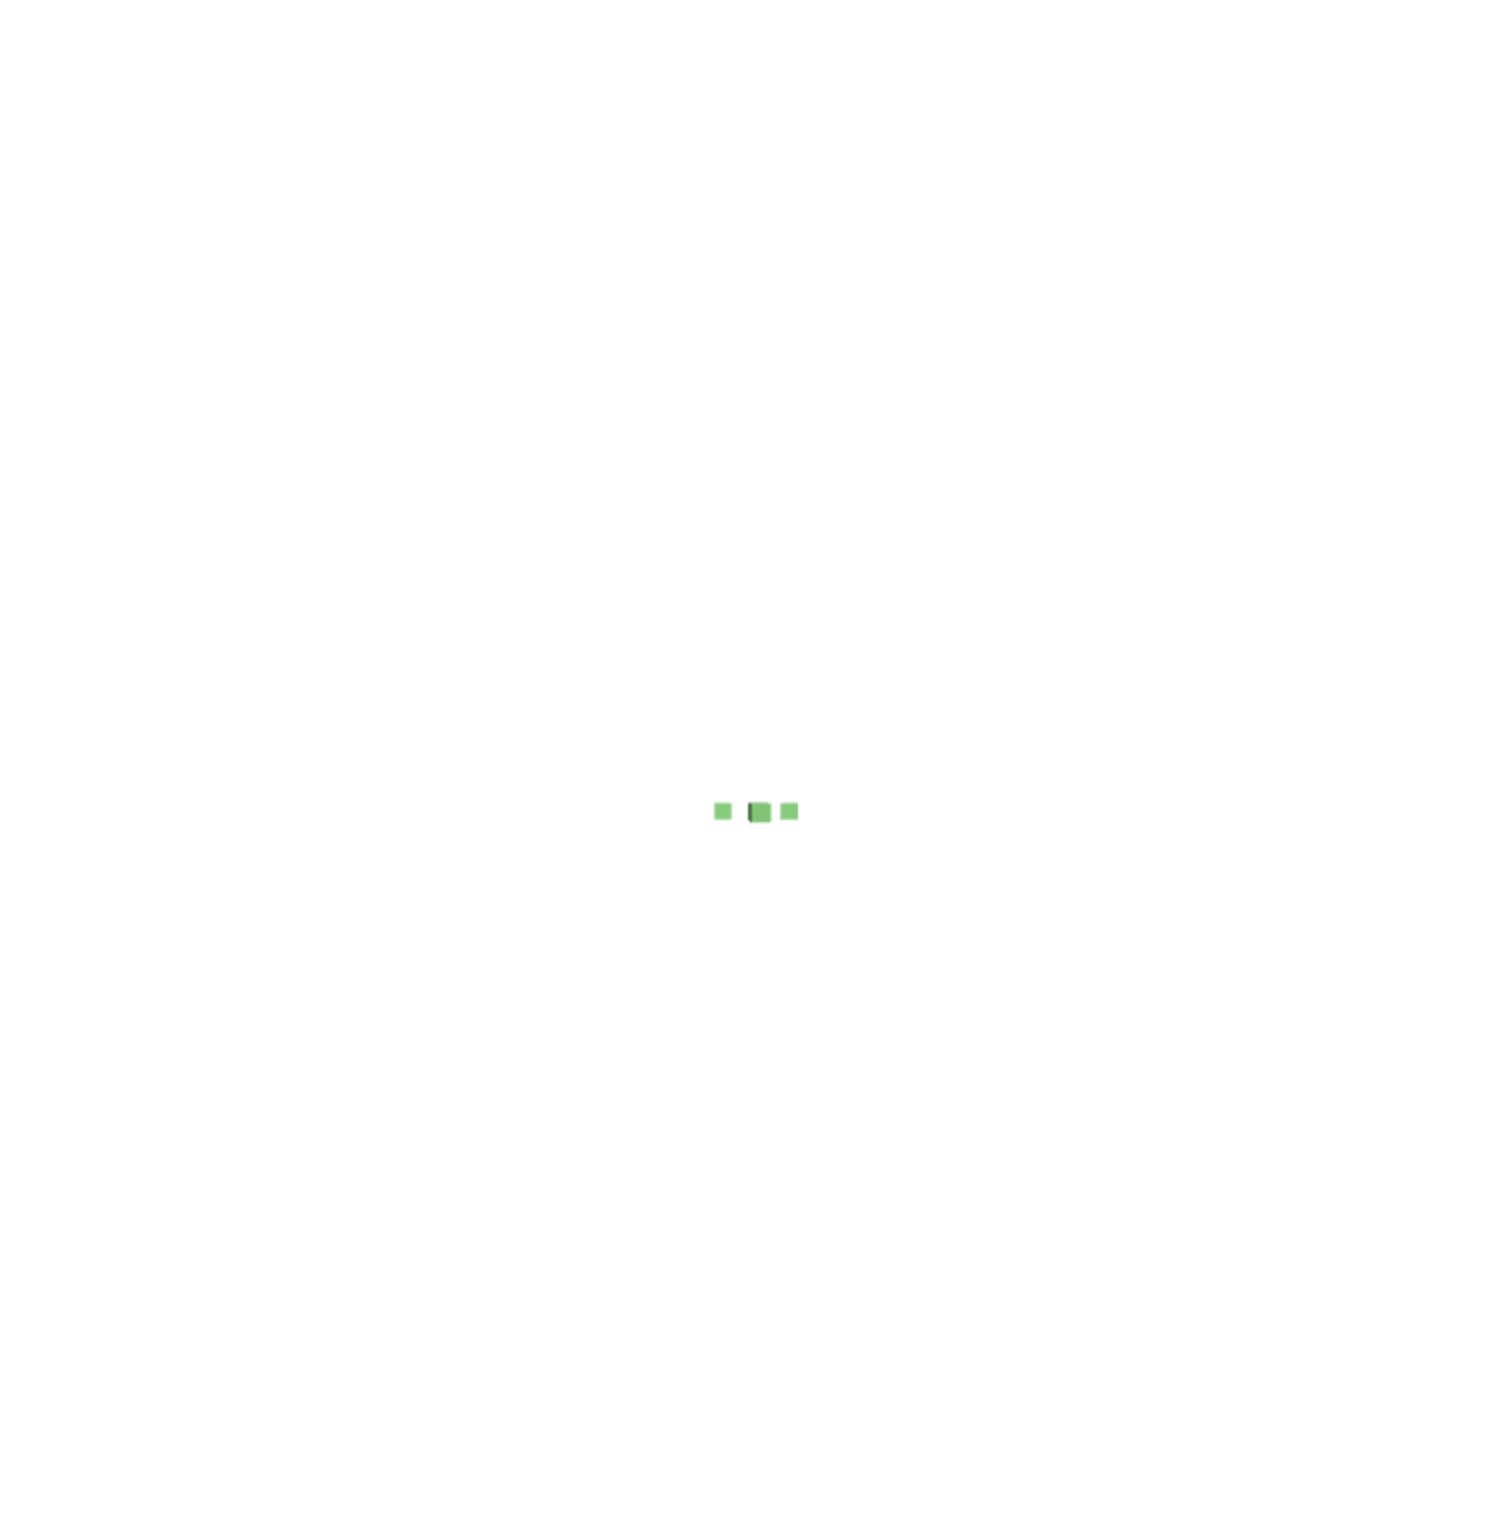
\includegraphics[width=\linewidth]{JetUML_V0S1.png}
        \caption{07 Jan 2015, 18:59 \linebreak Initial commit} 
        \label{fig:JetUML_V0S1_3}
    \end{subfigure}
    \hspace*{\fill}
    \begin{subfigure}{0.32\textwidth}
        
\includegraphics[width=\linewidth]{JetUML_V0S2.png}
        \caption{07 Jan 2015, 19:14 \linebreak  Initial Revision} 
        \label{fig:JetUML_V0S2}
    \end{subfigure}
    \hspace*{\fill}
    \begin{subfigure}{0.32\textwidth}
        
\includegraphics[width=\linewidth]{JetUML_V0S3.png}
        \caption{07 Jan 2015, 19:57 \linebreak  \#1 Move all fields} 
        \label{fig:JetUML_V0S3}
    \end{subfigure}
    \hspace*{\fill}
    \medskip
    \begin{subfigure}{0.32\textwidth}
        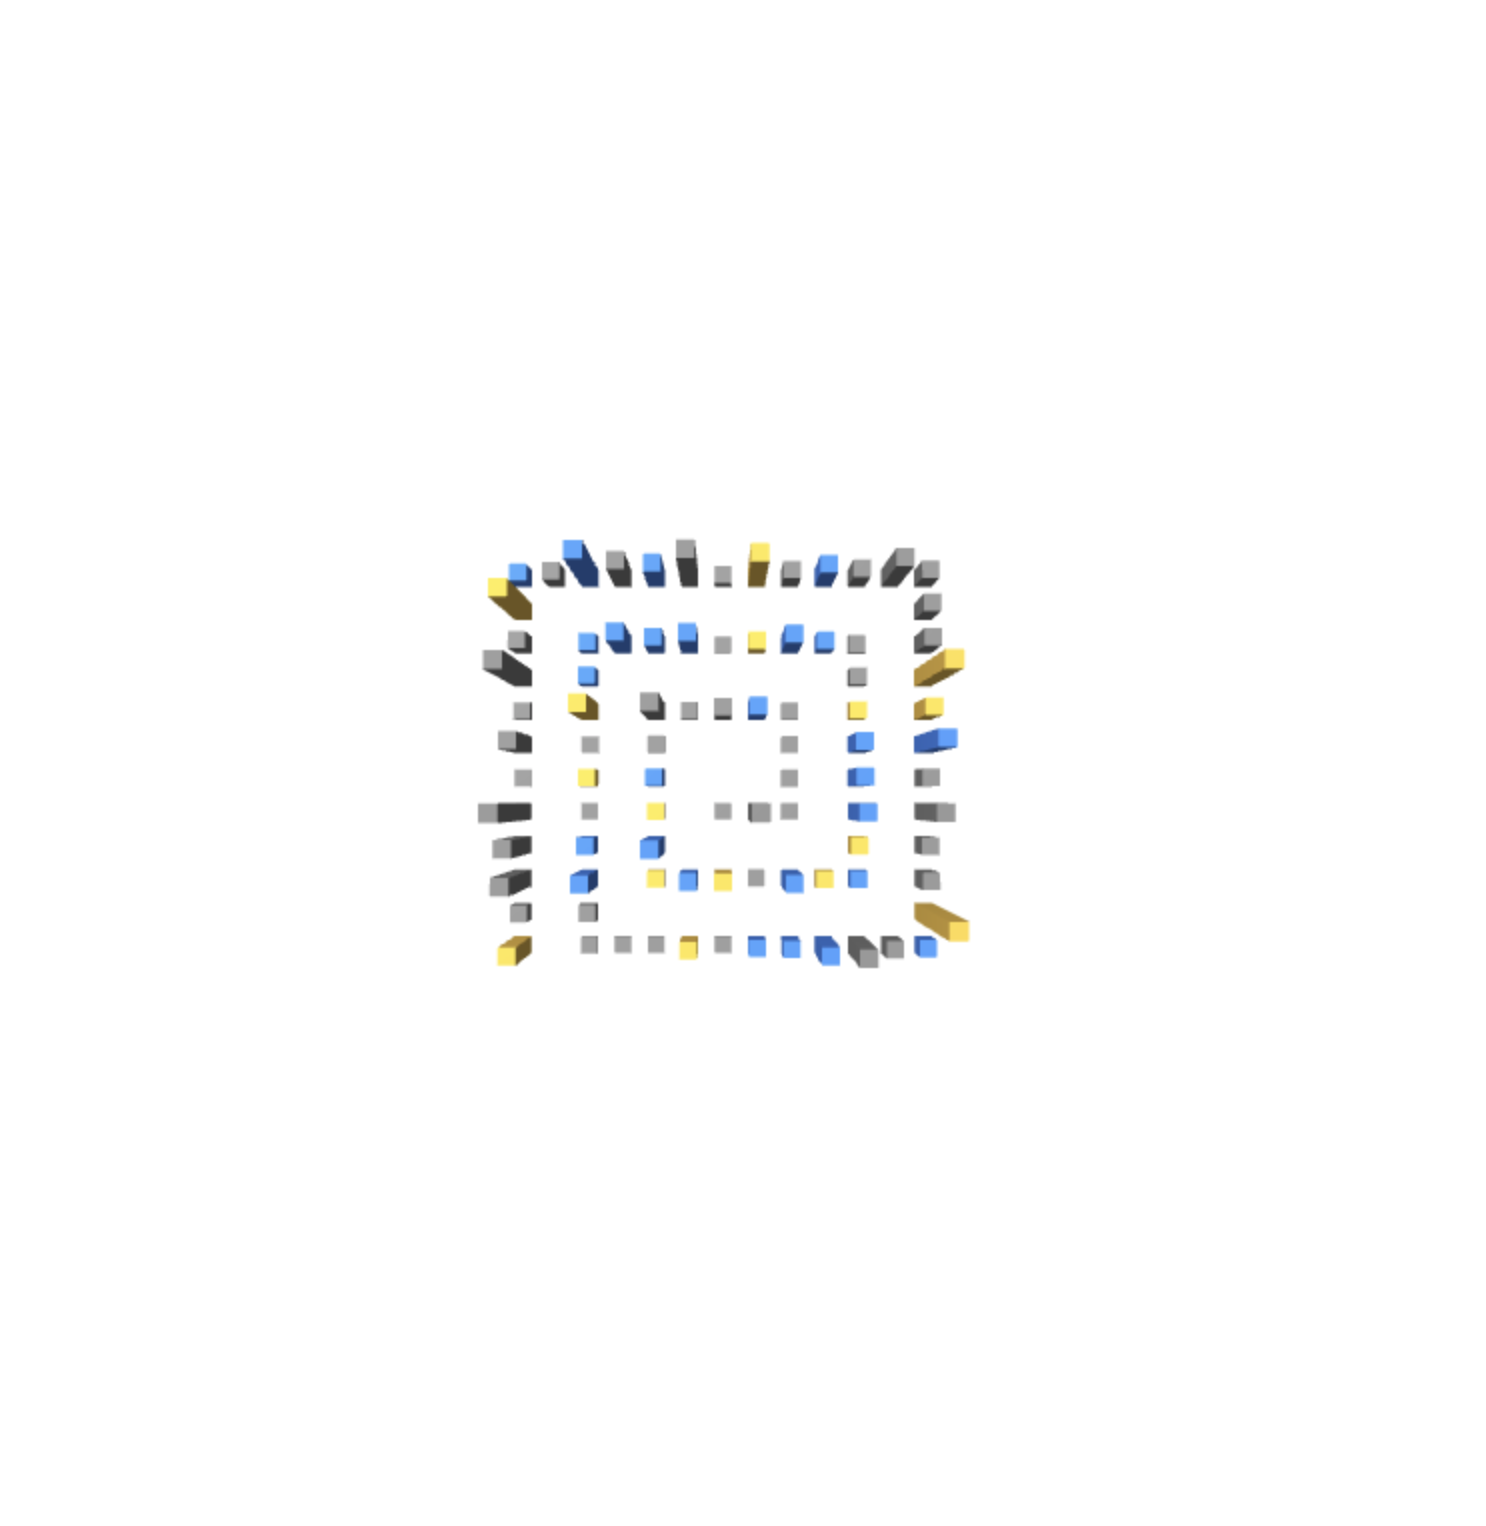
\includegraphics[width=\linewidth]{JetUML_V0S4.png}
        \caption{10 Jan 2015 \linebreak  \#8 Moved to a dedicated ...} 
        \label{fig:JetUML_V0S4}
    \end{subfigure}
    \hspace*{\fill}
    \begin{subfigure}{0.32\textwidth}
        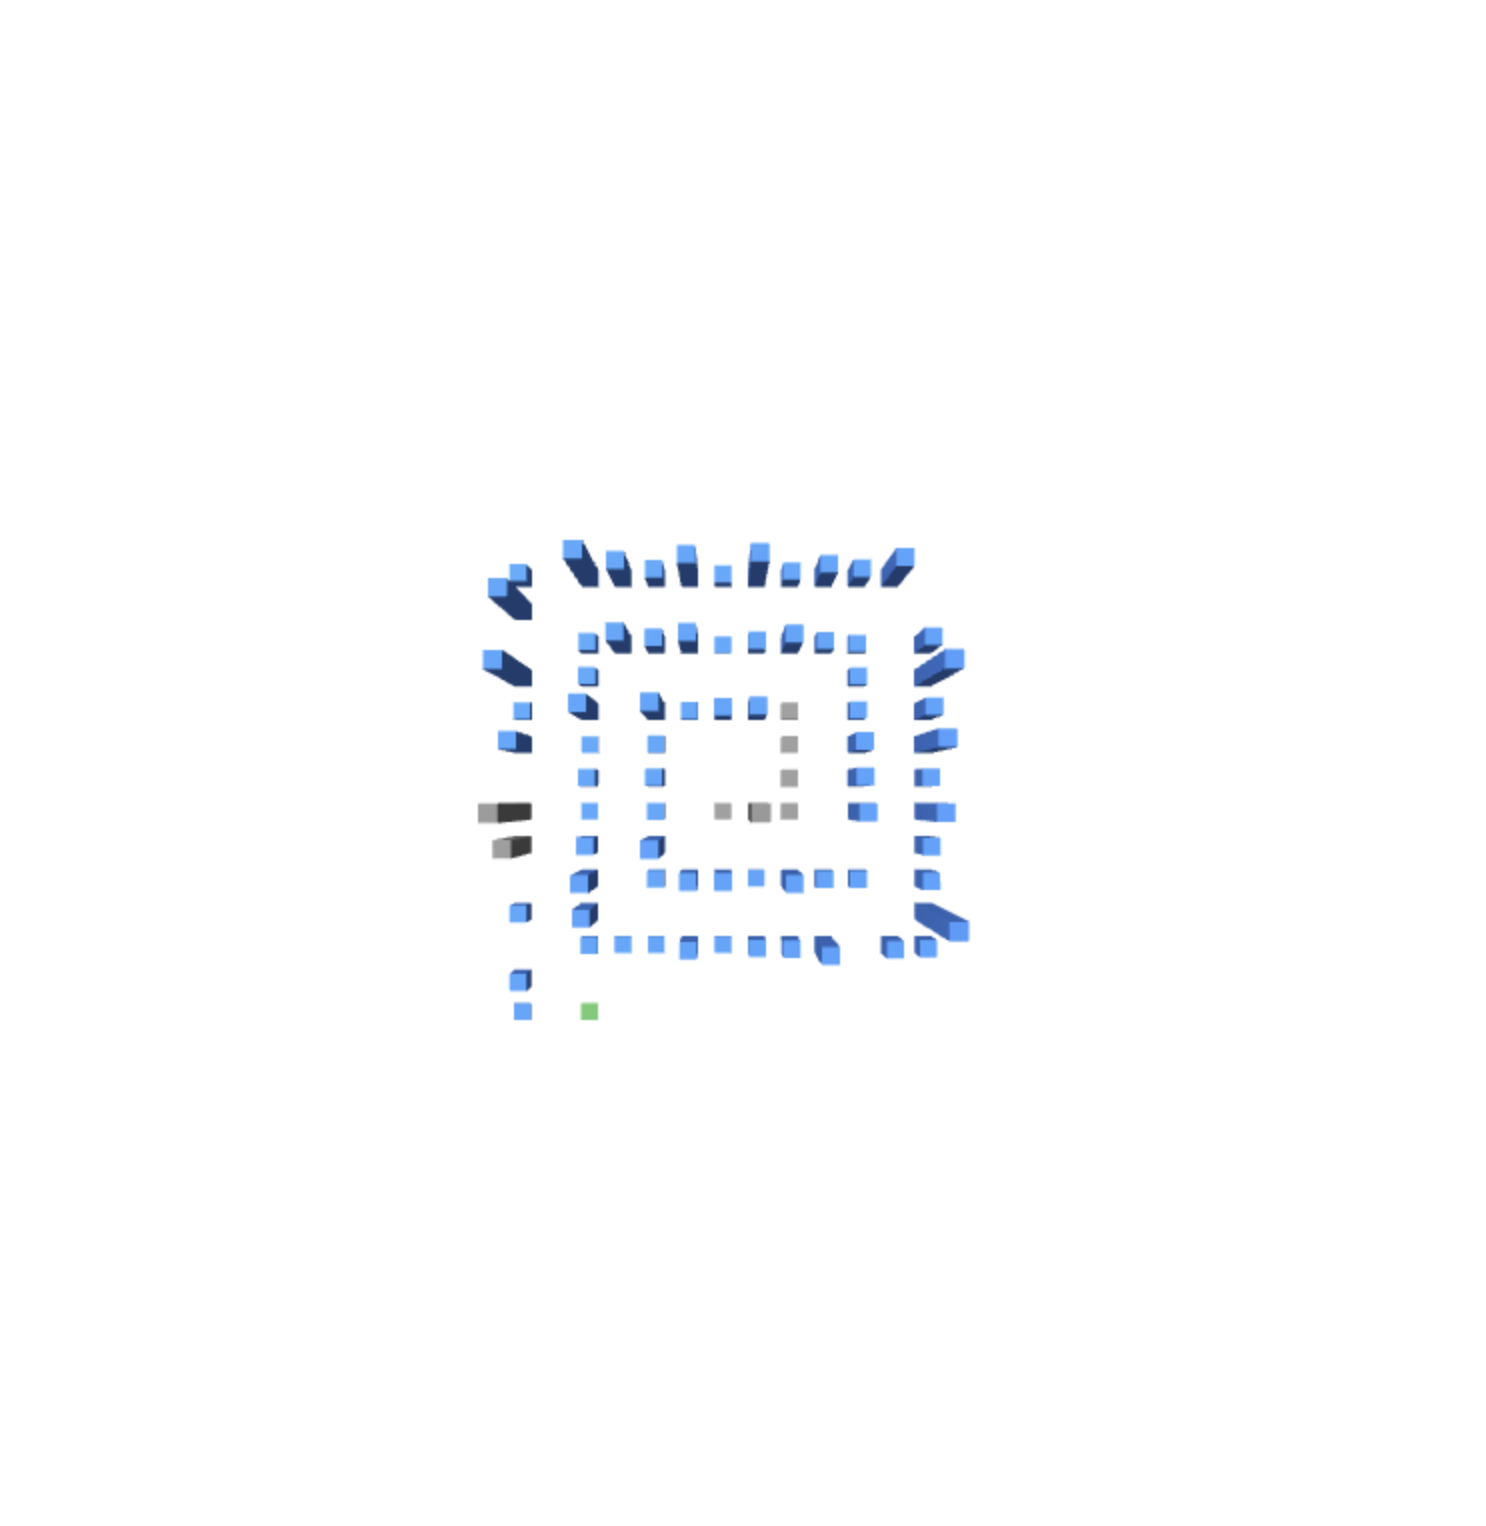
\includegraphics[width=\linewidth]{JetUML_V0S5.png}
        \caption{22 Jan 2015 \linebreak  \#27 Renamed the packages} 
        \label{fig:JetUML_V0S5}
    \end{subfigure}
    \hspace*{\fill}
    \begin{subfigure}{0.32\textwidth}
        
\includegraphics[width=\linewidth]{JetUML_V0S6.png}
        \caption{16 Oct 2015 \linebreak  \#3 New copyright block on ...} 
        \label{fig:JetUML_V0S6}
    \end{subfigure}
    \hspace*{\fill}
    \medskip
    \begin{subfigure}{0.32\textwidth}
        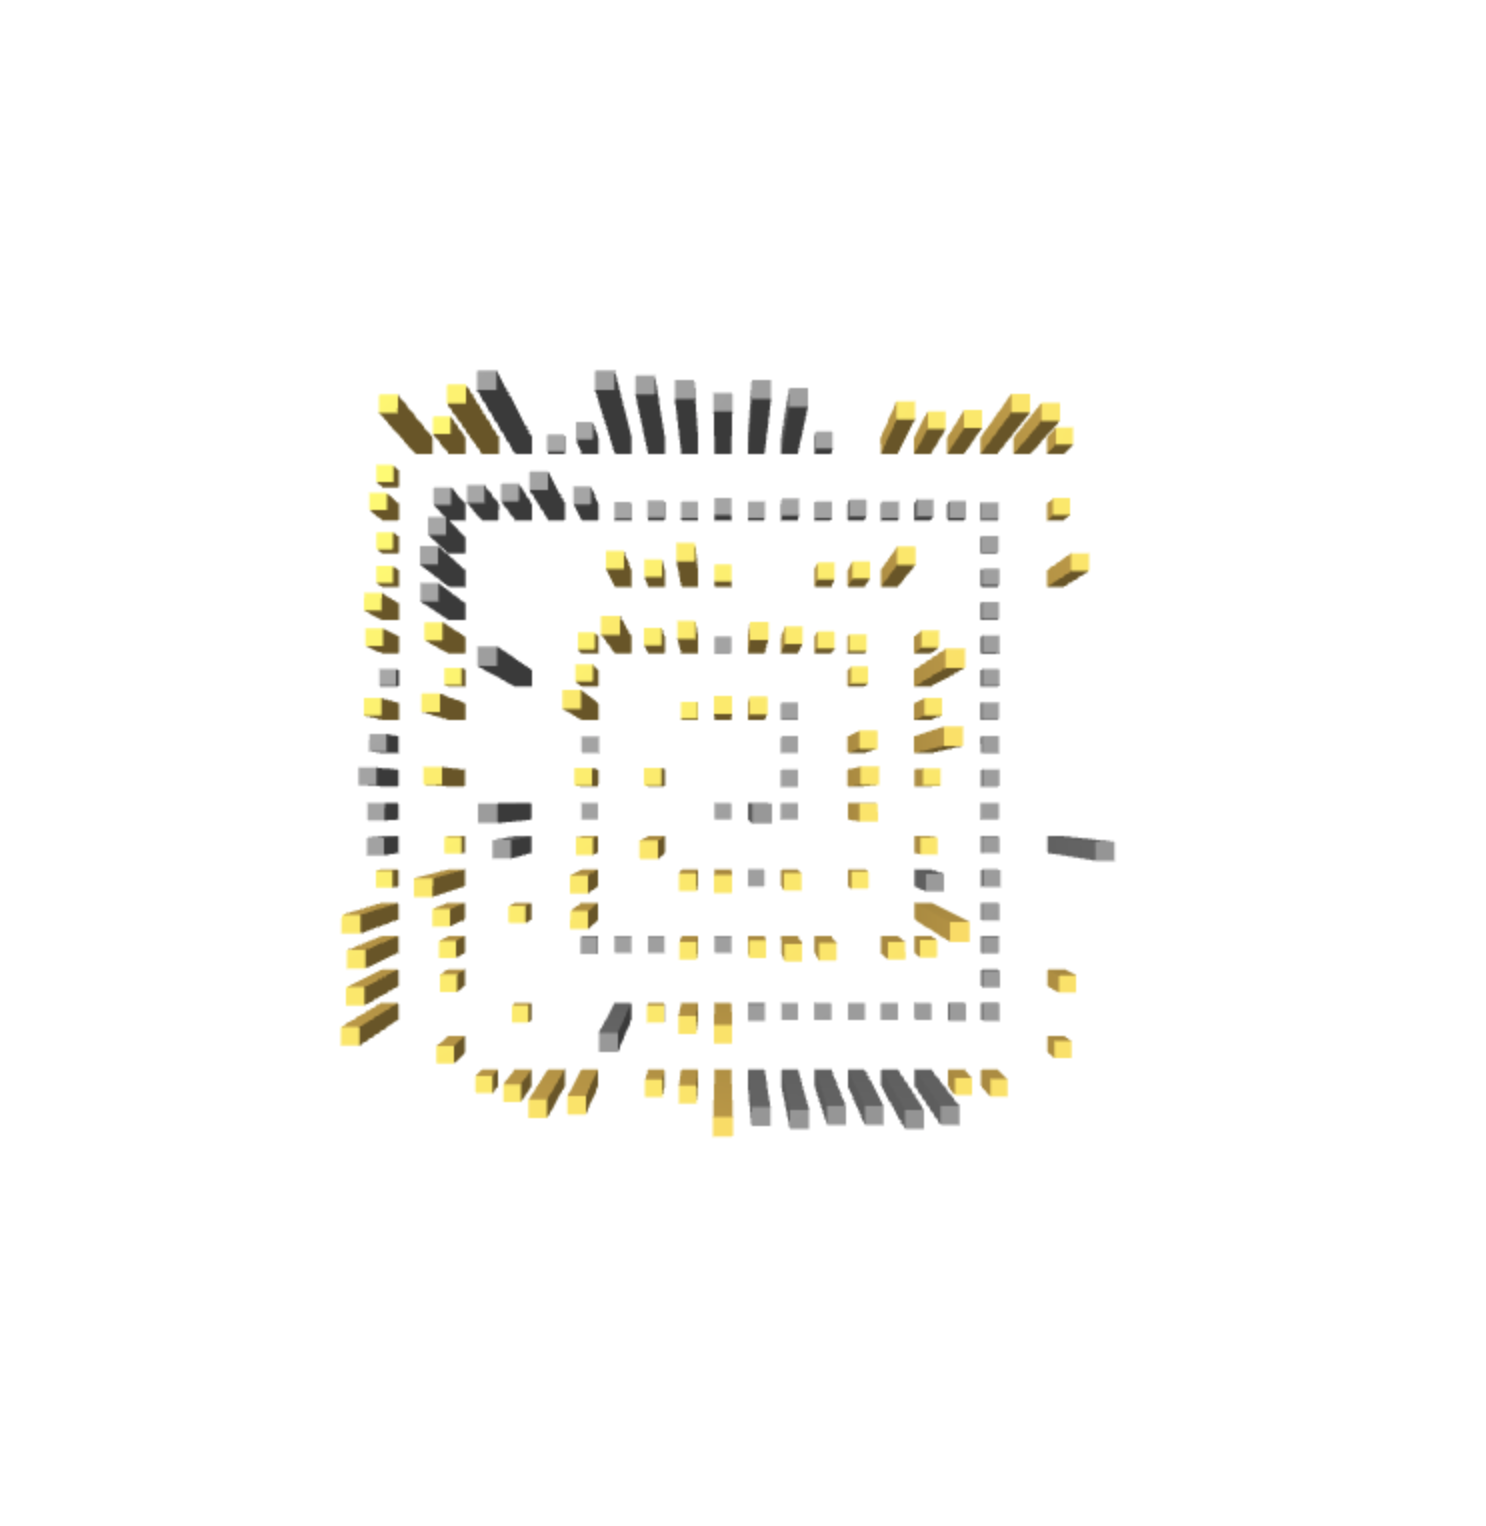
\includegraphics[width=\linewidth]{JetUML_V0S7.png}
        \caption{17 Jan 2016 \linebreak  \#146 Updated the copyright ...}
         \label{fig:JetUML_V0S7}
    \end{subfigure}
    \hspace*{\fill}
    \begin{subfigure}{0.32\textwidth}
        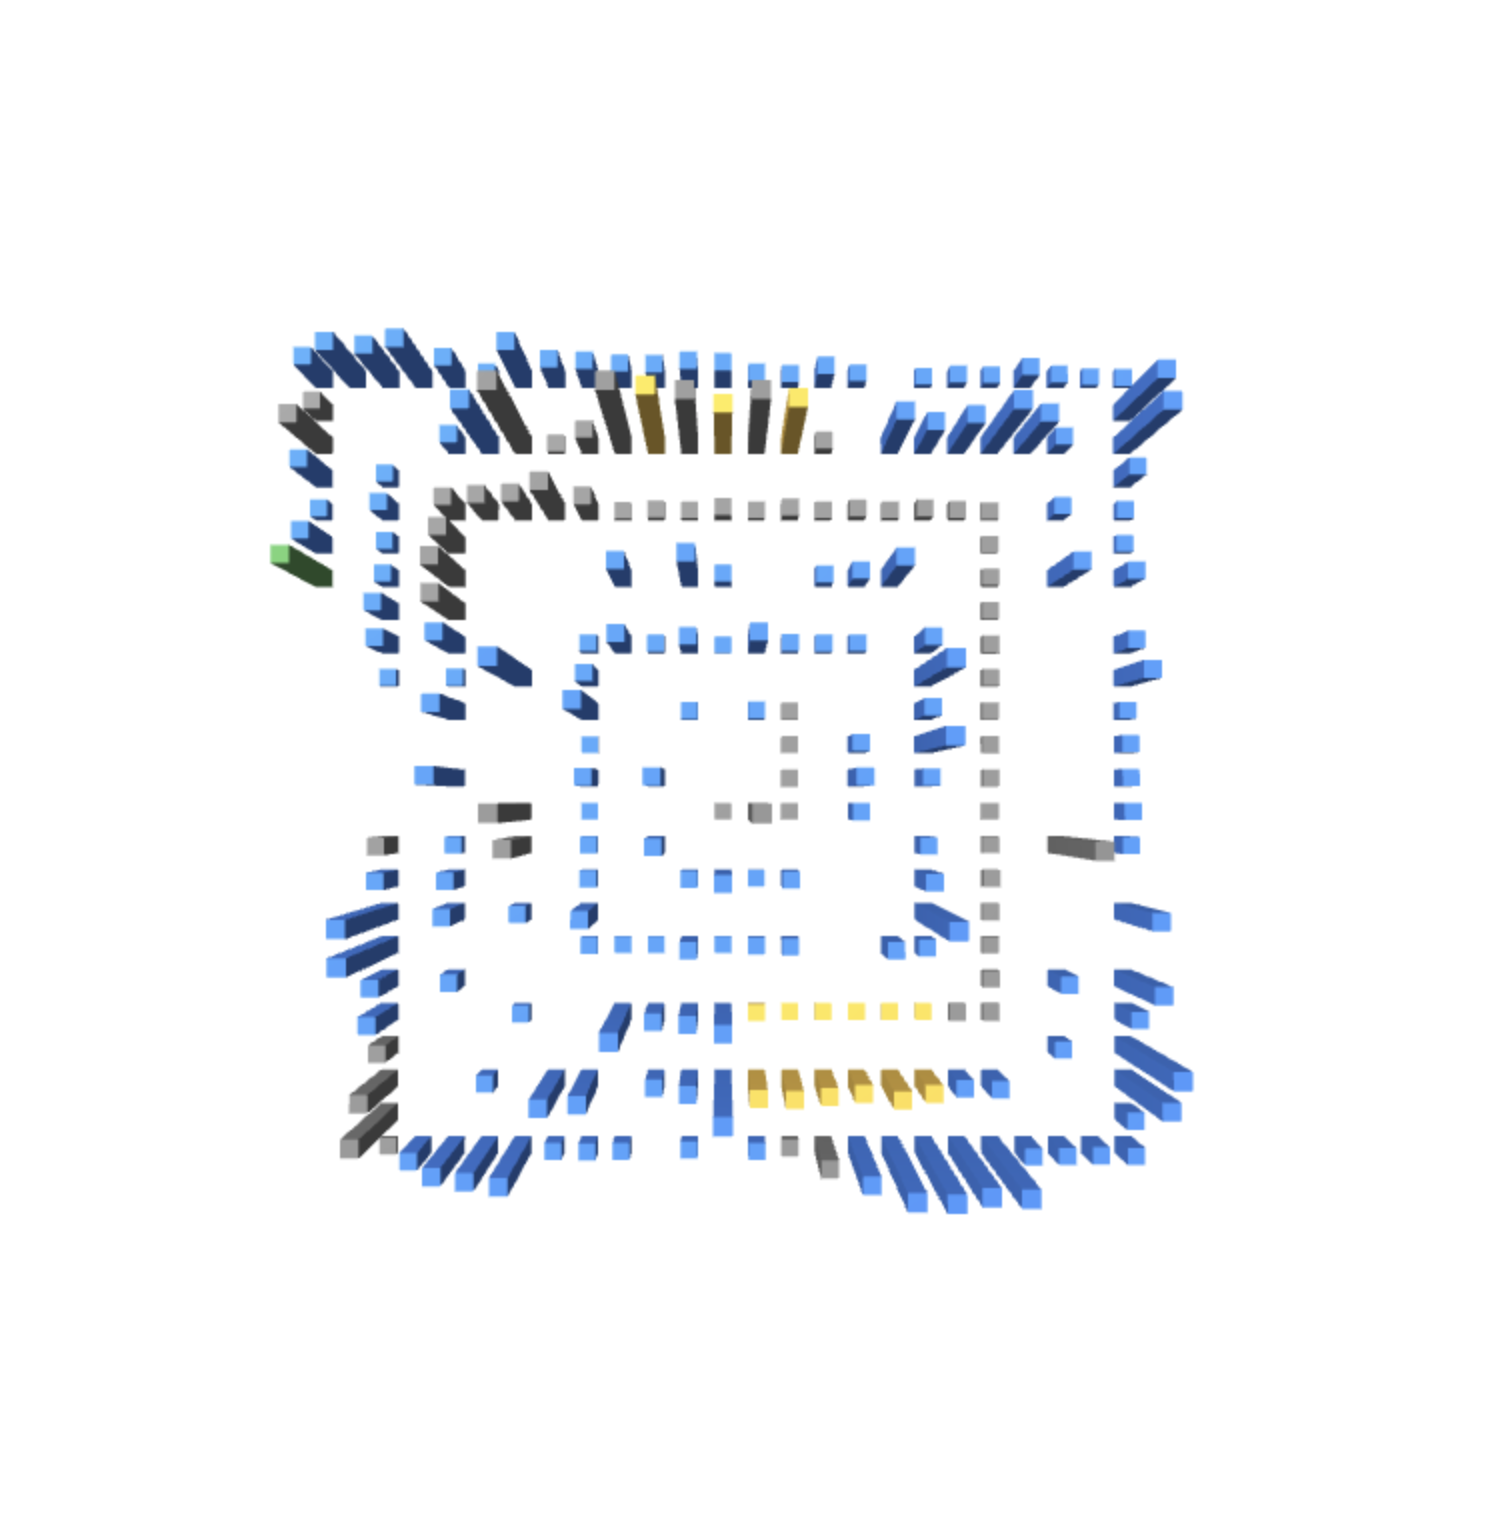
\includegraphics[width=\linewidth]{JetUML_V0S8.png}
        \caption{26 Nov 2017 \linebreak  \#212 Remove stg from name} 
        \label{fig:JetUML_V0S8}
    \end{subfigure}
    \hspace*{\fill}
    \begin{subfigure}{0.32\textwidth}
        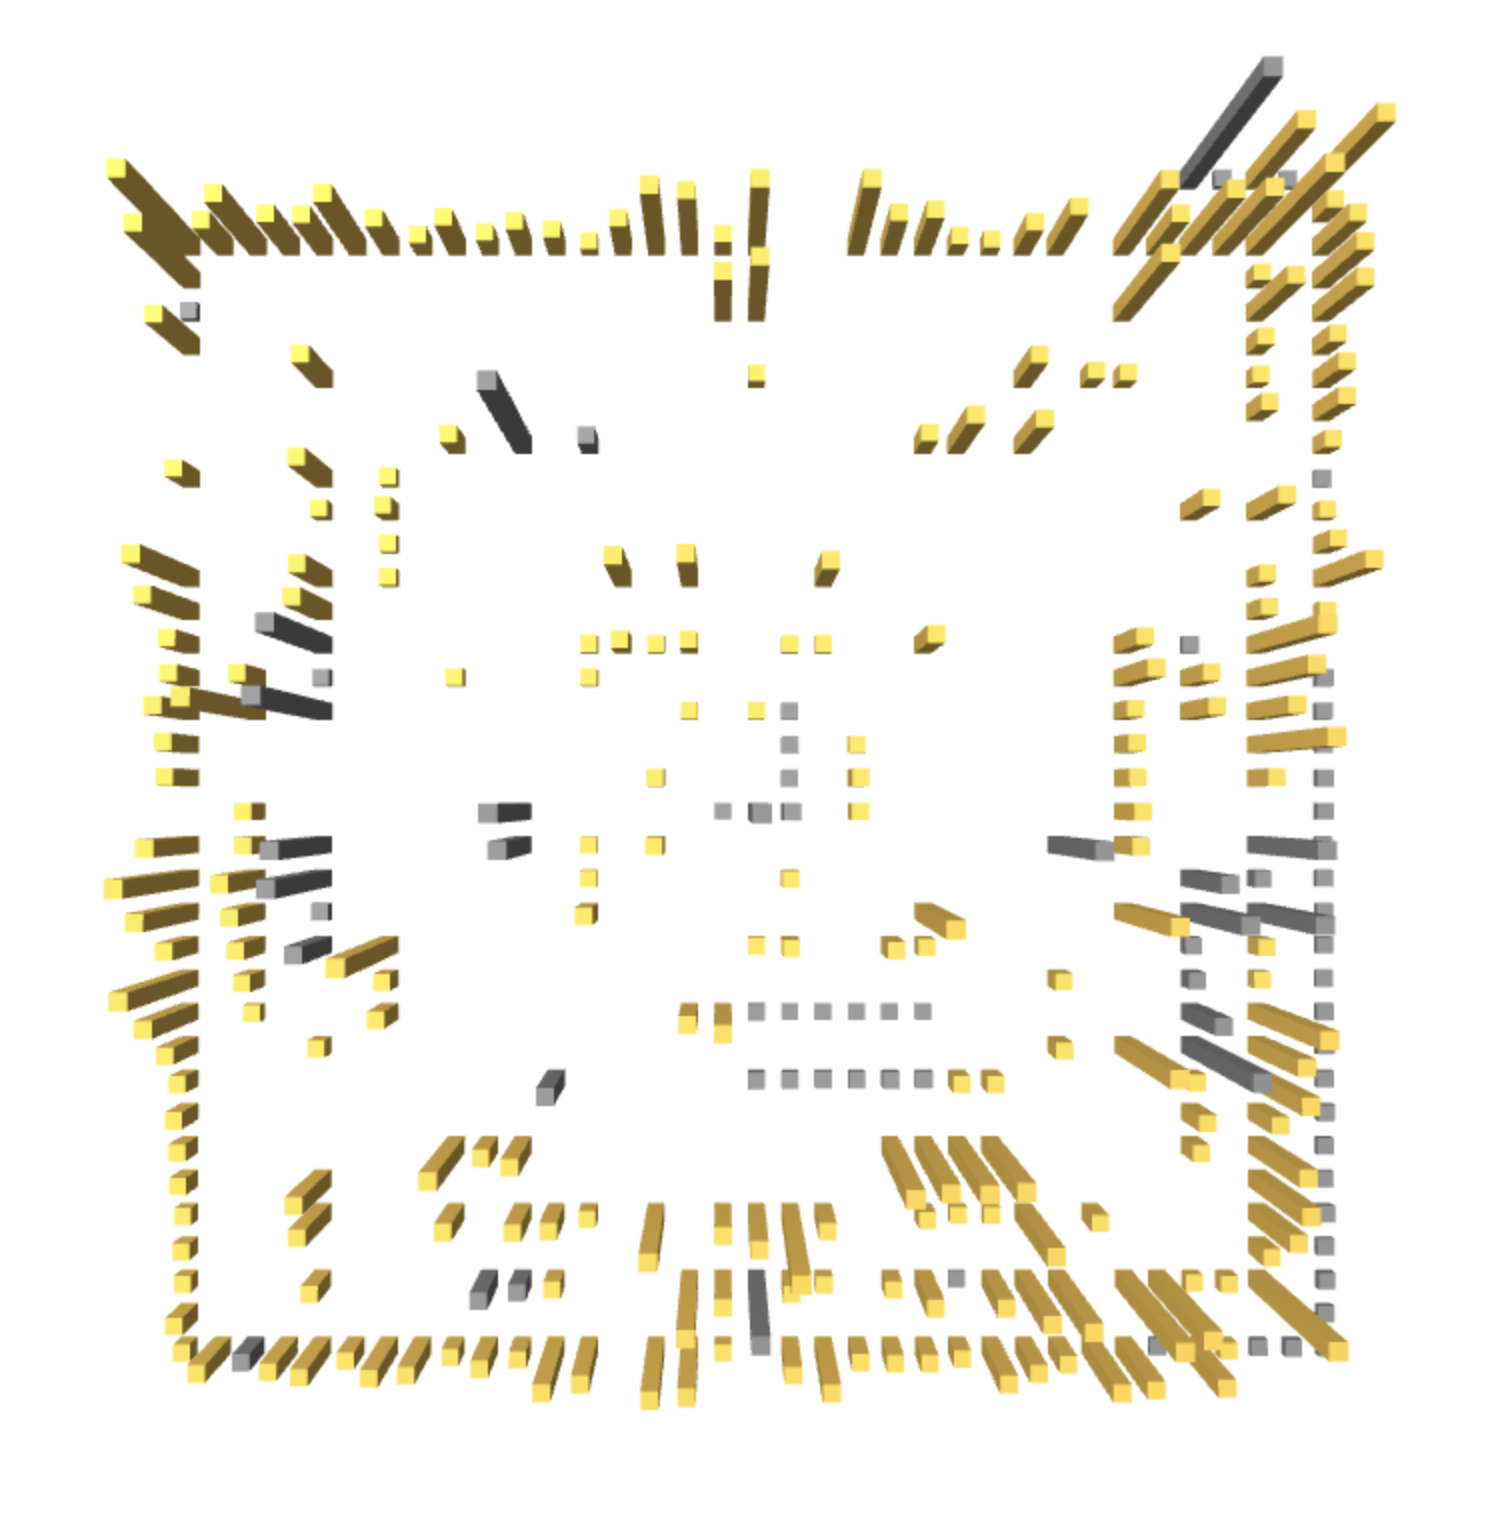
\includegraphics[width=\linewidth]{JetUML_V0S9.png}
        \caption{22 Jul 2020 \linebreak  \#374 Fix copyrights} 
        \label{fig:JetUML_V0S9}
    \end{subfigure}
    \hspace*{\fill}
    \medskip
    \caption{
        Subset of the biggest commits in JetUML. Figure \ref{fig:JetUML_V0S1_3} represent the first commit. In Figure \ref{fig:JetUML_V0S2} they pushed the code of Violetta. Figure \ref{fig:JetUML_V0S3} depicts their first refactoring. In Figure \ref{fig:JetUML_V0S4} they moved some classes from Violet to Violetta. In Figure  \ref{fig:JetUML_V0S5} they moved most of them under JetUML. In Figure \ref{fig:JetUML_V0S6}, \ref{fig:JetUML_V0S7} and \ref{fig:JetUML_V0S9} are depicted three refactoring activities to fix copyrights. In Figure \ref{fig:JetUML_V0S8} most of the entities are painted with blue because they changed their path.} 
    \label{fig:JetUML_V0}
\end{figure}

\clearpage
\section{JetUML 2}
\textbf{Goal of this visualization}
With this visualization, we want to see how the repository evolved through its first six months. 
The authors of JetUML, during this interval of time, made seven pre-releases of the system. 
Moreover, we want to show what an aging strategy of one month with ten steps looks like. 

\bigbreak
View specification adopted: 
\begin{itemize}
    \item \texttt{versionGroupingStrategy}: timestamp.
    \item \texttt{versionGroupingChunkSize}: 2'629'743 (1 month). 
    \item \texttt{colorPalette}: default.
    \item \texttt{agingGroupingStrategy}: timestamp.
    \item \texttt{agingStepSize}: 2'629'743 (1 month).
    \item \texttt{agingSteps}: 10 steps.
    \item \texttt{mapperMetricName}: SIZE. 
    \item \texttt{fileTypeShape}: all BOX. 
    \item \texttt{fileTypeOpacity}: all 1. 
\end{itemize}

\textbf{Results}
\autoref{fig:JetUML_V1} shows the evolution of JetUML during its first 6 months. \autoref{fig:JetUML_V1S1} shows the state of the repository after its first month. All the entities are painted with the color representing the last action made on that file. All the colors are bright because the age of all the files is set to 0 since the time elapsed between their last action and the last commit of the visualization cannot be higher than one month. The second month is depicted in \autoref{fig:JetUML_V1S2}. Here we can easily spot older entities as they are darker than others. This means that some files had not been touched since the first month at the end of the second month. In the third and the fourth month, more or less the same amount of files was updated. However, in the fifth month, only three entities were modified; consequently, all the others are darker because they are older. 
At the end of the sixth month, two entities were added and modified. However, most of the entities were still getting older. 

\textbf{Conclusion}
We have seen how different is the timestamp strategy compared to what we saw in the first visualization. Here, the number of frames does not depend upon the number of commits made; instead, it relies on the number of months part of the history. 
However, the choice of the aging strategy also played a crucial role in this visualization. It highlighted updated entities without hiding the last action made on the others. Looking at \autoref{fig:JetUML_V1S6}, we can immediately see that many files were added and never touched because their color looks dark green. The cause of this inactivity on the file may be related to the file type, which limits our visualization because we cannot infer the type in any way. 

% With this visualization, we want to see how all JetUML files evolved through time. 
% JetUML does not seem to have a fixed release cycle.
% Since its history spans eight years of activity; we initially chose a timestamp grouping strategy of one month. 
% As a consequence, we have 89 AnimationFrames. 
% In this first visualization, we do not care about the FileType of entities; we are interested in all of them. 
% Grouping commits monthly; we applied the same strategy to the aging to see how many months had passed since an entity was modified. 
% To summarize, the view specification of this visualization is the following:

% Figure \ref{fig:JetUML_V1} shows the first 6 month of evolution of JetUML. 
% We can infer many things by looking at these figures. In figure \ref{fig:JetUML_V1S1} 7 entities have been moved. 
% Most of them are files with the extension \texttt{.properties}, and perhaps they were involved in a refactoring activity since their path changed from
% \texttt{src/ca/mcgill/cs/stg/jetuml/...} to \texttt{src/ca/mcgill/cs/stg/jetuml/diagrams/...}. 
% At the end of their first month of activity, they had 135 files and made 127 commits. 
% We can see many files are still green. This means that they were added but never touched after. 
% An issue with this visualization is that we cannot distinguish Java files from others. 
% These added files are images. Therefore it is not a surprise that once added; they are never modified in the future. 
% In figure \ref{fig:JetUML_V1S2} where the second month is represented, we can see that some entities have a darker color. 
% This means that during the second month, they were not touched. 
% Comparing all the figures until figure \ref{fig:JetUML_V1S6} we can notice that many entities have the same behavior. 
% They were added and updated in the first month of activity (this is why they are yellow), and then they were never touched, becoming darker and darker each month. 

\begin{figure}[ht]
    \begin{subfigure}{0.48\textwidth}
    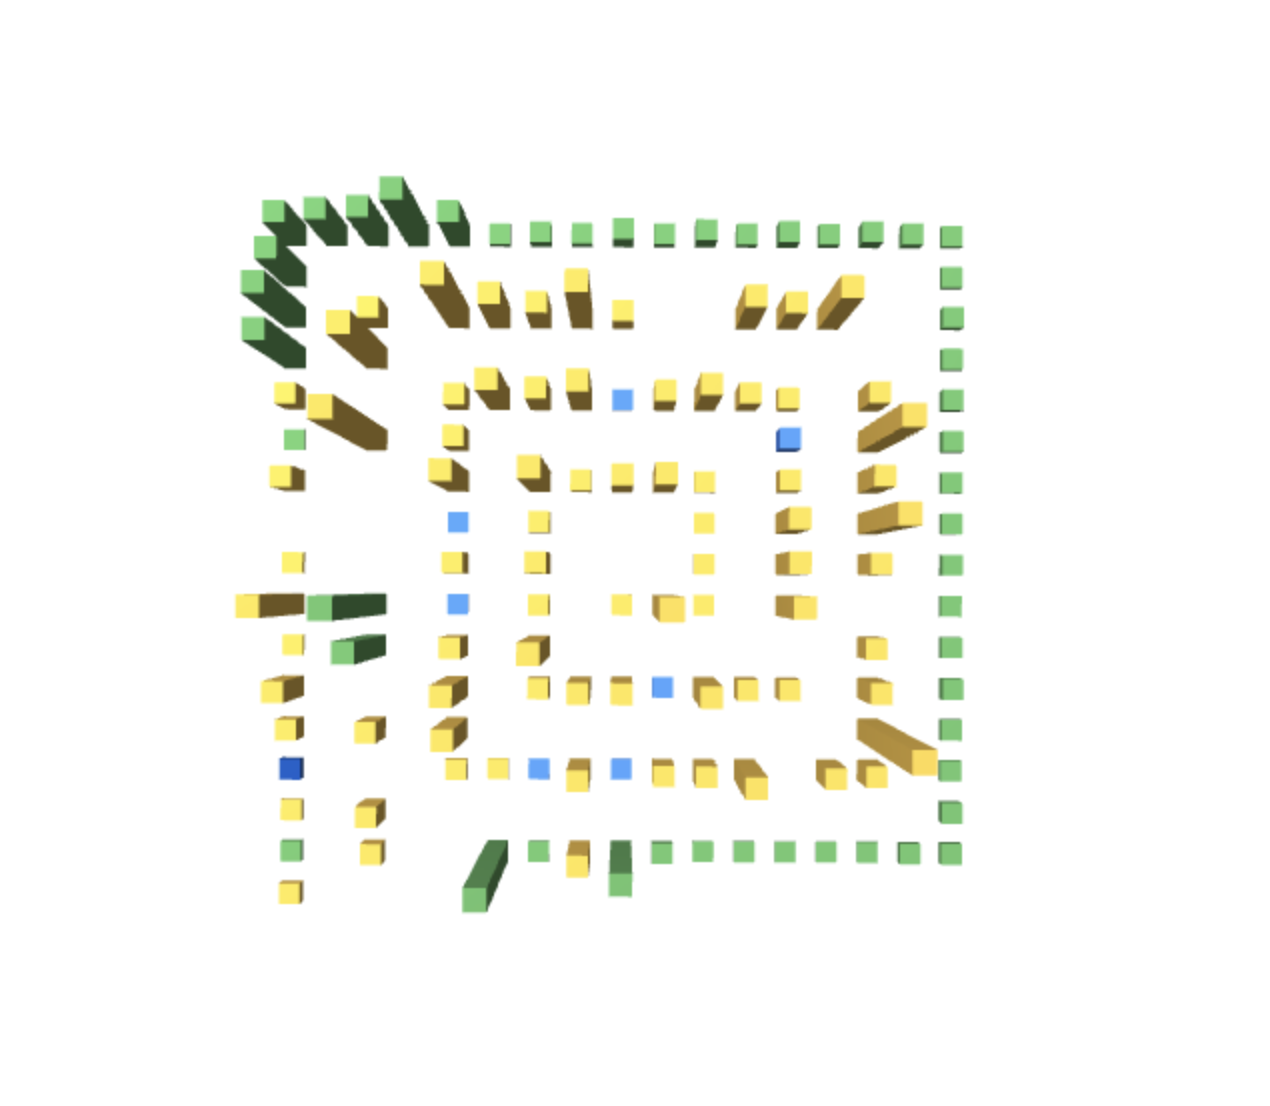
\includegraphics[width=\linewidth]{JetUML_V1S1.png}
    \caption{Month 1} \label{fig:JetUML_V1S1}
    \end{subfigure}\hspace*{\fill}
    \begin{subfigure}{0.48\textwidth}
        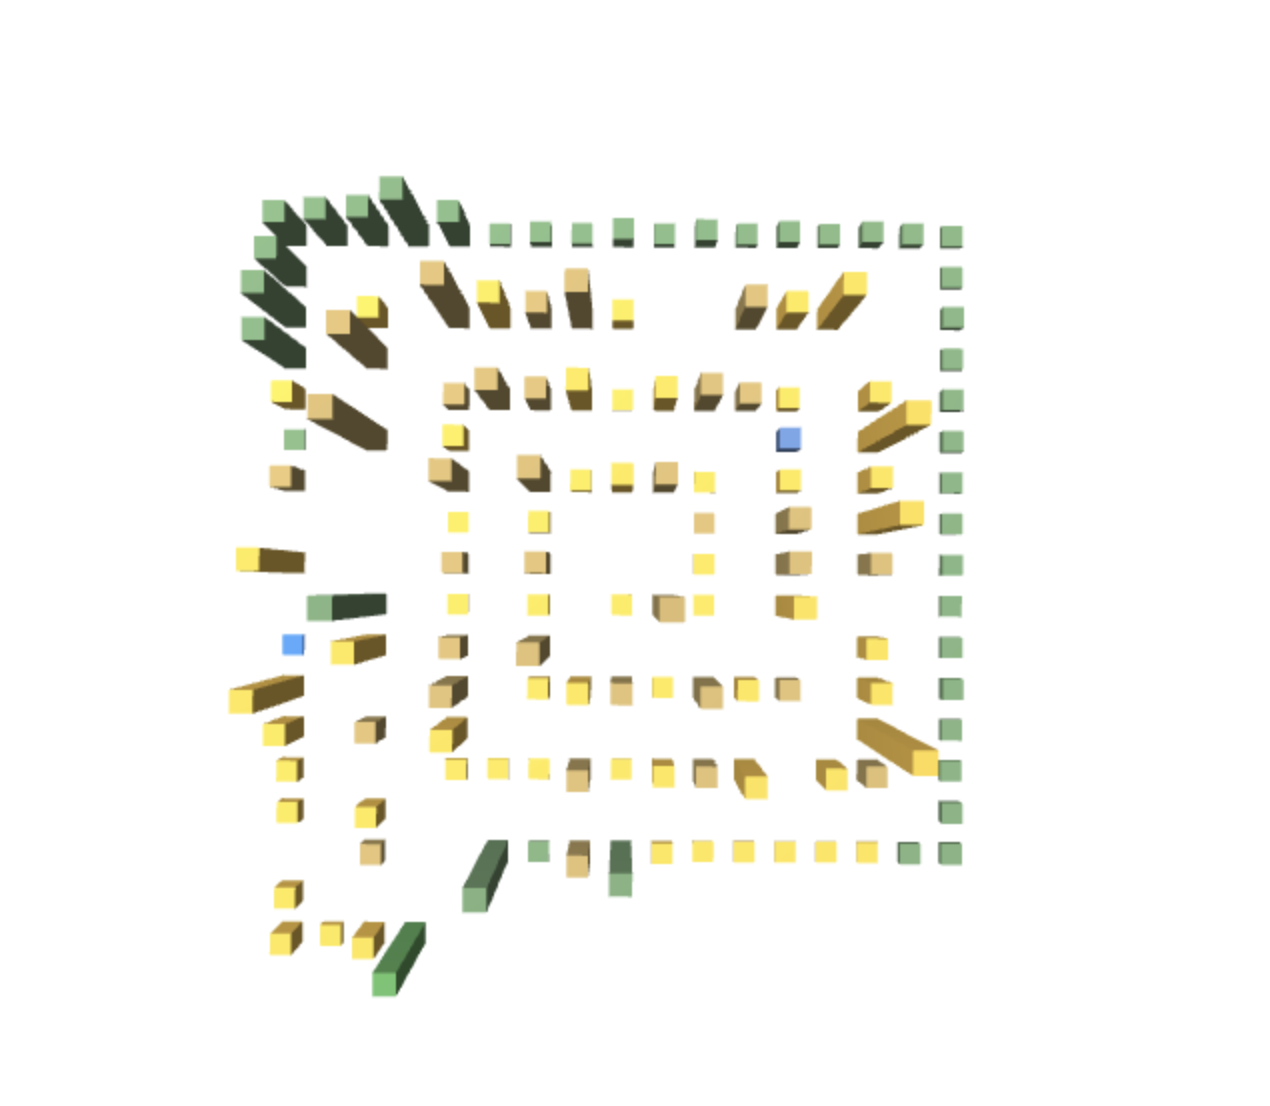
\includegraphics[width=\linewidth]{JetUML_V1S2.png}
        \caption{Month 2} \label{fig:JetUML_V1S2}
    \end{subfigure}
    
    \medskip
    \begin{subfigure}{0.48\textwidth}
        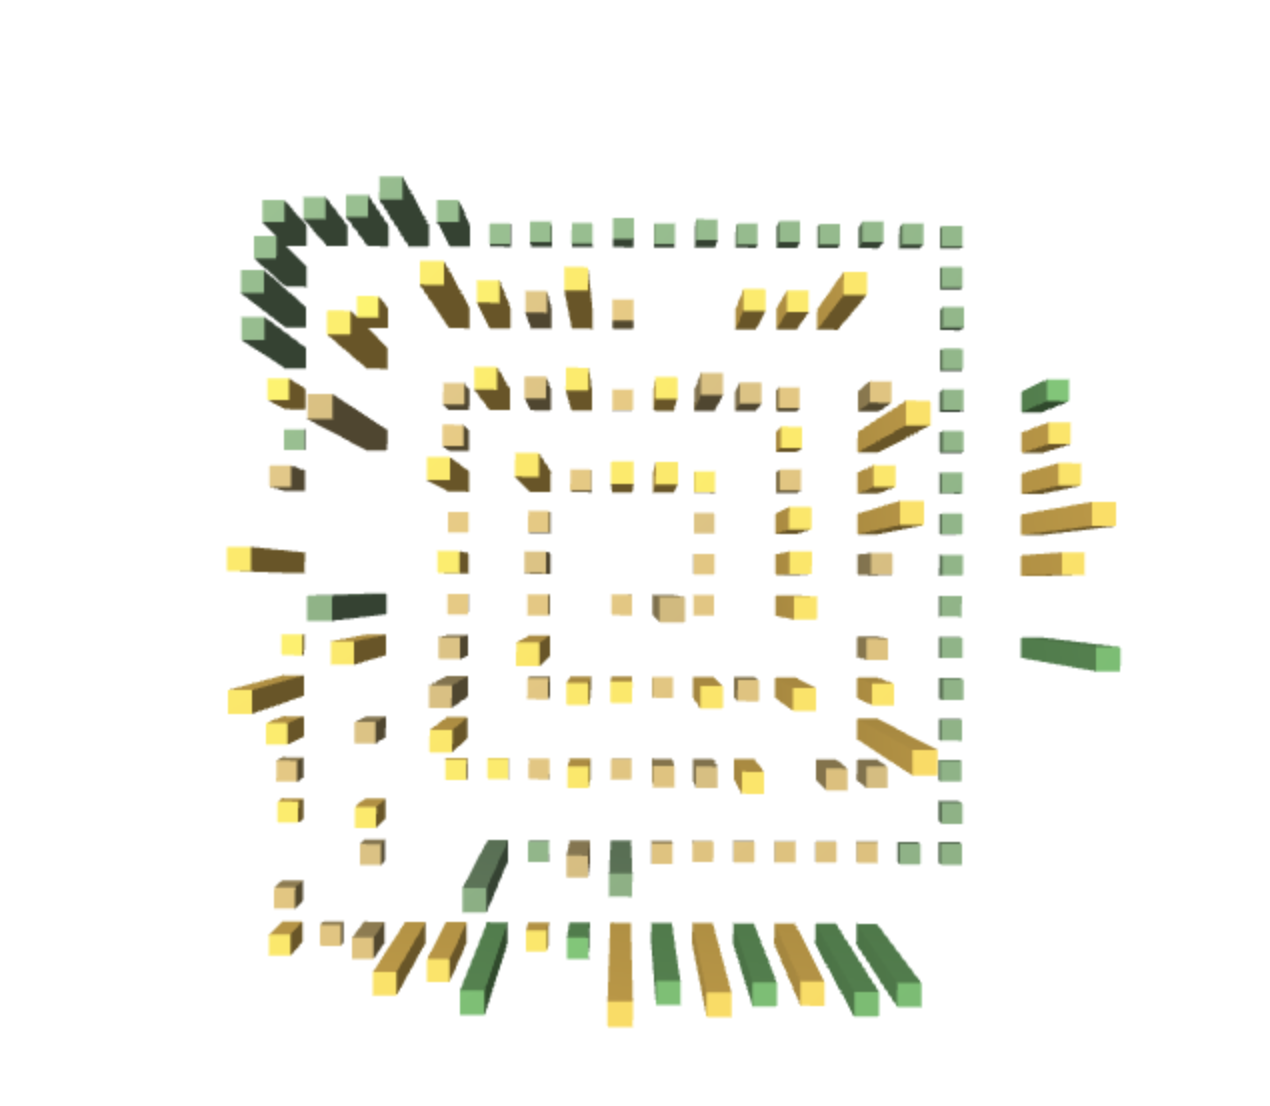
\includegraphics[width=\linewidth]{JetUML_V1S3.png}
        \caption{Month 3} \label{fig:JetUML_V1S3}
    \end{subfigure}\hspace*{\fill}
    \begin{subfigure}{0.48\textwidth}
    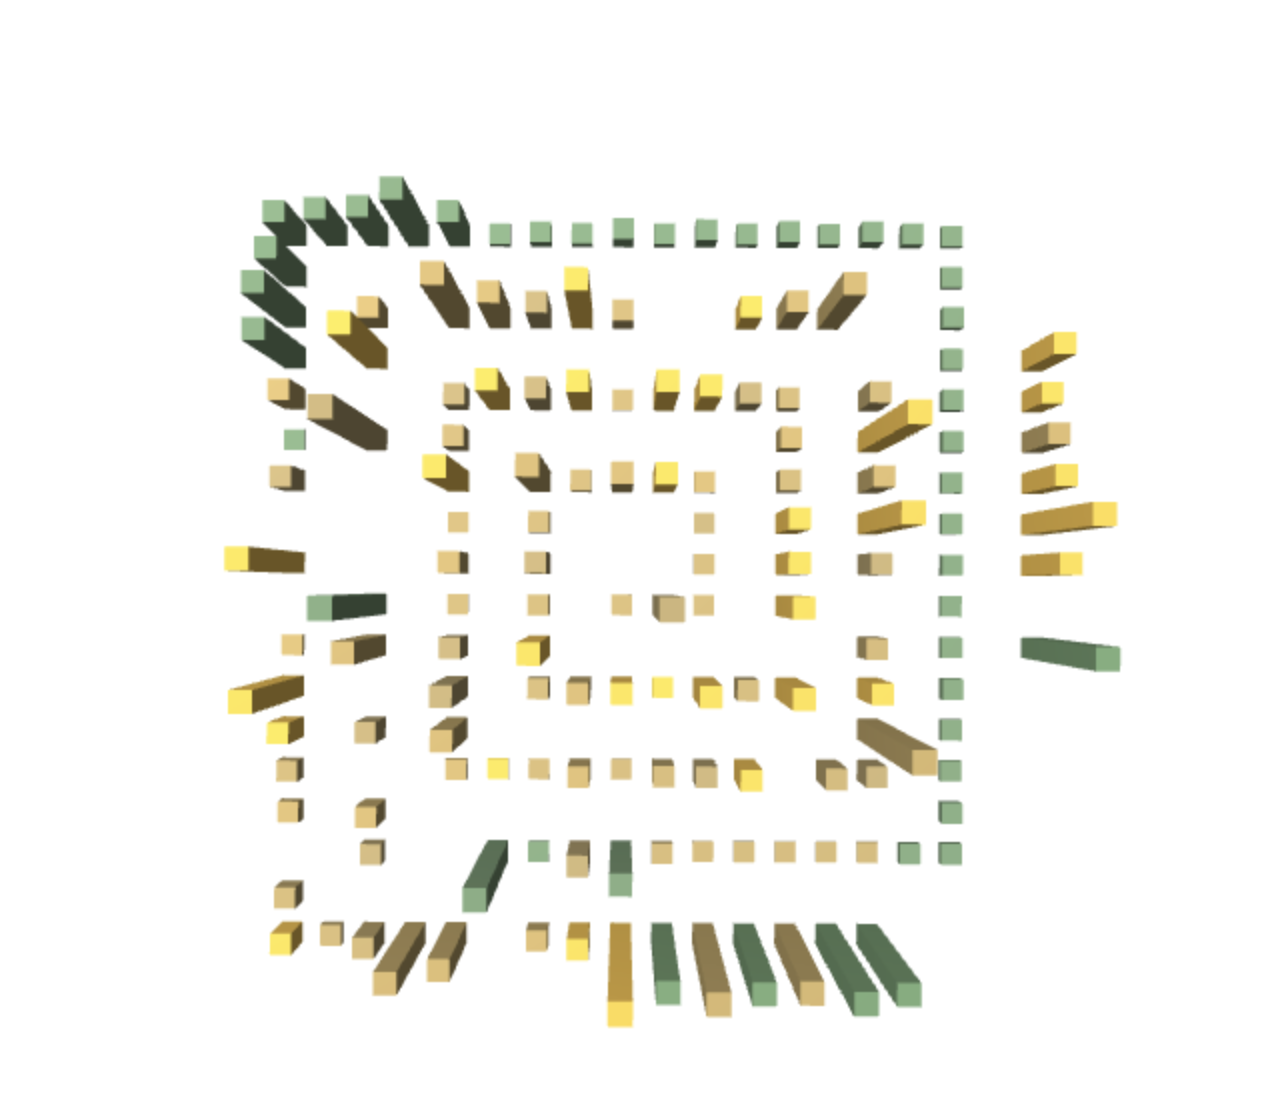
\includegraphics[width=\linewidth]{JetUML_V1S4.png}
    \caption{Month 4} \label{fig:JetUML_V1S4}
    \end{subfigure}
    
    \medskip
    \begin{subfigure}{0.48\textwidth}
        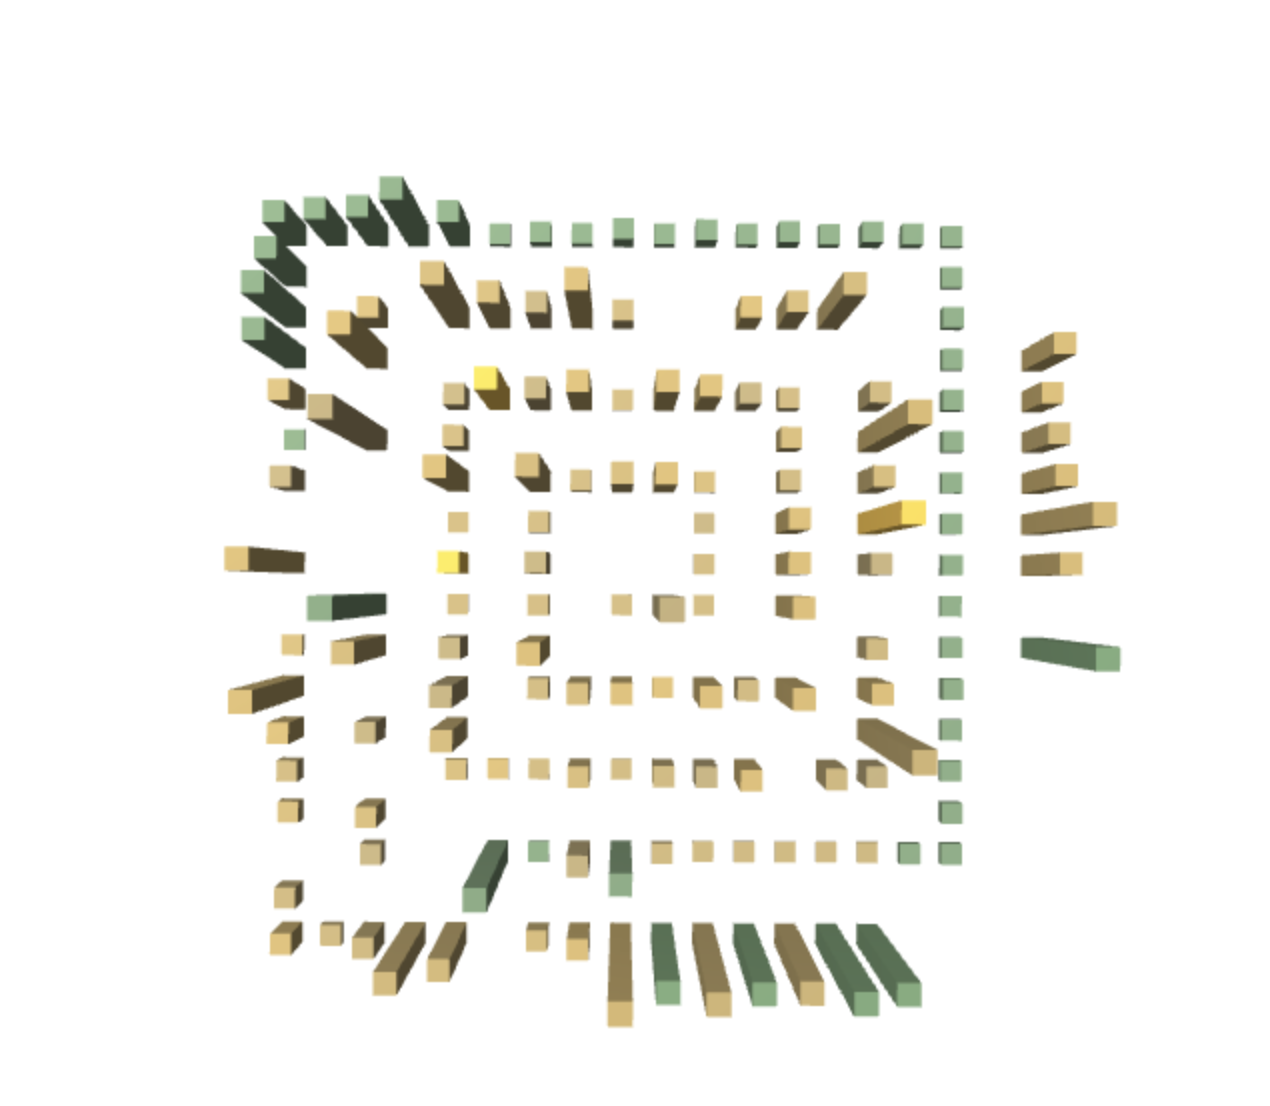
\includegraphics[width=\linewidth]{JetUML_V1S5.png}
        \caption{Month 5} \label{fig:JetUML_V1S5}
    \end{subfigure}\hspace*{\fill}
    \begin{subfigure}{0.48\textwidth}
        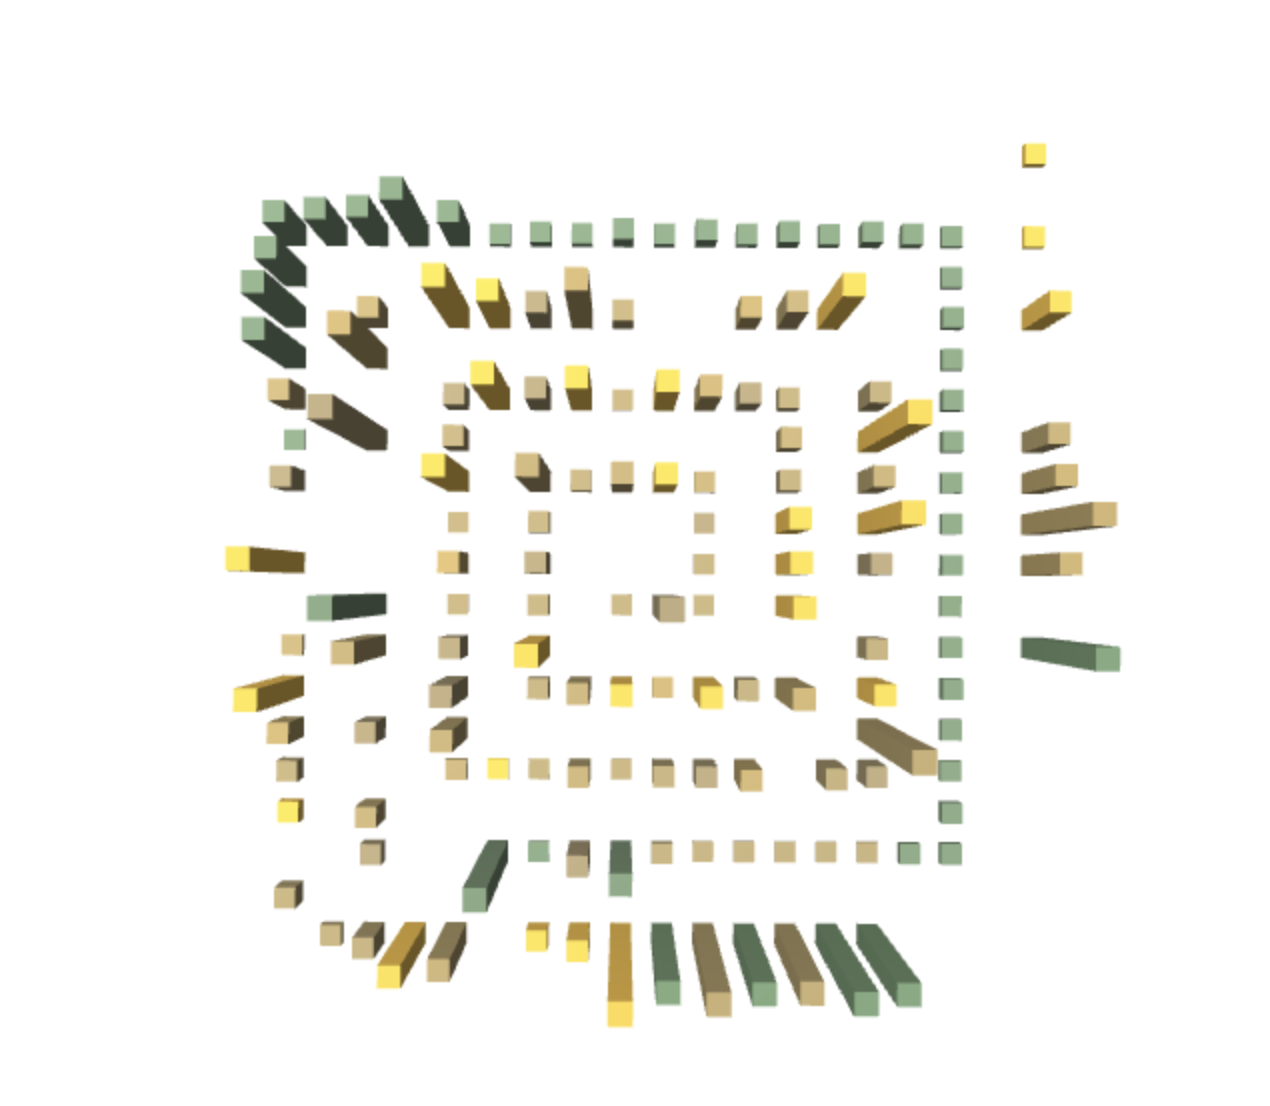
\includegraphics[width=\linewidth]{JetUML_V1S6.png}
        \caption{Month 6} \label{fig:JetUML_V1S6}
    \end{subfigure}
    
    \caption{First six month of the JetUML evolution.} 
    \label{fig:JetUML_V1}
\end{figure}
\clearpage
\section{JetUML 3}
\textbf{Goal of this visualization}
In this third and last visualization that we propose, the goal is to study the entire evolution of the system, with a focus on Java files. 
To do that, the use the shape and opacity property of a ViewFigure, to distinguish them among others. 
To display the evolution of the system we adopt a timestamp grouping strategy, with a timestamp of one year. 
Furthermore, we also use a timestamp strategy for the aging, with a total of ten steps and a time window of one month. This means that grey entities represent files that have not been received any update for the last 10 month from the time of the displayed AnimationFrame. 
\begin{itemize}
    \item \texttt{versionGroupingStrategy}: timestamp.
    \item \texttt{versionGroupingChunkSize}: 31'556'926 (1 year). 
    \item \texttt{colorPalette}: default.
    \item \texttt{agingGroupingStrategy}: timestamp.
    \item \texttt{agingStepSize}: 2'629'743 (1 month).
    \item \texttt{agingSteps}: 10 steps. 
    \item \texttt{mapperMetricName}: SLOC. 
    \item \texttt{fileTypeShape}: Java -> BOX, OTHERS -> SPHERE. 
    \item \texttt{fileTypeOpacity}: Java -> max, OTHERS -> low. 
\end{itemize}

\textbf{Results}
The whole evolution of JetUML is depicted in \autoref{fig:JetUML_V3}. As we notice, it is straightforward to distinguish java files from others because they have different shapes and other files are less opaque. After the first year of development, the state of the repository is shown in \autoref{fig:JetUML_V3S1}. We notice that all the Java files have more or less the same age. This means that all of them were updated after the second month because otherwise, they would be grey. The system grew at the end of the second year, shown in figure \autoref{fig:JetUML_V3S2} and now we can see some grey entities. Most of them are in the middle, meaning that the "core" files, or the files added before others, were not touched after the fourteenth month.  \autoref{fig:JetUML_V3S3} shows the state of the repository at the end of the third year. The system grew, and all the Java files were updated recently. Considering what we have seen in the first visualization, they had to change the path from all the Java files (\autoref{fig:JetUML_V0S8}). Perhaps this can be why all the entities were updated, and some ViewFigures are painted with the blue color. The fourth year of development, shown in  \autoref{fig:JetUML_V3S4} recorded a little activity in the first months because the system grew, and almost all the entities have a different color. However, it tends to be close to the base color, meaning they are old. 
\autoref{fig:JetUML_V3S5},  \autoref{fig:JetUML_V3S6} and  \autoref{fig:JetUML_V3S7} shows how the system evolved through the fifth, sixth and seventh year. The fifth year recorded an intense activity compared to what we saw in the fourth year. Lots of files were added, and most of the classes of the system were modified. Moreover, the system's center is slowly disappearing, meaning that new ones have replaced old Java files. In the sixth and seventh years, non-Java files were added, and some Java classes were updated outside the system's core. Finally, the last year, represented by \autoref{fig:JetUML_V3S8}, did not record such a huge activity on the system. It became inactive since almost all the entities are grey, meaning that these files were not touched in the last ten months of evolution. However, in this frame, the two tallest entities of the system appeared. This means that in this last year, two java files were added (they were not present the year before) and rapidly became the biggest files in the repository.  
\bigbreak
\textbf{Conclusion}
With this visualization, we have seen JetUML from another point of view. The year visualization works very well with systems like JetUML with a comprehensive history. In fact, with just 8 AnimationFrames, we can infer when the development process was more intense in the past. 
\bigbreak
\textbf{Video}
We packed in a video the visualization that we presented with auditive support. The video is available at \url{https://workInProgress.com}

\begin{figure}[ht]
    \begin{subfigure}{0.50\textwidth}
        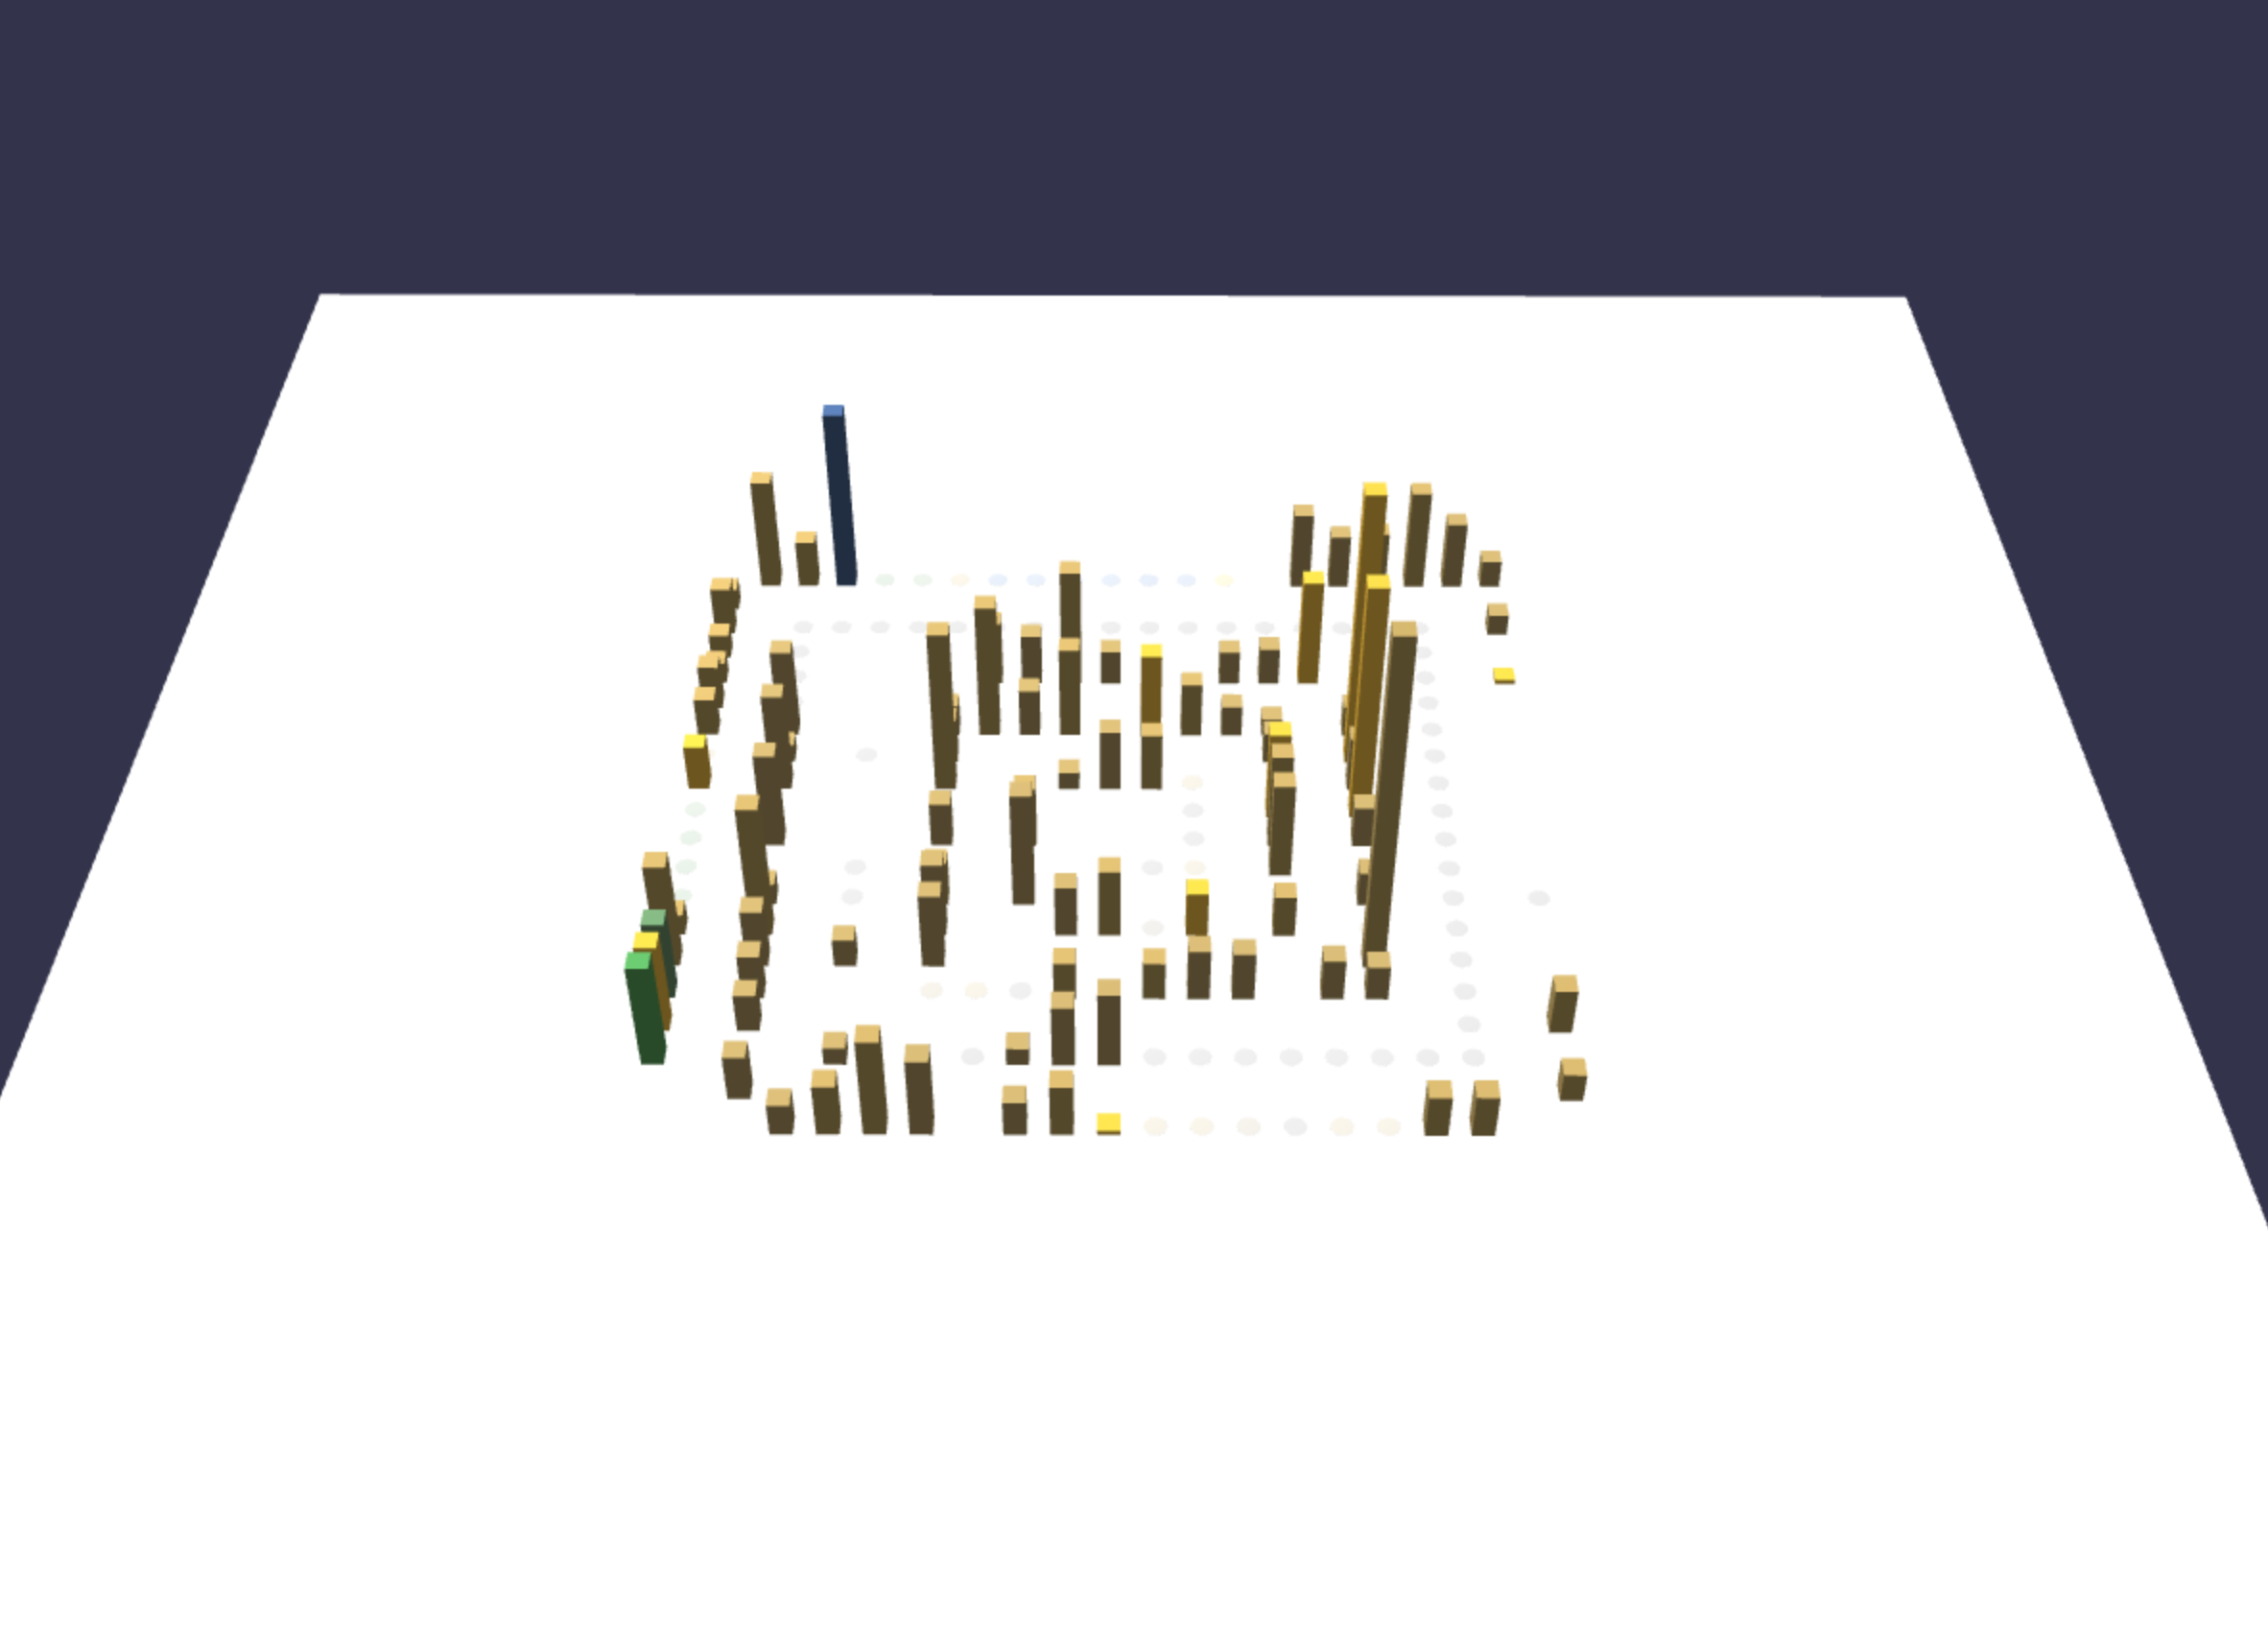
\includegraphics[width=\linewidth]{JetUML_V3S1.png}
        \caption{Year 1} 
        \label{fig:JetUML_V3S1}
    \end{subfigure}\hspace*{\fill}
    \begin{subfigure}{0.50\textwidth}
        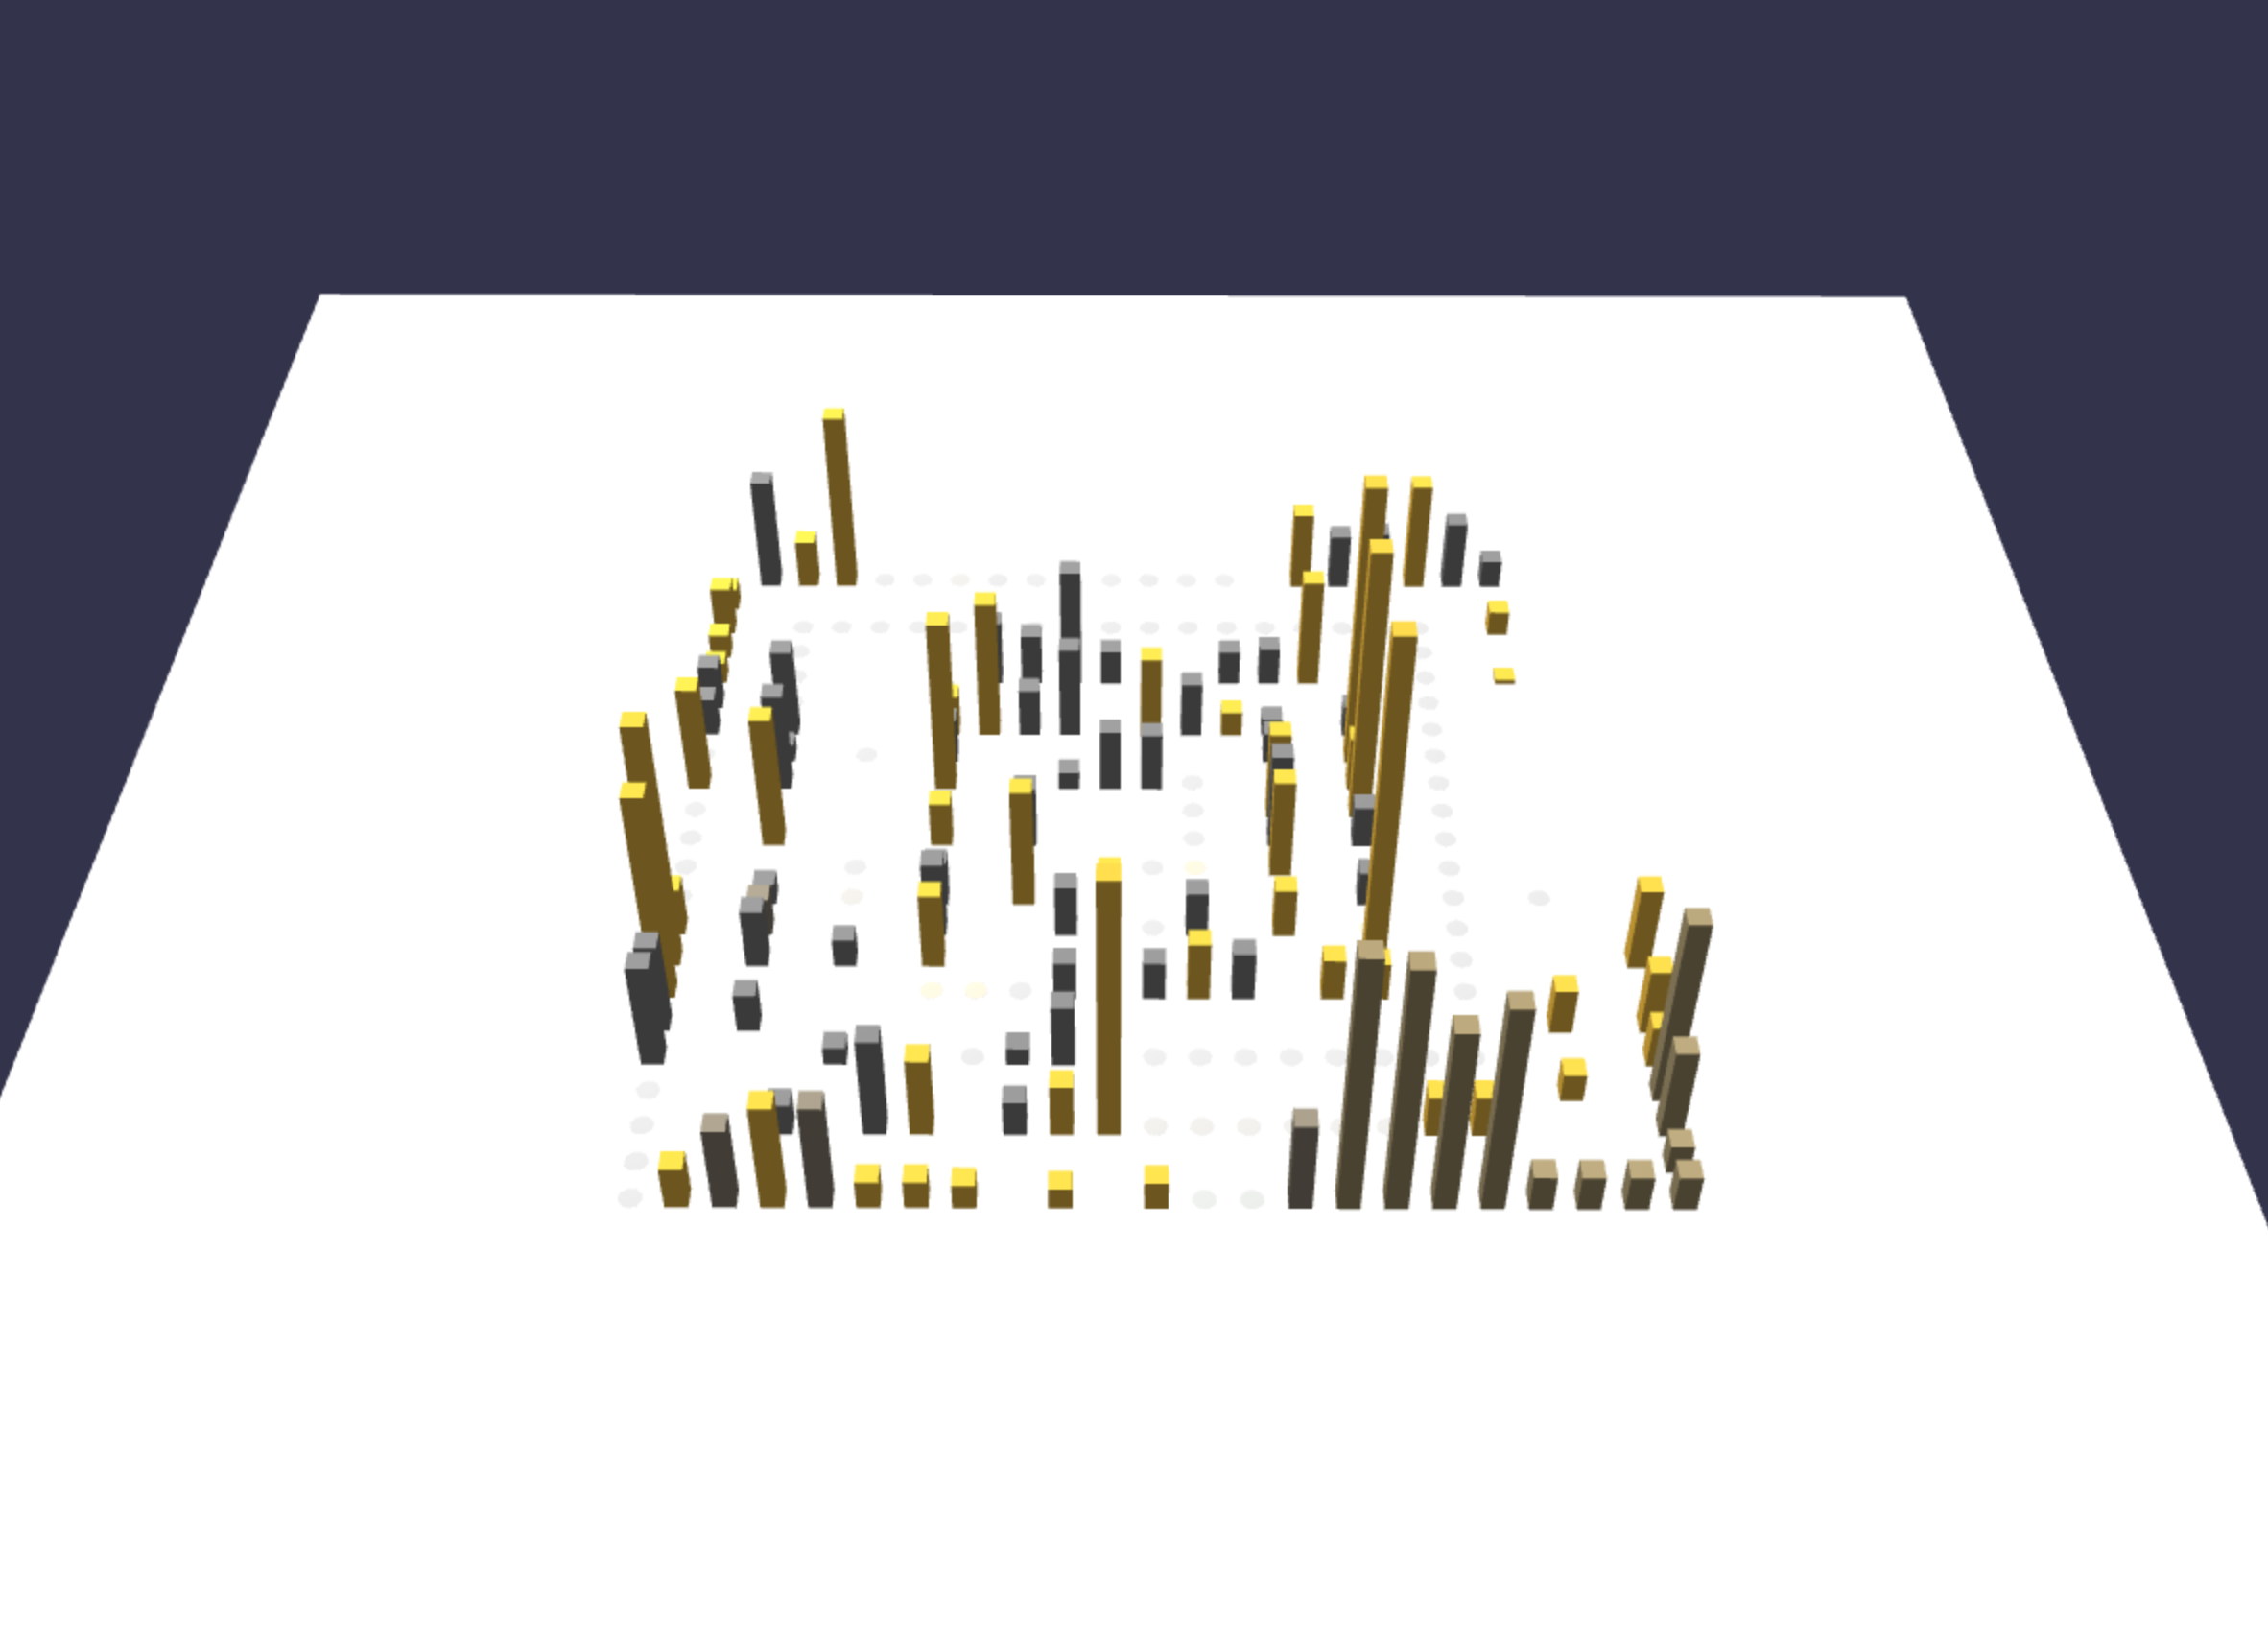
\includegraphics[width=\linewidth]{JetUML_V3S2.png}
        \caption{Year 2} 
        \label{fig:JetUML_V3S2}
    \end{subfigure}
    
    \medskip
    \begin{subfigure}{0.48\textwidth}
        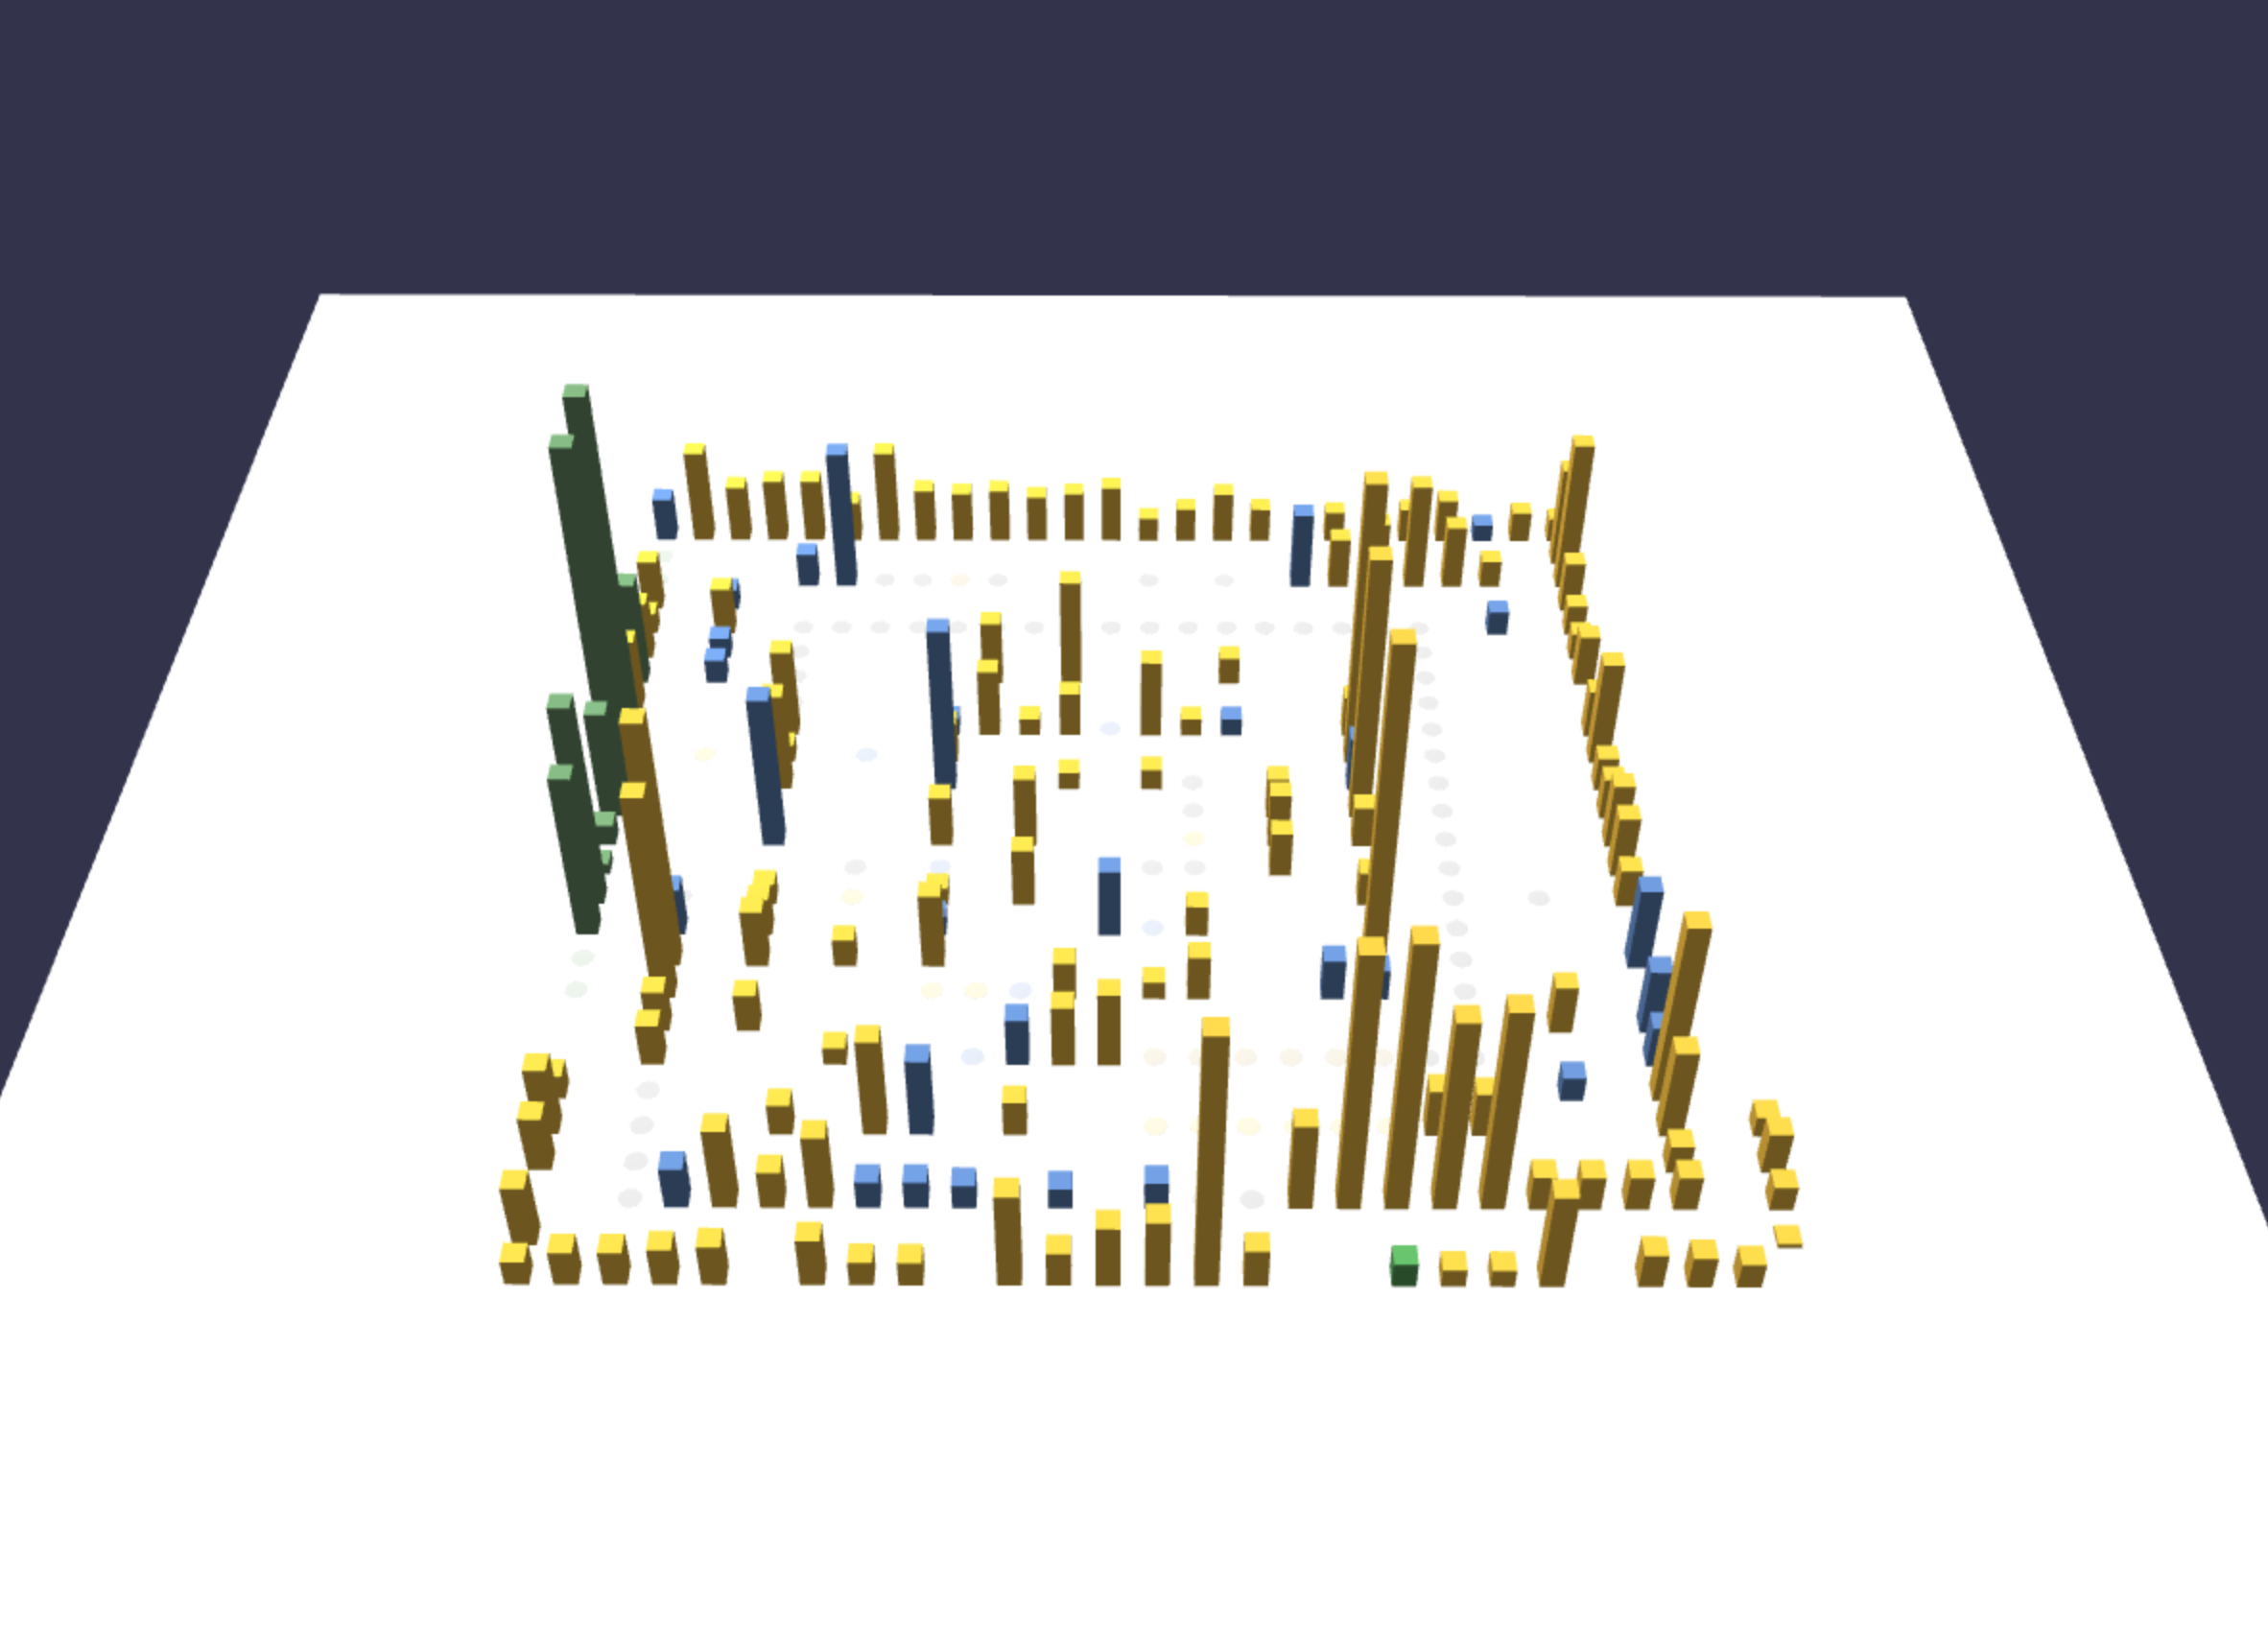
\includegraphics[width=\linewidth]{JetUML_V3S3.png}
        \caption{Year 3} 
        \label{fig:JetUML_V3S3}
    \end{subfigure}\hspace*{\fill}
    \begin{subfigure}{0.48\textwidth}
        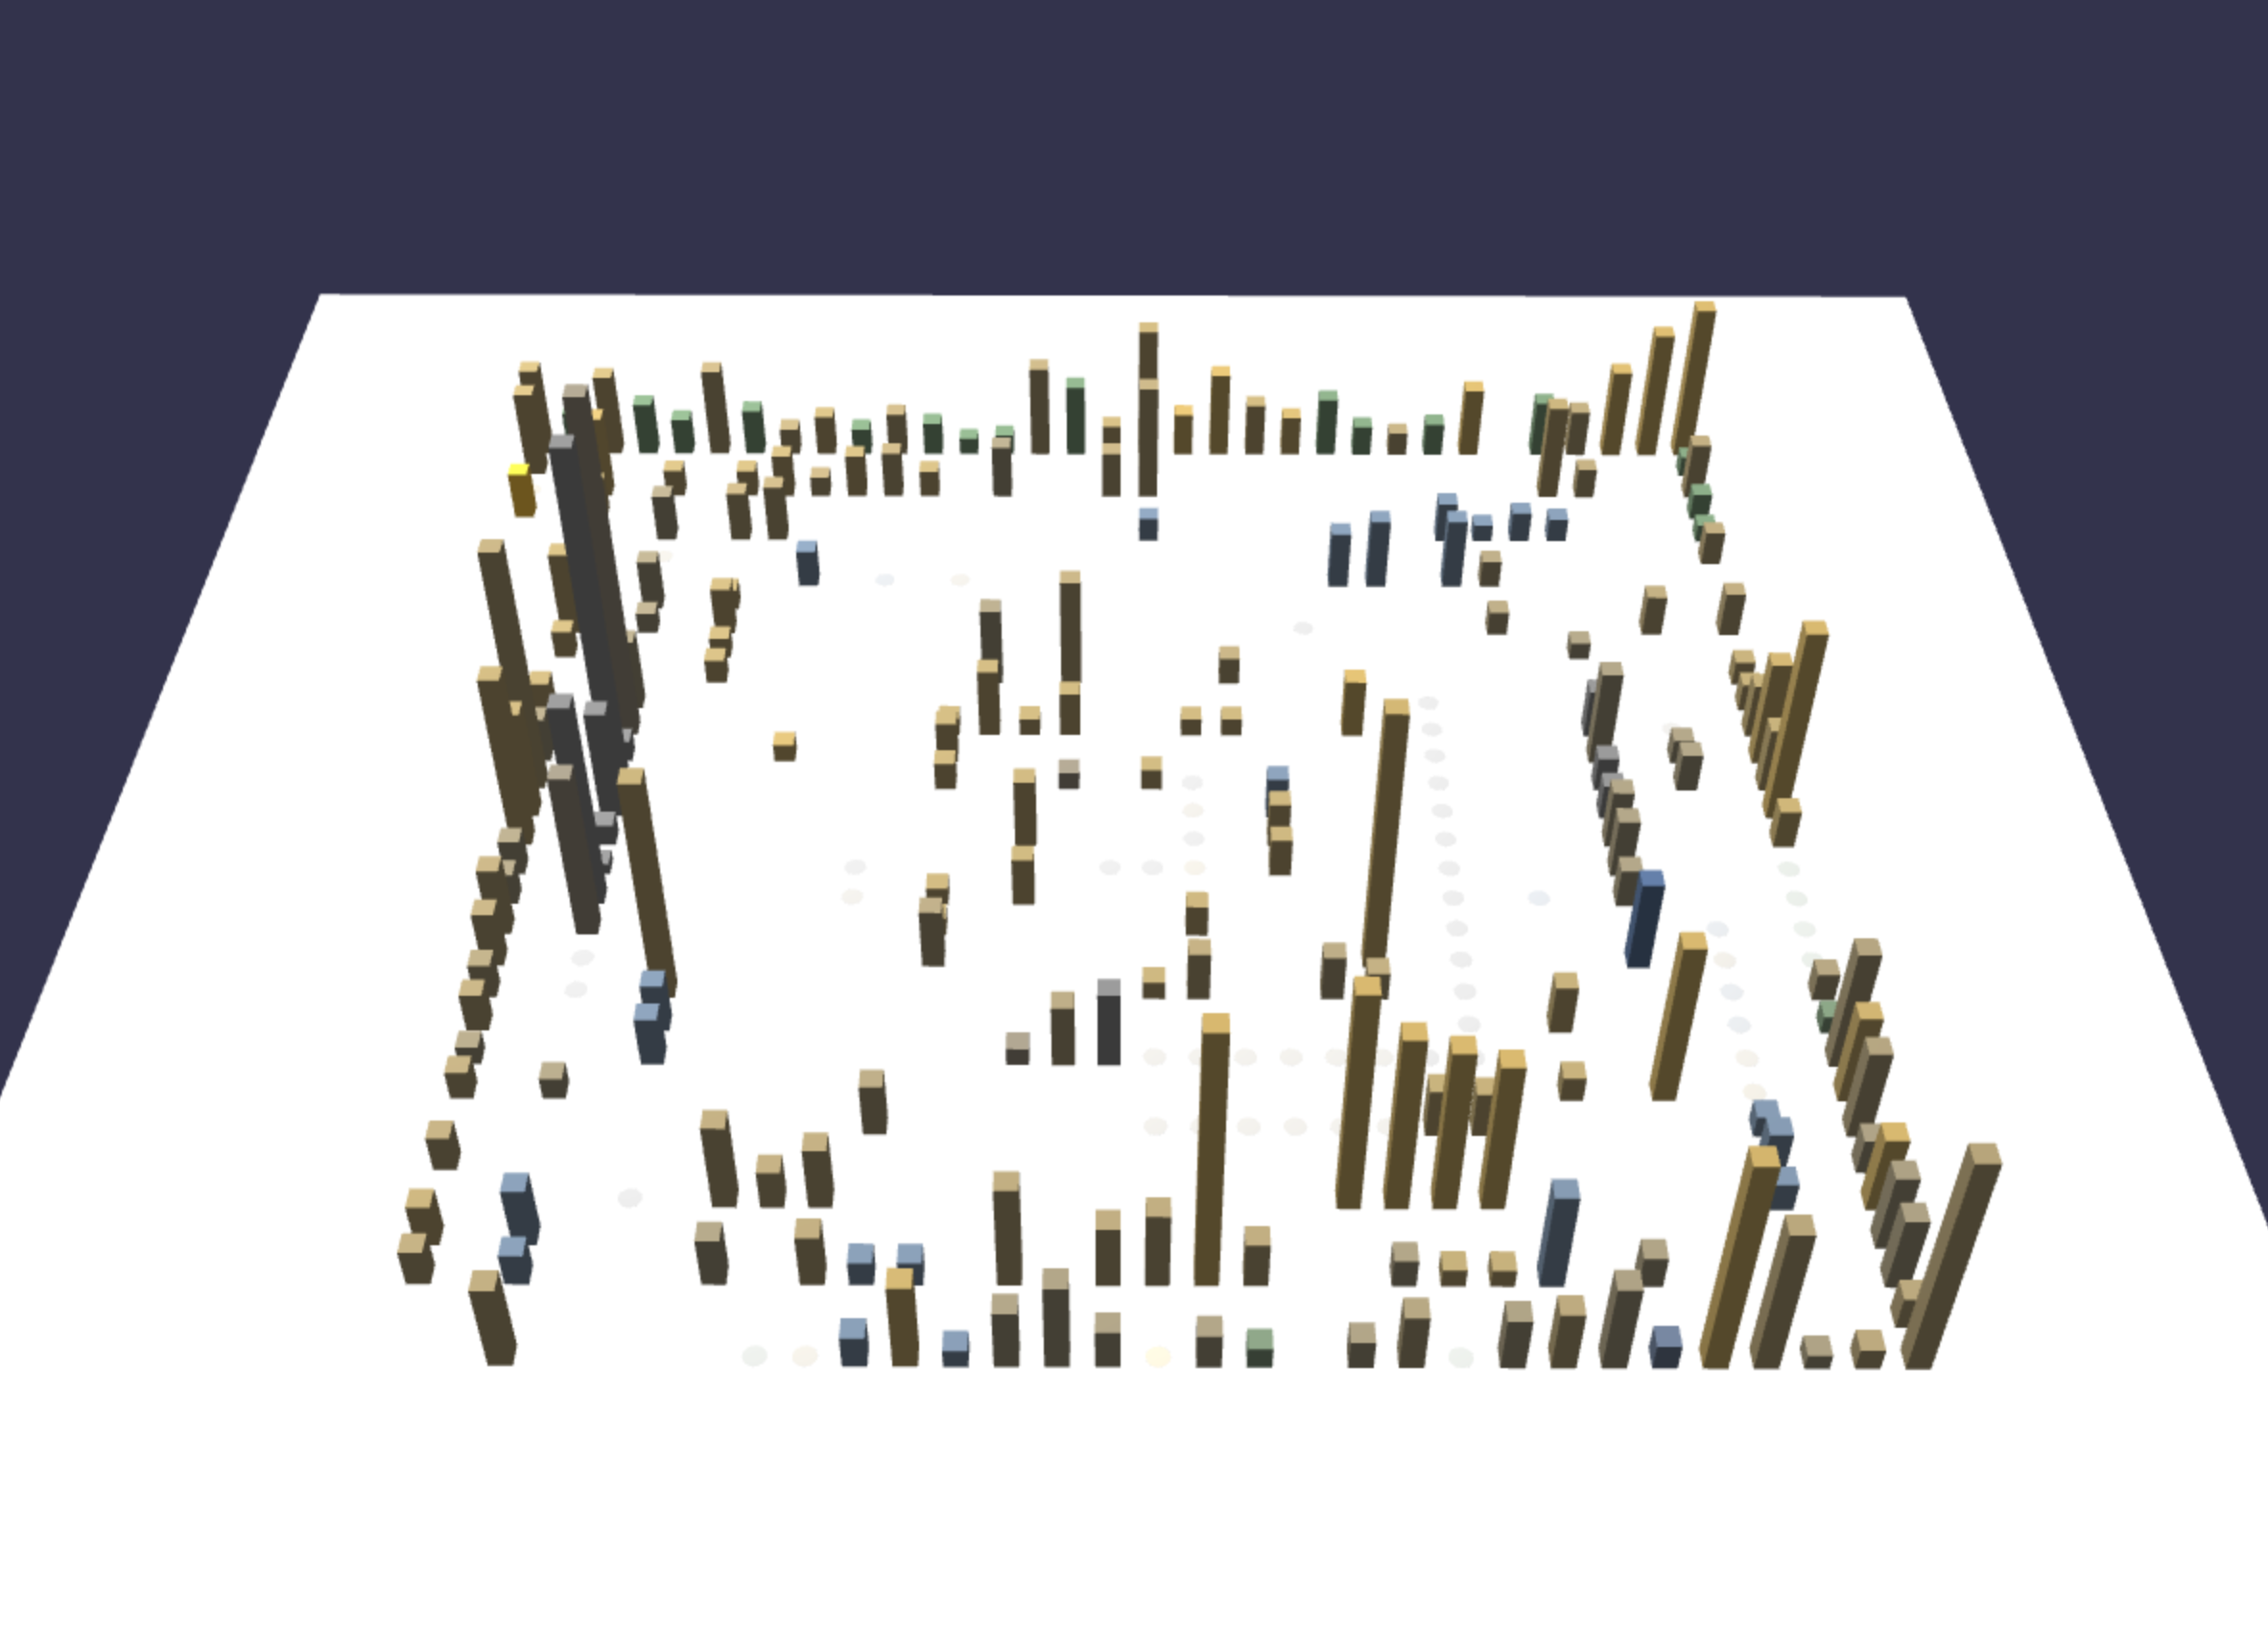
\includegraphics[width=\linewidth]{JetUML_V3S4.png}
        \caption{Year 4} 
        \label{fig:JetUML_V3S4}
    \end{subfigure}
        
    \caption{Evolution of JetUML} 
    \label{fig:JetUML_V3}
\end{figure}

\begin{figure}[h!]    \ContinuedFloat
    \begin{subfigure}{0.48\textwidth}
        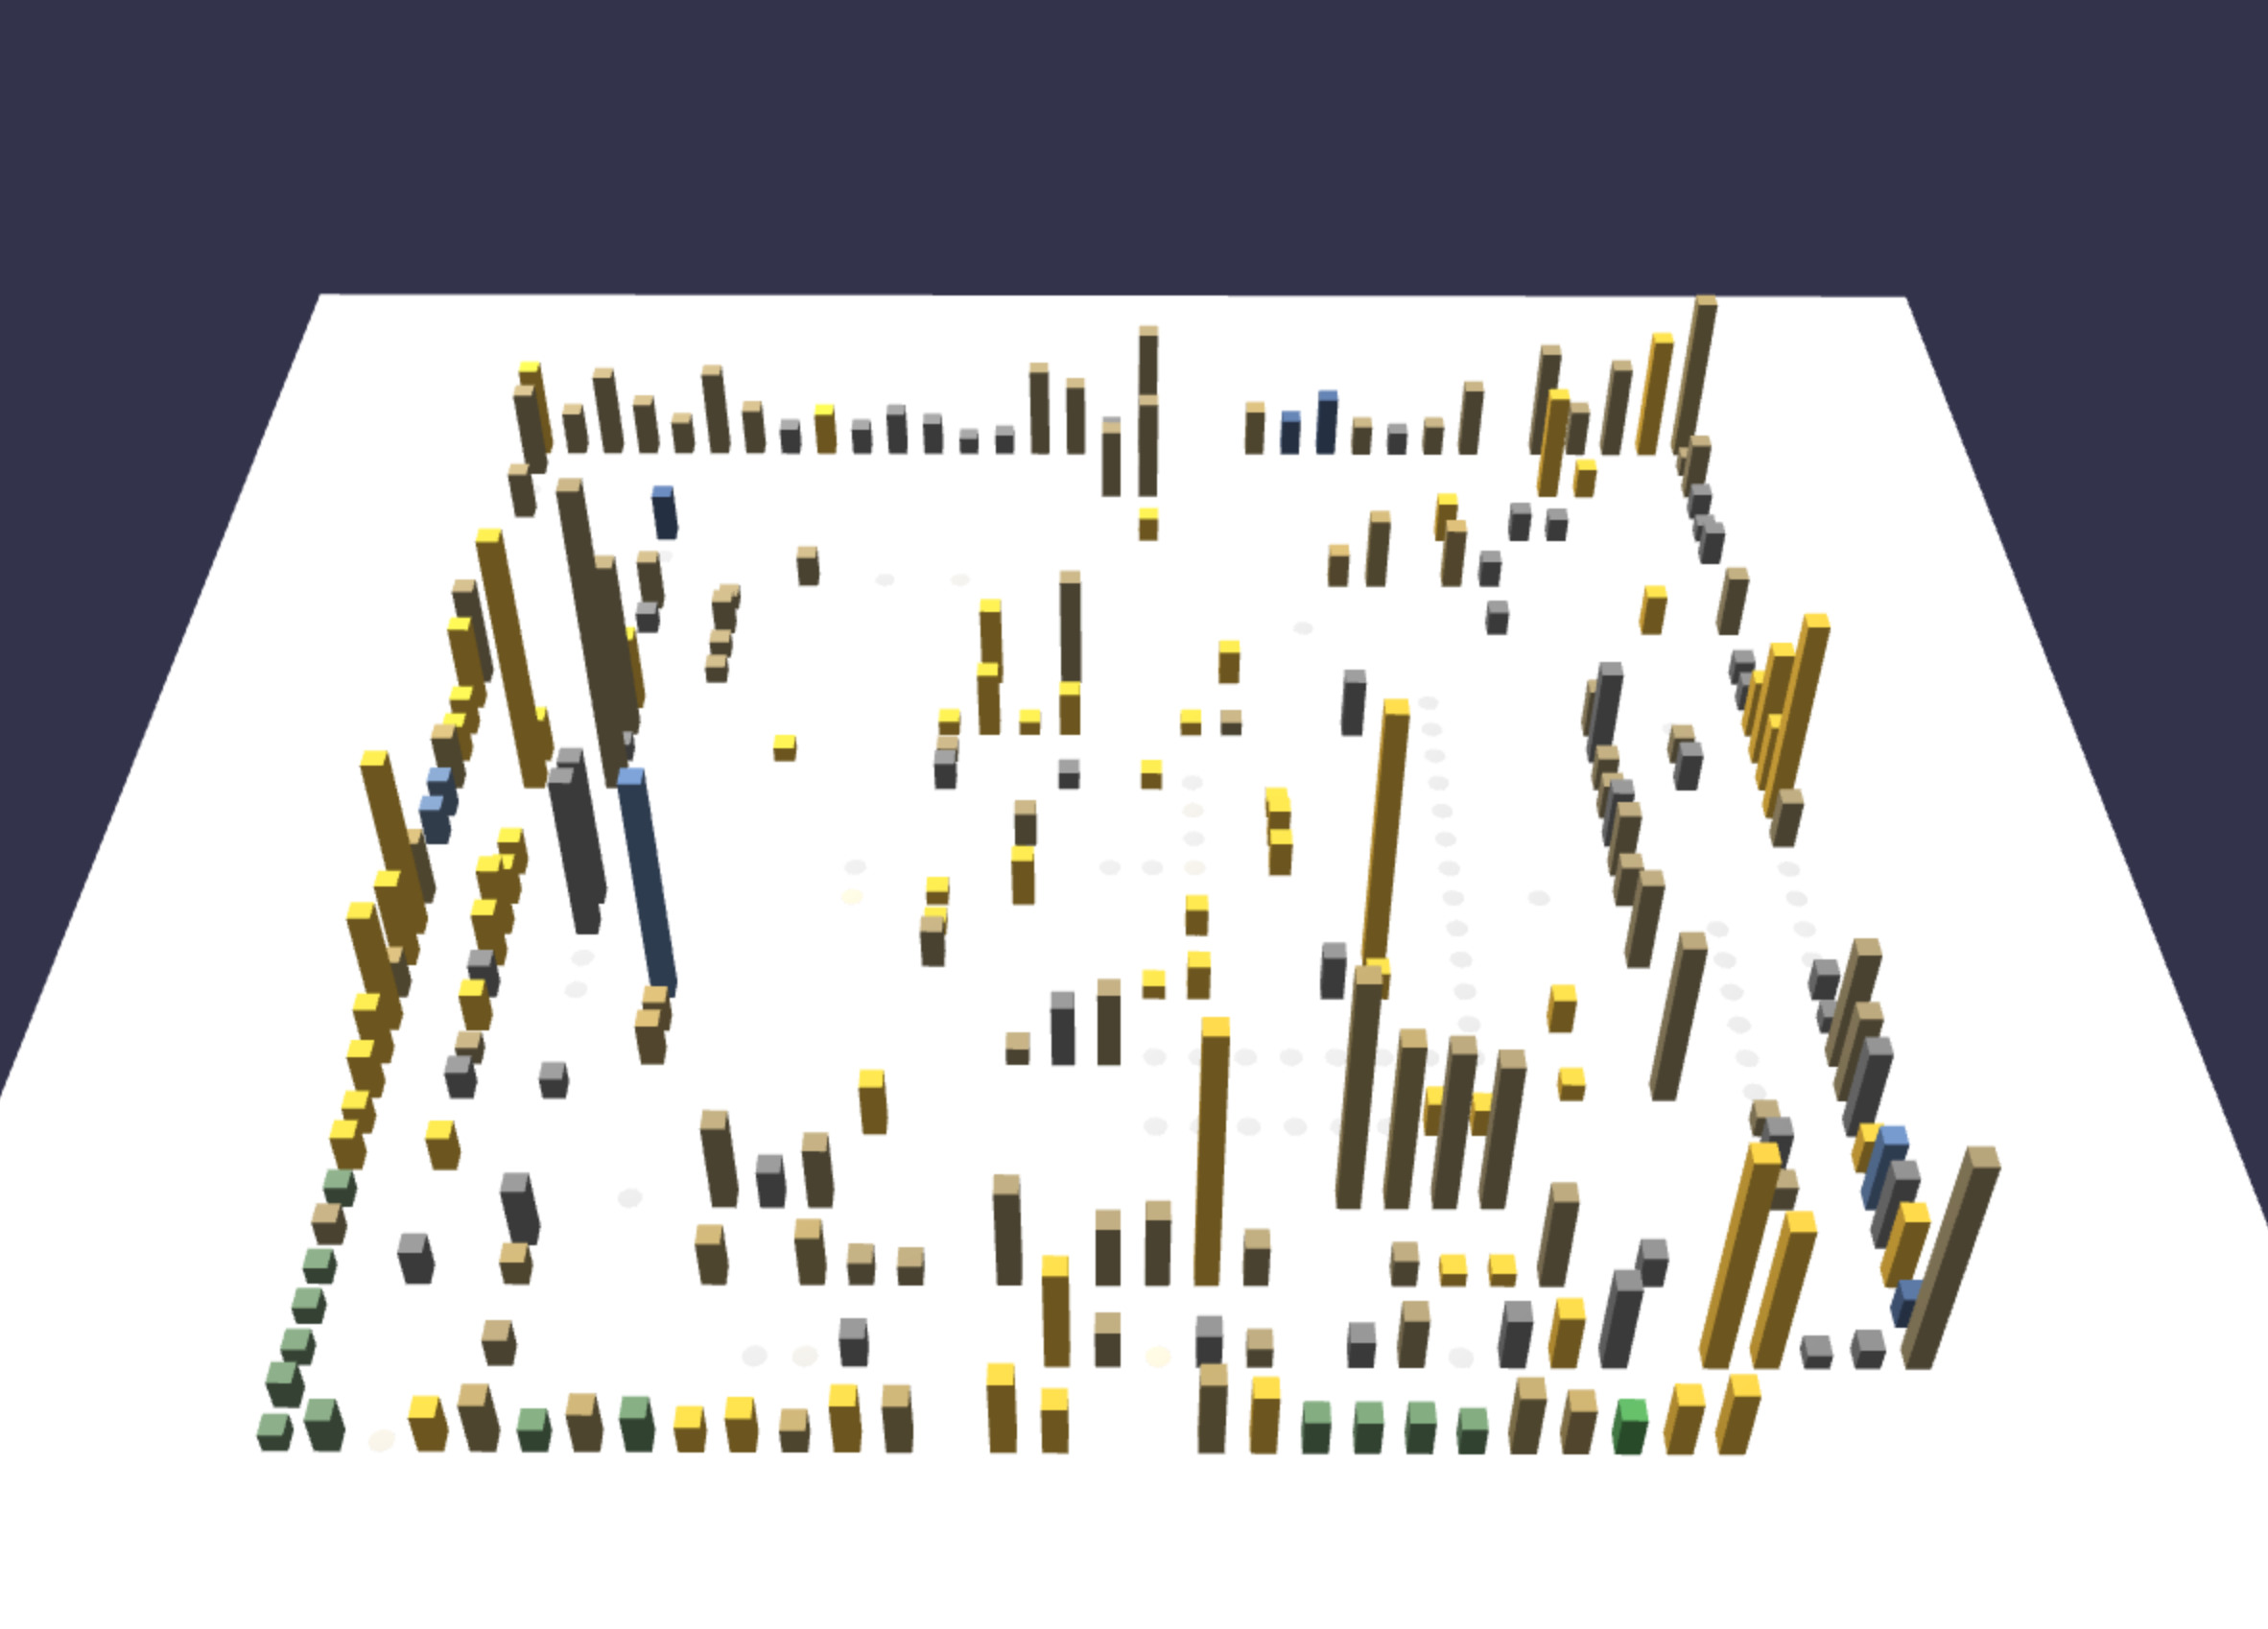
\includegraphics[width=\linewidth]{JetUML_V3S5.png}
        \caption{Year 5} 
        \label{fig:JetUML_V3S5}
    \end{subfigure}\hspace*{\fill}
    \begin{subfigure}{0.48\textwidth}
        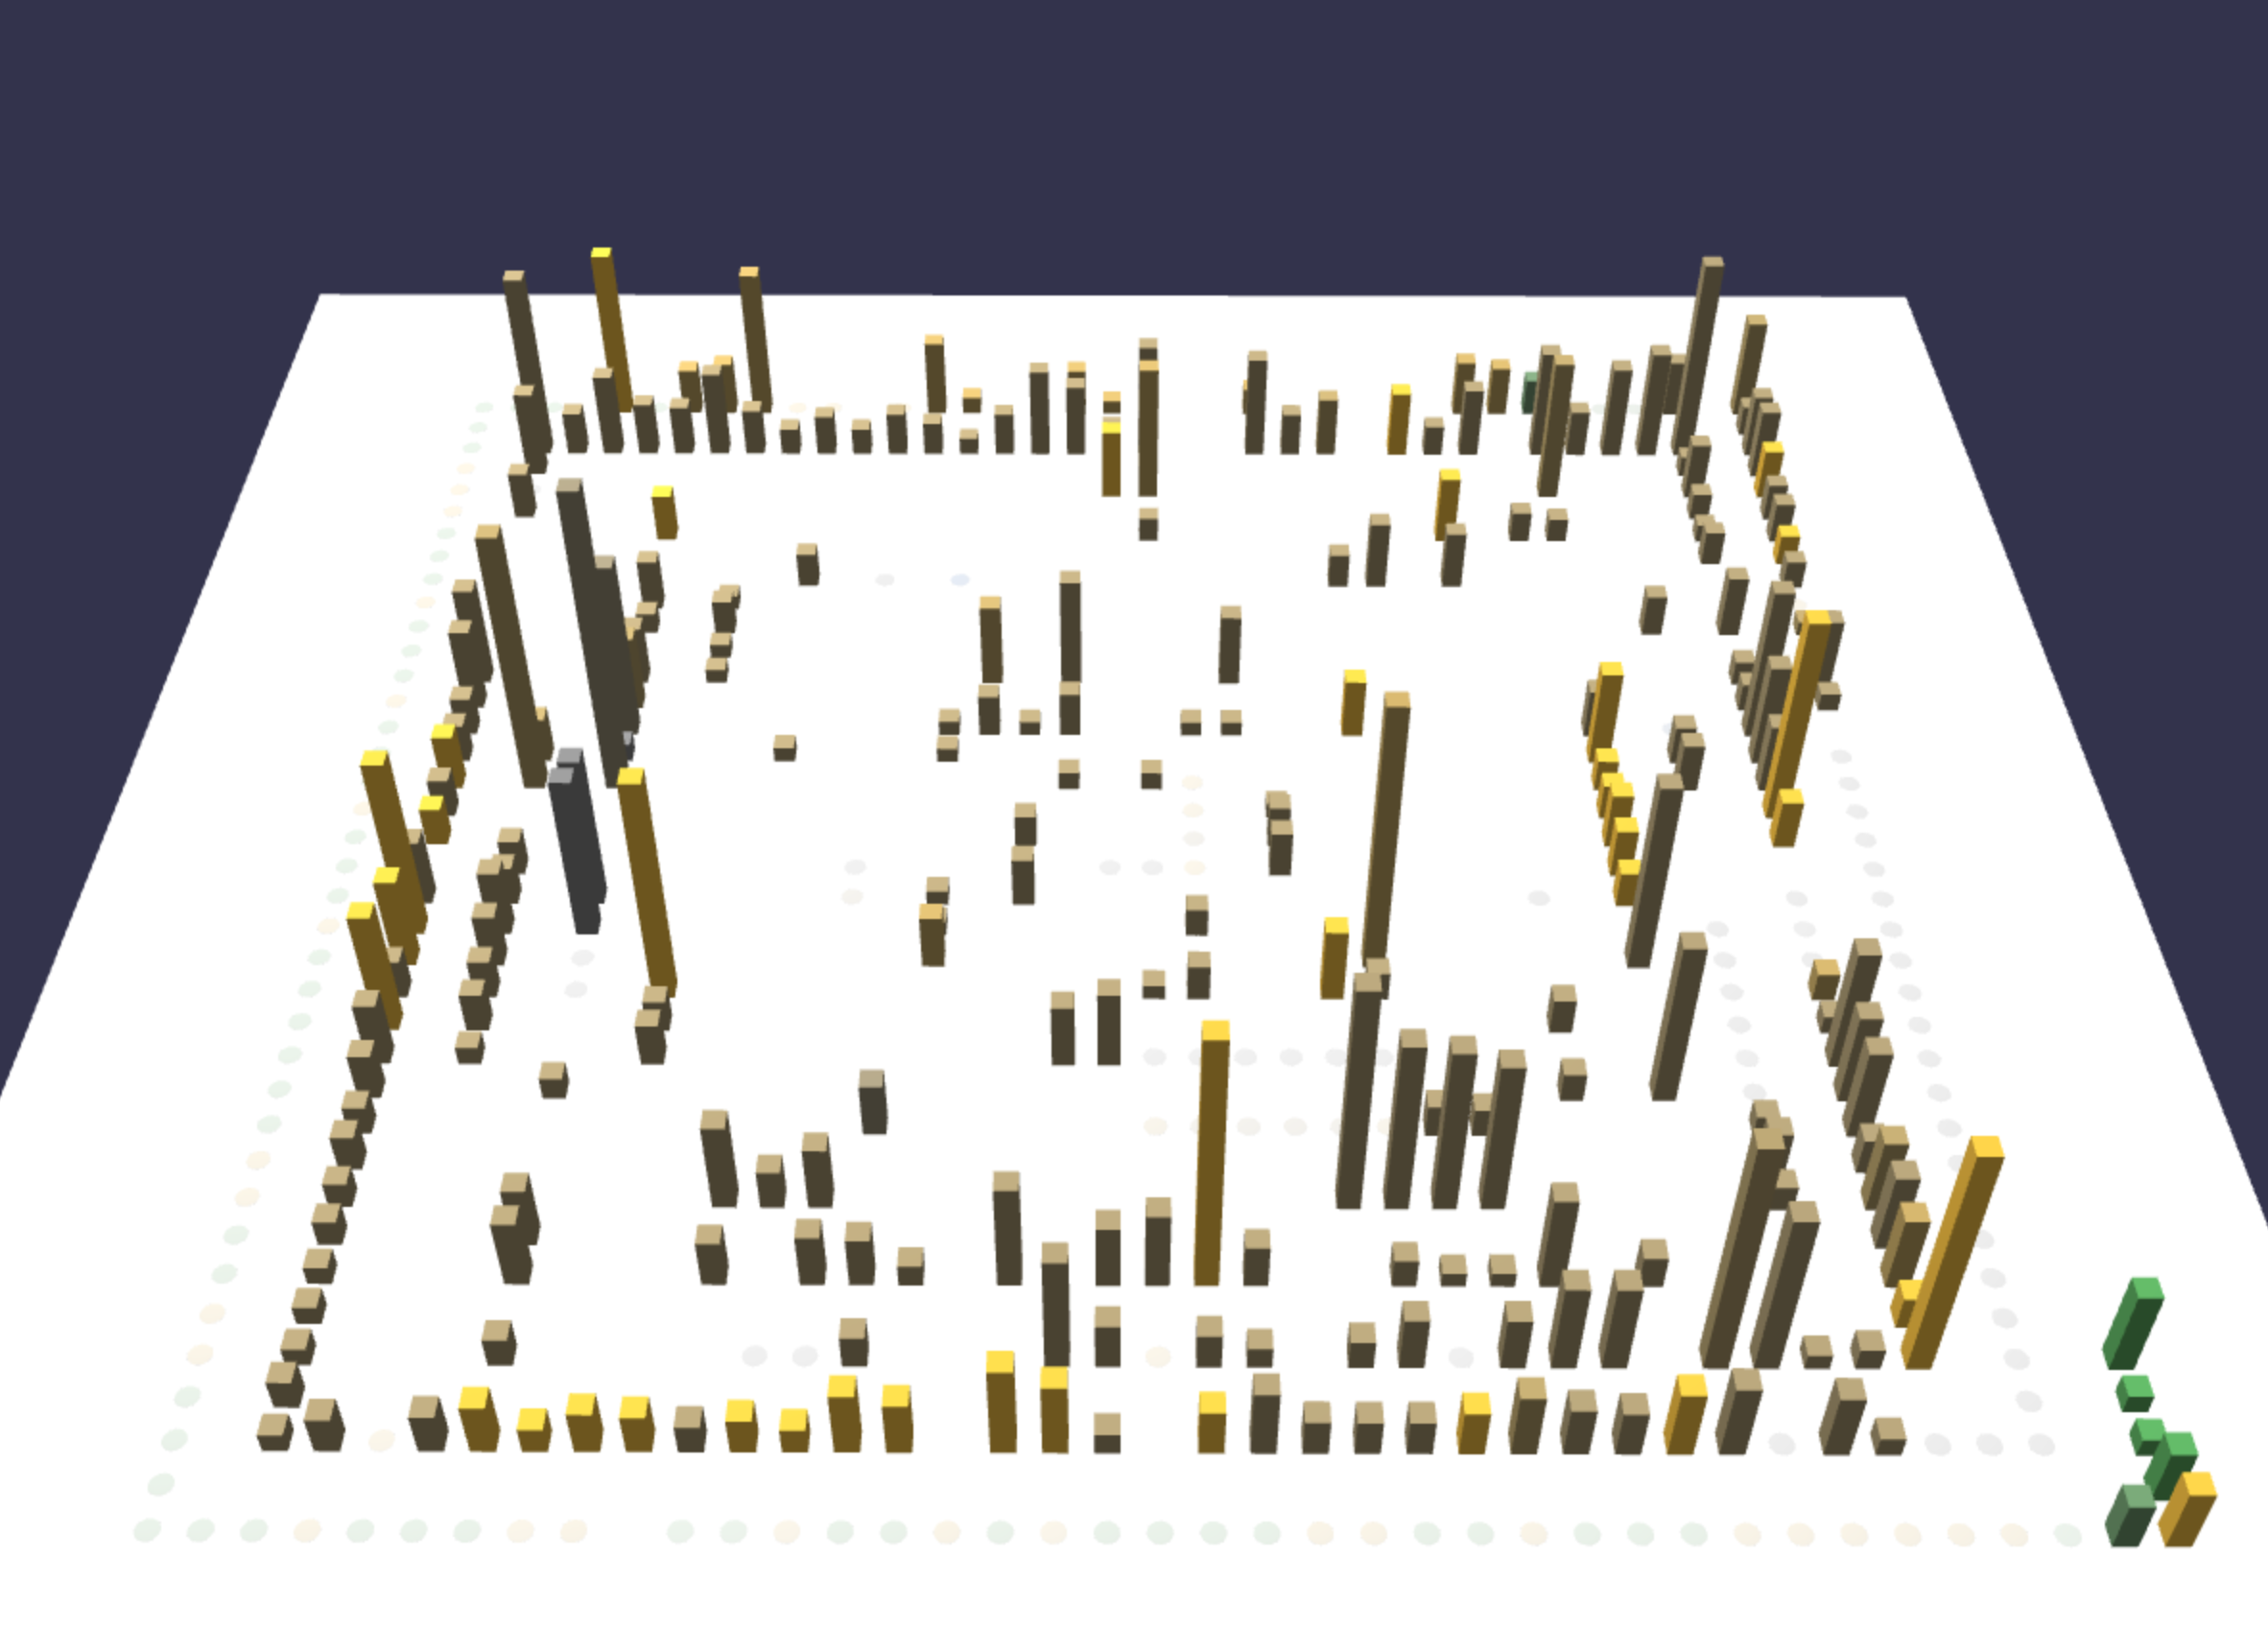
\includegraphics[width=\linewidth]{JetUML_V3S6.png}
        \caption{Year 6} 
        \label{fig:JetUML_V3S6}
    \end{subfigure}

    \medskip
    \begin{subfigure}{0.48\textwidth}
        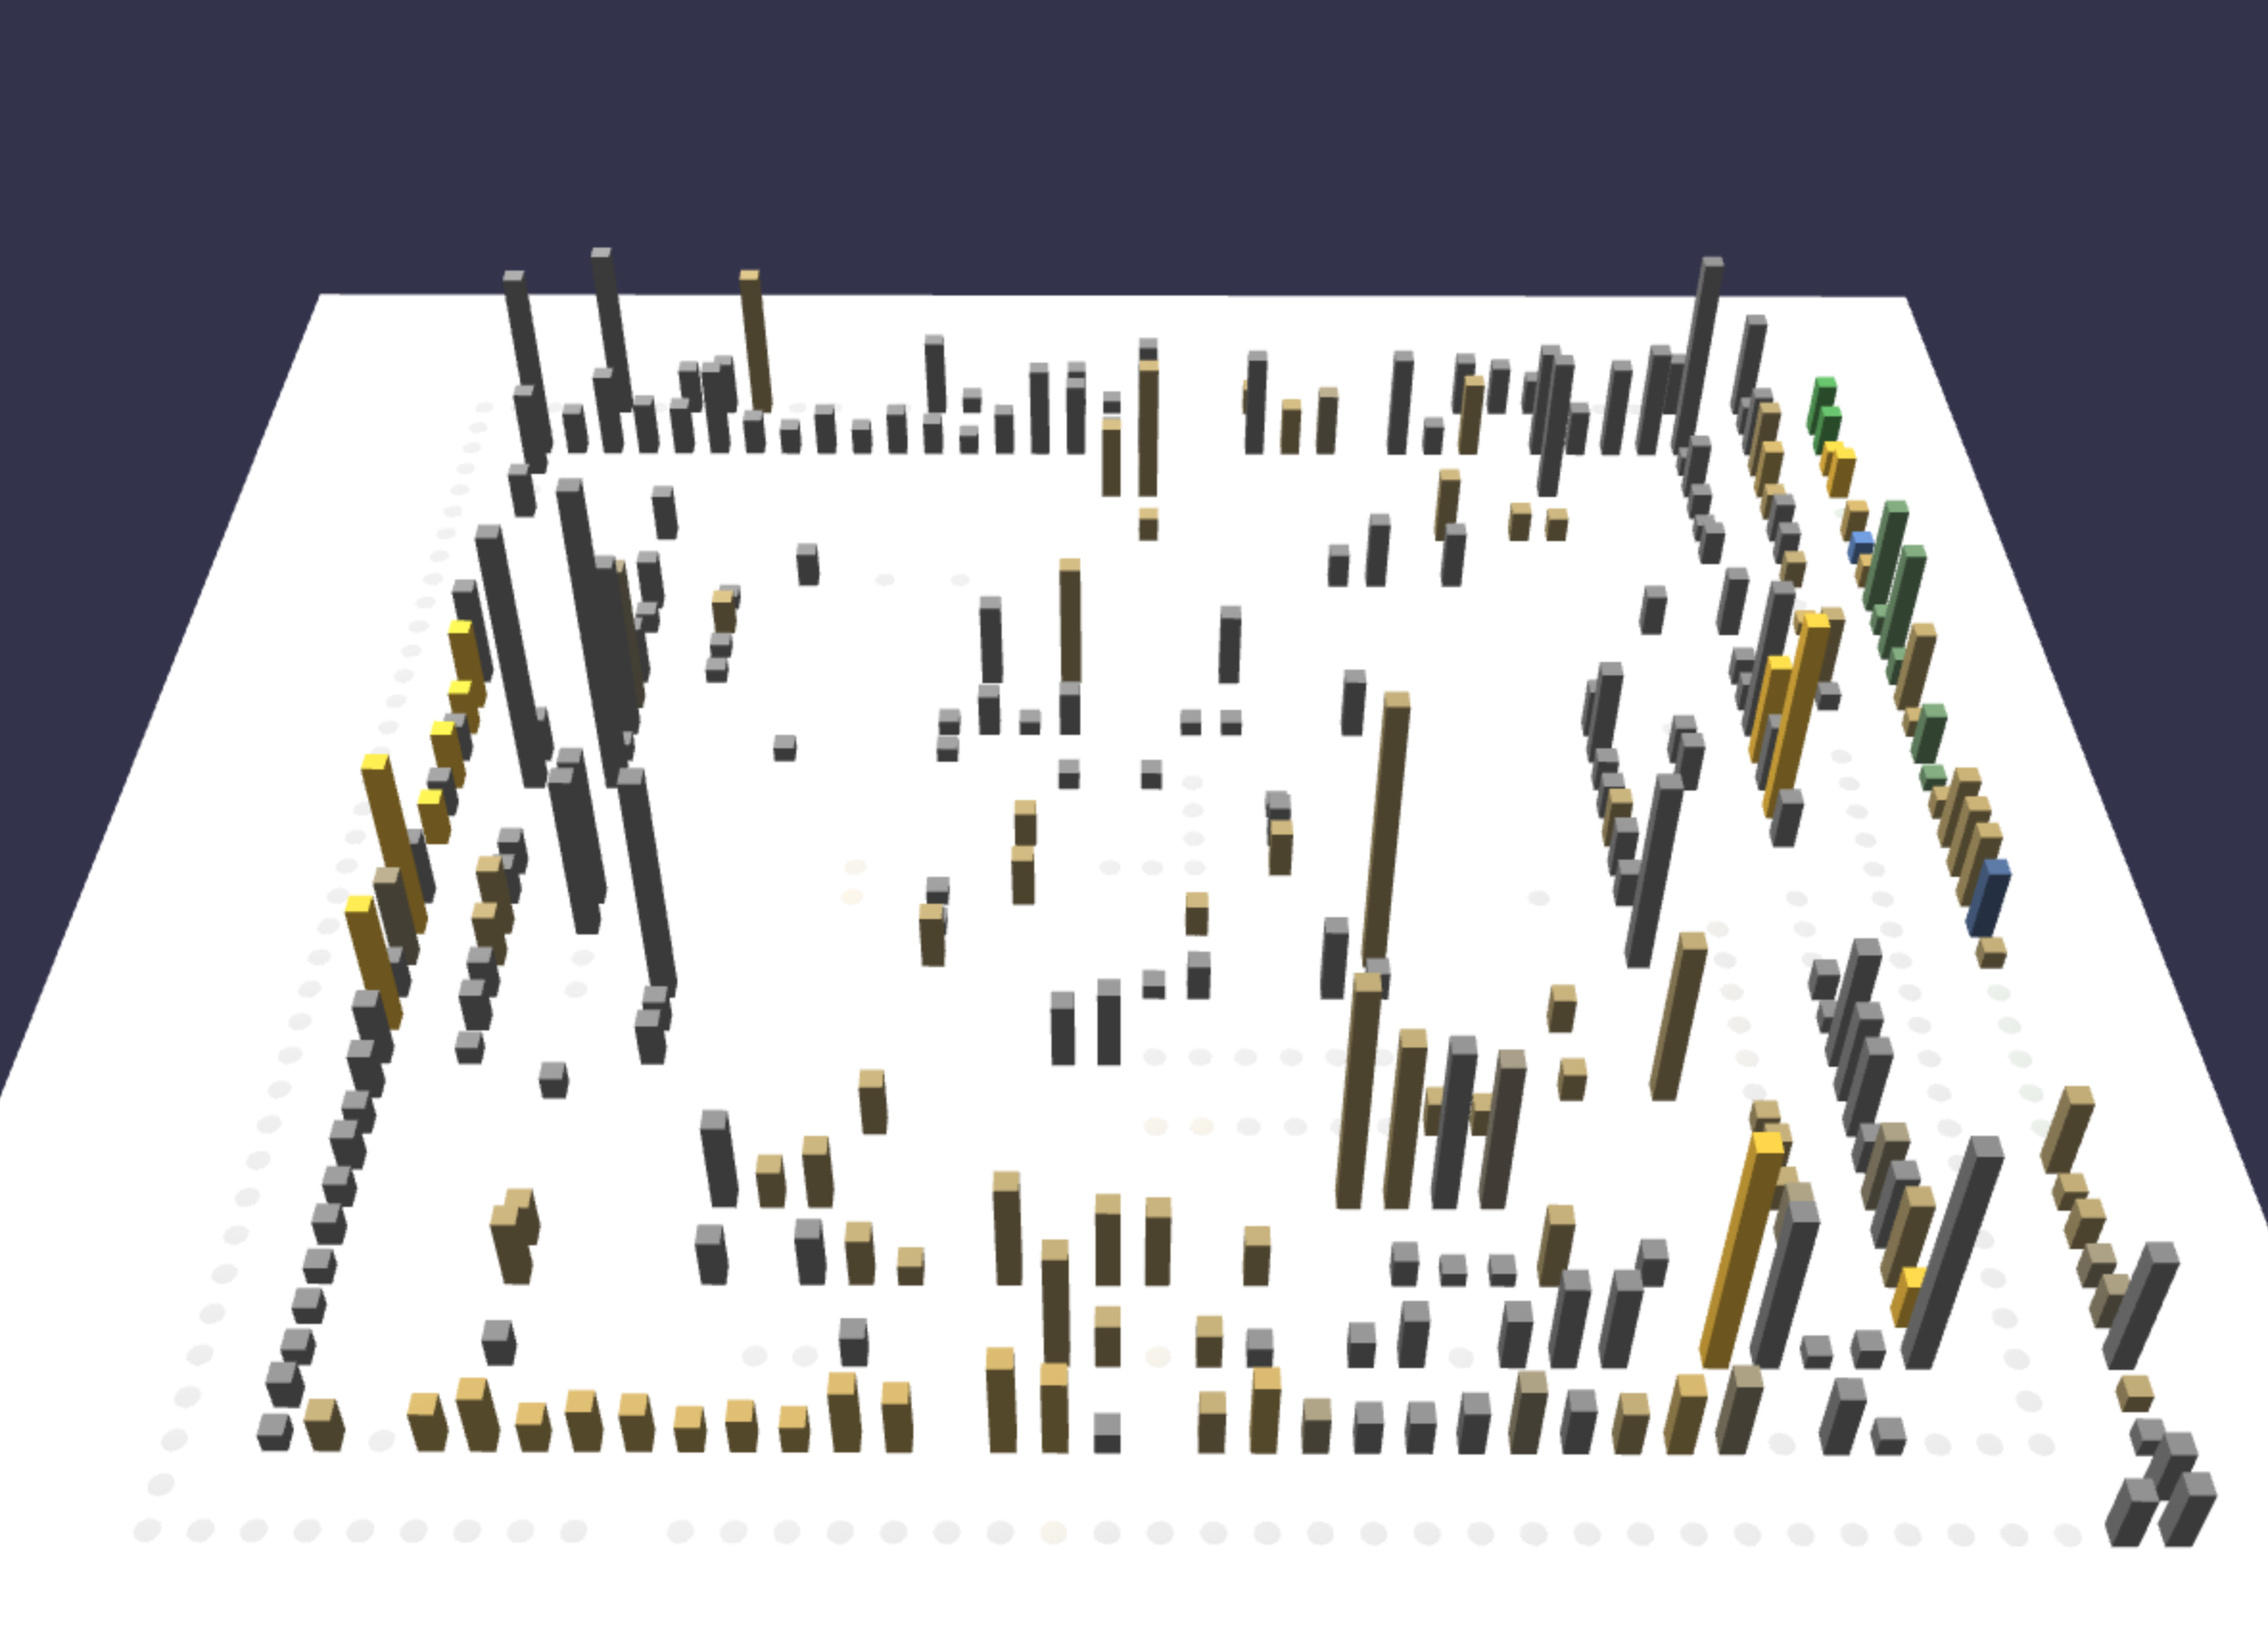
\includegraphics[width=\linewidth]{JetUML_V3S7.png}
        \caption{Year 7} 
        \label{fig:JetUML_V3S7}
    \end{subfigure}\hspace*{\fill}
    \begin{subfigure}{0.48\textwidth}
        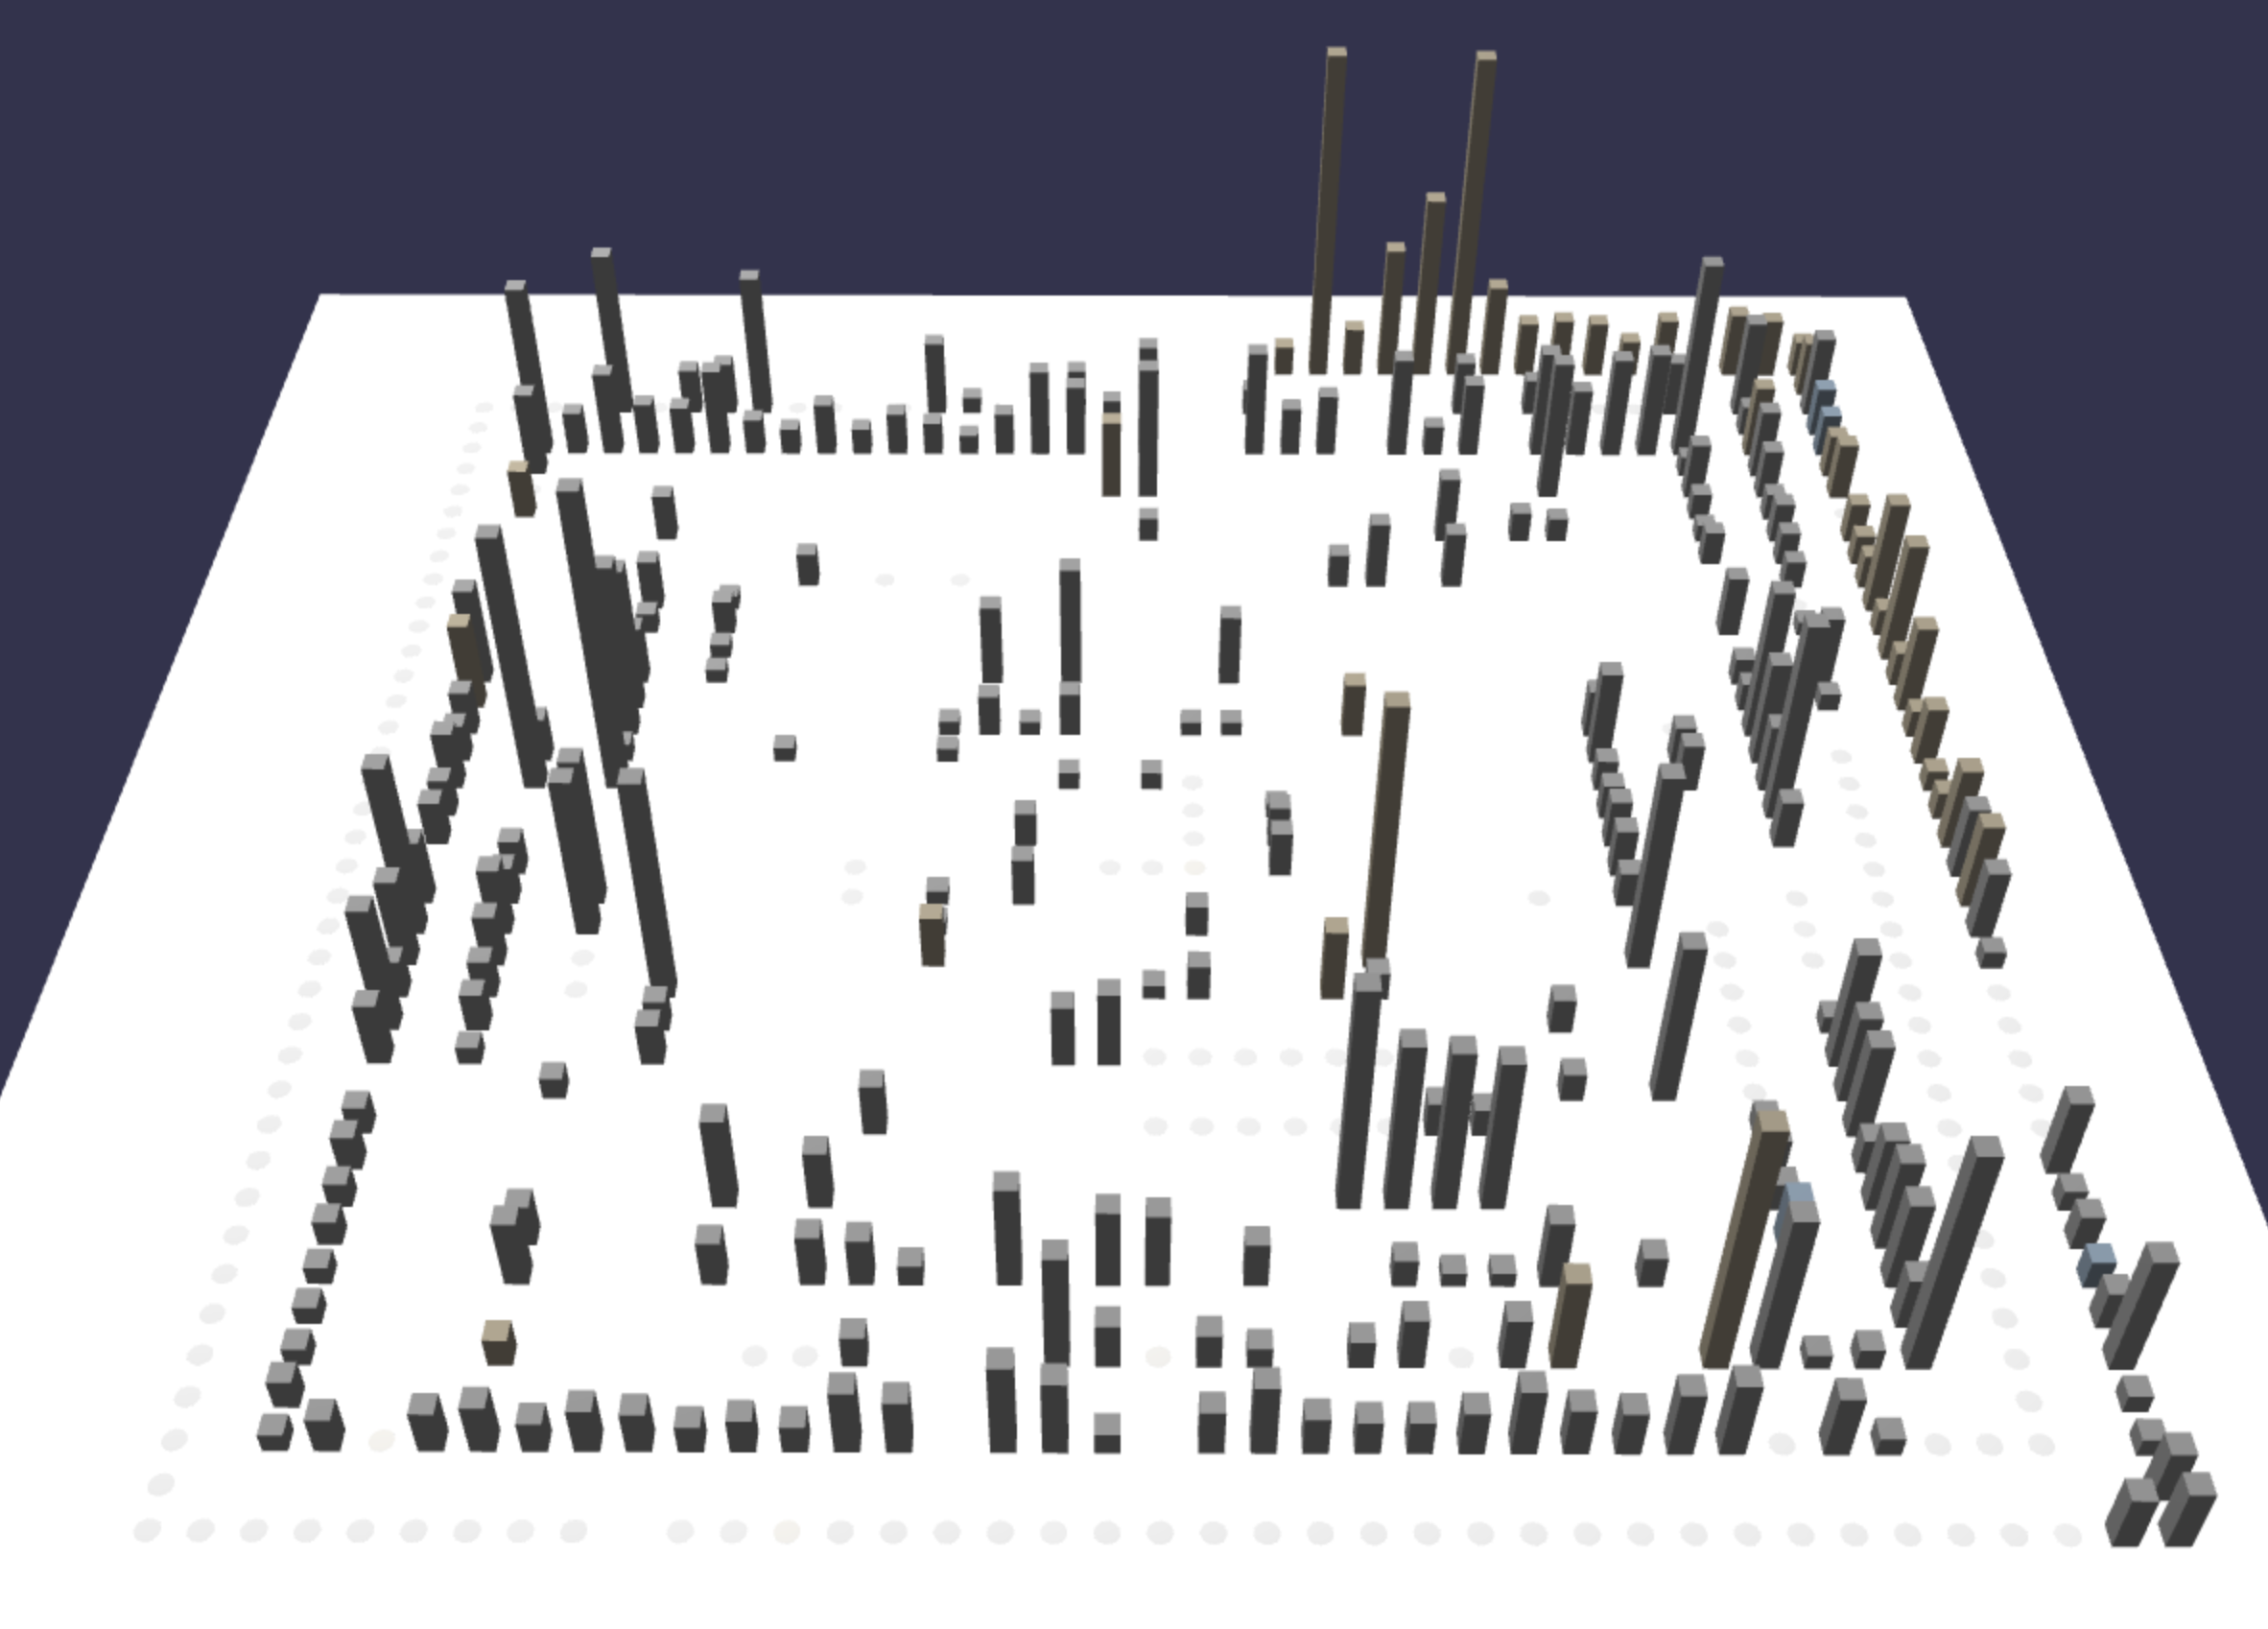
\includegraphics[width=\linewidth]{JetUML_V3S8.png}
        \caption{Year 8 (last)} 
        \label{fig:JetUML_V3S8}
    \end{subfigure}
    
    \caption{Evolution of JetUML} 
    \label{fig:JetUML_V3}
\end{figure}

% -------------------------------------------
% argouml
% FileHistories: 11129 
% ProjectVersions: 16672 
% FileVersions: 91667 
% First Version: 
% 	 hash: 6ef818a48b453627fd282971f3f9a28e28f54390 
% 	 date: Mon Jan 26 23:19:17 CET 1998 
% Last Version: 
% 	 hash: 3ddc7f94d83c4e2f439ca6fc0fe787616a1900a9 
% 	 date: Sat May 29 23:18:44 CEST 2021 
% Diff: {DAYS=128, HOURS=22, MINUTES=59, SECONDS=27, MILLISECONDS=0, MICROSECONDS=0, NANOSECONDS=0, YEARS=23}
% -------------------------------------------
\clearpage
\section{ArgoUML}
This section analyzes ArgoUML, a leading open source UML modeling tool that supports all standard UML diagrams. 
It is hosted on GitHub at the following address \url{https://github.com/argouml-tigris-org/argouml}. 
This repository was born in January 1998, converted from CVS to Subversion in 2006, and finally moved to git in 2019.
Therefore, it has more than 23 years of history. 
Our analysis considered 16'672 commits, 11'129 FileHistories, and more than 90K FileVersions. 

%\subsection{View 4}
\label{subsec:view4}
\textbf{Goal of this visualization}
This visualization aims to see how the repository evolved through these 23 years. Therefore we decided to adopt a commit grouping strategy based on a time window of 1 year and an aging strategy of one month with a total of 12 steps. Hence, grey entities represent files that have not been updated for more than 12 months. 

\bigbreak
View specification adopted: 
\begin{itemize}
    \item \texttt{versionGroupingStrategy}: timestamp.
    \item \texttt{versionGroupingChunkSize}: 31'556'926 (1 year). 
    \item \texttt{colorPalette}: default.
    \item \texttt{agingGroupingStrategy}: timestamp.
    \item \texttt{agingStepSize}: 2'629'743 (1 month).
    \item \texttt{agingSteps}: 12 steps.
    \item \texttt{mapperMetricName}: SIZE. 
    \item \texttt{fileTypeShape}: all BOX. 
    \item \texttt{fileTypeOpacity}: all 1. 
\end{itemize}

\textbf{Results}
Here we present only the relevant aspects of the ArgoUML evolution that we have found. However, in \autoref{app:ArgoUML_Evolution} the full evolution is depicted. \autoref{fig:JetUML_V3} shows the hot spots during the system's evolution. \autoref{fig:ArgoUML_V3_S1} shows the system's state after the first year of activity. As we can notice, almost all the entities have a color different than gray. This means that they were updated between April 1998 and January 1999 because they should be darker or gray otherwise. The size of the system was constantly increasing when in 2003, as \autoref{fig:ArgoUML_V3_S2} shows, the system's core was entirely rewritten. Three years later it had another important refactoring; in fact, as we can see in figure \autoref{fig:ArgoUML_V3_S3} there are some empty rings around the center and a bigger size than the year before. Our interpretation of this event is that an entire set of consequently added files was removed and maybe later added. It is important to underline that these files were deleted, not moved, or renamed because otherwise, SYN would treat them as the same logical entity. The same event happened four years later, when the system was ten years old. 2010 was the last truly active year for the repository as depicted in \autoref{fig:ArgoUML_V3_S5}; almost all the repository files were modified and we can notice more taller entities, meaning that the overall size of the files increased. The system did not grow up anymore after that year. Sometimes some files were updated until 2014 when they became almost dead. During 2019 they made a commit that removed lots of files \footnote{\url{https://github.com/argouml-tigris-org/argouml/commit/62d5393eeaf08b749b17107faef255a22da55ce5}}. As a result, in January 2020, as represented in \autoref{fig:ArgoUML_V3_S6}, the visualization has more blank spots, and since there was no activity, with the exceptions of few files, almost all the entities are painted with gray. In June 2022, the system is pretty identical to its version in 2020. 

\bigbreak
\textbf{Conclusion}
Thanks to this analysis, we have understood the composition of JetUML and at which speed it grew. Thanks to the spiral layout, where entities are added based on their timestamp, we can understand that many older files were removed in the final version. They had to be rewritten elsewhere because the system would have fewer features than before. Moreover, thanks to the aging strategy, we have understood that there was much dead time during the development lifecycle of the repository. Nonetheless, some of them are not shown in \autoref{fig:JetUML_V3}, they can be found in \autoref{app:ArgoUML_Evolution}. The system became almost dead in 2014; since that year, most of the files were never updated. 



\begin{figure}[ht]
    \begin{subfigure}{0.48\textwidth}
        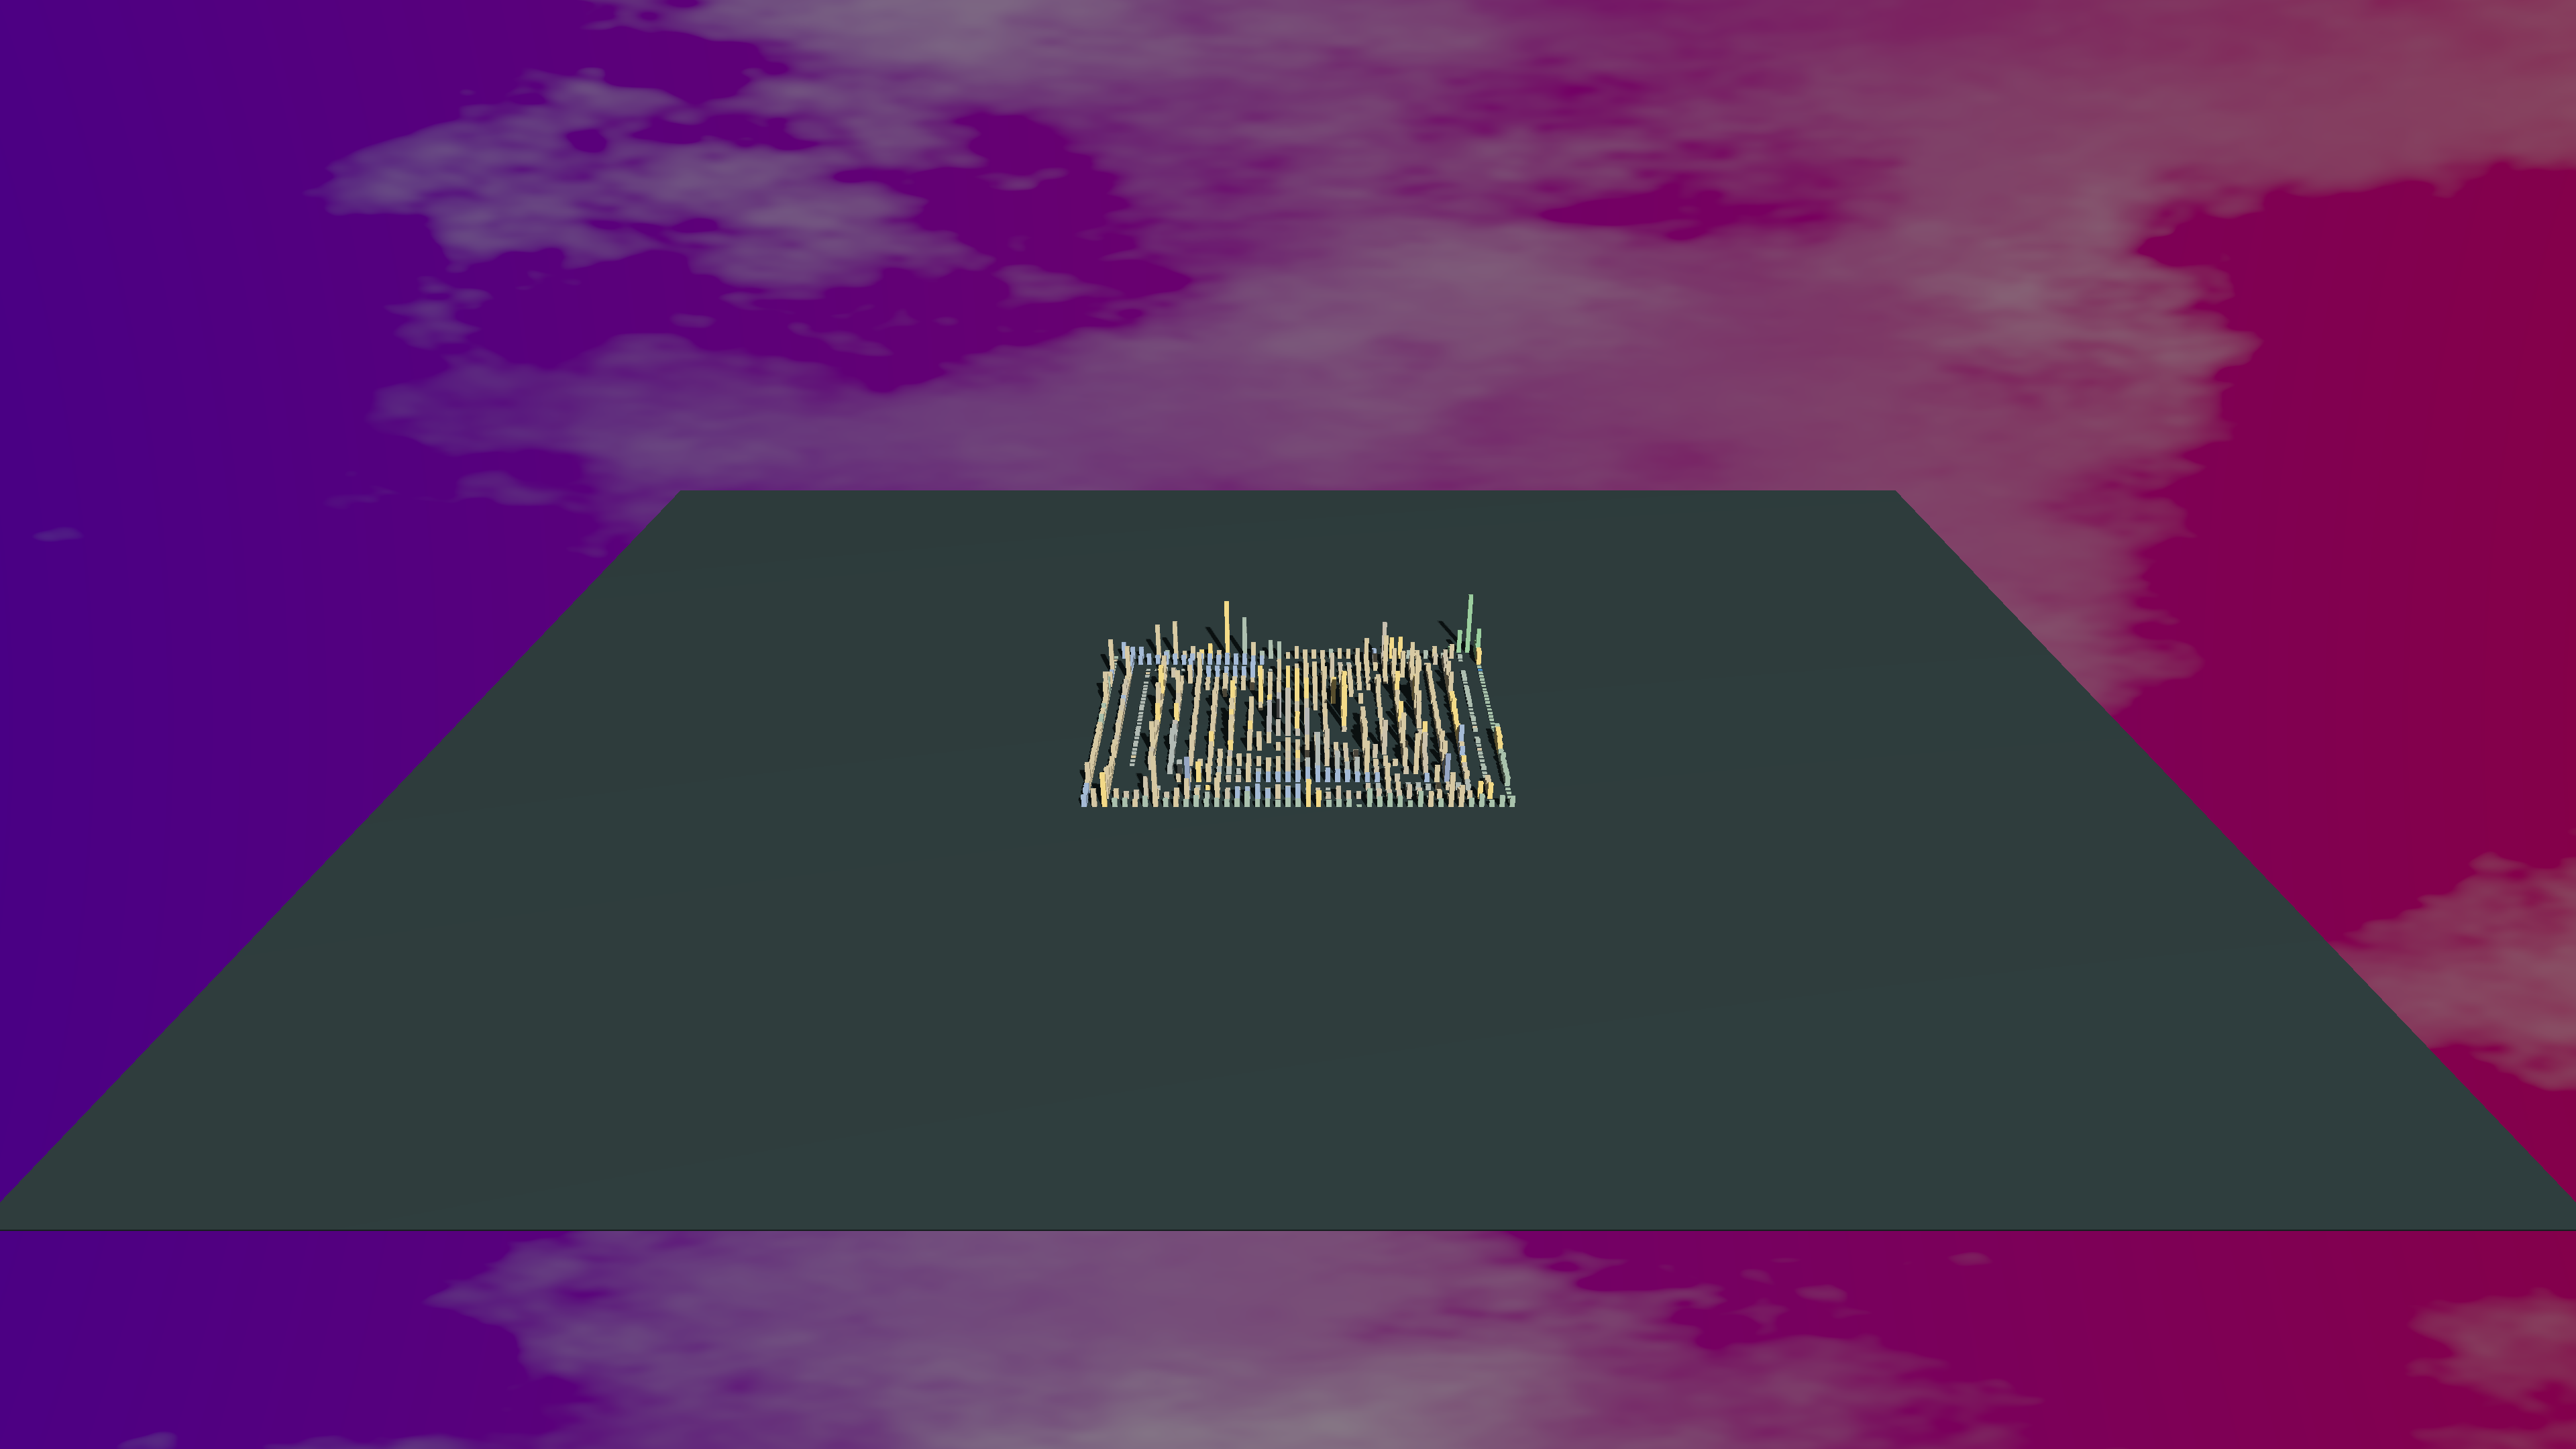
\includegraphics[width=\linewidth]{ArgoUML/Animation001.png}
        \caption{ArgoUML in Jenuary 1999 (1 year)} 
        \label{fig:ArgoUML_V3_S1}
    \end{subfigure}\hspace*{\fill}
    \begin{subfigure}{0.48\textwidth}
        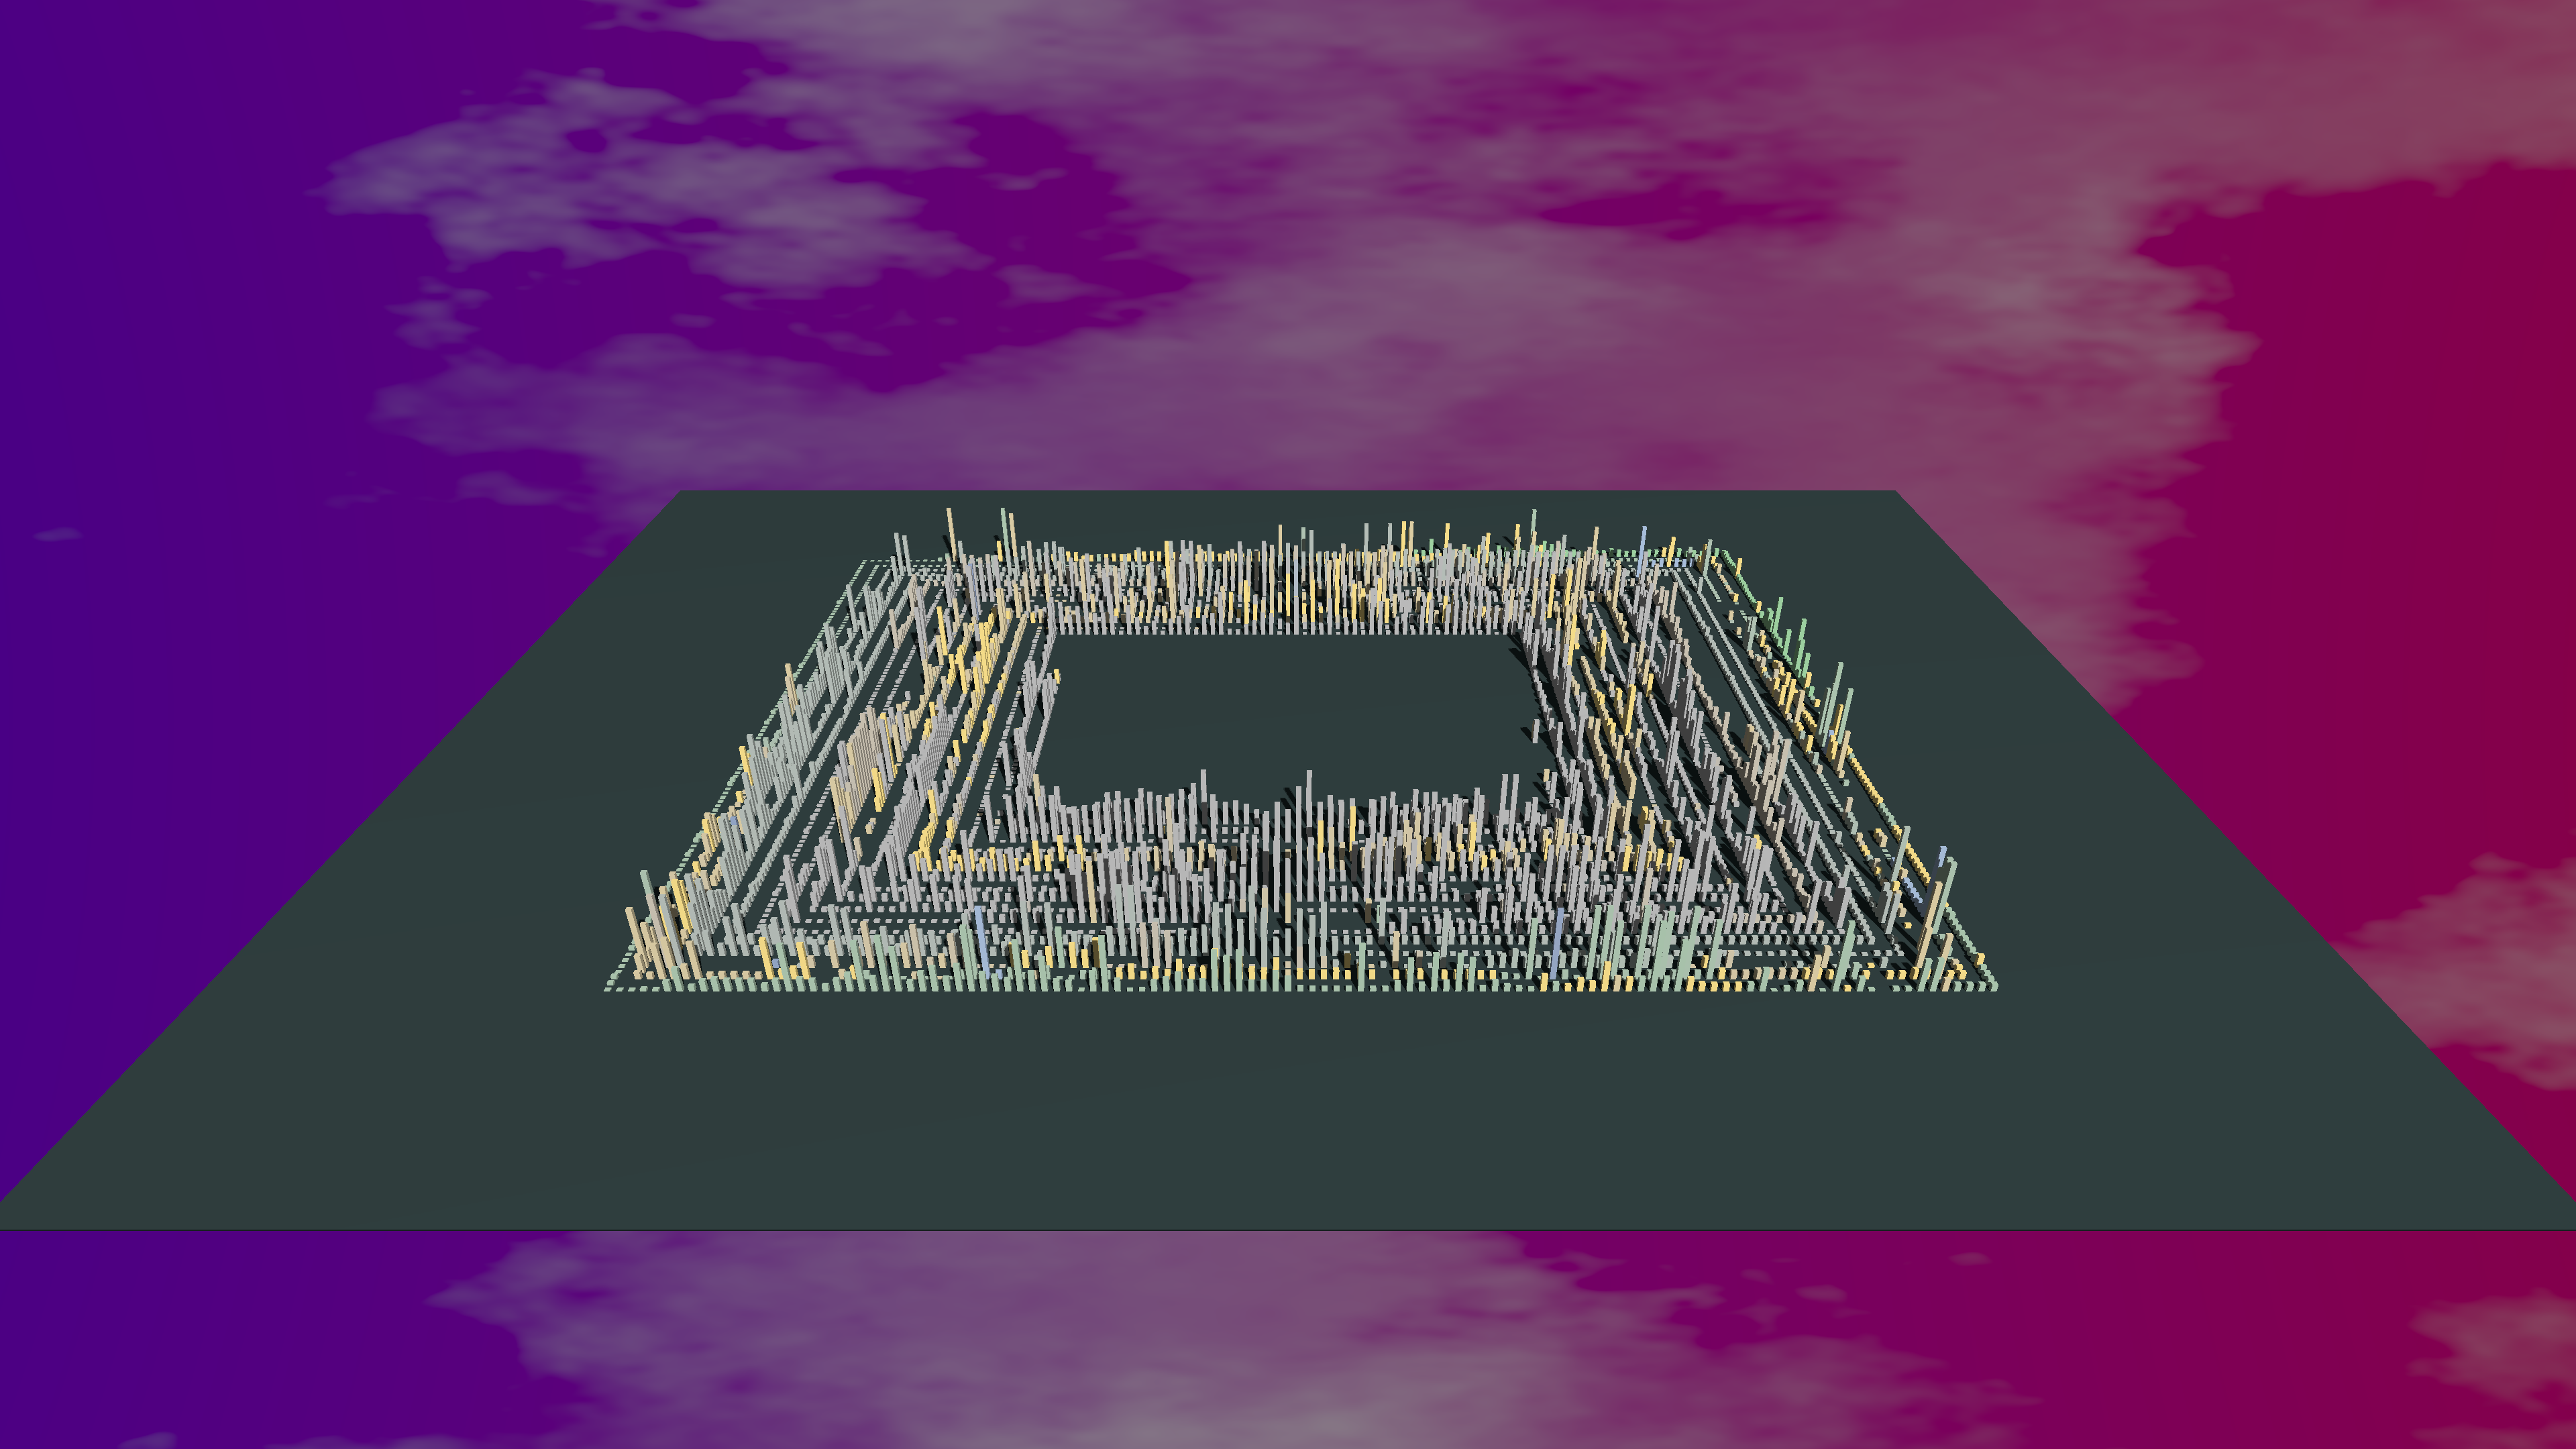
\includegraphics[width=\linewidth]{ArgoUML/Animation005.png}
        \caption{ArgoUML in Jenuary 2003 (5 years)} 
        \label{fig:ArgoUML_V3_S2}
    \end{subfigure}
    \medskip
    \begin{subfigure}{0.48\textwidth}
        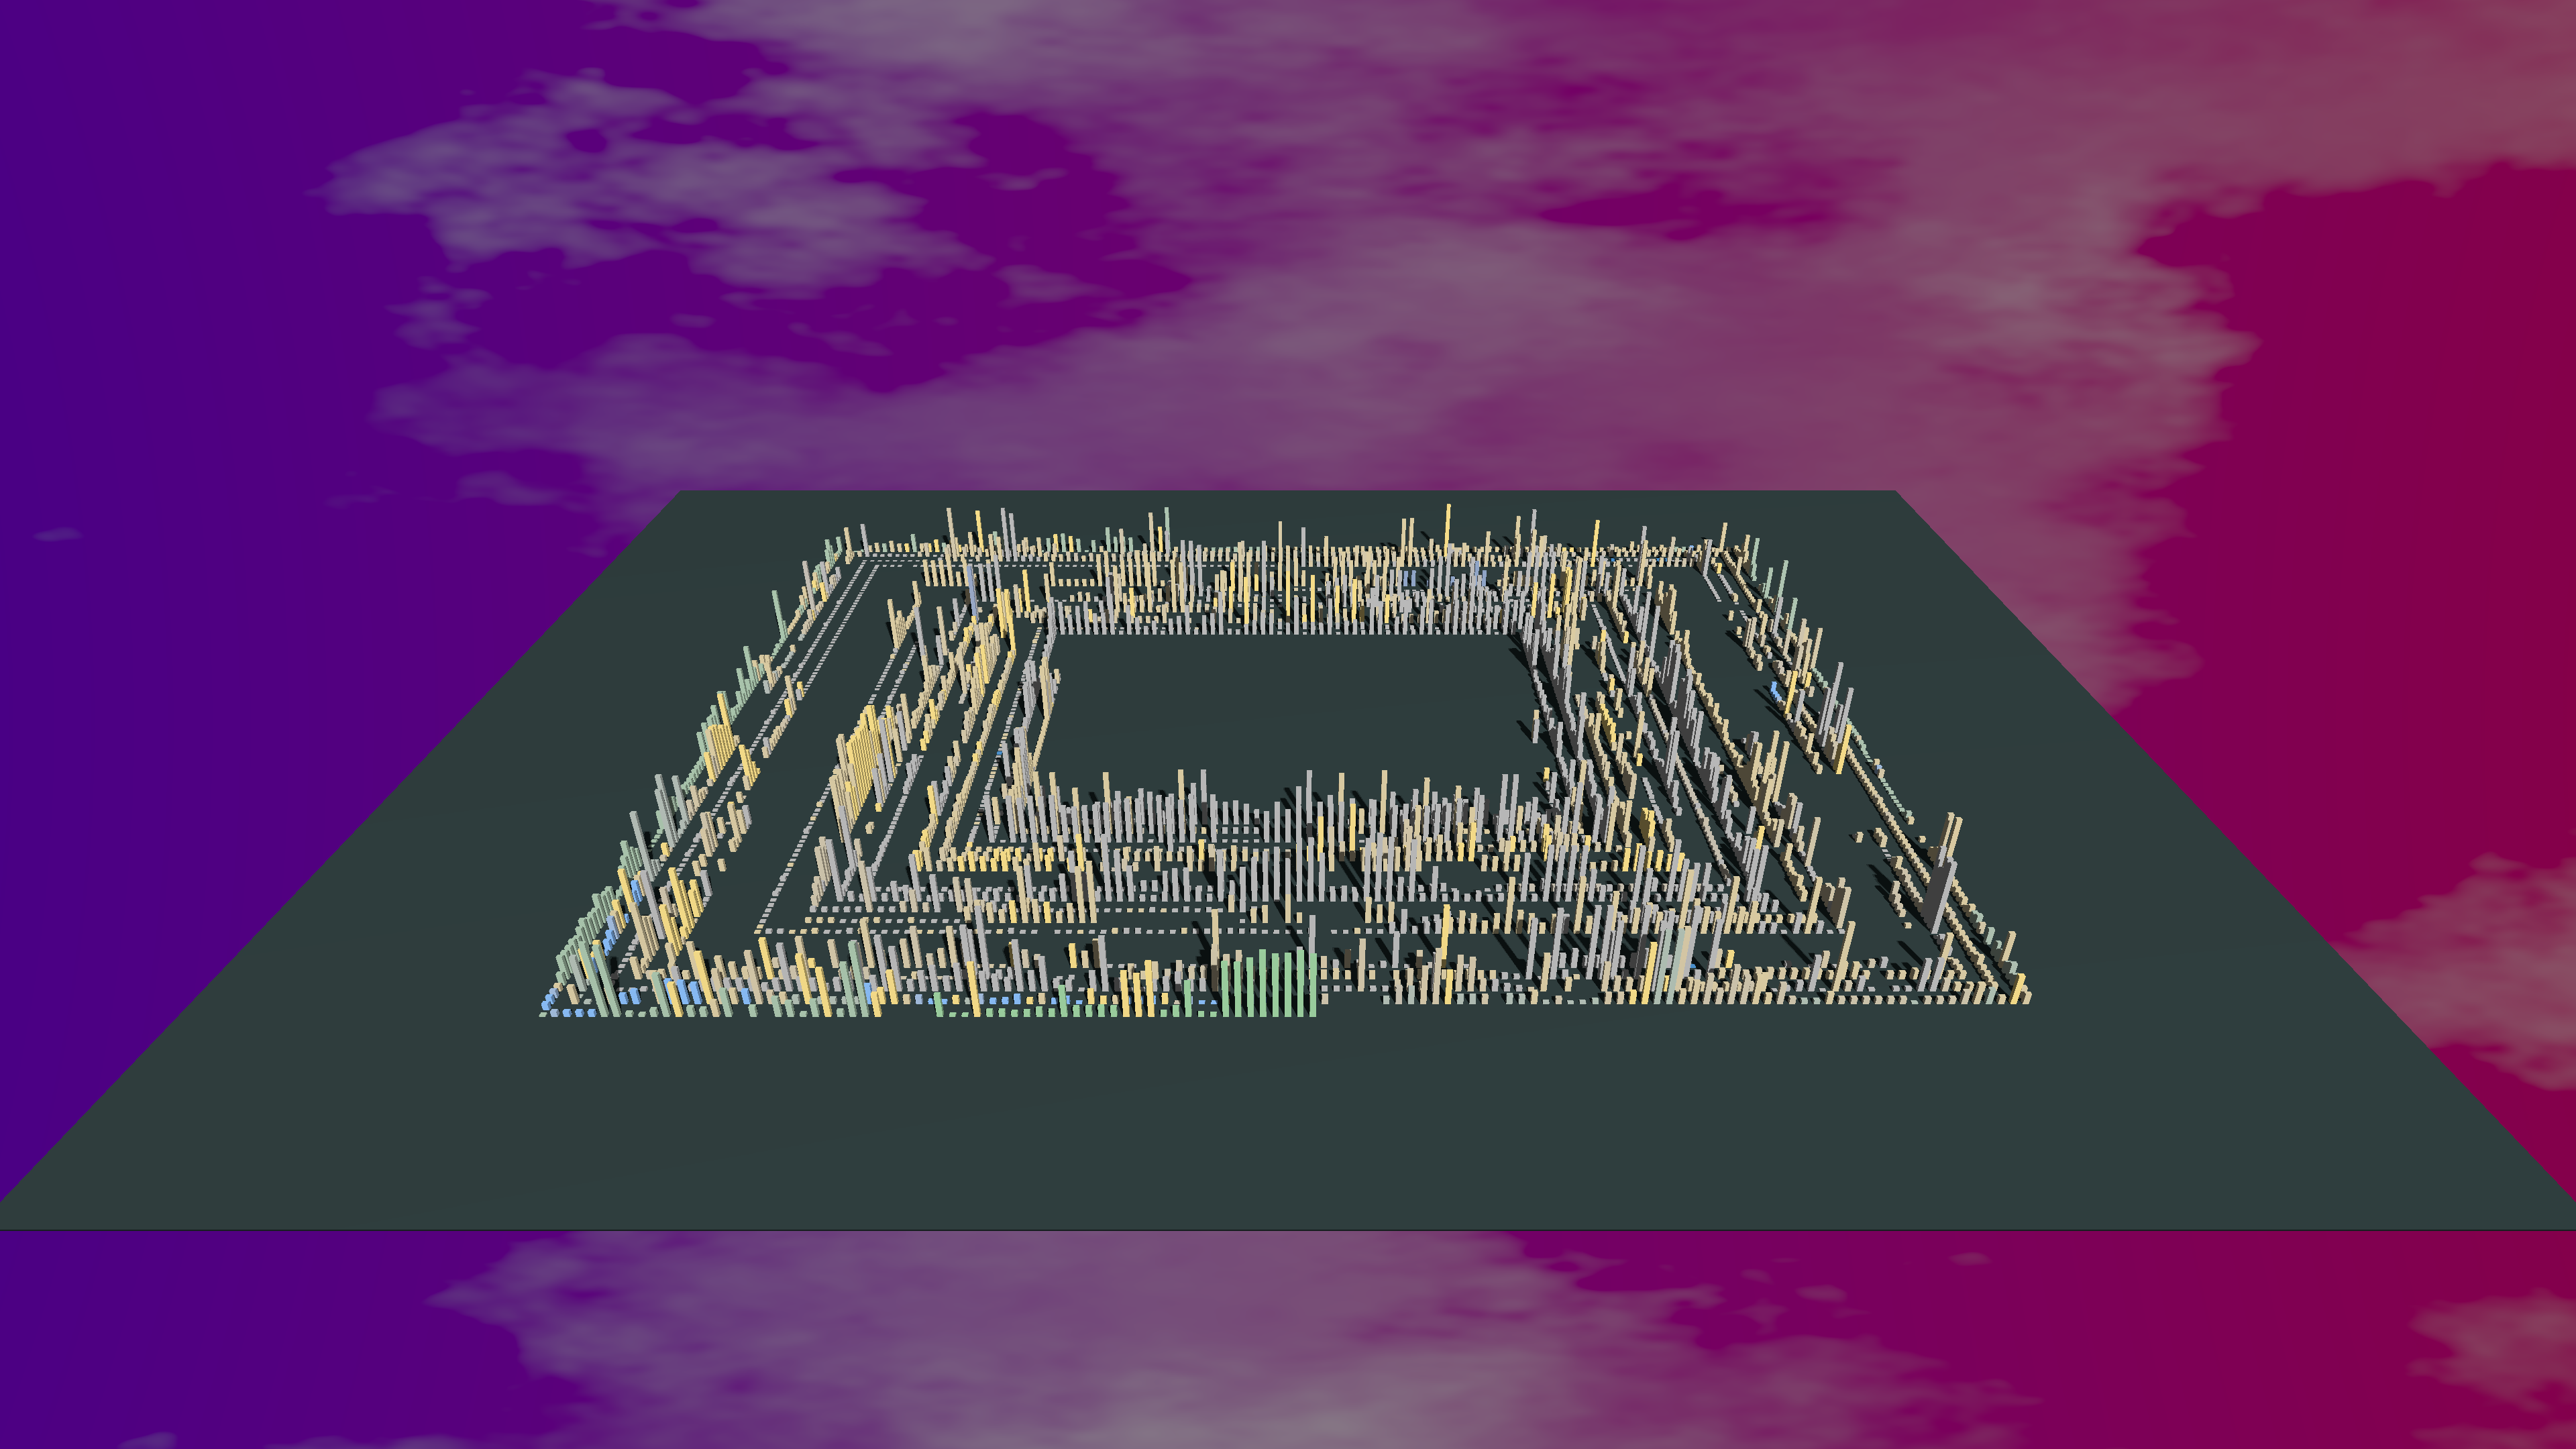
\includegraphics[width=\linewidth]{ArgoUML/Animation006.png}
        \caption{ArgoUML in Jenuary 2006 (6 years)} 
        \label{fig:ArgoUML_V3_S3}
    \end{subfigure}\hspace*{\fill}
    \begin{subfigure}{0.48\textwidth}
        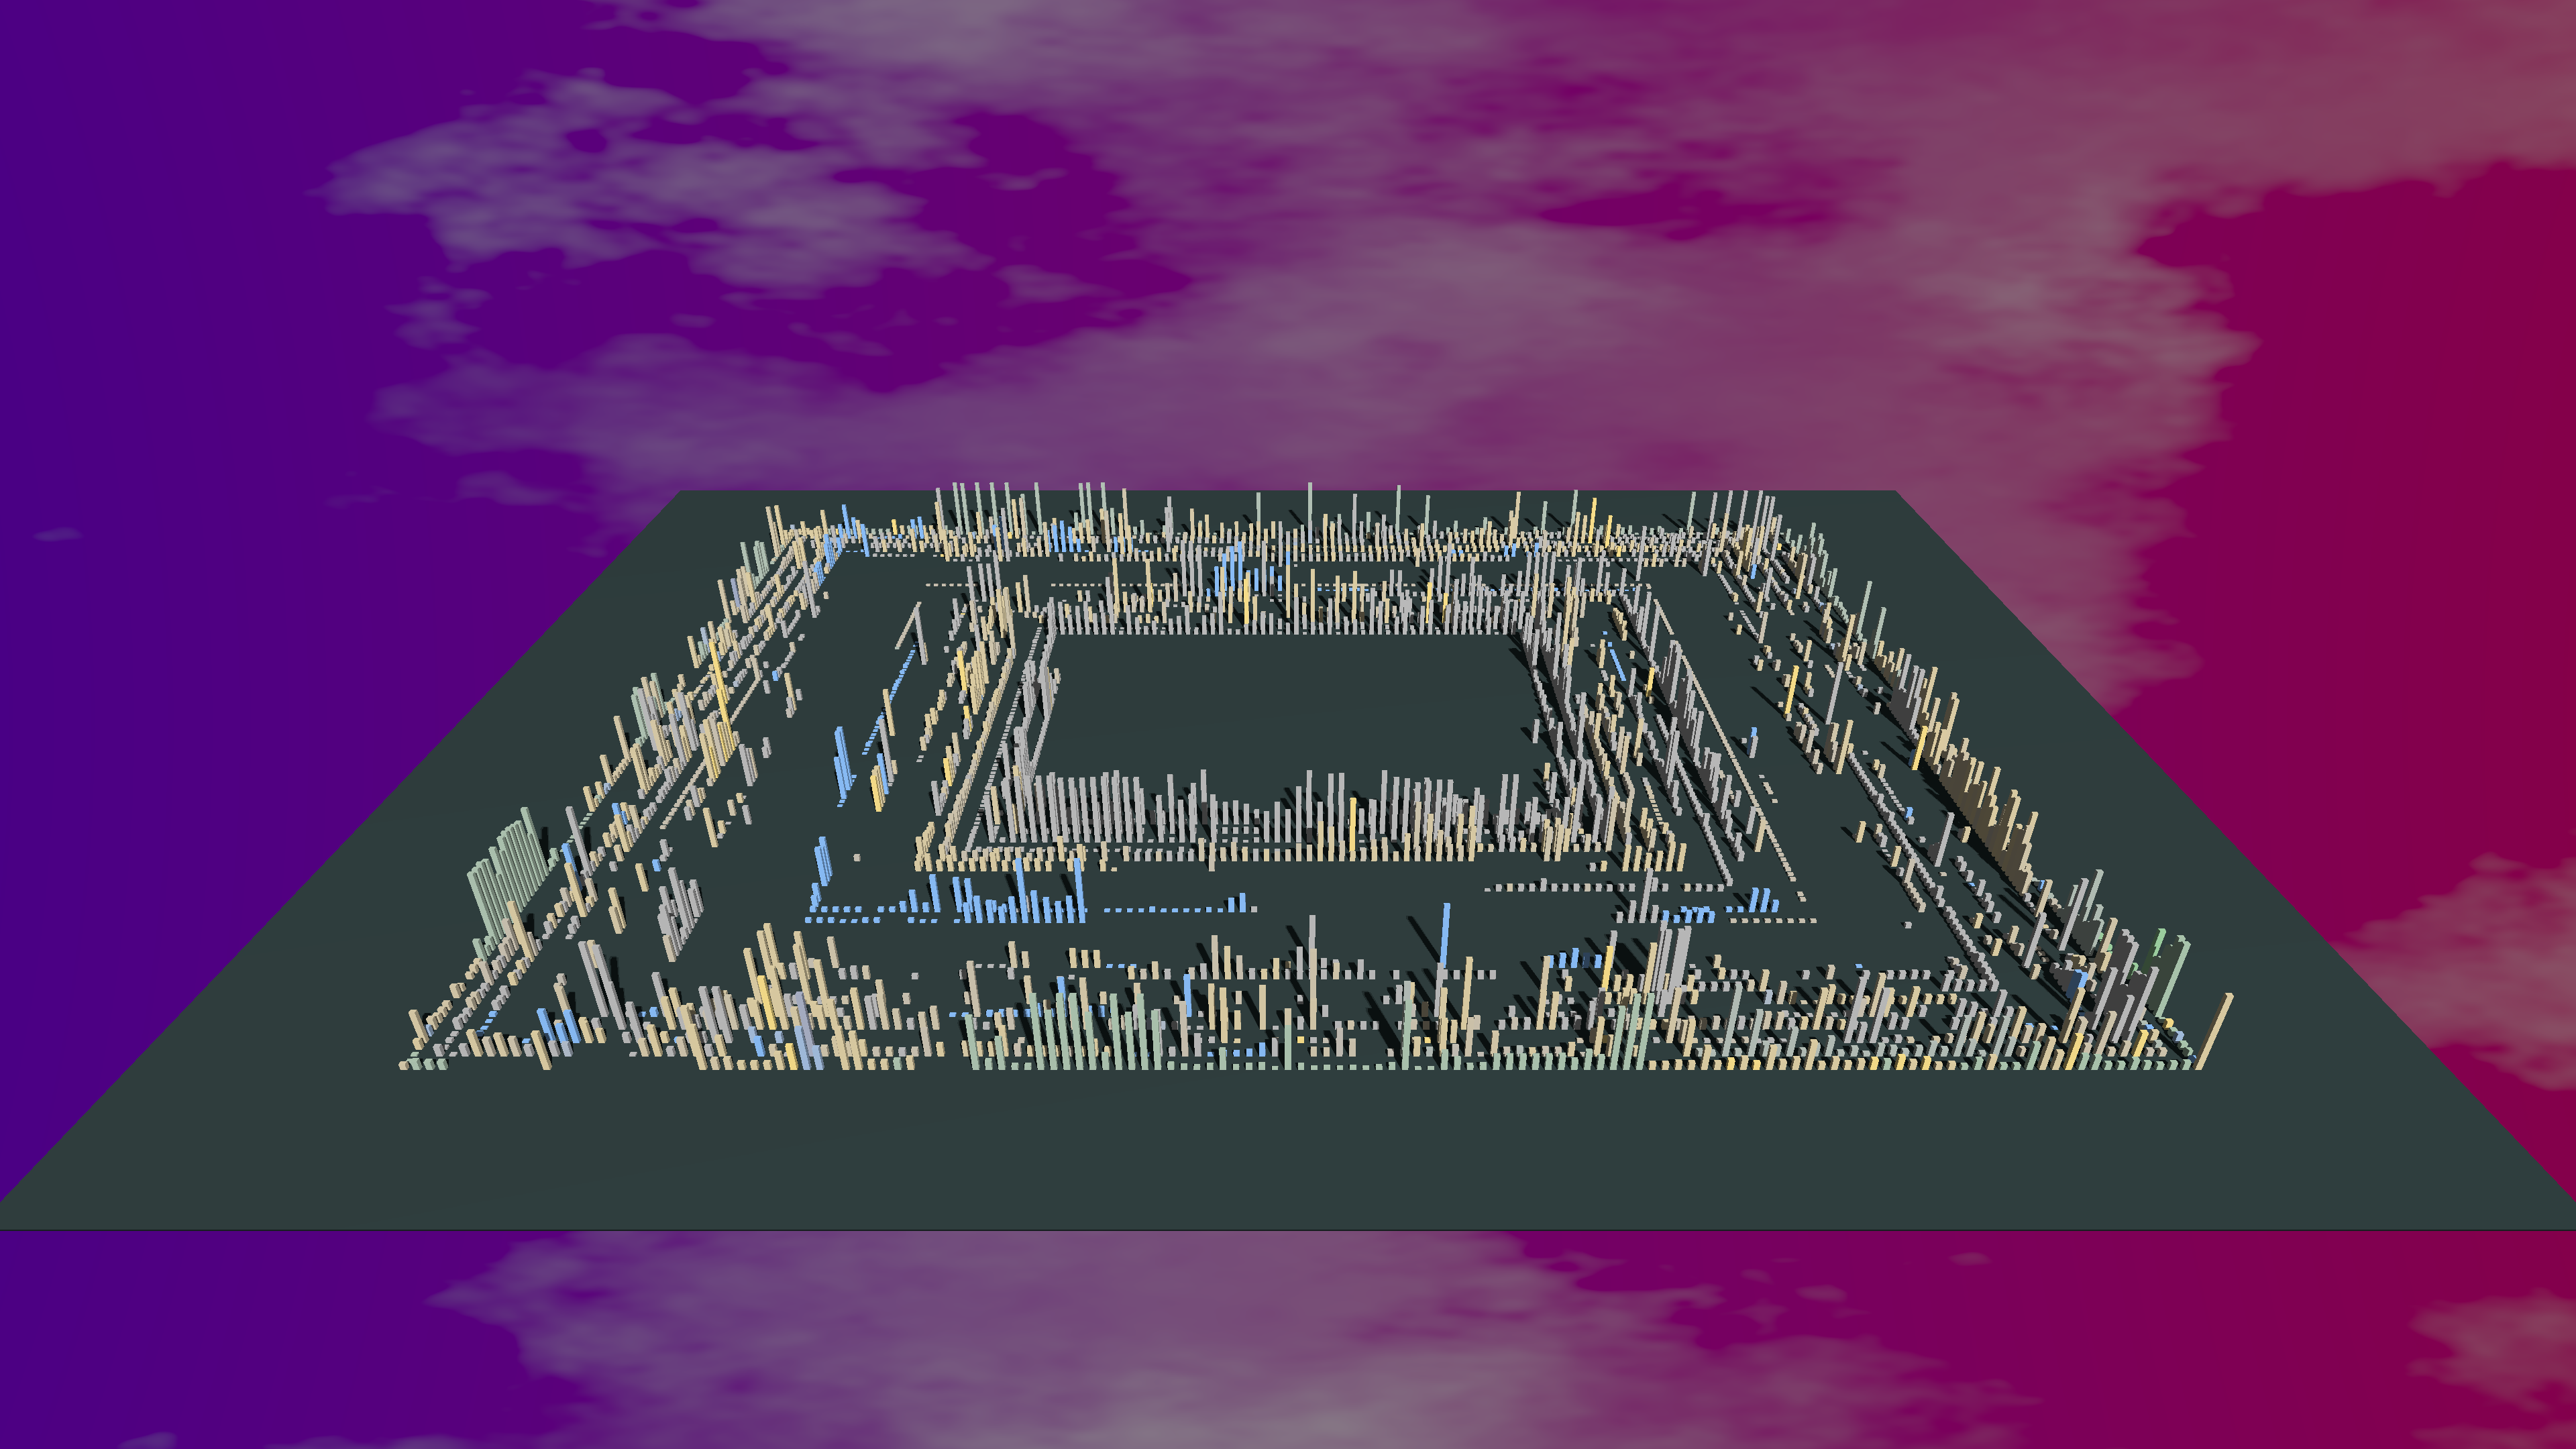
\includegraphics[width=\linewidth]{ArgoUML/Animation010.png}
        \caption{ArgoUML in Jenuary 2008 (10 years)} 
        \label{fig:ArgoUML_V3_S4}
    \end{subfigure}
    \medskip
    \begin{subfigure}{0.48\textwidth}
        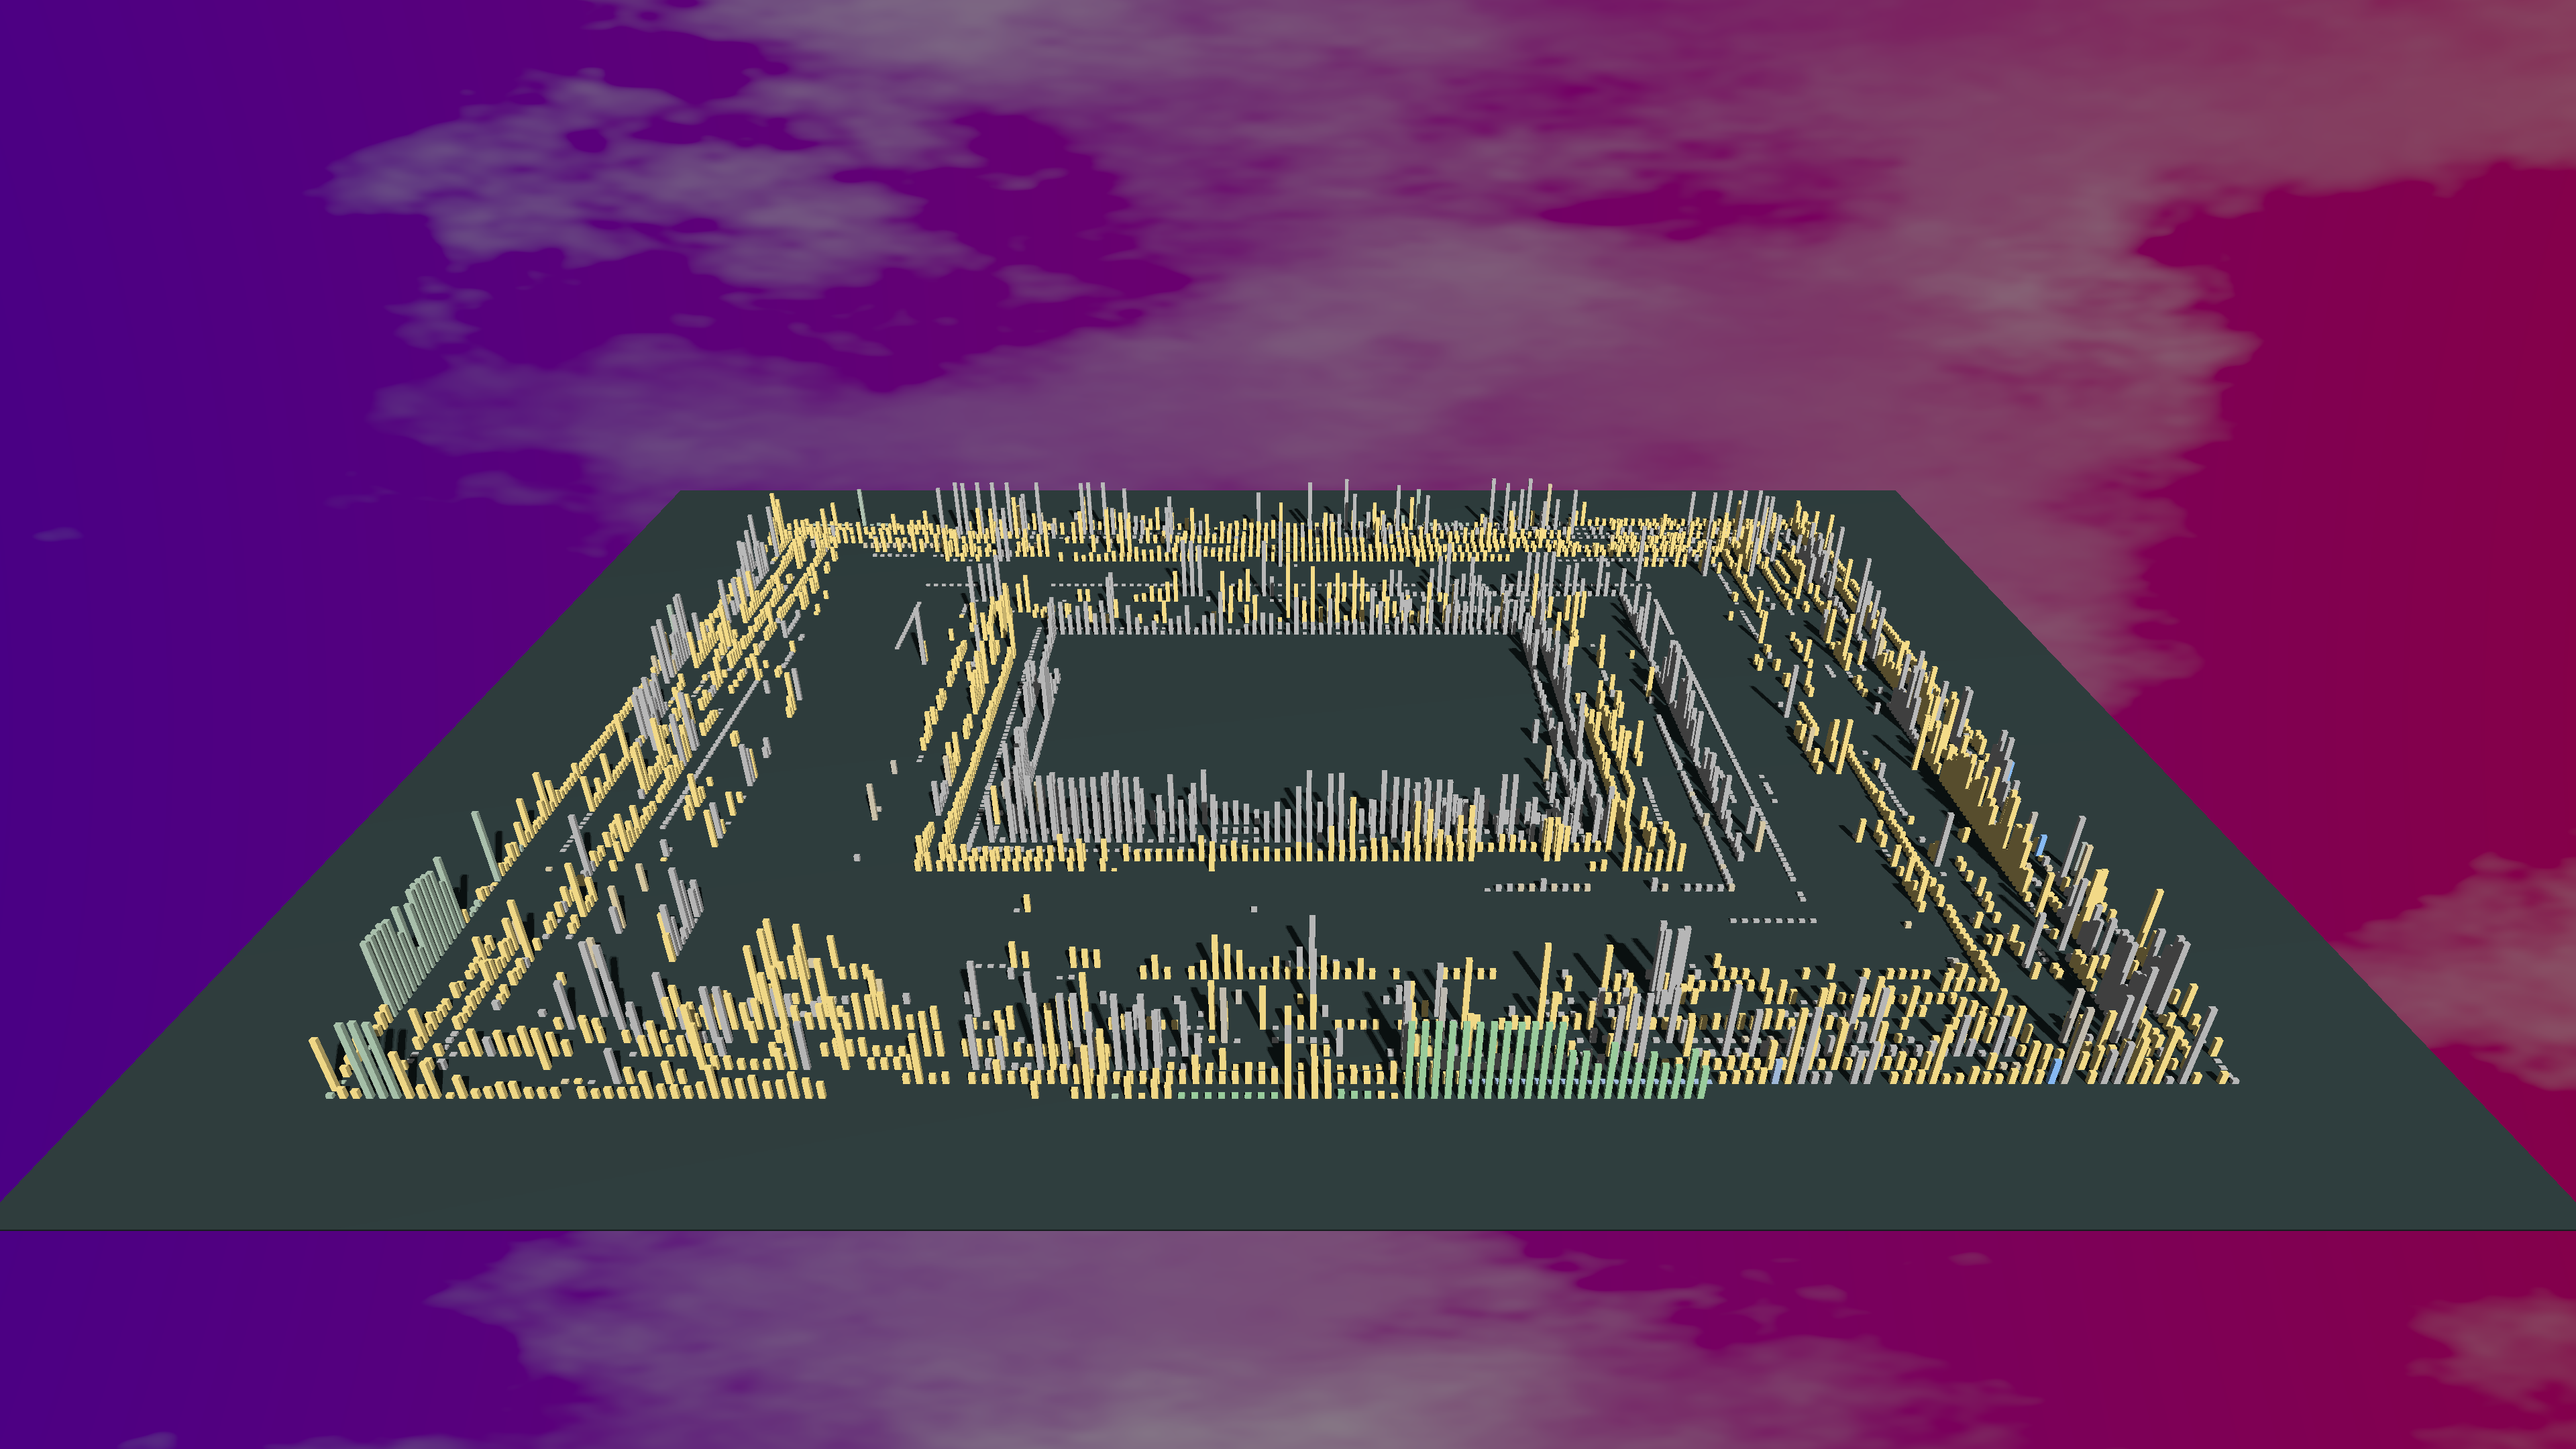
\includegraphics[width=\linewidth]{ArgoUML/Animation012.png}
        \caption{ArgoUML in Jenuary 2010 (12 years)} 
        \label{fig:ArgoUML_V3_S5}
    \end{subfigure}\hspace*{\fill}
    \begin{subfigure}{0.48\textwidth}
        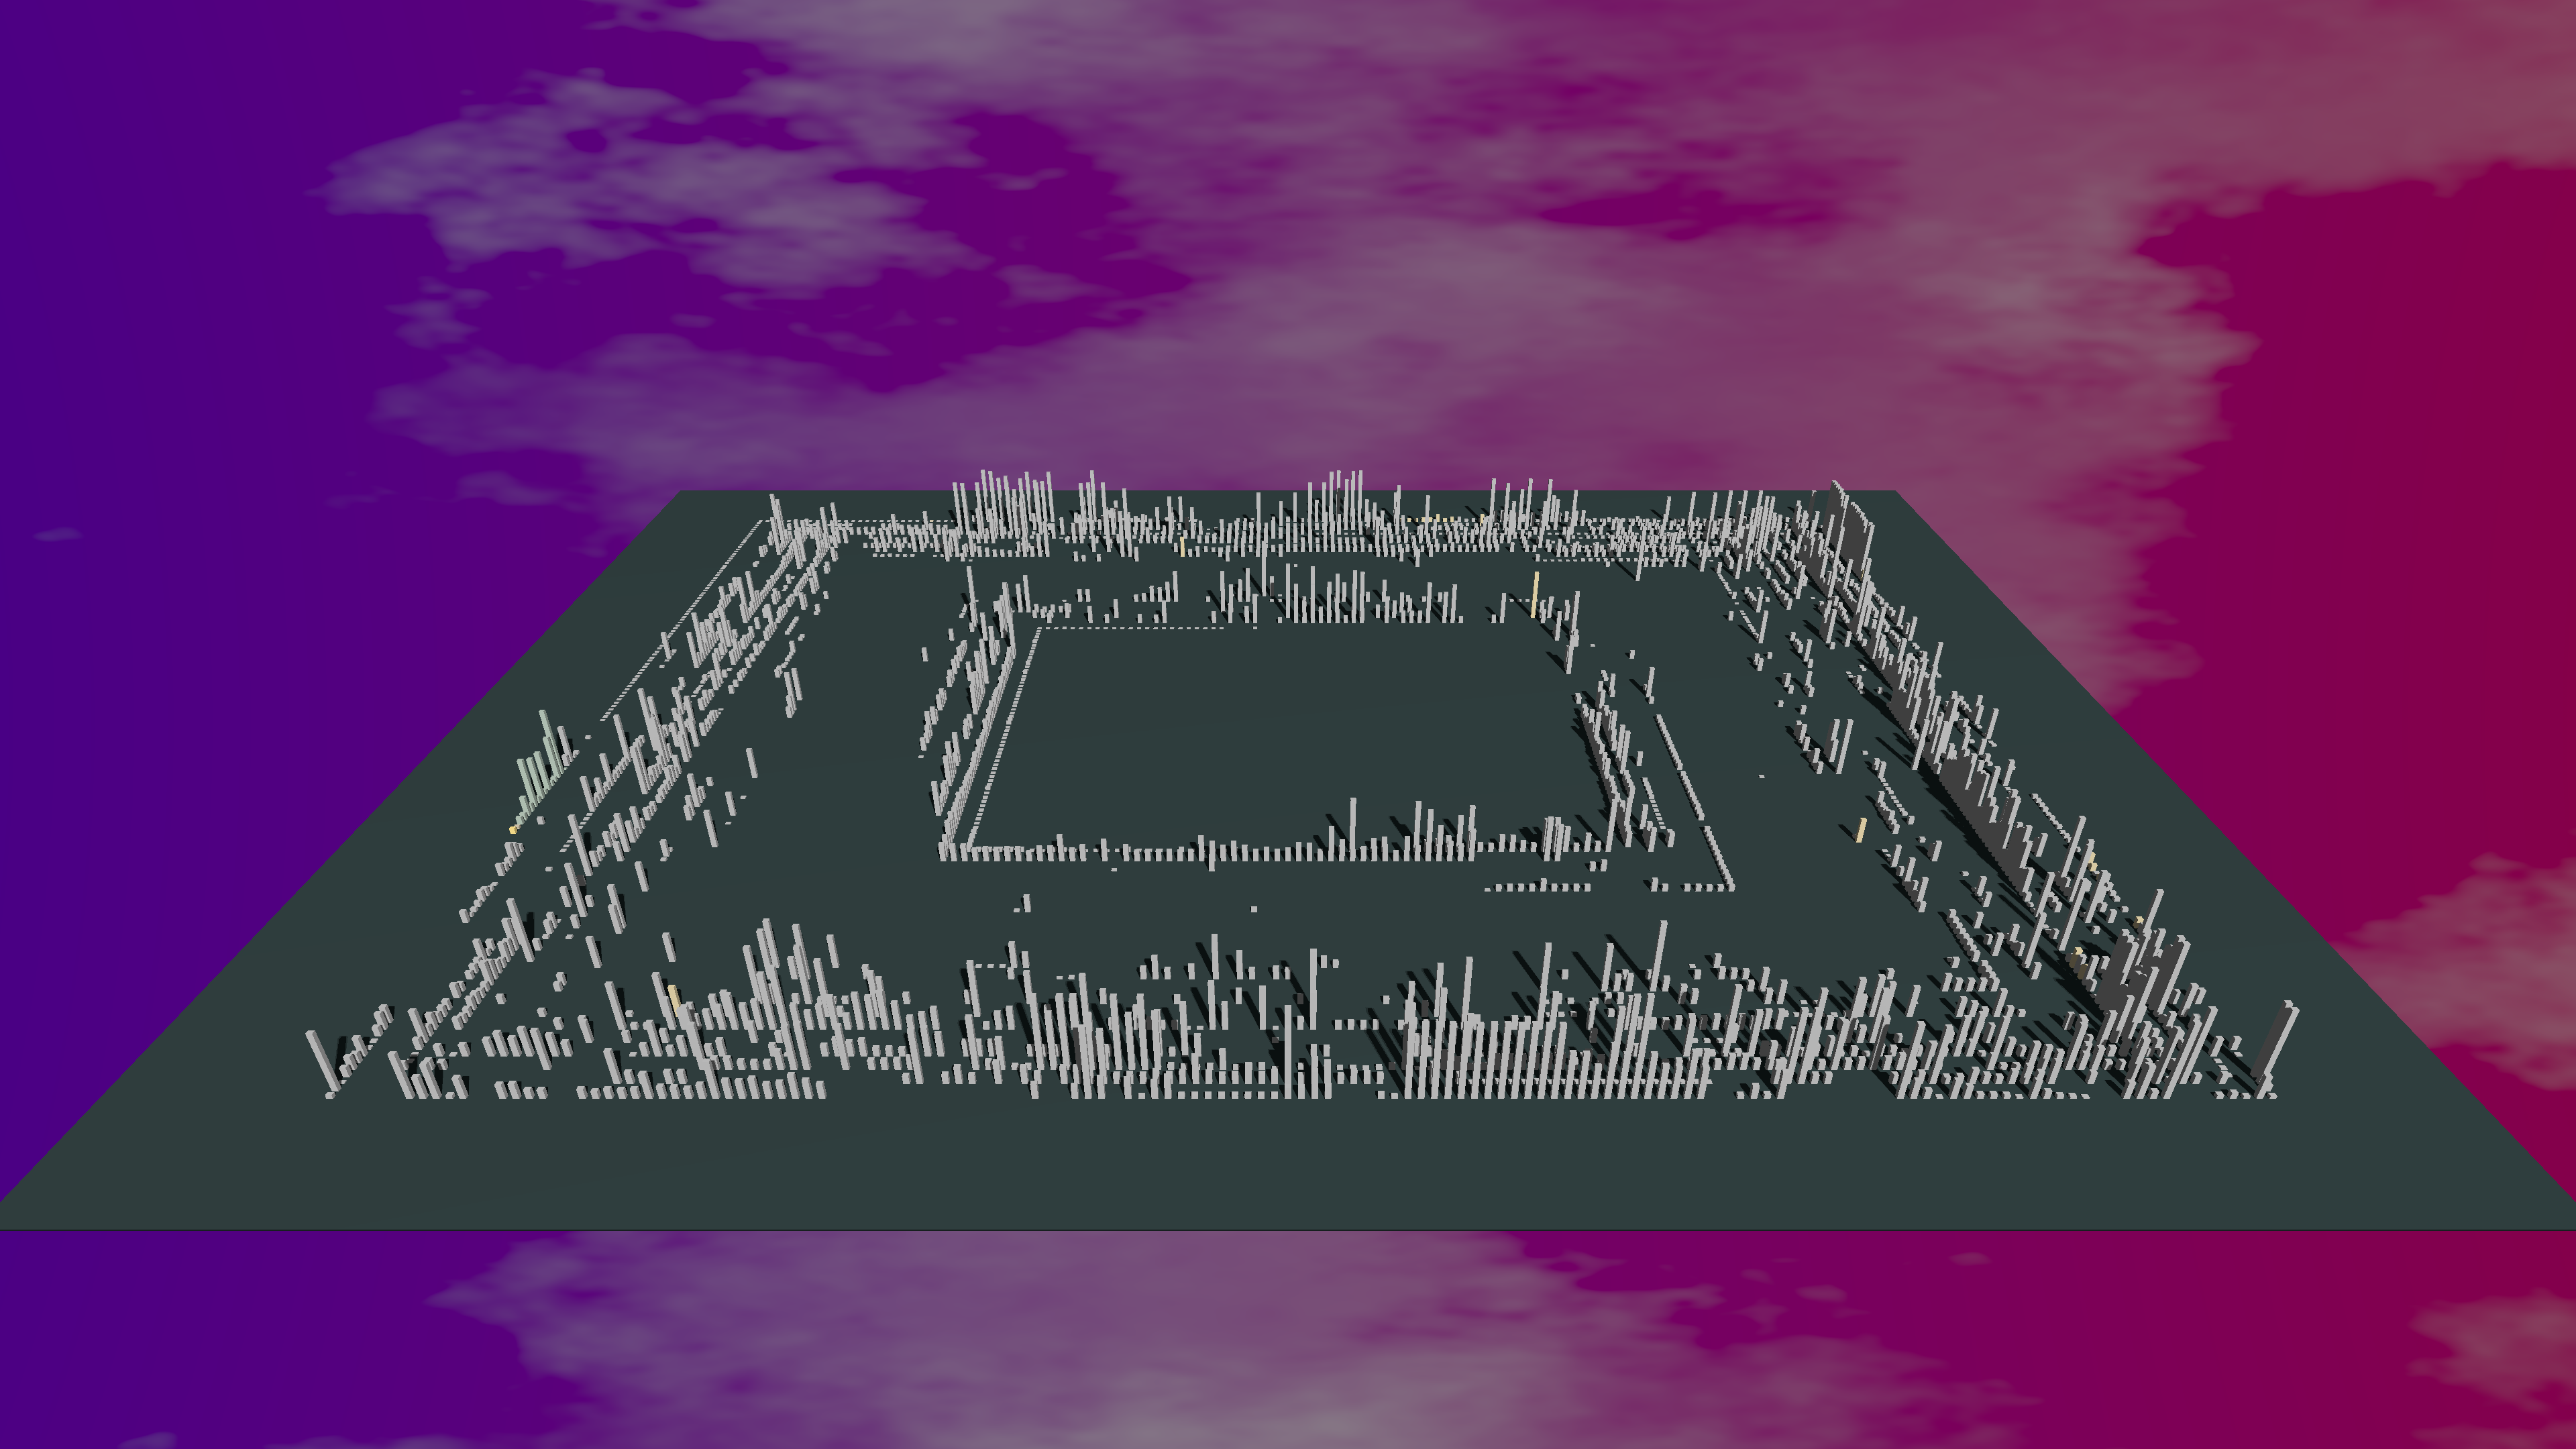
\includegraphics[width=\linewidth]{ArgoUML/Animation022.png}
        \caption{ArgoUML in Jenuary 2020 (22 years)} 
        \label{fig:ArgoUML_V3_S6}
    \end{subfigure}
    
    \caption{Hot spots during the evolution of ArgoUML} 
    \label{fig:JetUML_V3}
\end{figure}
\clearpage
% -------------------------------------------
% elastic
% FileHistories: 41043 
% ProjectVersions: 34842 
% FileVersions: 326543 
% First Version: 
% 	 hash: 222b36344f0939f12cf54358e7047239cd398463 
% 	 date: Fri Jun 28 09:22:10 CEST 2013 
% Last Version: 
% 	 hash: 2cdffdce2ab35416bd5b1b7ea889cd0dede5b6c8 
% 	 date: Thu Apr 14 14:36:03 CEST 2022 
% Diff: {DAYS=292, HOURS=5, MINUTES=13, SECONDS=53, MILLISECONDS=0, MICROSECONDS=0, NANOSECONDS=0, YEARS=8}
% -------------------------------------------

\section{Elasticsearch}
This section analyzes Elasticsearch, a distributed, RESTful JSON-based search, and analytics engine. 
The project is open-source and hosted on GitHub at \url{https://github.com/elastic/elasticsearch}. 
The first commit was made in June 2013, even though it was not the real first one because the project started four years before in 2009. 
Our analysis comprehends almost nine years of history, in which there are 34'843 ProjectVersions, 41'043 FileHistories, and more than 300K FileVersions. 

%\subsection{View 5}
\textbf{Goal of this visualization}
This visualization aims to see how the repository evolved through its last nine years. We decided to adopt a commit grouping strategy based on a time window of 1 year and an aging strategy of one month with 12 steps. Hence, grey entities represent files that have not been updated for more than 12 months. 

\bigbreak
View specification adopted: same as the one defined for the View 4 (\autoref{subsec:view4}).

\textbf{Results}
Here we present only the relevant aspects of the ArgoUML evolution that we have found. However, in \autoref{app:Elastic_Evolution} the full evolution is depicted. \autoref{fig:Elastic_V5} shows the hot spots during the system's evolution. \autoref{fig:Elastic_V5_S1} shows the initial size of the system when the system became open source and was officially moved on GitHub. After one year of inactivity, the size of the system in June 2016 was almost triple of 2 years before. If on June 2014, it had 2'904 files; in June 2016, it had 9'537 files. However, in figure \autoref{fig:Elastic_V5_S2}, we notice that only the entities around the center of the system were touched. This means that the initial implementation of elastic remained untouched and that any of the files added in 2013 were modified. Perhaps the code was stable enough that it did not require any maintenance, and only new features were added before June 2016. After one year of stopping, in June 2018, we had another big increment of the system, as shown by \autoref{fig:Elastic_V5_S3}. Also, there it doubled its size. Interestingly, the core also remained untouched, except for very few changes. Moreover, the height of entities present in \autoref{fig:Elastic_V5_S2} became higher. This not only means that they were modified, but it might also mean that new features were added to these classes. We recorded the same growth pattern later in time until June 2022. As depicted in \autoref{fig:Elastic_V5_S4}, \autoref{fig:Elastic_V5_S5}, \autoref{fig:Elastic_V5_S6} the system incremented the number and the size of files gradually. The most important thing is that, except for the center, most of the files are painted with a bright color, meaning they are maintained. 


\bigbreak
\textbf{Conclusion} This analysis highlighted many interesting aspects of the Elasticsearch evolution. Among all, the most important might be that the core of the system, once developed, was never touched (except for very few entities). As we can notice from the figures shown in  \autoref{fig:Elastic_V5}, it is always depicted in gray, even if files around it are modified even in the last year of evolution. 

\begin{figure}[ht]
    \begin{subfigure}{0.48\textwidth}
        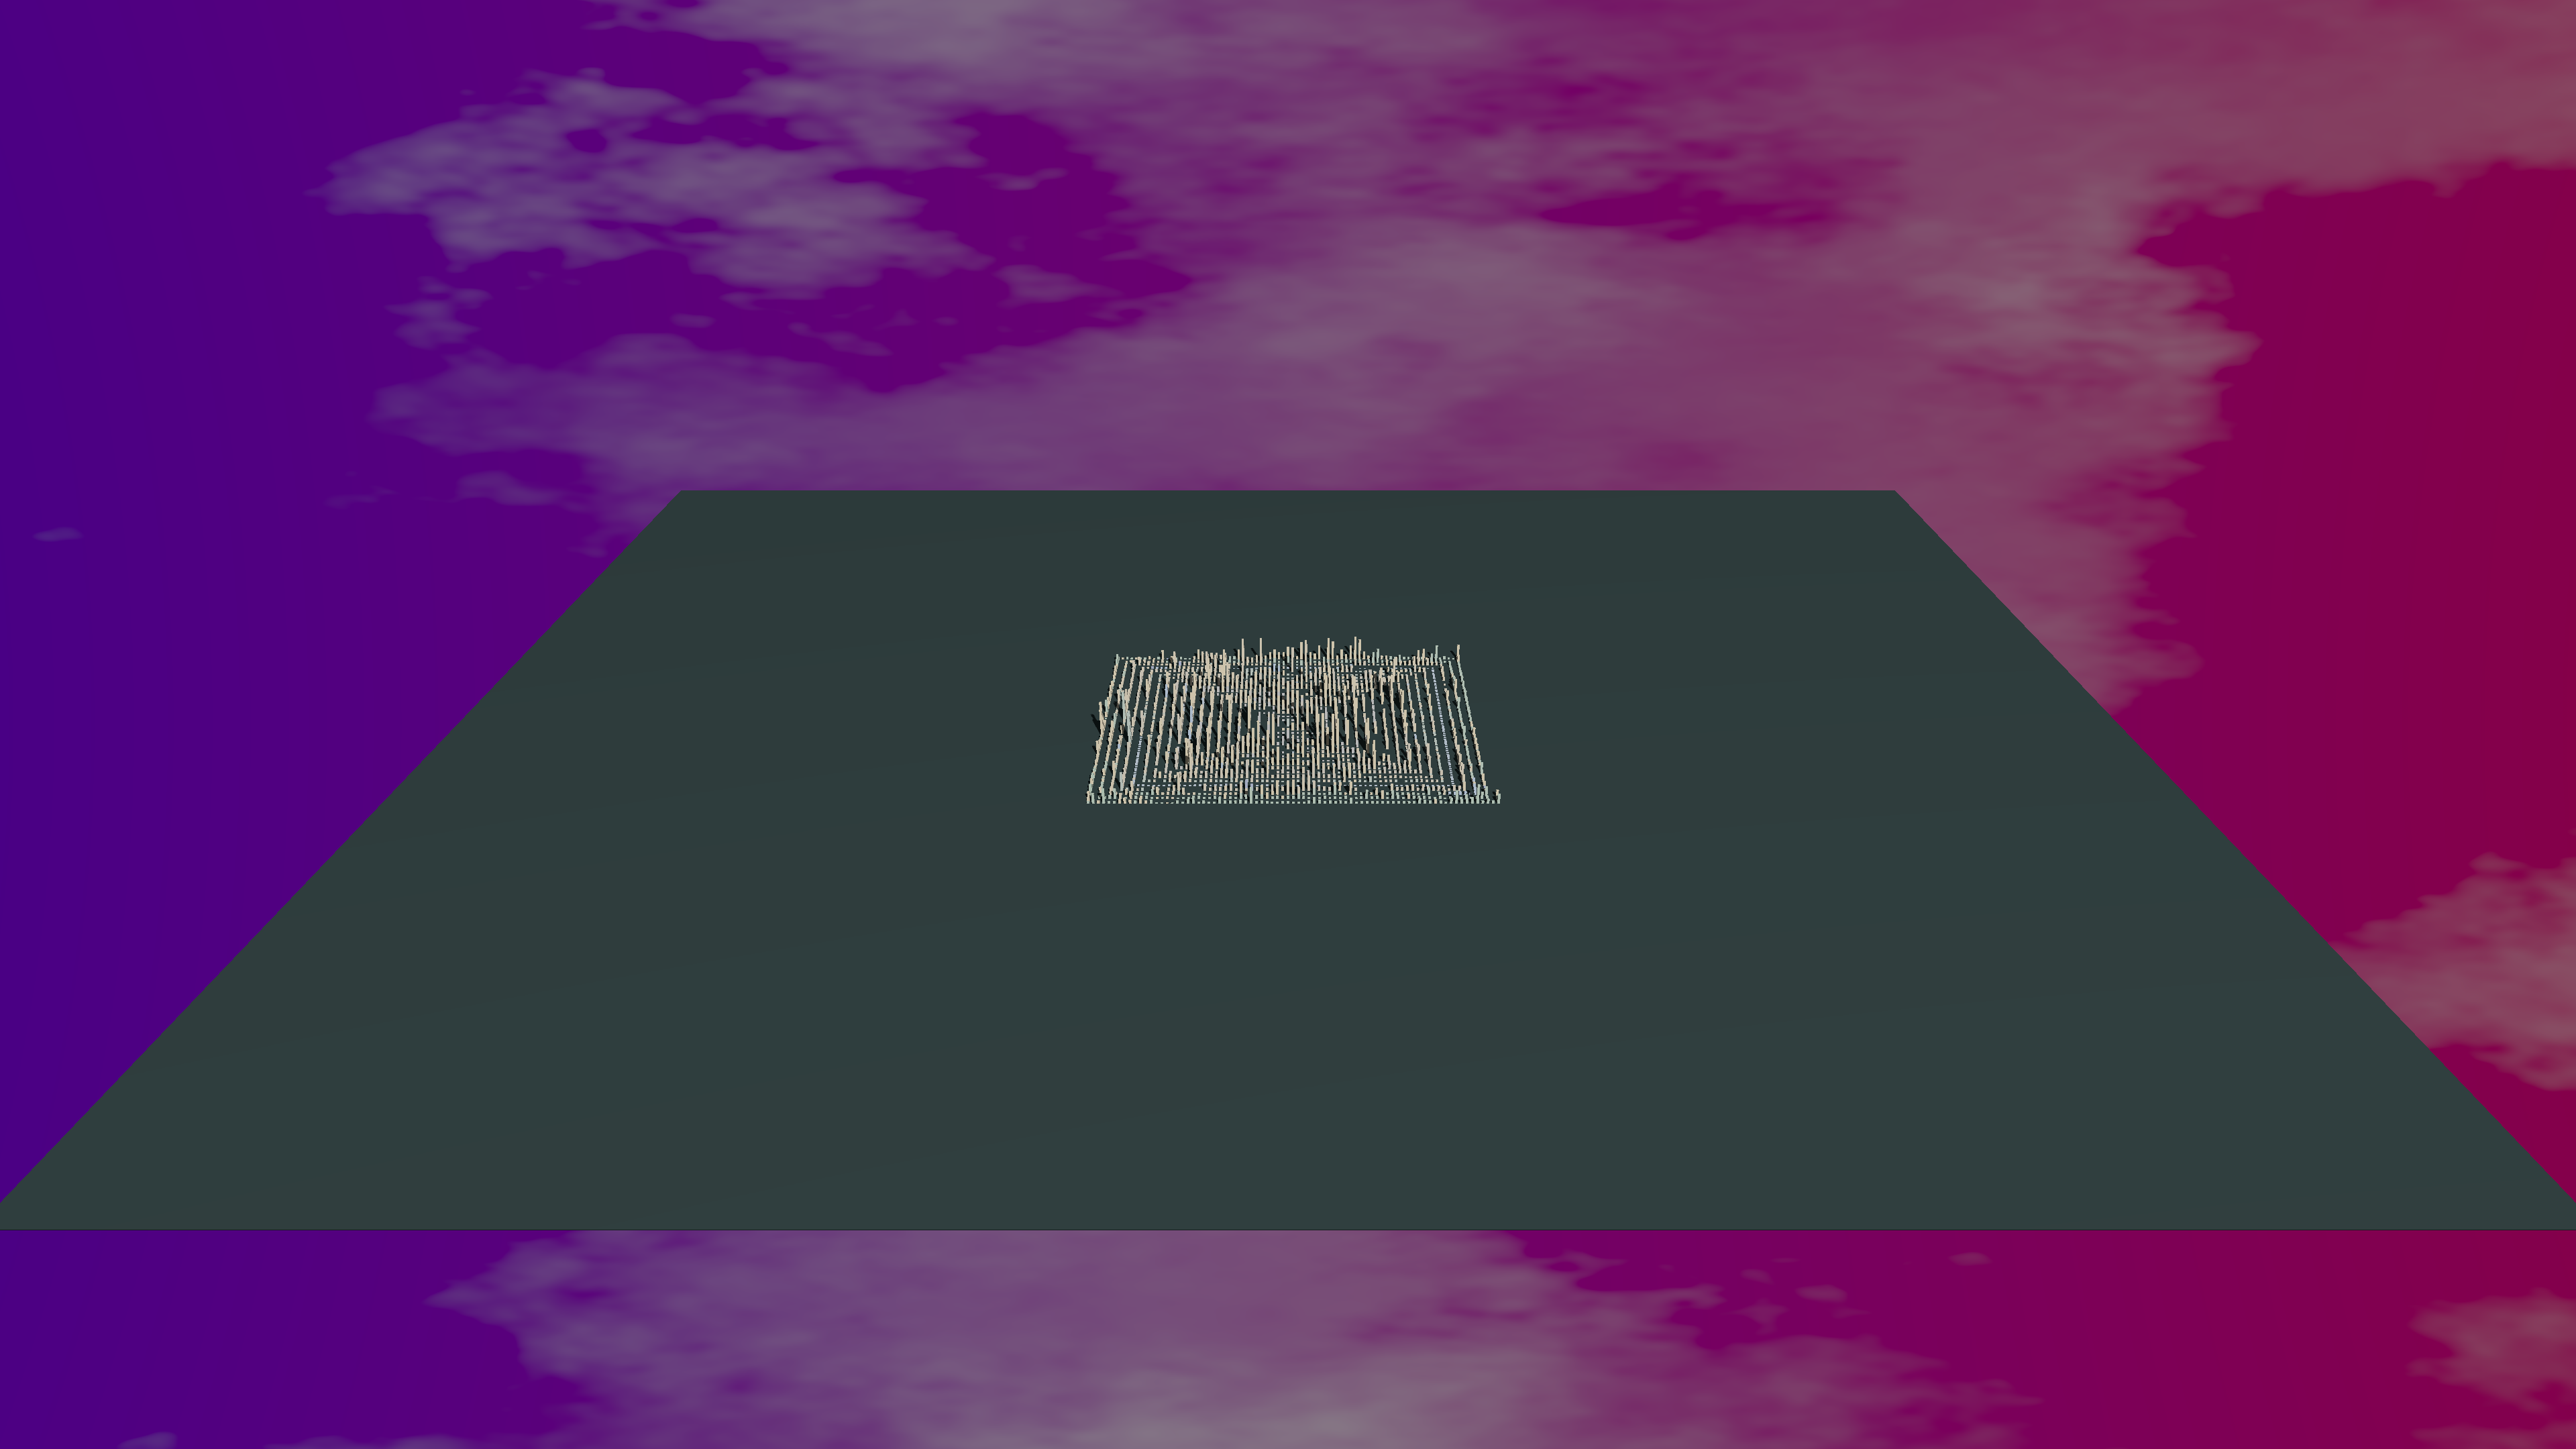
\includegraphics[width=\linewidth]{Elasticsearch/Animation001.png}
        \caption{Elasticsearch in June 2014 (1 year)} 
        \label{fig:Elastic_V5_S1}
    \end{subfigure}\hspace*{\fill}
    \begin{subfigure}{0.48\textwidth}
        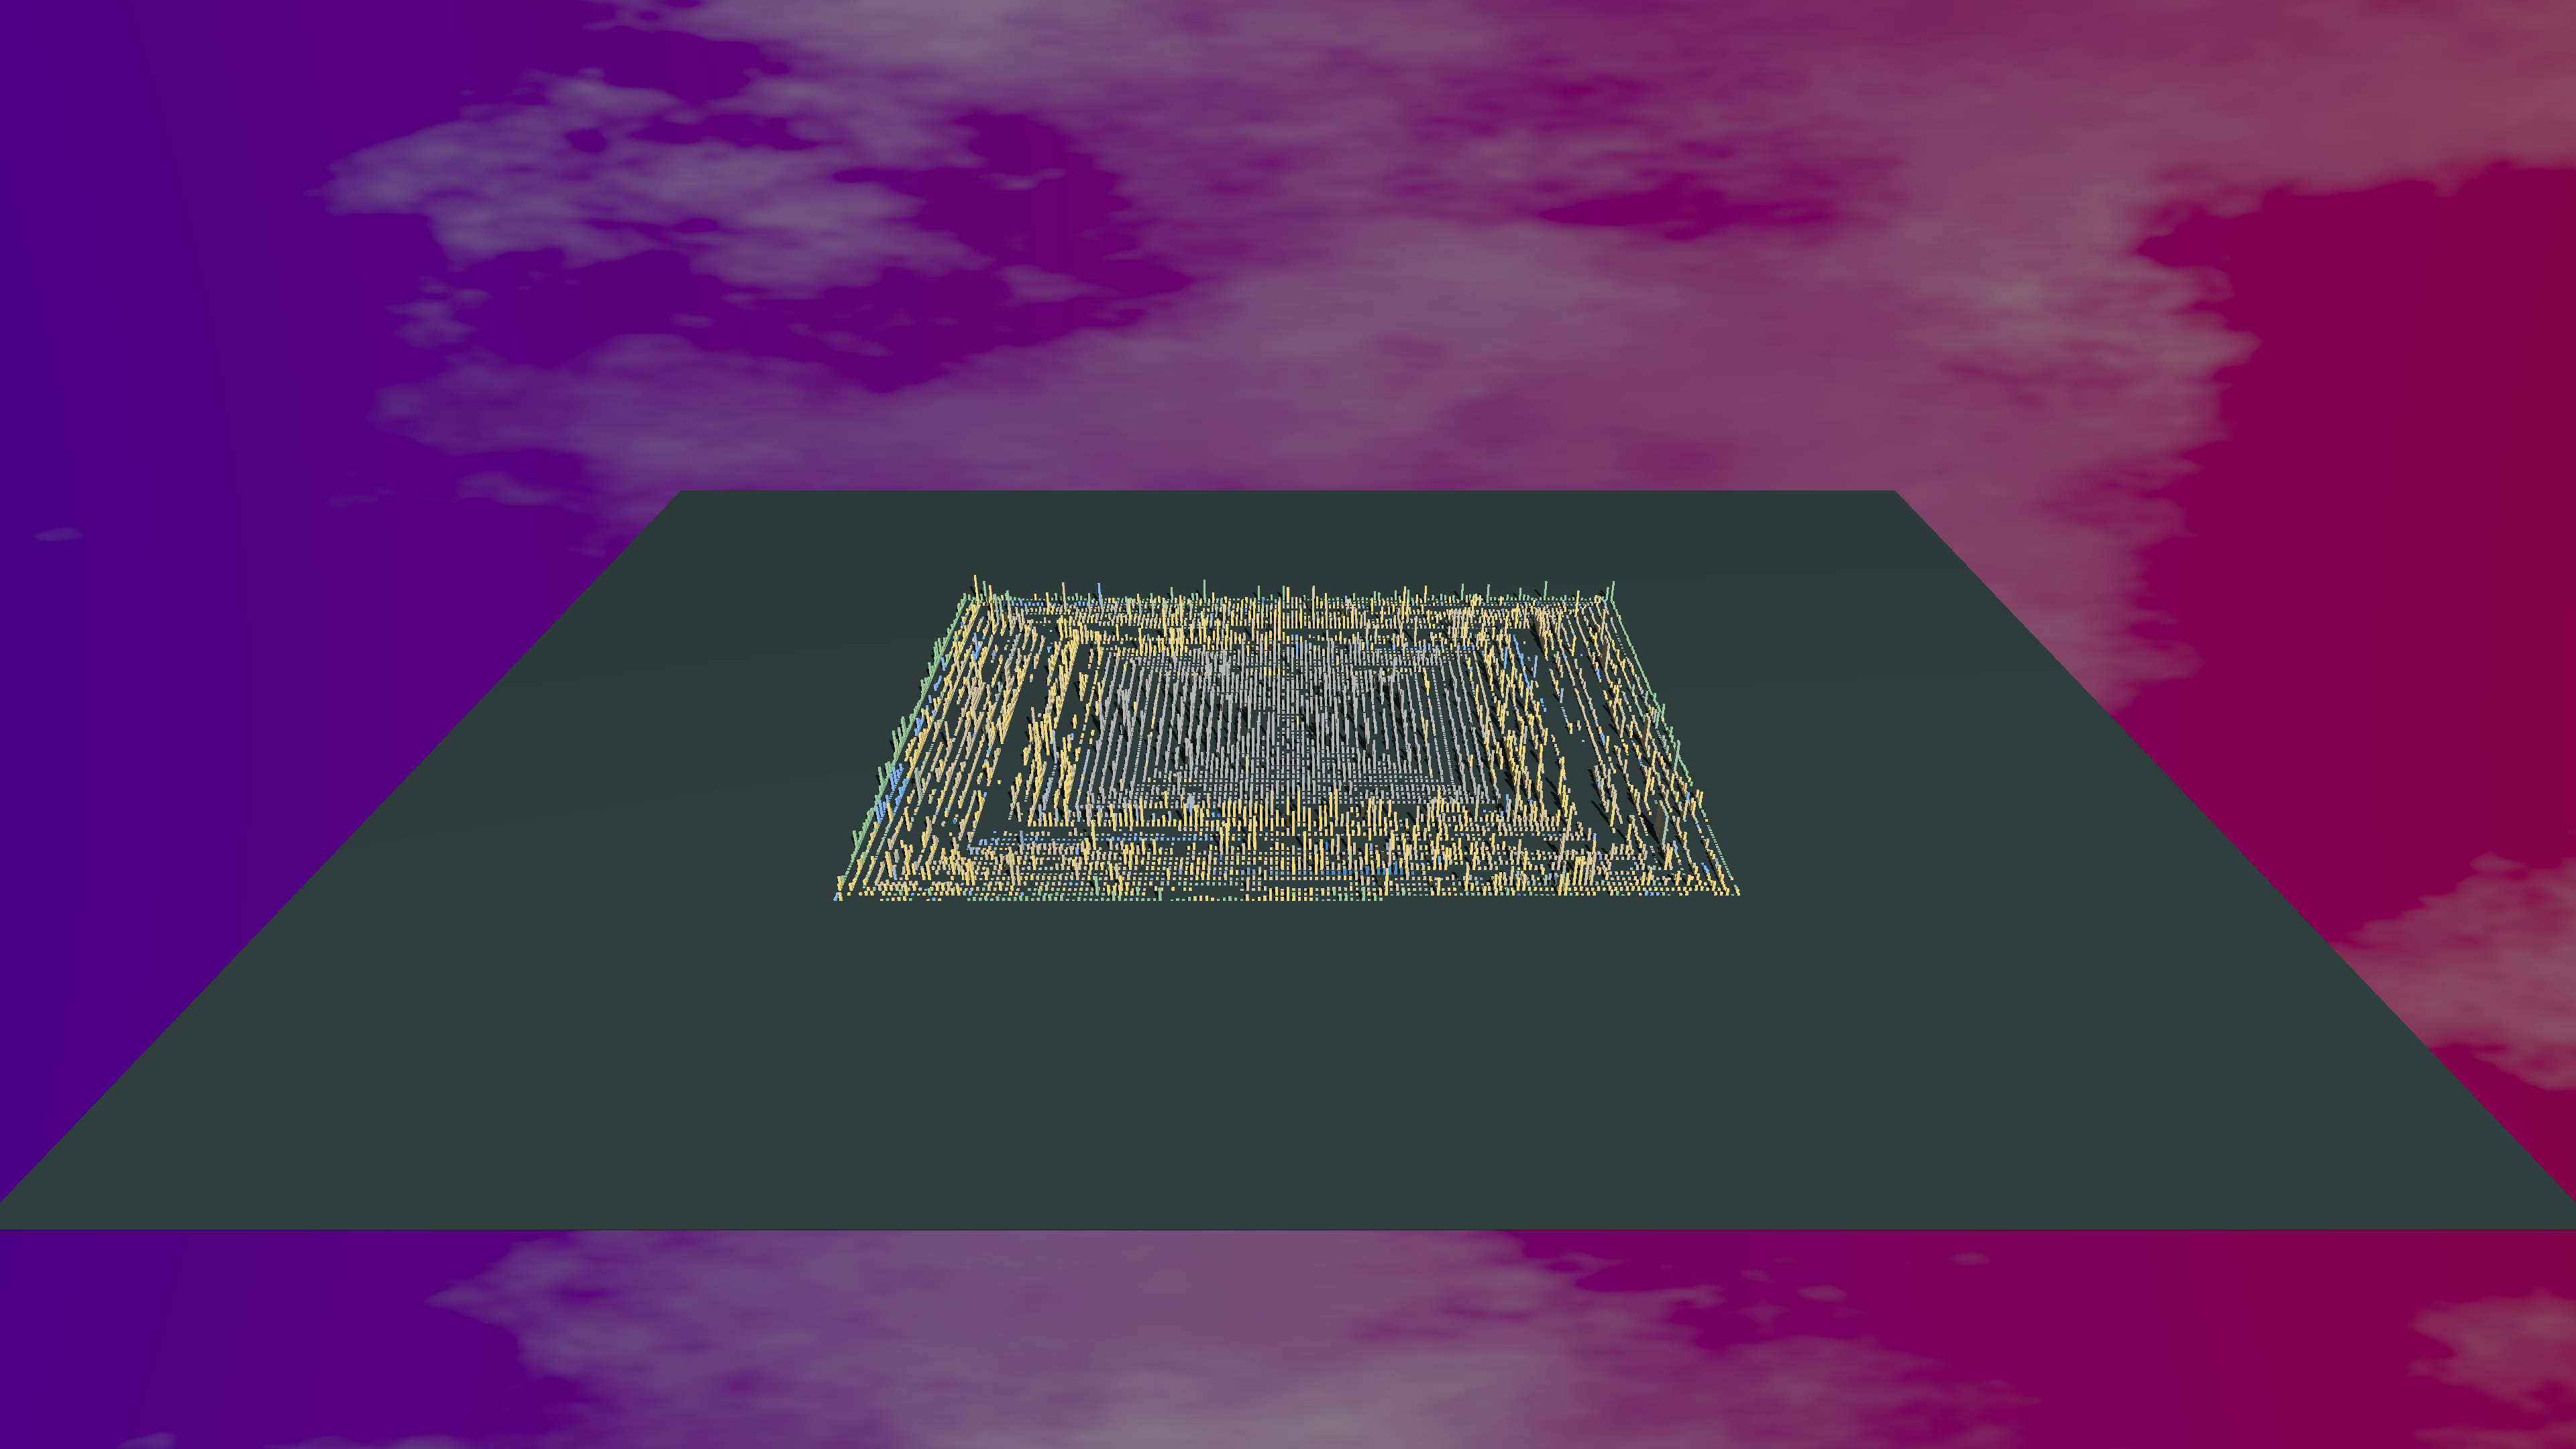
\includegraphics[width=\linewidth]{Elasticsearch/Animation003.png}
        \caption{Elasticsearch in June 2016 (3 year)} 
        \label{fig:Elastic_V5_S2}
    \end{subfigure}
    \medskip
    \begin{subfigure}{0.48\textwidth}
        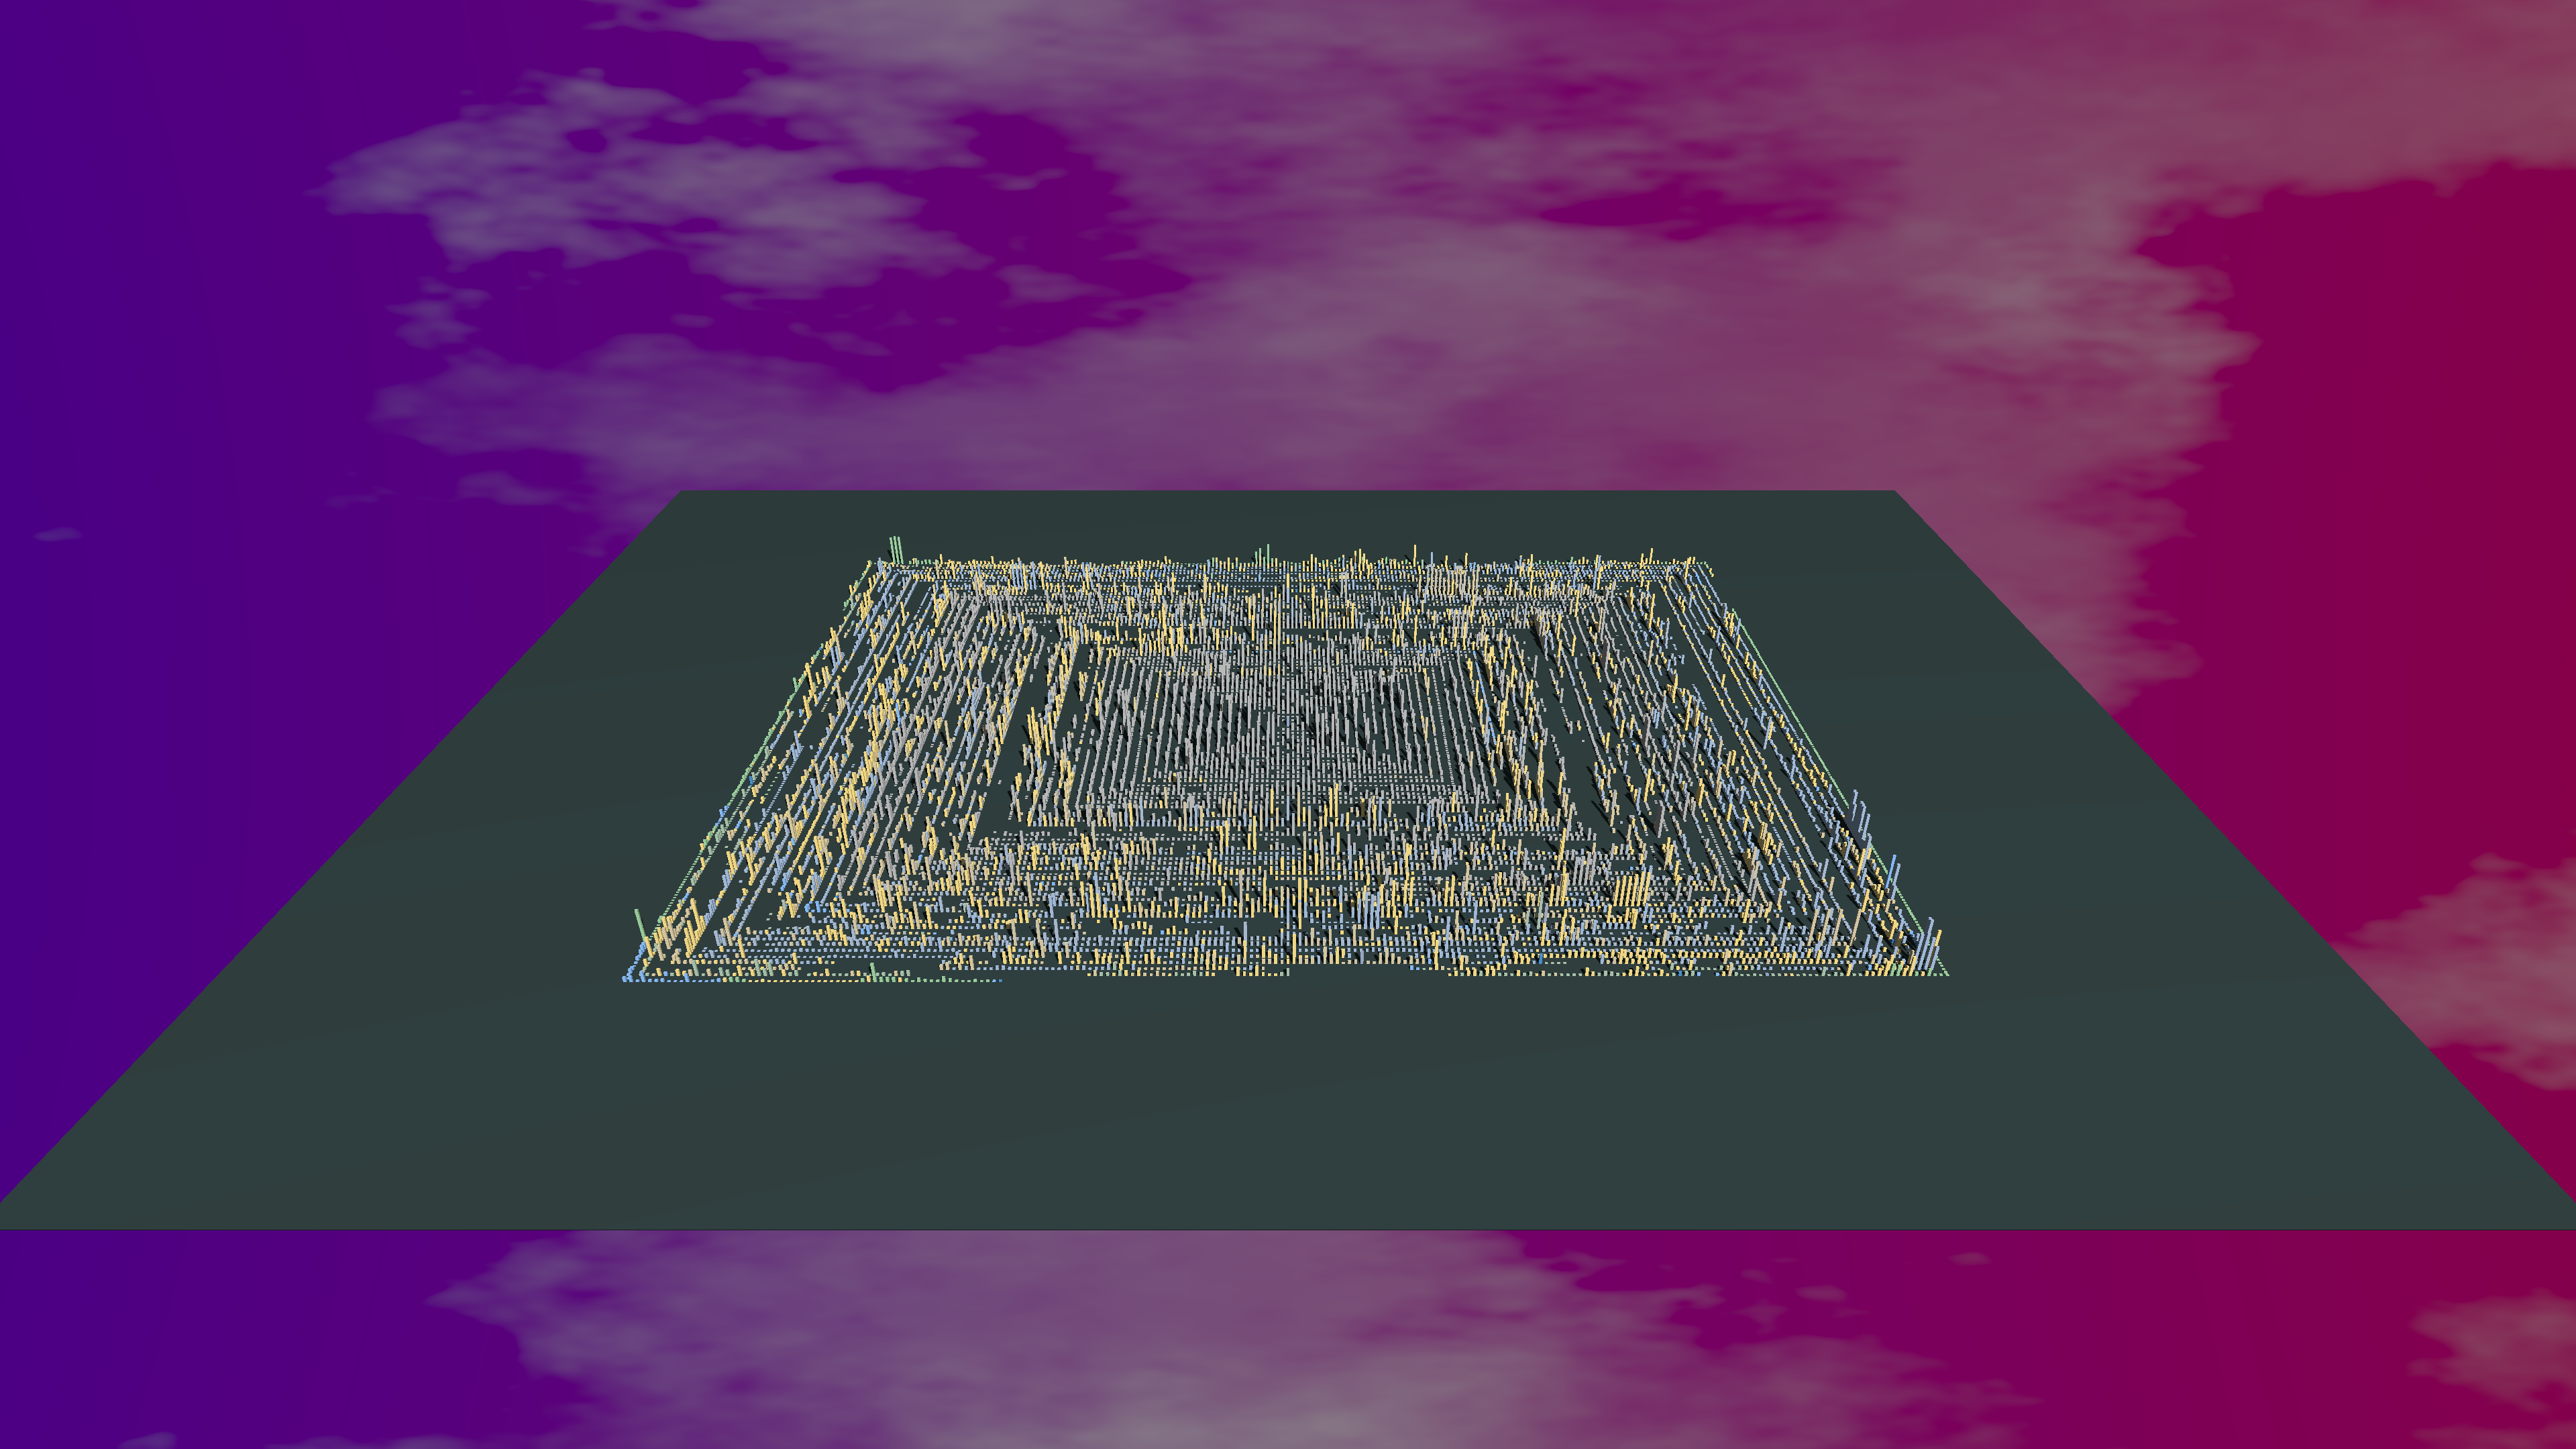
\includegraphics[width=\linewidth]{Elasticsearch/Animation005.png}
        \caption{Elasticsearch in June 2018 (5 year)} 
        \label{fig:Elastic_V5_S3}
    \end{subfigure}\hspace*{\fill}
    \begin{subfigure}{0.48\textwidth}
        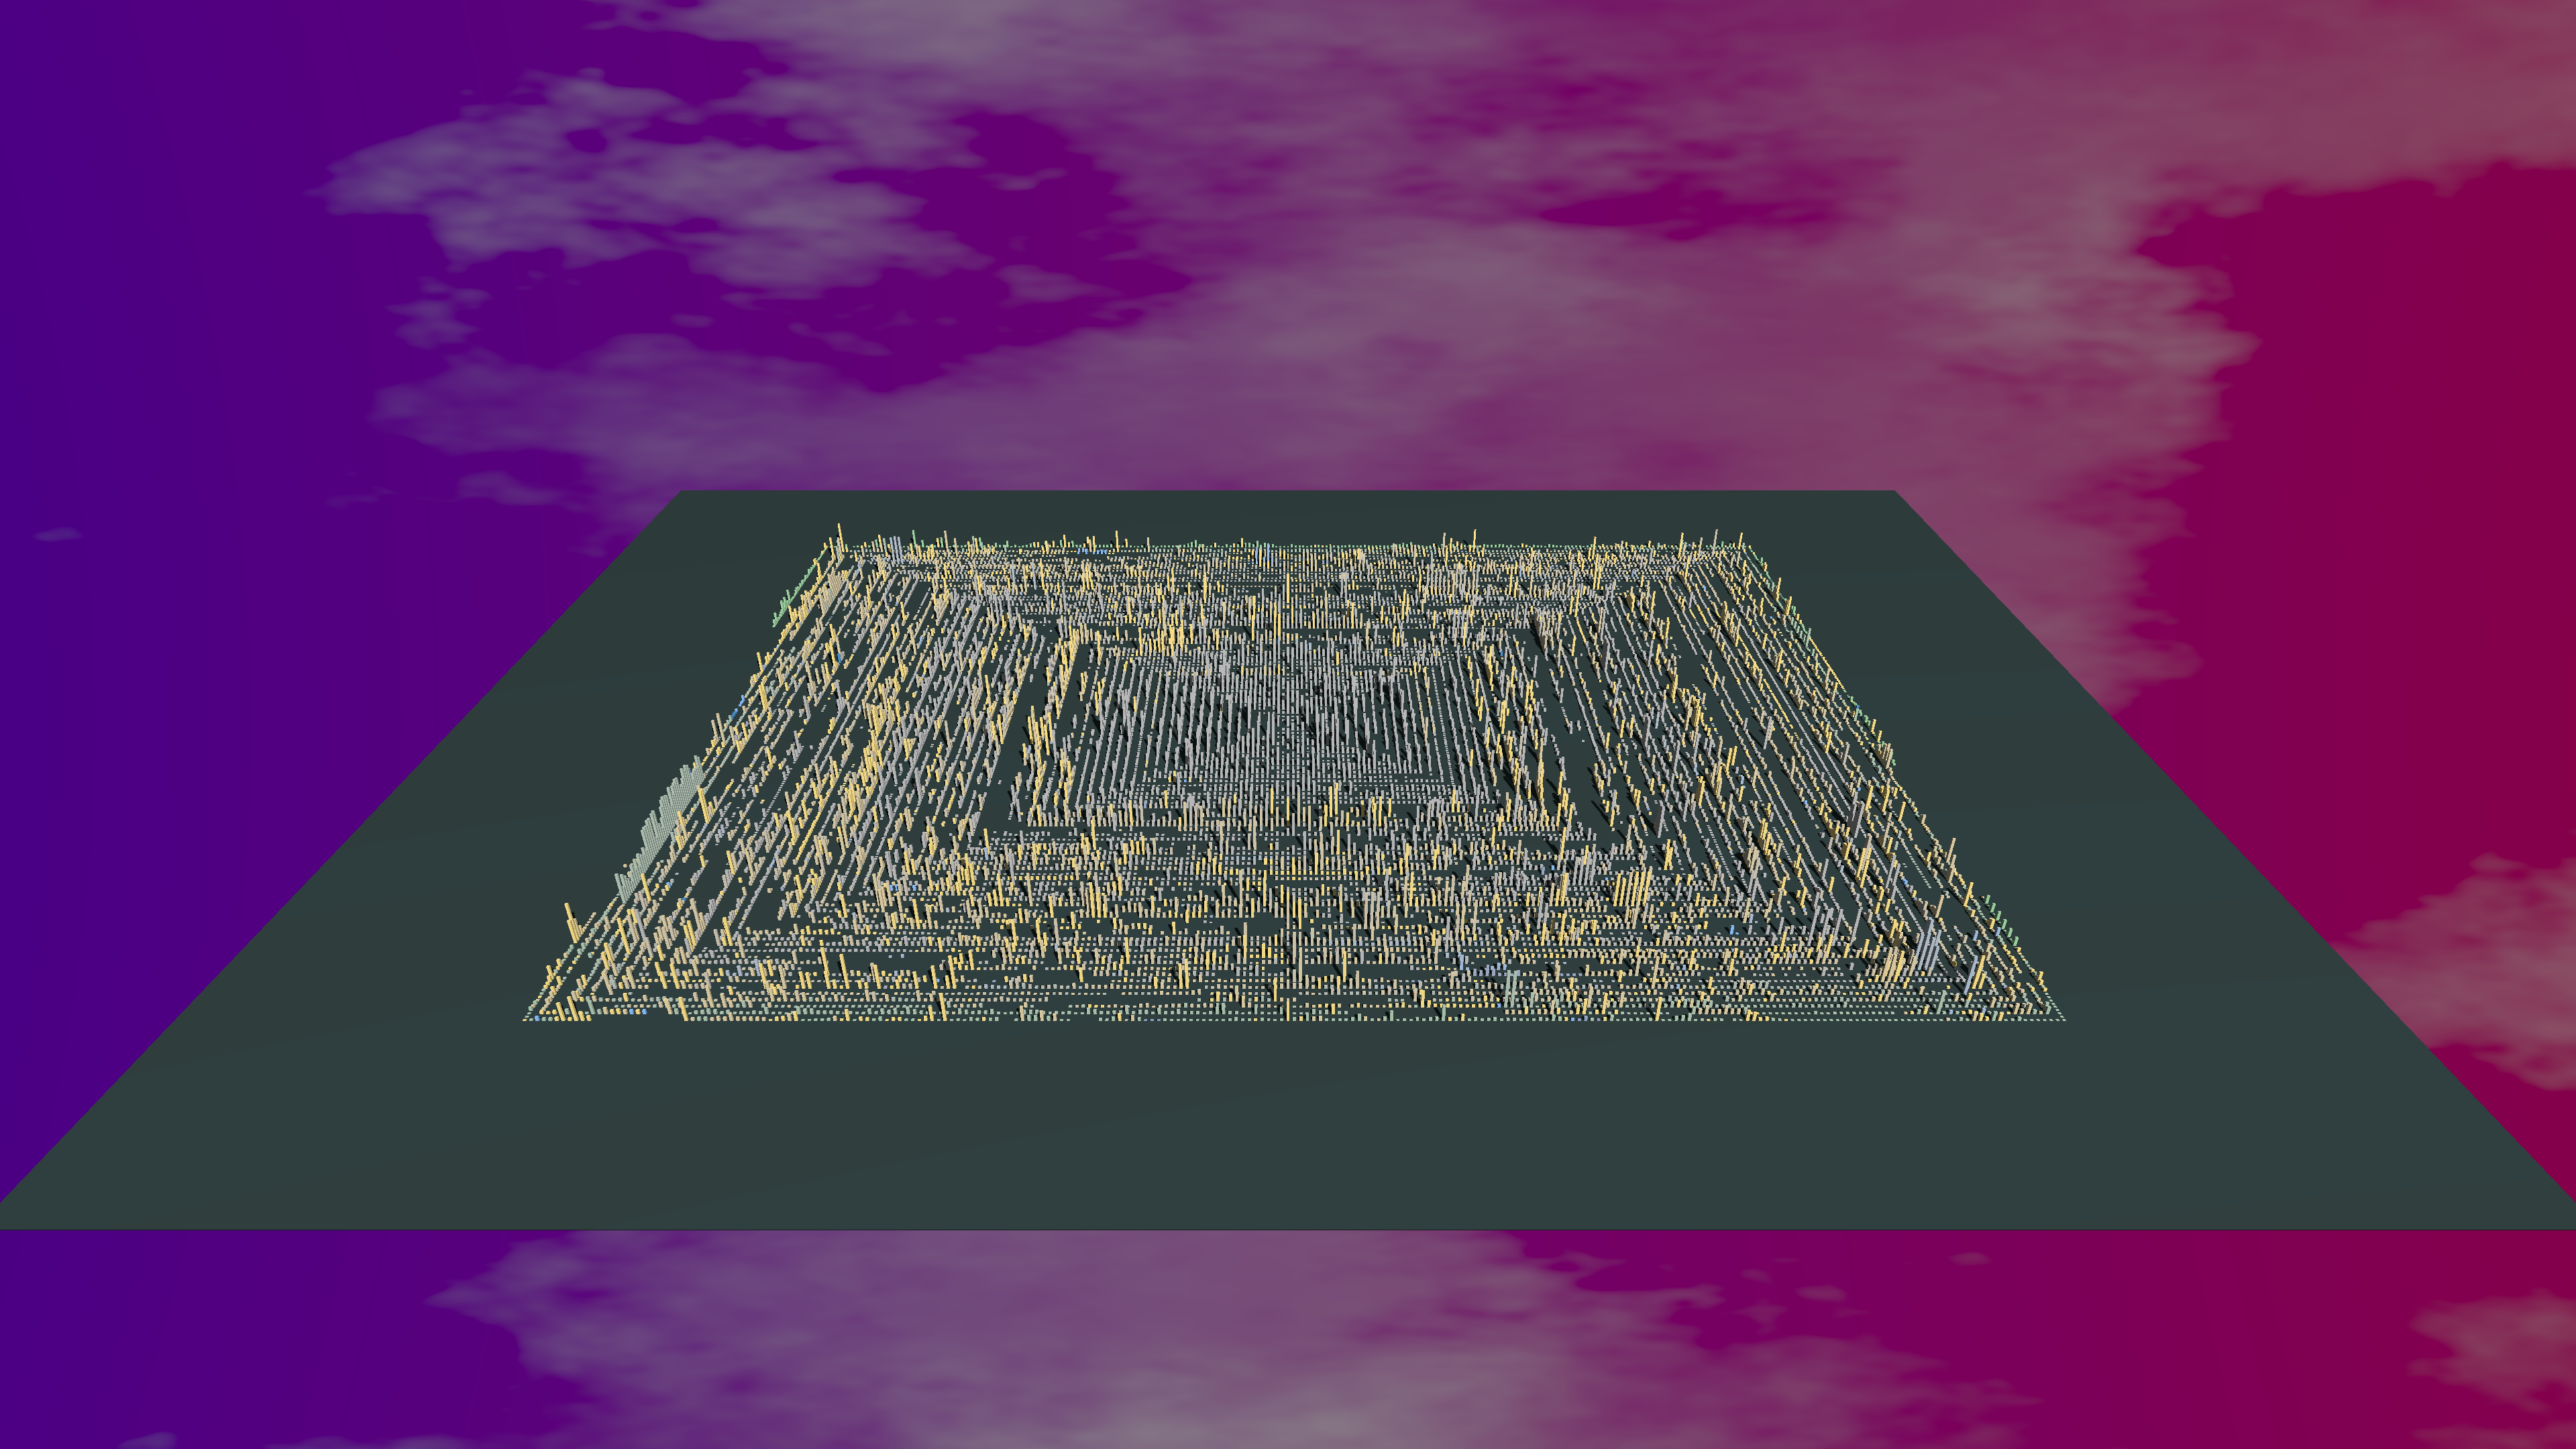
\includegraphics[width=\linewidth]{Elasticsearch/Animation006.png}
        \caption{Elasticsearch in June 2019  (6 year)} 
        \label{fig:Elastic_V5_S4}
    \end{subfigure}
    \medskip
    \begin{subfigure}{0.48\textwidth}
        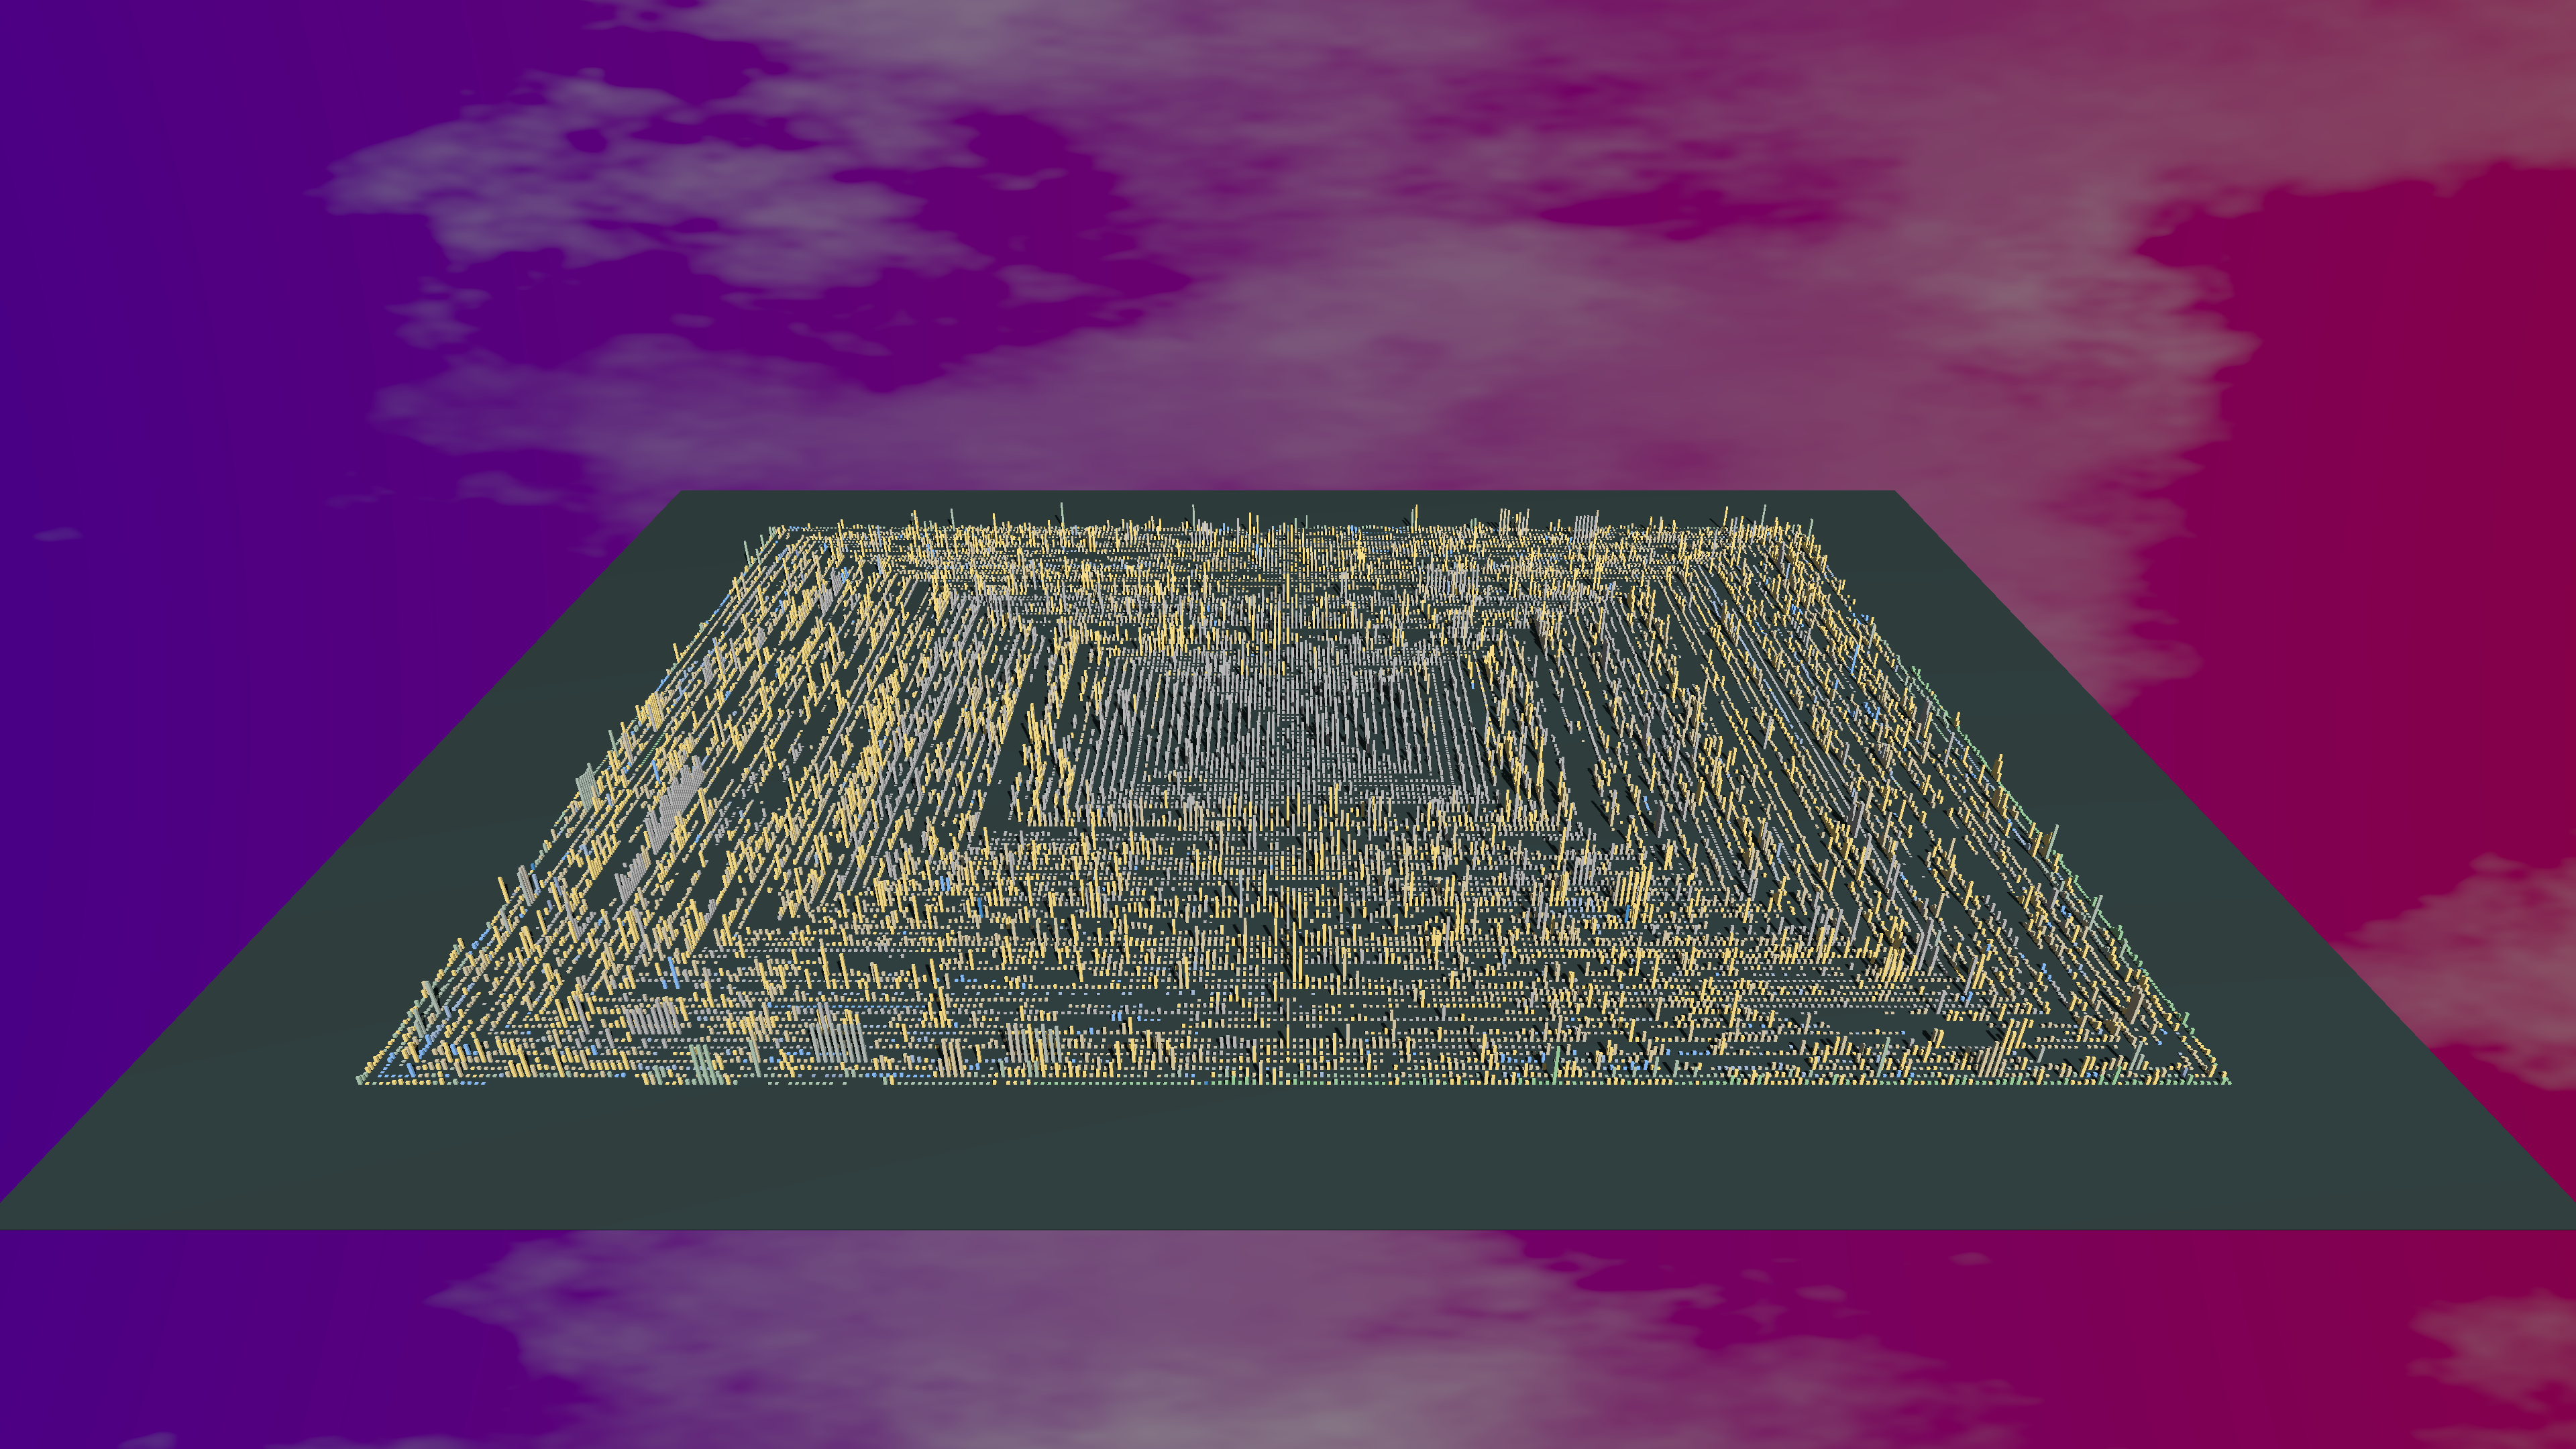
\includegraphics[width=\linewidth]{Elasticsearch/Animation008.png}
        \caption{Elasticsearch in June 2021 (8 year)} 
        \label{fig:Elastic_V5_S5}
    \end{subfigure}\hspace*{\fill}
    \begin{subfigure}{0.48\textwidth}
        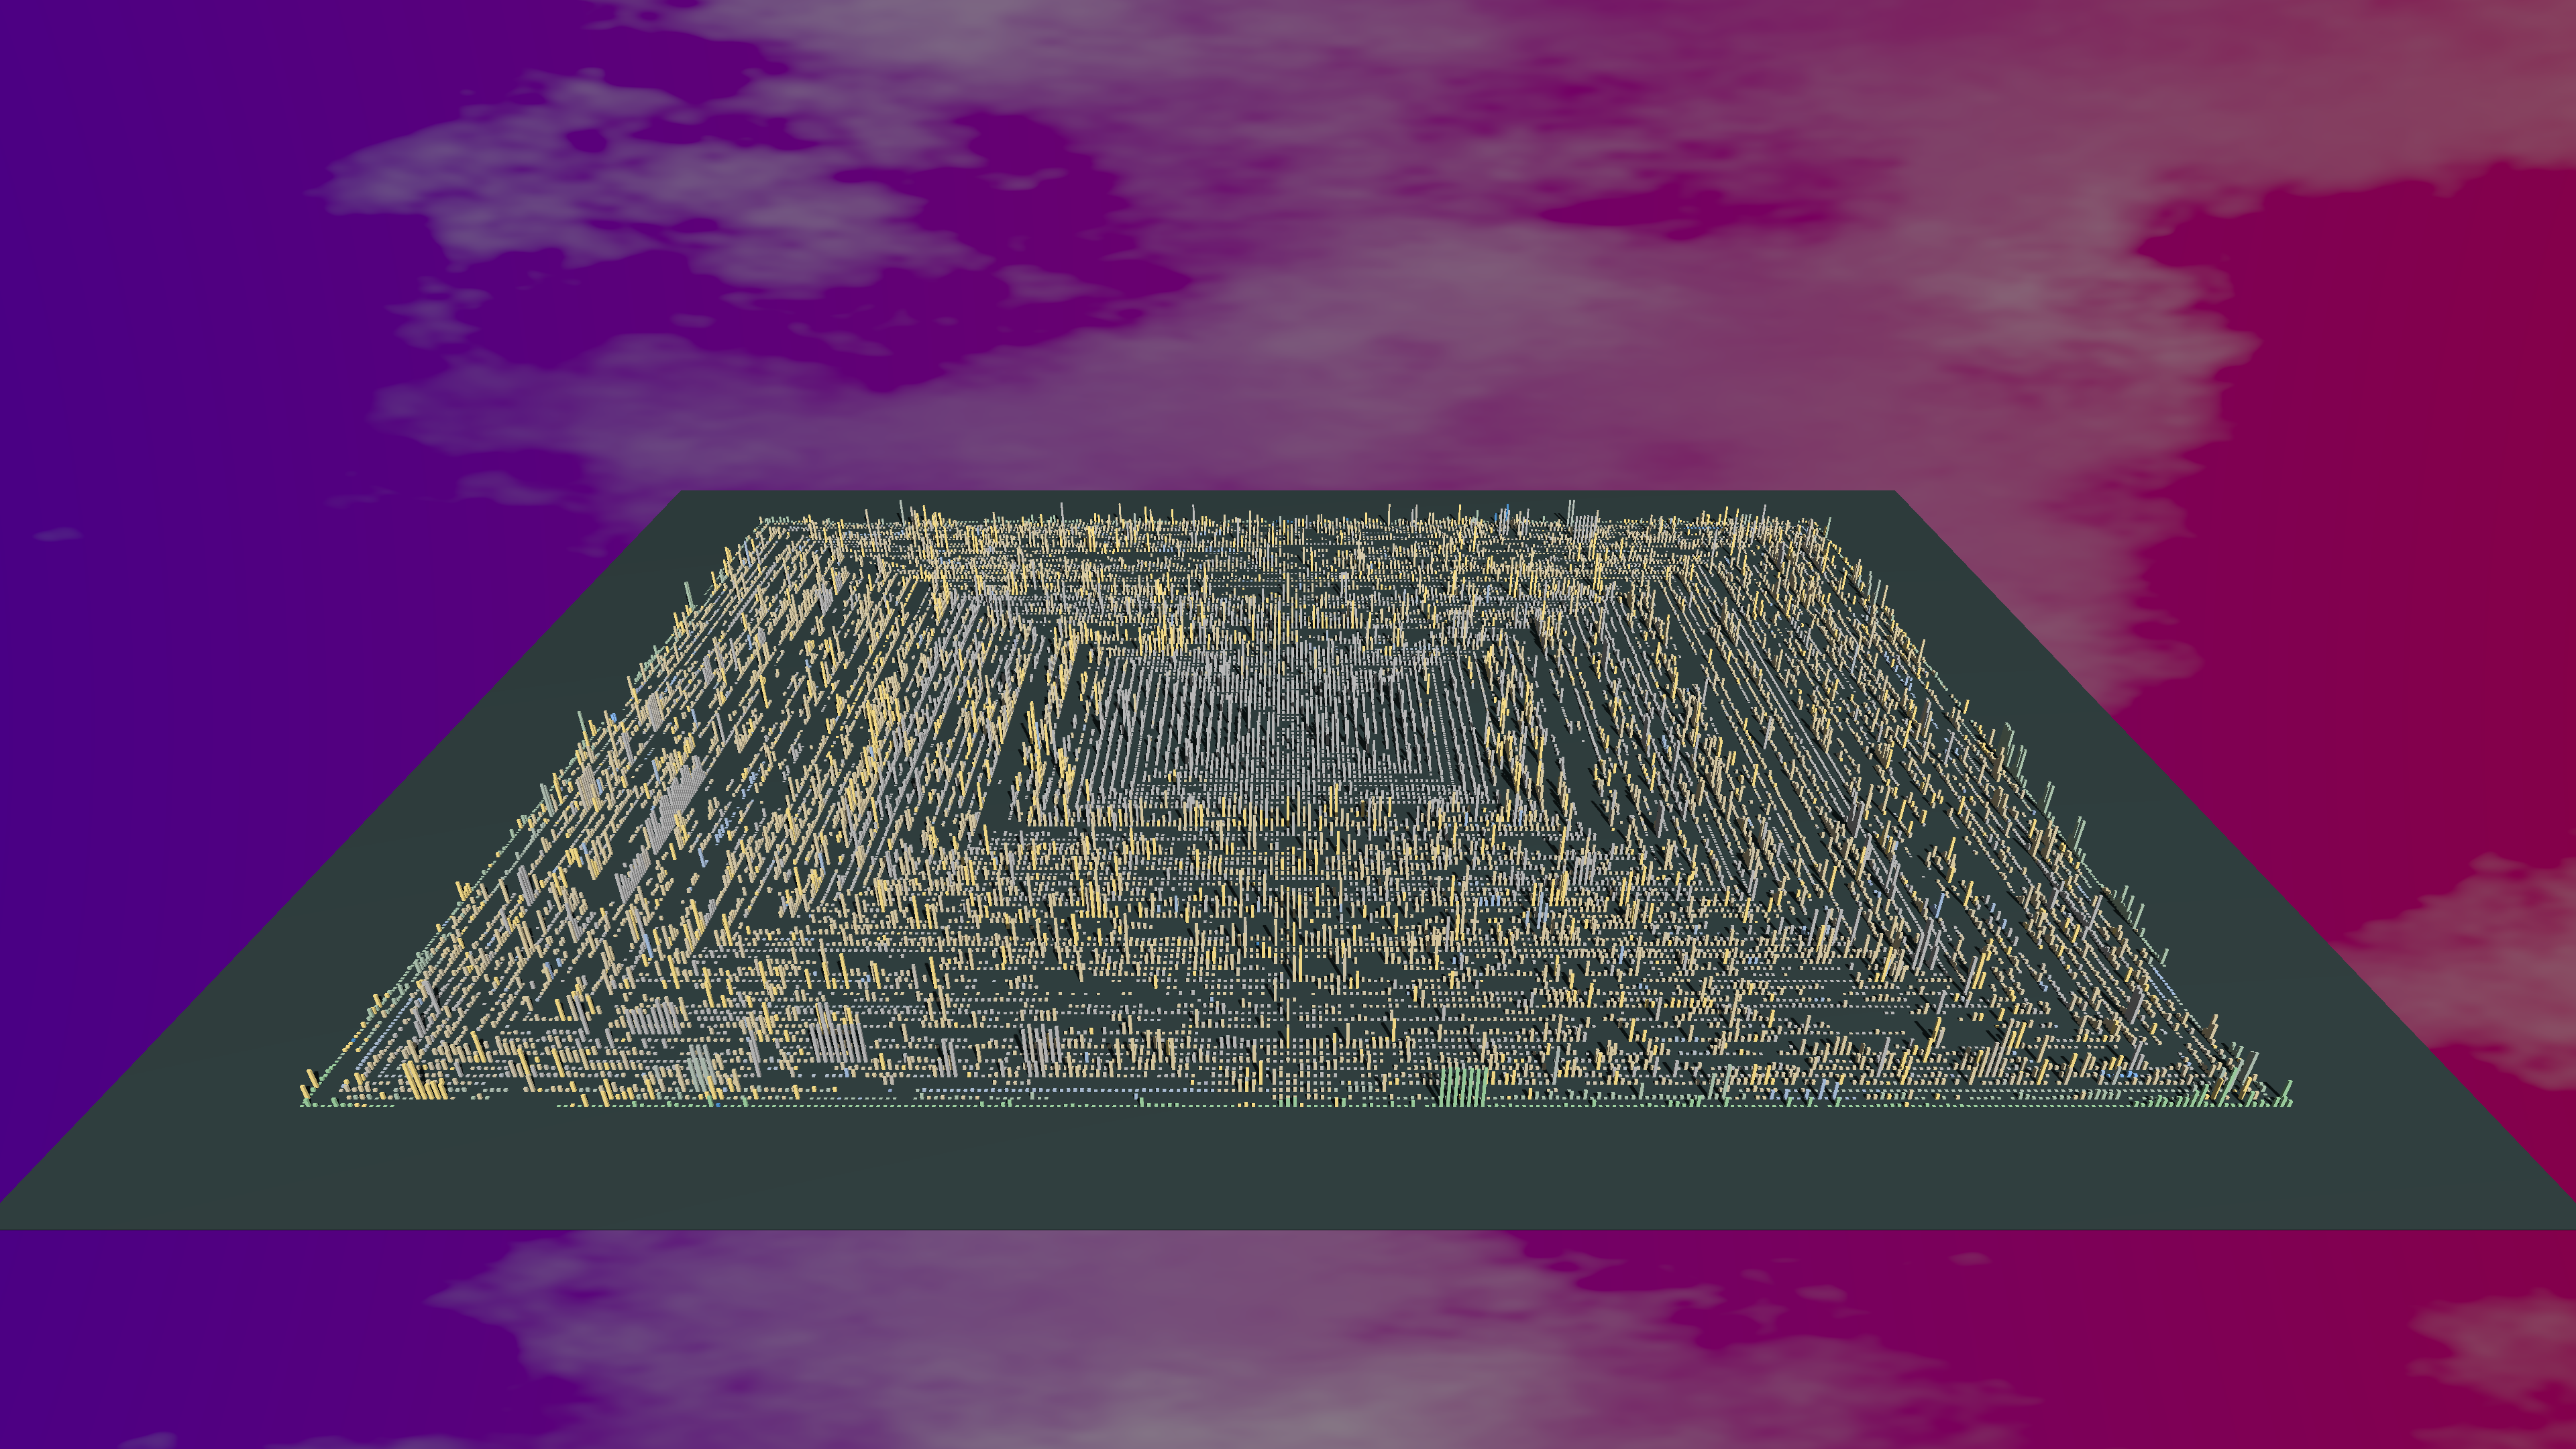
\includegraphics[width=\linewidth]{Elasticsearch/Animation009.png}
        \caption{Elasticsearch in June 2022 (9 year)} 
        \label{fig:Elastic_V5_V3S6}
    \end{subfigure}
    
    \caption{Hot spots during the evolution of Elasticsearch} 
    \label{fig:Elastic_V5}
\end{figure}


% -------------------------------------------
% libreoffice
% FileHistories: 213791 
% ProjectVersions: 367996 
% FileVersions: 1924183 
% First Version: 
% 	 hash: 5acbb755f3f8dedf51904b711ff78f5e1aa498cf 
% 	 date: Thu Mar 07 16:45:23 CET 2002 
% Last Version: 
% 	 hash: 634f13a722dc68b7a2df7518880ce4f9d5d89f19 
% 	 date: Sat Jun 18 16:10:53 CEST 2022 
% Diff: {DAYS=107, HOURS=22, MINUTES=25, SECONDS=30, MILLISECONDS=0, MICROSECONDS=0, NANOSECONDS=0, YEARS=20}
% -------------------------------------------
\clearpage
\section{Libreoffice}
LibreOffice is an integrated office suite compatible with most document formats and standards. Its first commit \footnote{\url{https://github.com/LibreOffice/core/commit/5acbb755f3f8dedf51904b711ff78f5e1aa498cf}}, made on 07 March 2002 was an import of the original codebase developed by Sun Microsystems. The repository's history is 20 years long with 327'996 commits, 213'791 FileHistories, and almost 2M FileVersions. 

%\subsection{View 6}
\textbf{Goal of this visualization}
This visualization aims to see how the repository evolved through its last 20 years. We decided to adopt a commit grouping strategy based on a time window of 1 year and an aging strategy of one month with 12 steps. Hence, grey entities represent files that have not been updated for more than 12 months. 

\bigbreak
View specification adopted: same as the one defined for the View 4 (\autoref{subsec:view4}).

\textbf{Results}
Here we present only the relevant aspects of the ArgoUML evolution that we have found. However, the full evolution is depicted in \autoref{app:Libre_Evolution}. \autoref{fig:Libre_V6} shows the hot spots during the system's evolution. The initial composition of the system is shown in \autoref{fig:Libre_V6_S1}. Between 2003 and 2011, the system 
grew substantially: if on March 2003, it had 13'500 files, and in March 2011, it had 57'520 files with an increment of over 40K files. \autoref{fig:Libre_V6_S2} shows the state of the repository in March 2011. Few entities are painted with a color, meaning that only a few parts of the codebase were touched. \autoref{fig:Libre_V6_S3} shows the state in March 2012. Closely to that date, the repository was involved in a big refactoring where most of the recently added files were moved. Moreover, in this picture, we initially start to see empty rings like the ones we saw in the analysis of ArgoUML. Another important aspect of this picture is that the core was entirely modified. As we can see, it is colored yellow, and the entities are taller than the year before. The work on the repository was constant until June 2022. In all the AnimationFrames, the center was always painted with yellow colors. This could mean that the core still needs maintenance after 20 years of the recently developed features heavily relying on the core implementation, and thus it needs to be adapted. In the last 12 years, as it can be seen from \ref{fig:Libre_V6_S4}, \ref{fig:Libre_V6_S5} and \ref{fig:Libre_V6_S6} the system doubled its size. In June 2022, it counted 135'793 files. Moreover, empty rings around the core became thicker, suggesting the deletion of a whole part of the system that it might be reimplemented later.

\bigbreak
\textbf{Conclusion} As we saw from this analysis, the evolution of LibreOffice was constant throughout its 20 years of history. 
Thanks to the aging concept of SYN, we understood that they heavily rely on code that was added 20 years ago. The core of the system was constantly updated, and the overall size of entities the highest area in the middle. The empty bands around the core represent a pattern that we have already recognized in ArgoUML. It means that a set of files were removed one after another. Perhaps these files might be an entire folder that contained a feature that was later readded. One issue that this visualization raised is the size of the system that begins visualized with this approach. It is hard to infer the color of some entities since they are too small to be individually identified. 

\begin{figure}[ht]
    \begin{subfigure}{0.48\textwidth}
        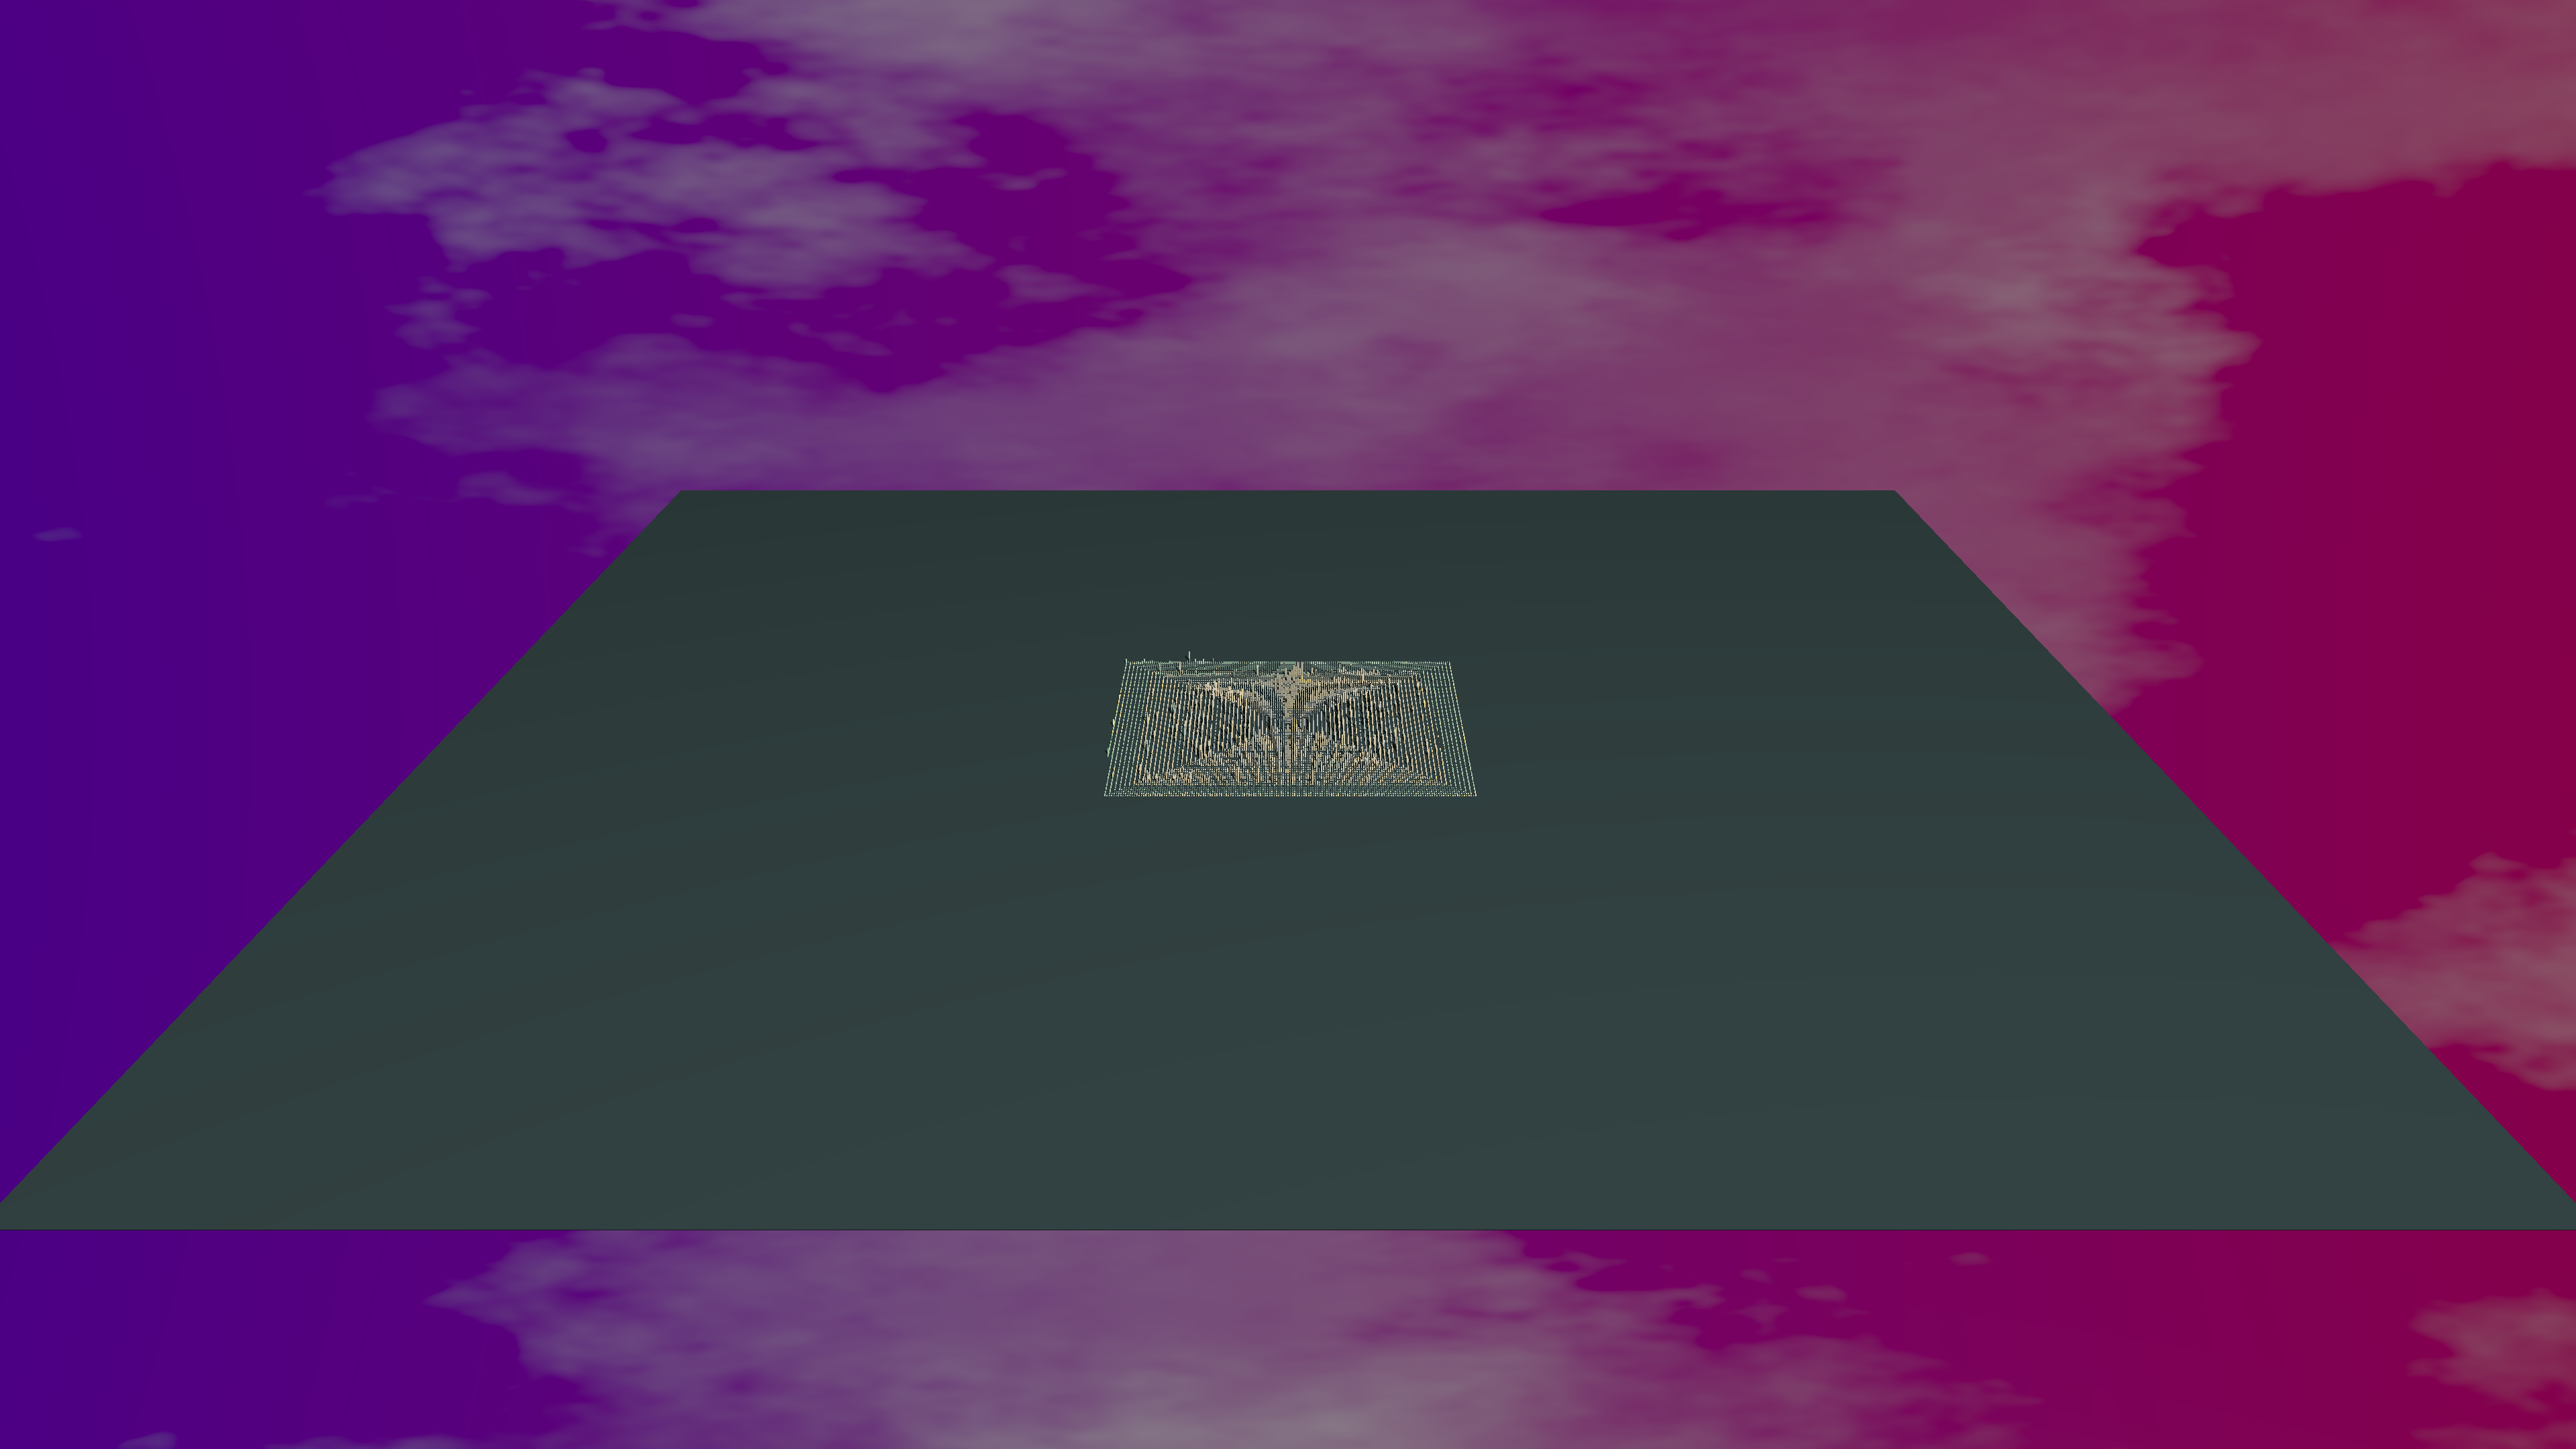
\includegraphics[width=\linewidth]{Libreoffice/Animation001.png}
        \caption{Libreoffice in March 2003 (1 year)} 
        \label{fig:Libre_V6_S1}
    \end{subfigure}\hspace*{\fill}
    \begin{subfigure}{0.48\textwidth}
        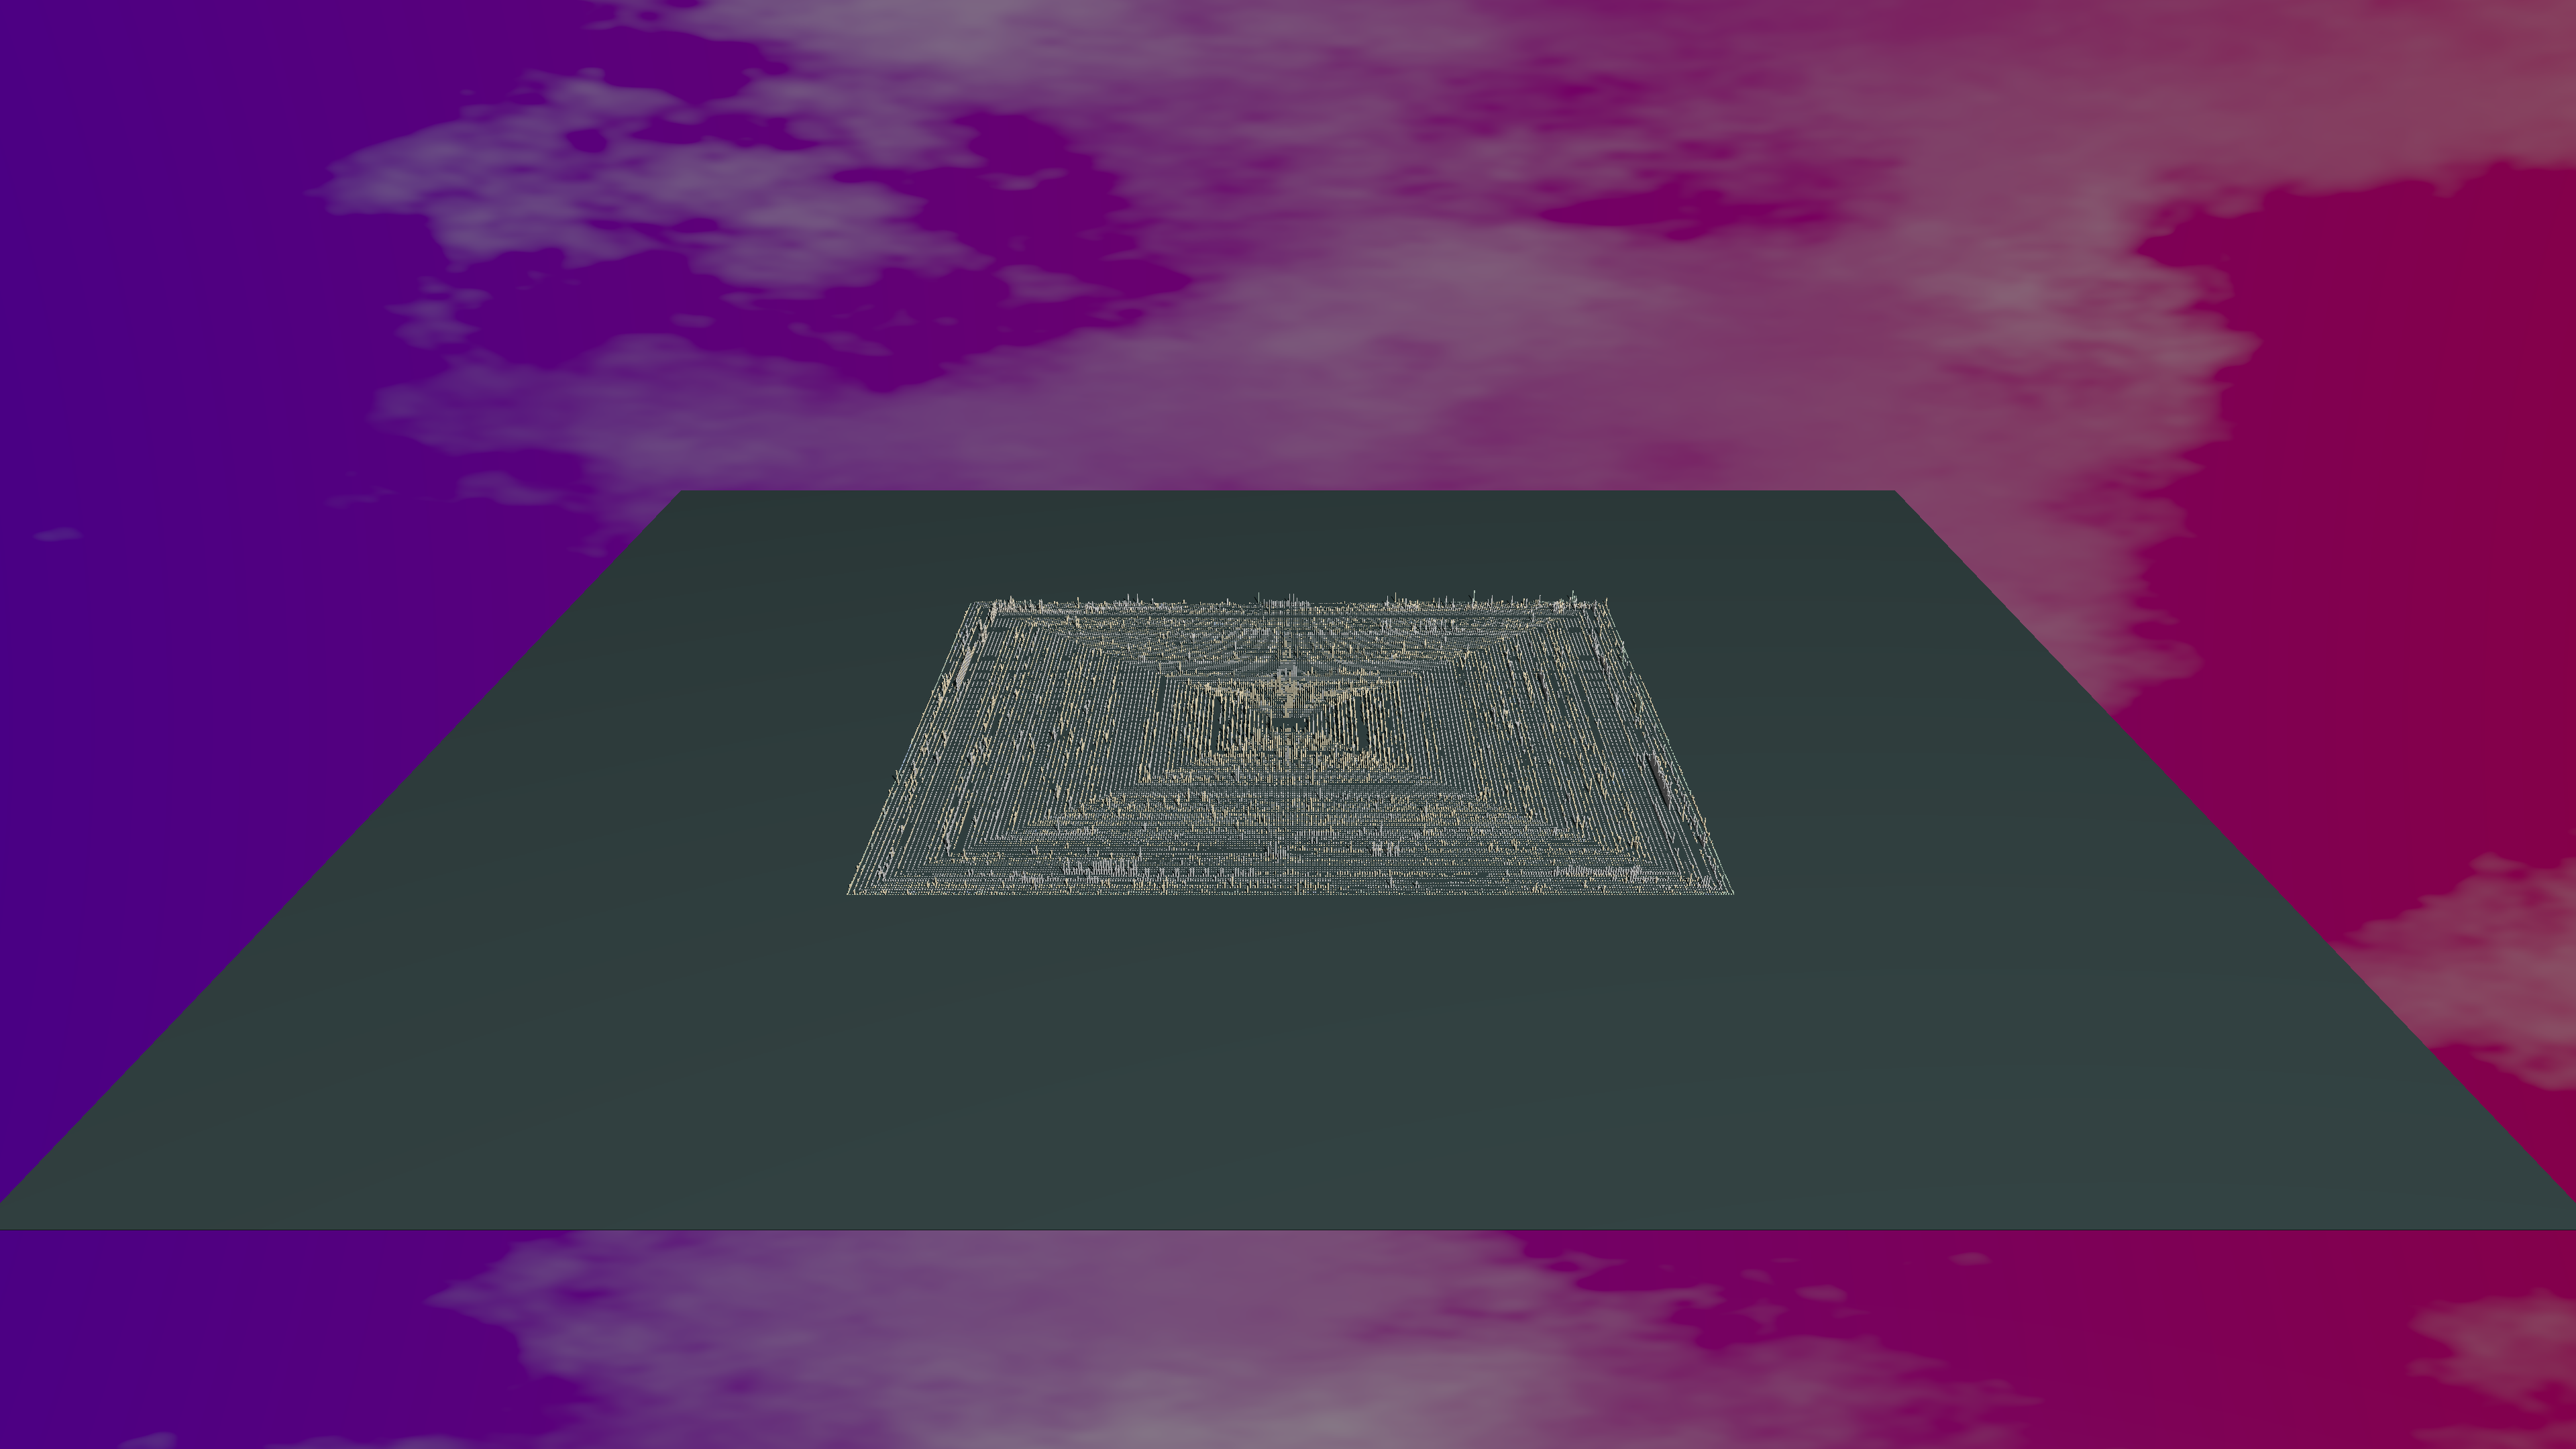
\includegraphics[width=\linewidth]{Libreoffice/Animation009.png}
        \caption{Libreoffice in March 2011 (9 year)} 
        \label{fig:Libre_V6_S2}
    \end{subfigure}
    \medskip
    \begin{subfigure}{0.48\textwidth}
        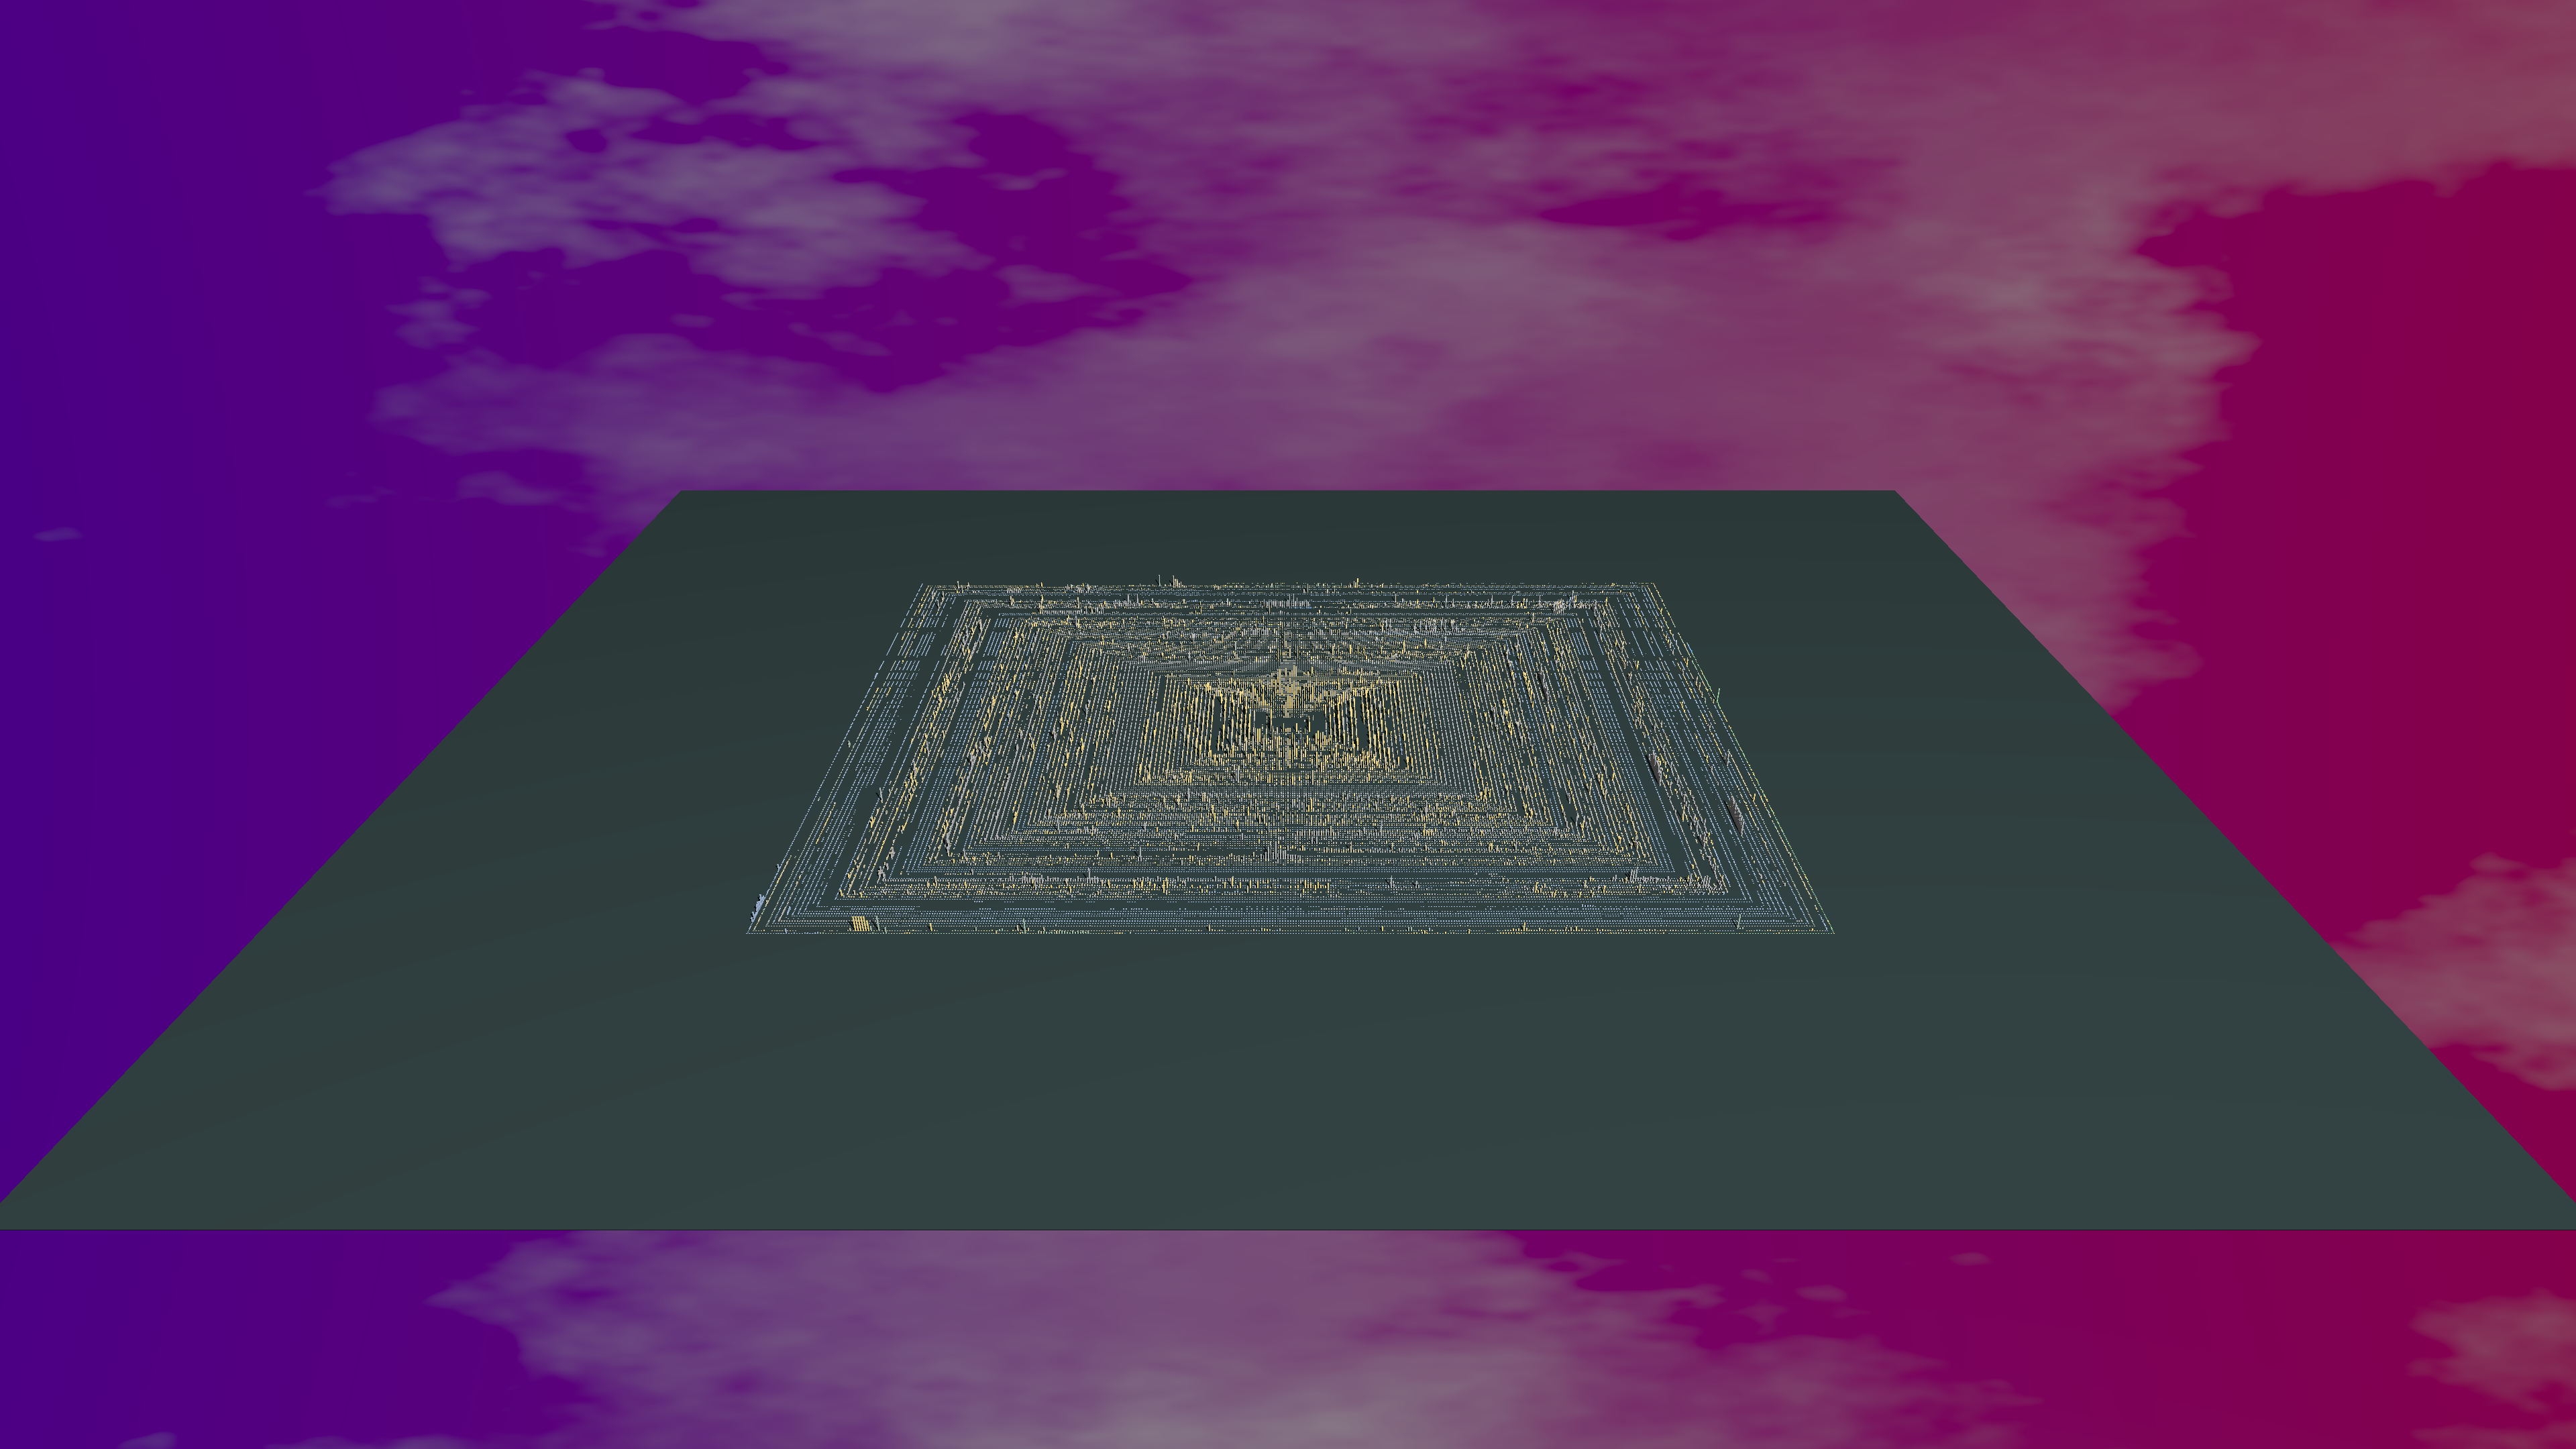
\includegraphics[width=\linewidth]{Libreoffice/Animation010.png}
        \caption{Libreoffice in March 2012 (10 year)} 
        \label{fig:Libre_V6_S3}
    \end{subfigure}\hspace*{\fill}
    \begin{subfigure}{0.48\textwidth}
        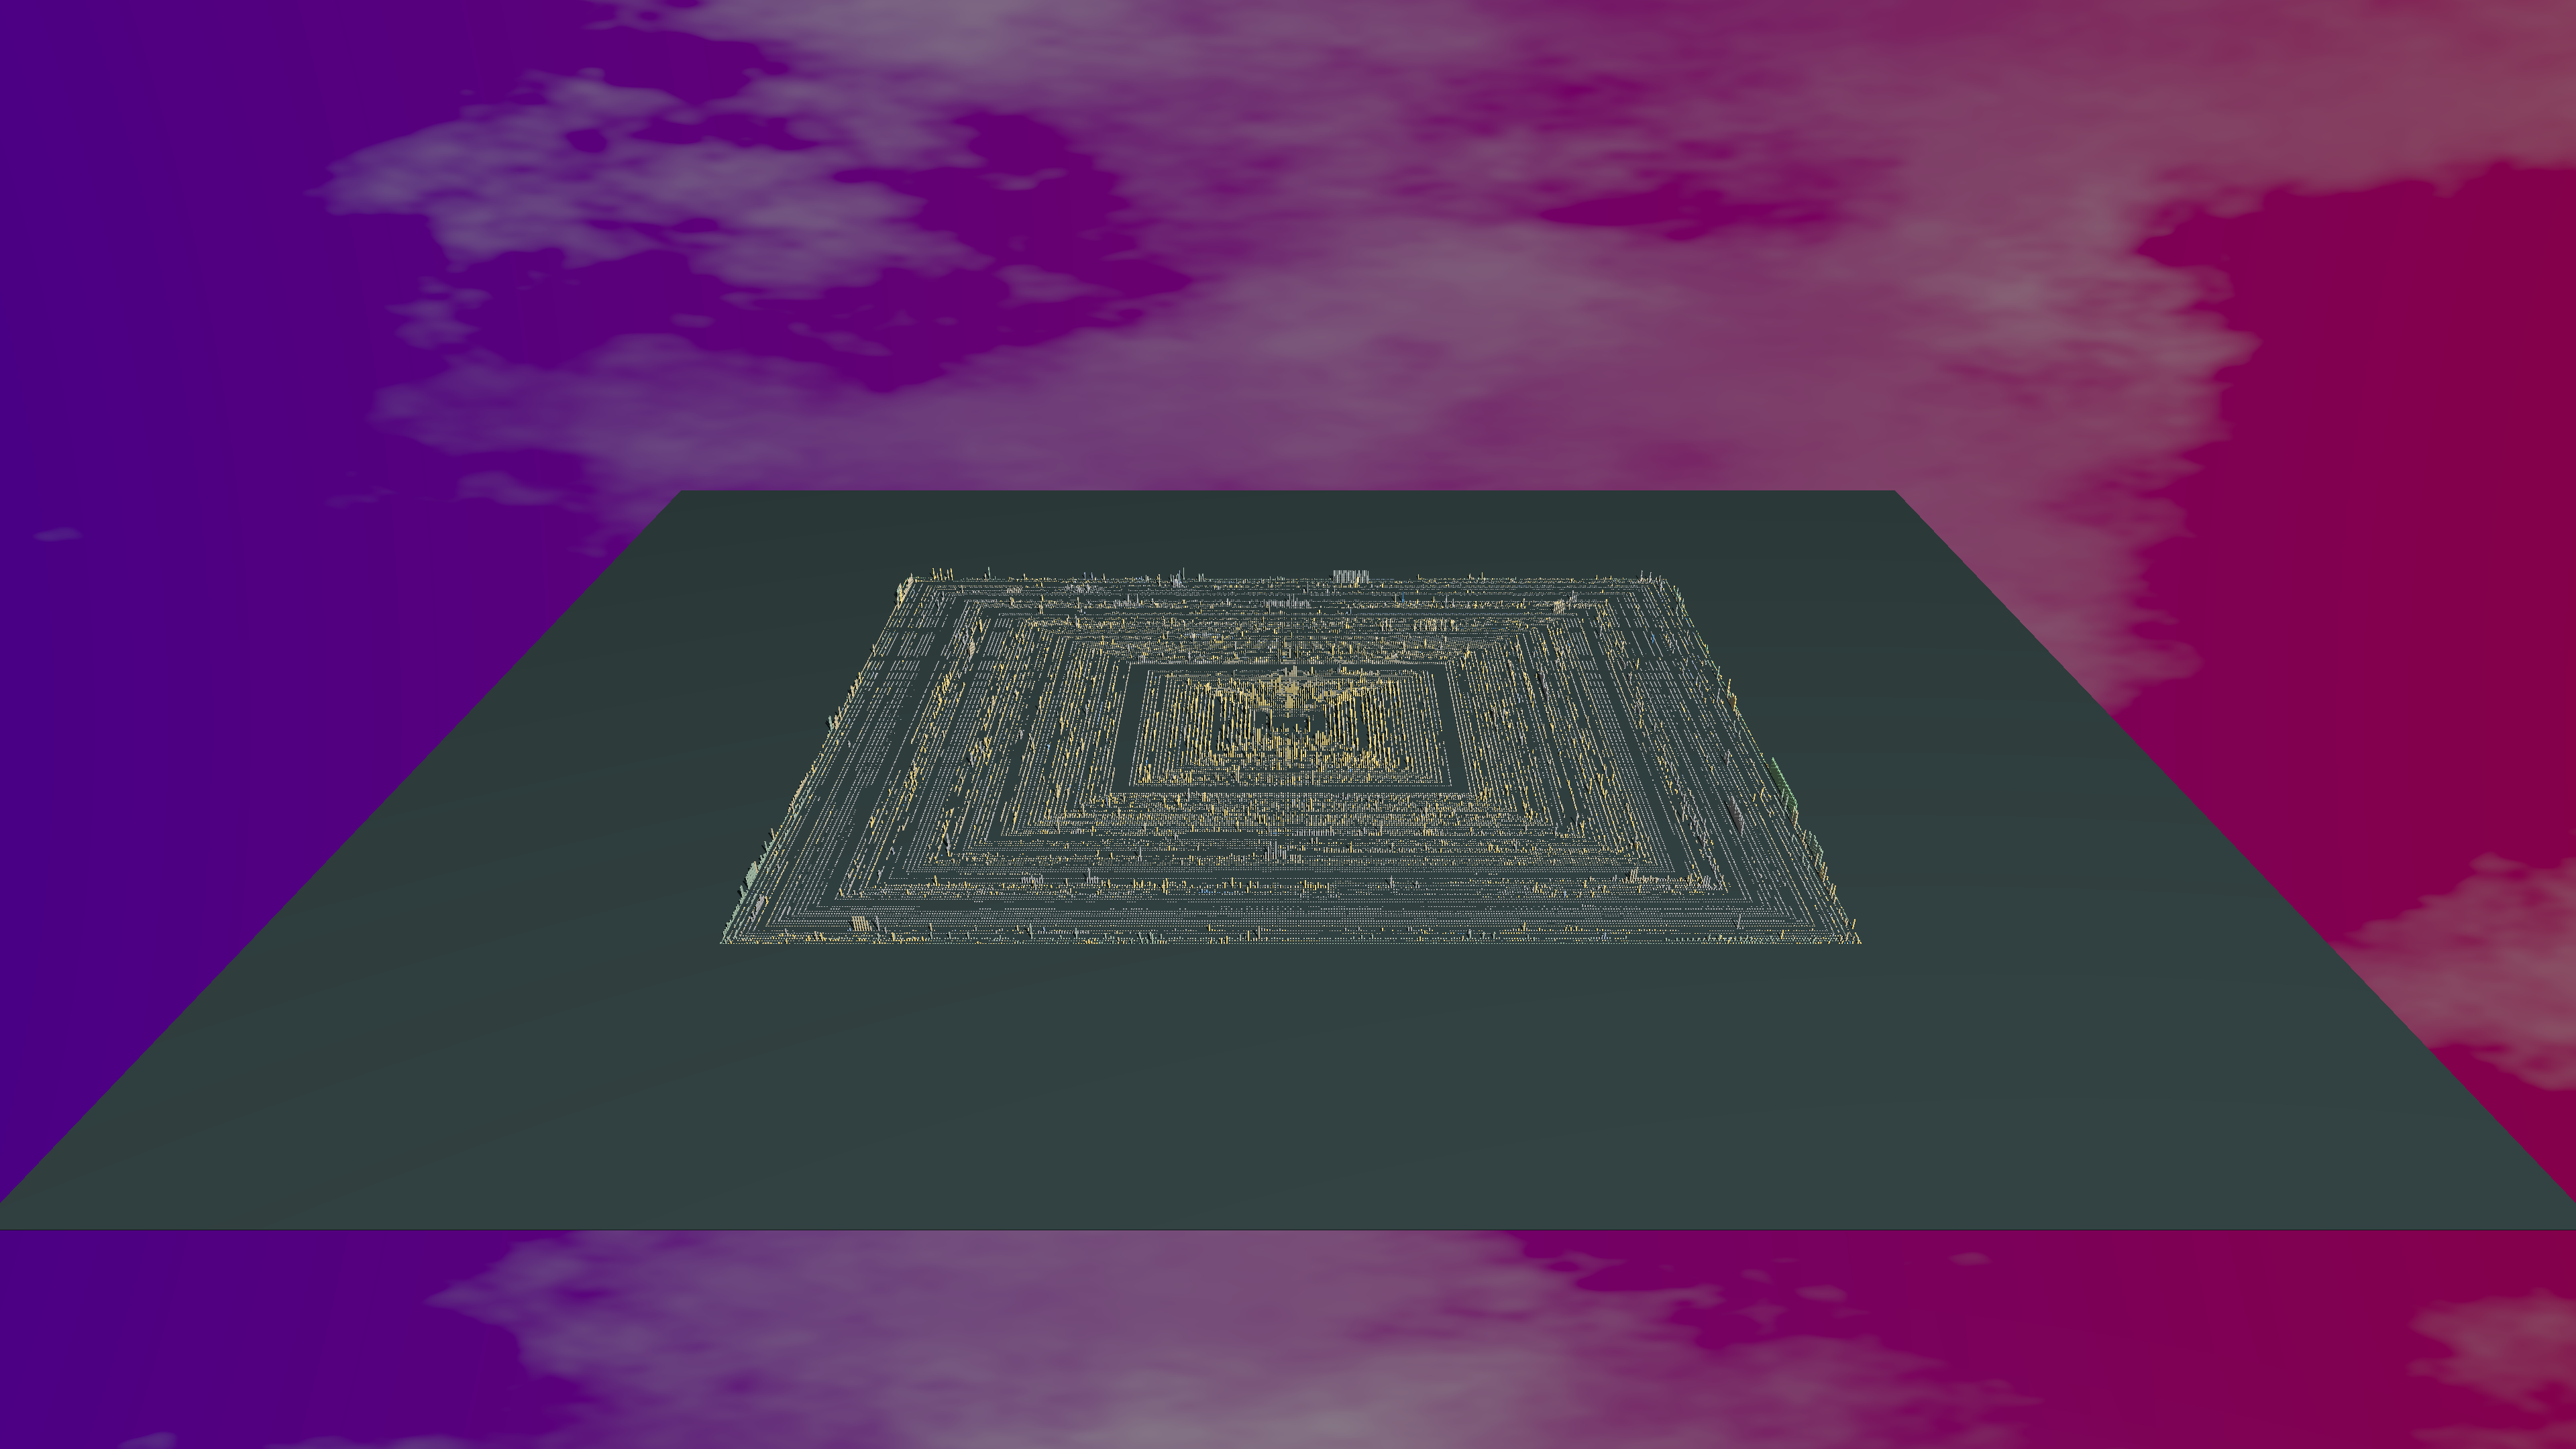
\includegraphics[width=\linewidth]{Libreoffice/Animation011.png}
        \caption{Libreoffice in March 2013 (11 year)} 
        \label{fig:Libre_V6_S4}
    \end{subfigure}
    \medskip
    \begin{subfigure}{0.48\textwidth}
        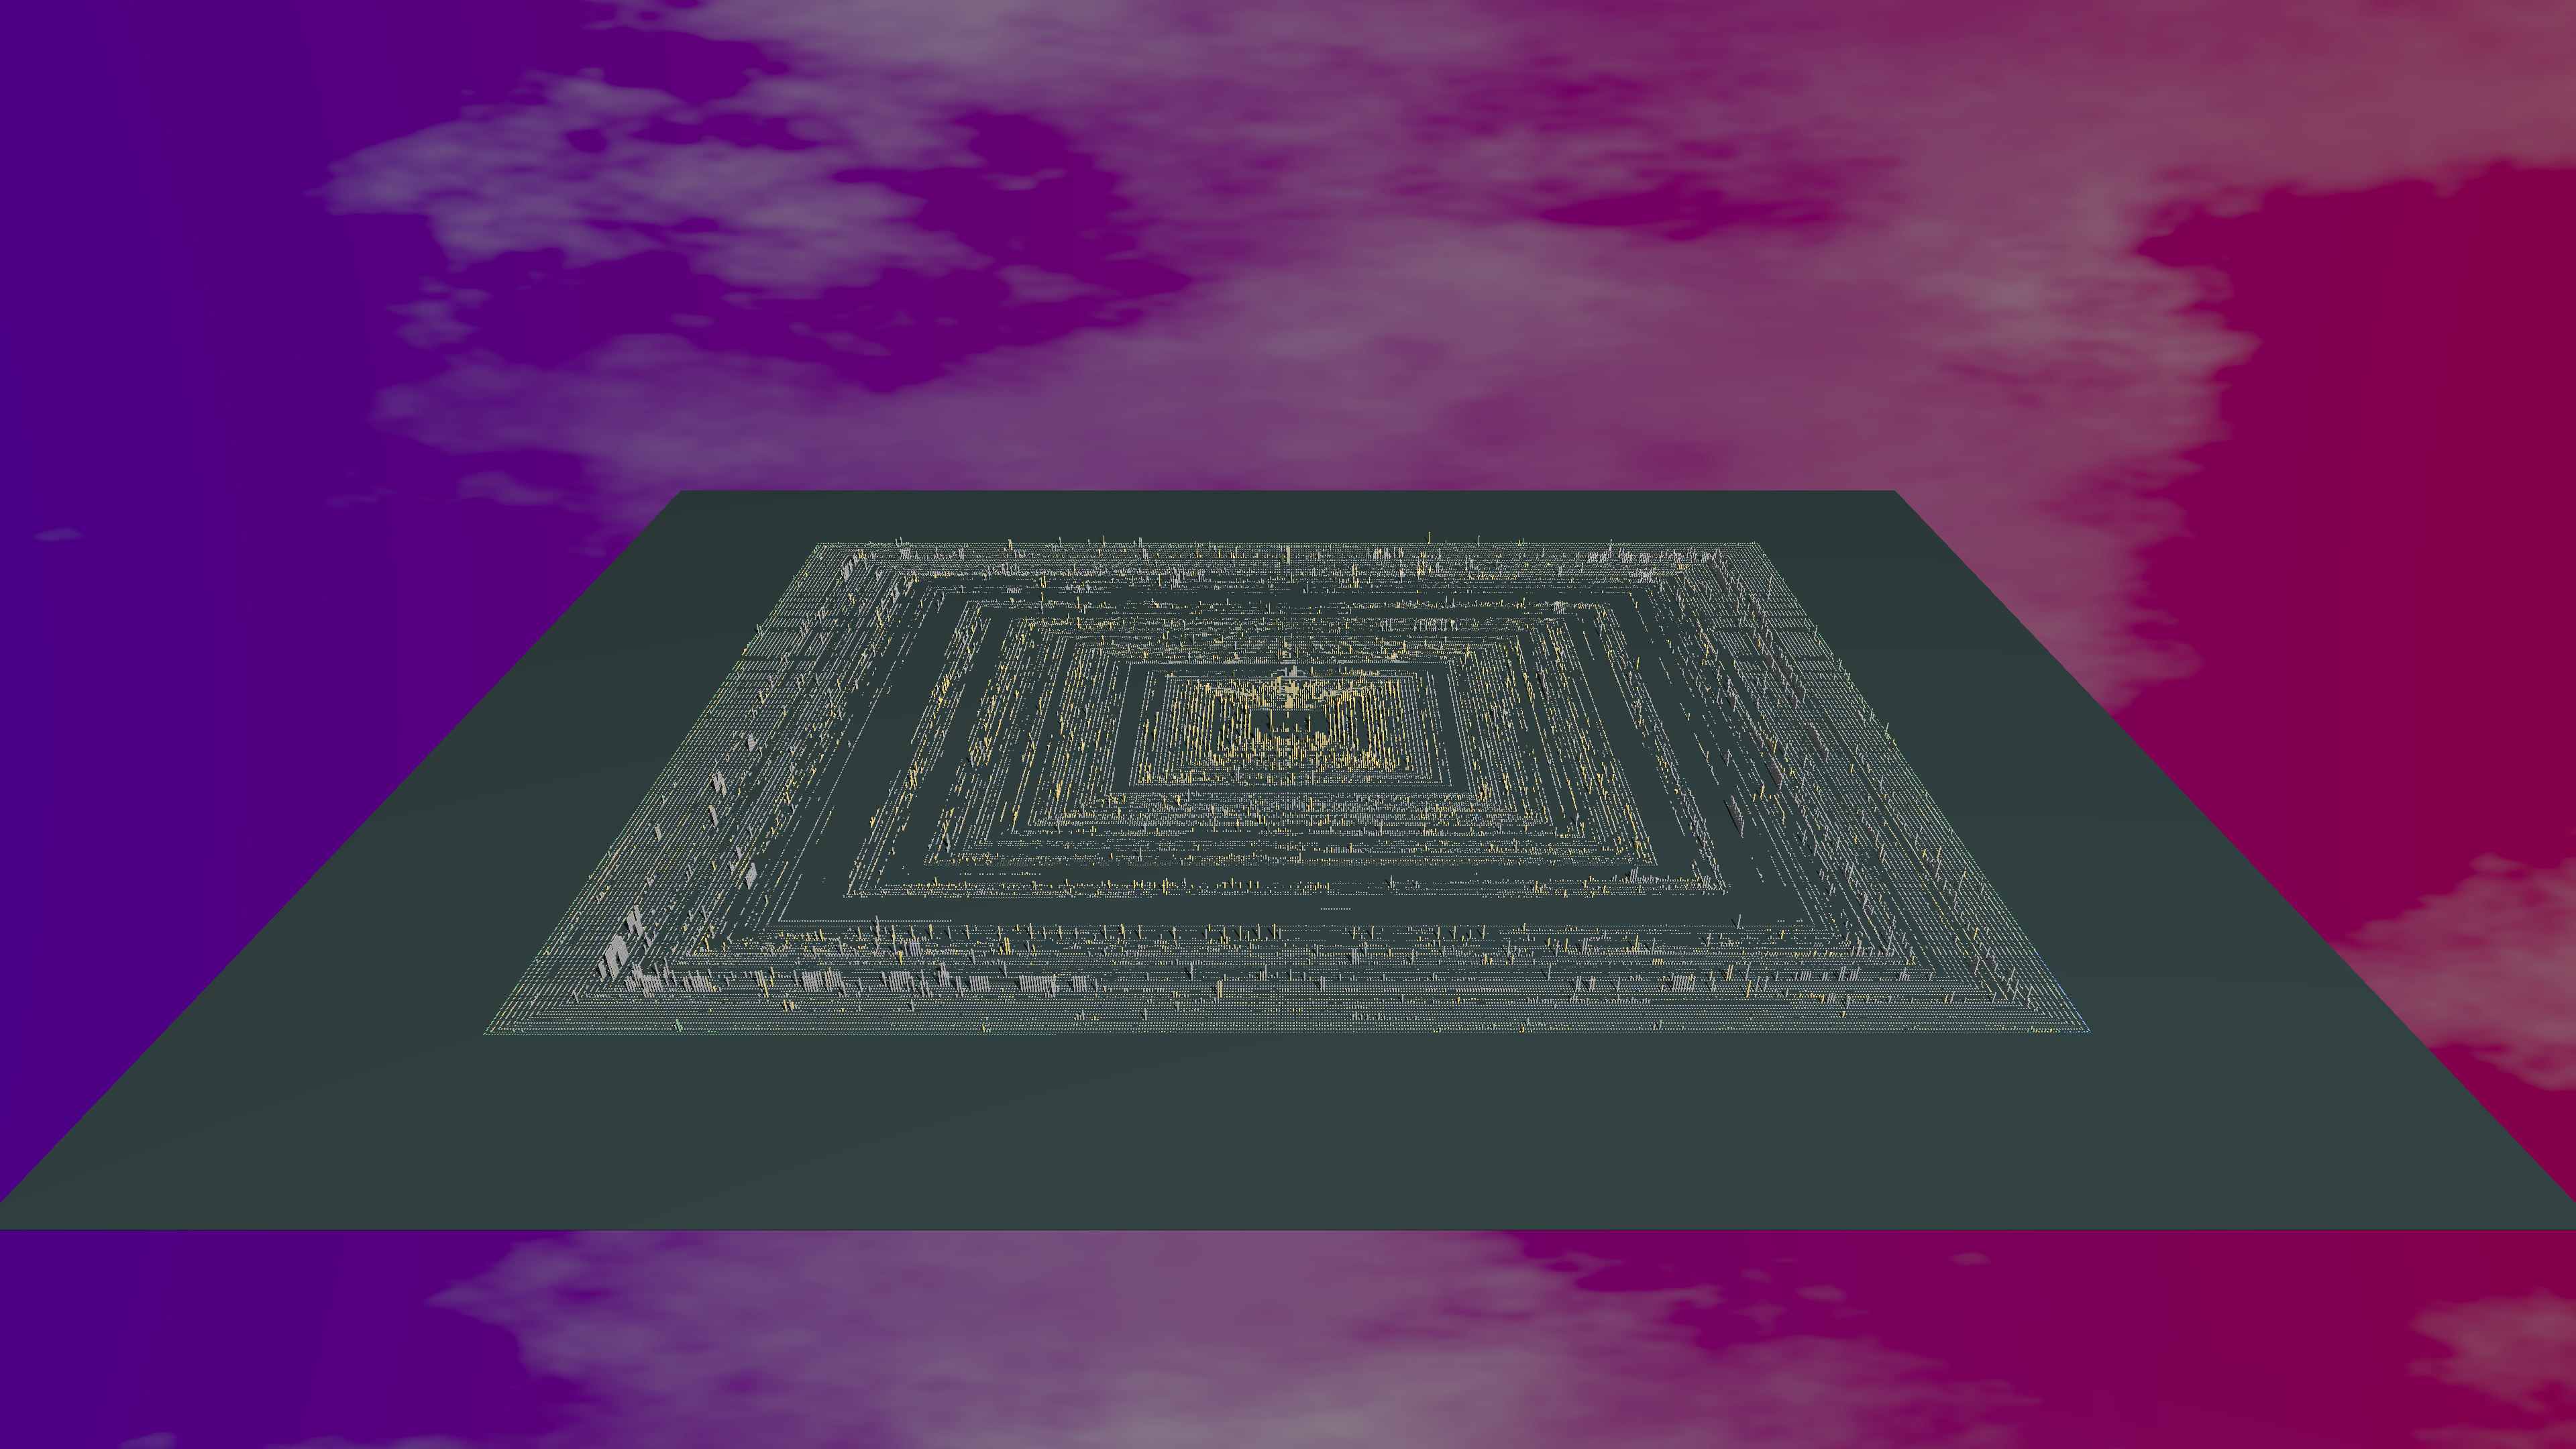
\includegraphics[width=\linewidth]{Libreoffice/Animation017.png}
        \caption{Libreoffice in March 2019 (17 year)} 
        \label{fig:Libre_V6_S5}
    \end{subfigure}\hspace*{\fill}
    \begin{subfigure}{0.48\textwidth}
        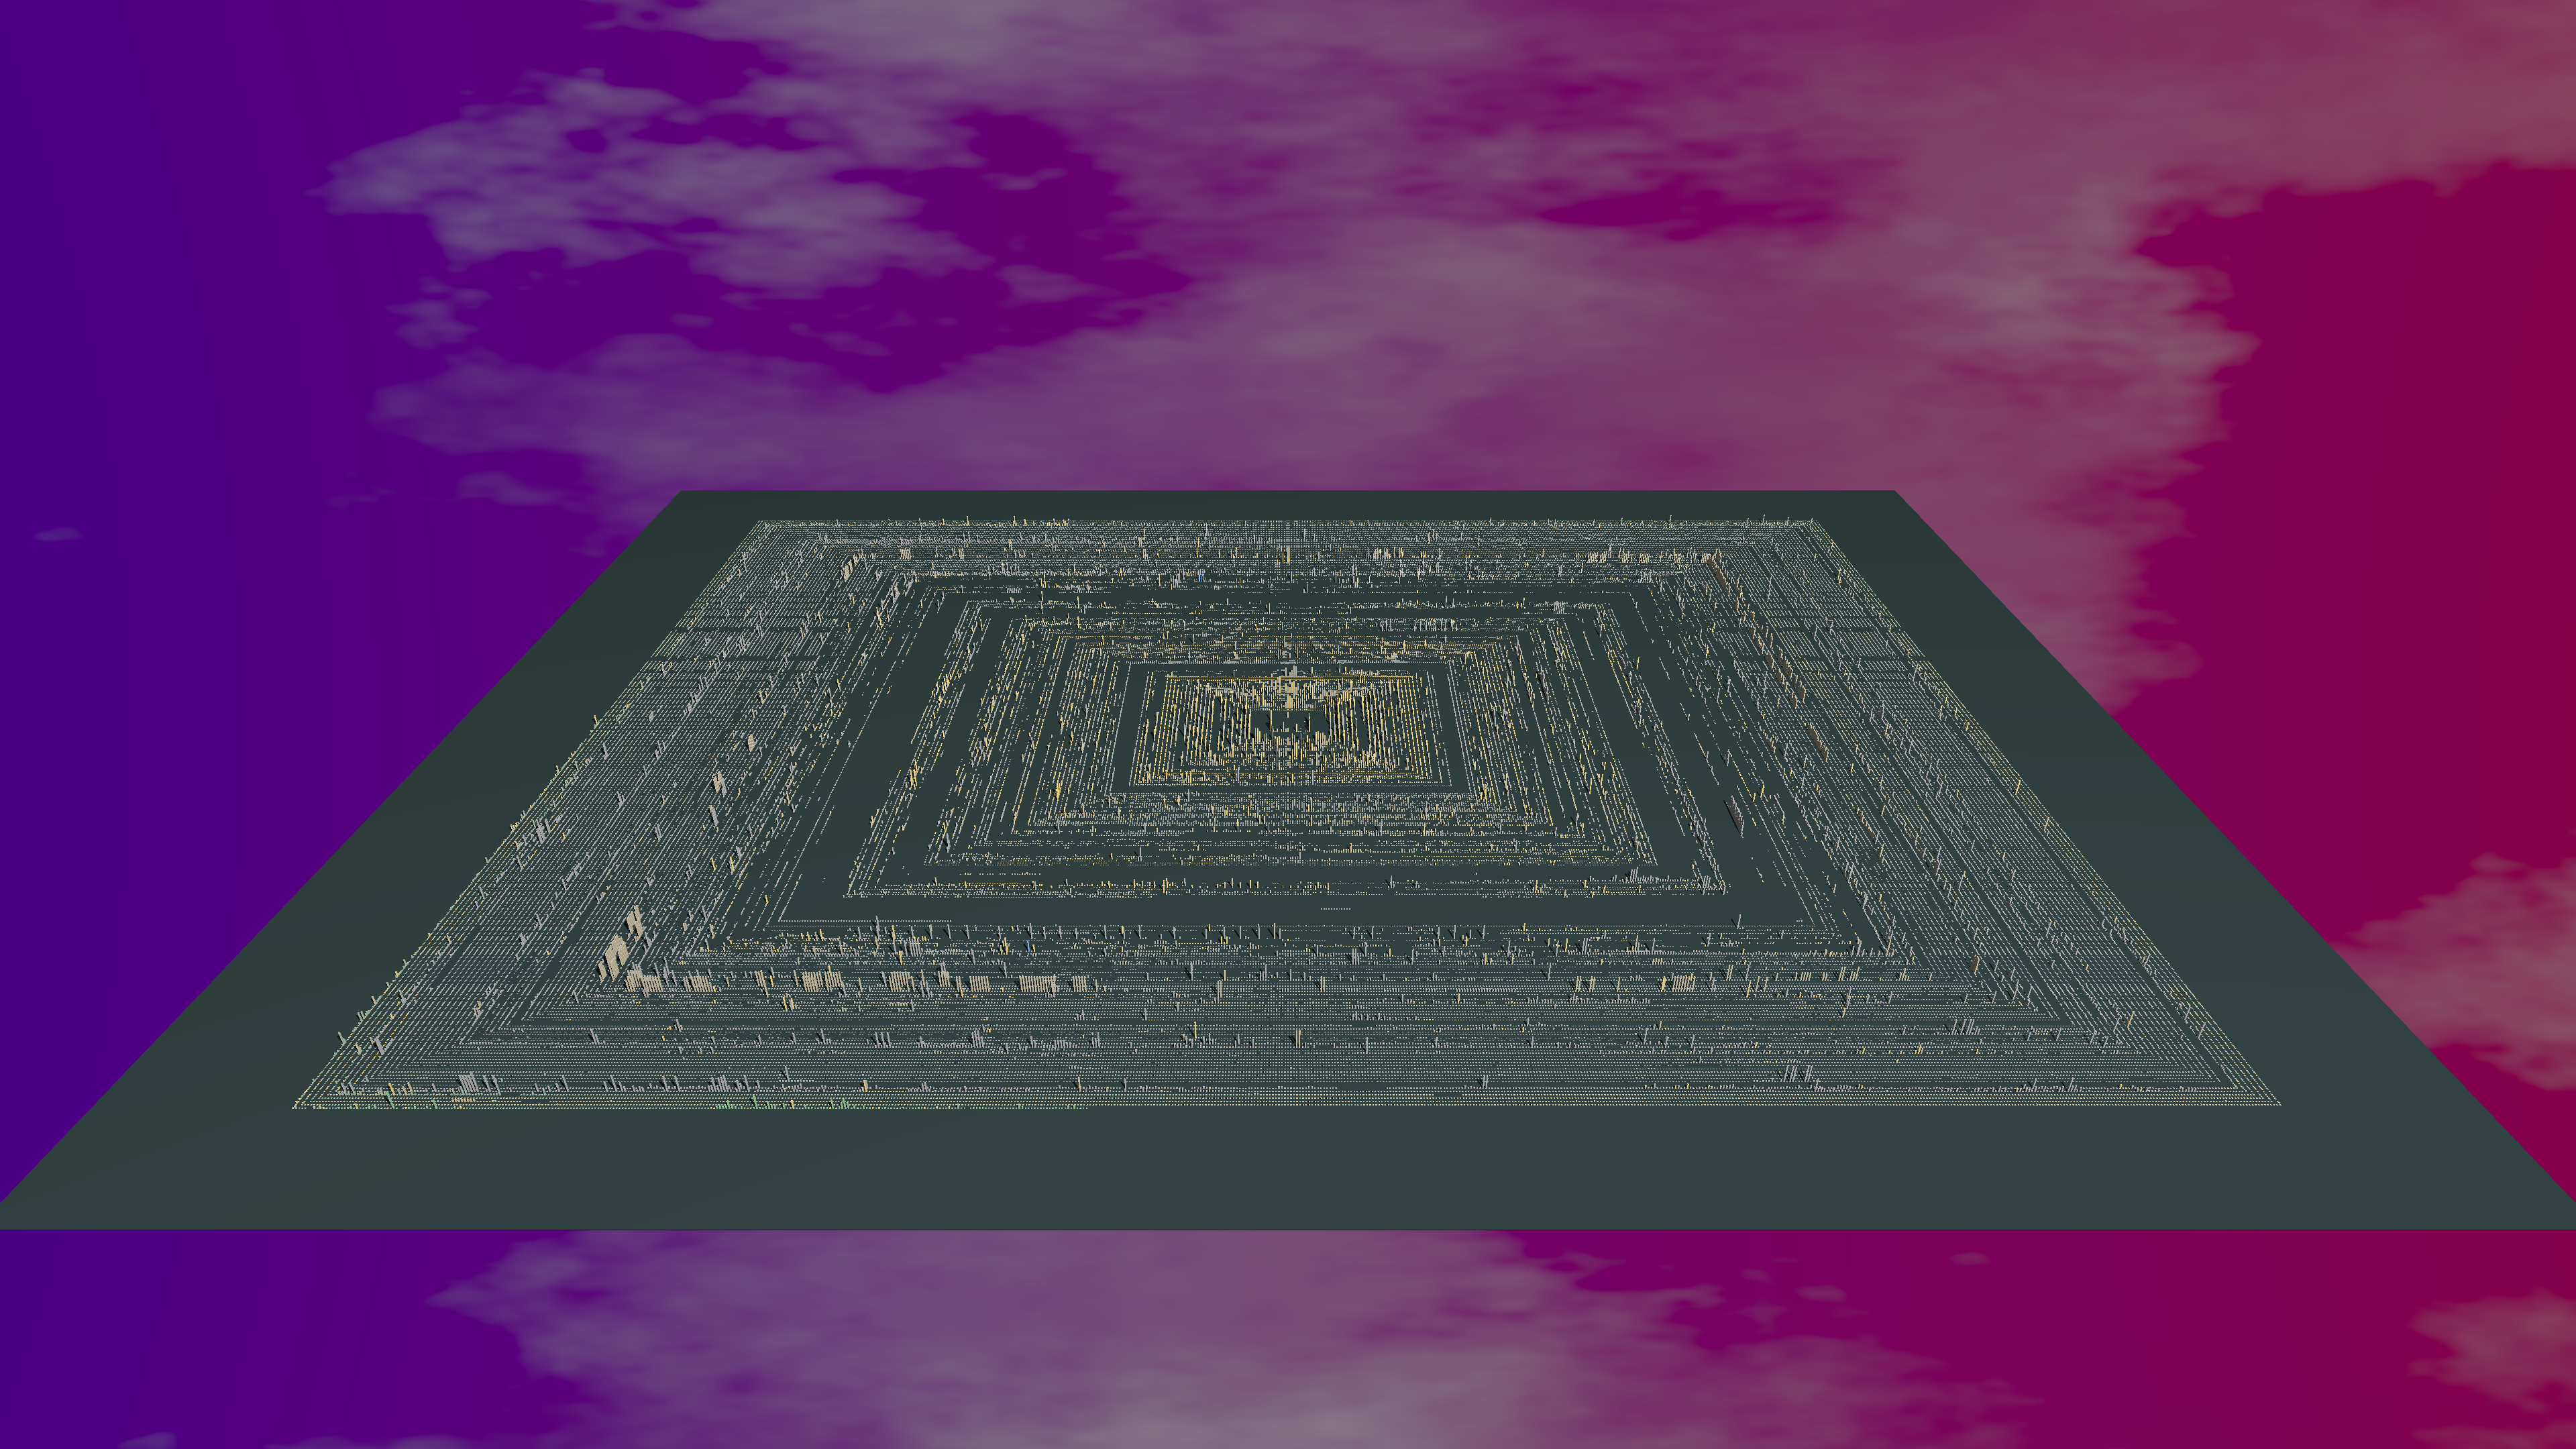
\includegraphics[width=\linewidth]{Libreoffice/Animation021.png}
        \caption{Libreoffice in June 2022 (21 year)} 
        \label{fig:Libre_V6_S6}
    \end{subfigure}
    
    \caption{Hot spots during the evolution of Libreoffice} 
    \label{fig:Libre_V6}
\end{figure}


% -------------------------------------------
% linux
% FileHistories: 109829 
% ProjectVersions: 997486 
% FileVersions: 2335535 
% First Version: 
% 	 hash: 1da177e4c3f41524e886b7f1b8a0c1fc7321cac2 
% 	 date: Sun Apr 17 00:20:36 CEST 2005 
% Last Version: 
% 	 hash: 705191b03d507744c7e097f78d583621c14988ac 
% 	 date: Tue Apr 19 19:19:02 CEST 2022 
% Diff: {DAYS=6, HOURS=18, MINUTES=58, SECONDS=26, MILLISECONDS=0, MICROSECONDS=0, NANOSECONDS=0, YEARS=17}
% -------------------------------------------
\clearpage
\section{Linux}
Everyone in the field of software engineering knows Linux. It does not need any presentation. Its code is published on GitHub, available at \url{https://github.com/torvalds/linux}. Even though its development started in 1991 by Linus Torvalds, the first commit pushed on its git repository is dated 17 April 2005. The reason is explained on the message of the first commit\footnote{\url{https://github.com/torvalds/linux/commit/1da177e4c3f41524e886b7f1b8a0c1fc7321cac2}}:
\begin{displayquote}
    Initial git repository build. I'm not bothering with the full history,
    even though we have it. We can create a separate "historical" git
    archive of that later if we want to, and in the meantime it's about
    3.2GB when imported into git - space that would just make the early
    git days unnecessarily complicated, when we don't have a lot of good
    infrastructure for it.
\end{displayquote}
He never created a repository containing the full history of Linux. The analysis on this repository detected almost 1M commits, with 109'829 FileHistories and more than 2M FileVersions. 
%\subsection{View 7}
\newline
\textbf{Goal of this visualization}
This visualization aims to see how the repository evolved through its last 17 years. We decided to adopt a commit grouping strategy based on a time window of 1 year and an aging strategy of one month with 12 steps. Hence, grey entities represent files that have not been updated for more than 12 months. 


\bigbreak
View specification adopted: same as the one defined for the View 4 (\autoref{subsec:view4}).

\textbf{Results}
Here we present only the relevant aspects of the Linux evolution we have found. However, the whole evolution is depicted in \autoref{app:Linux_Evolution}. \autoref{fig:Linux_V7} shows the hot spots during the system's evolution. \autoref{fig:Linux_V7_S1} shows the system's state in April 2006, after the first year on git. At that time, the repository had 19'709 files. For the next four years, the repository activity was active. In April 2009, as we can see from  \autoref{fig:Linux_V7_S2}, almost all the files were touched. Moreover, we can start to see a band around the core. 
After 12 years after the first commit, the system had three times its initial size. \autoref{fig:Linux_V7_S3} shows its state at that time. From this figure, we can start to notice that the spiral's center has fewer files than the edge. This is a good thing because it might mean that old files are rewritten into newer ones. Intense development activity on Linux continued uninterruptedly until April 2022. As we can see from \autoref{fig:Linux_V7_S4}, \autoref{fig:Linux_V7_S5} and \autoref{fig:Linux_V7_S6} during its recent growing process, the center slowly became rarefied. This is a sign that older files are now rewritten into newer ones. 
\bigbreak
\textbf{Conclusion}
 We saw how the codebase of Linux evolved since their move to git. The development activity was constant throughout these 17 years. The codebase started with 19'705 files and reached 77'183 in April 2022, almost four times its original size. During this time, they evolved the kernel to develop new features and started a sort of modern process to slowly get rid of the files that were added 17 years ago. As we can see, the center of the spiral started to become rarefied. Nonetheless, it still holds many files, which means that the current version of Linux relies on files written more than 17 years ago. 
\bigbreak
\textbf{Video}
We packed in a video the visualization that we presented with auditive support. The video is available at \url{https://workInProgress.com}


\begin{figure}[ht]
    \begin{subfigure}{0.48\textwidth}
        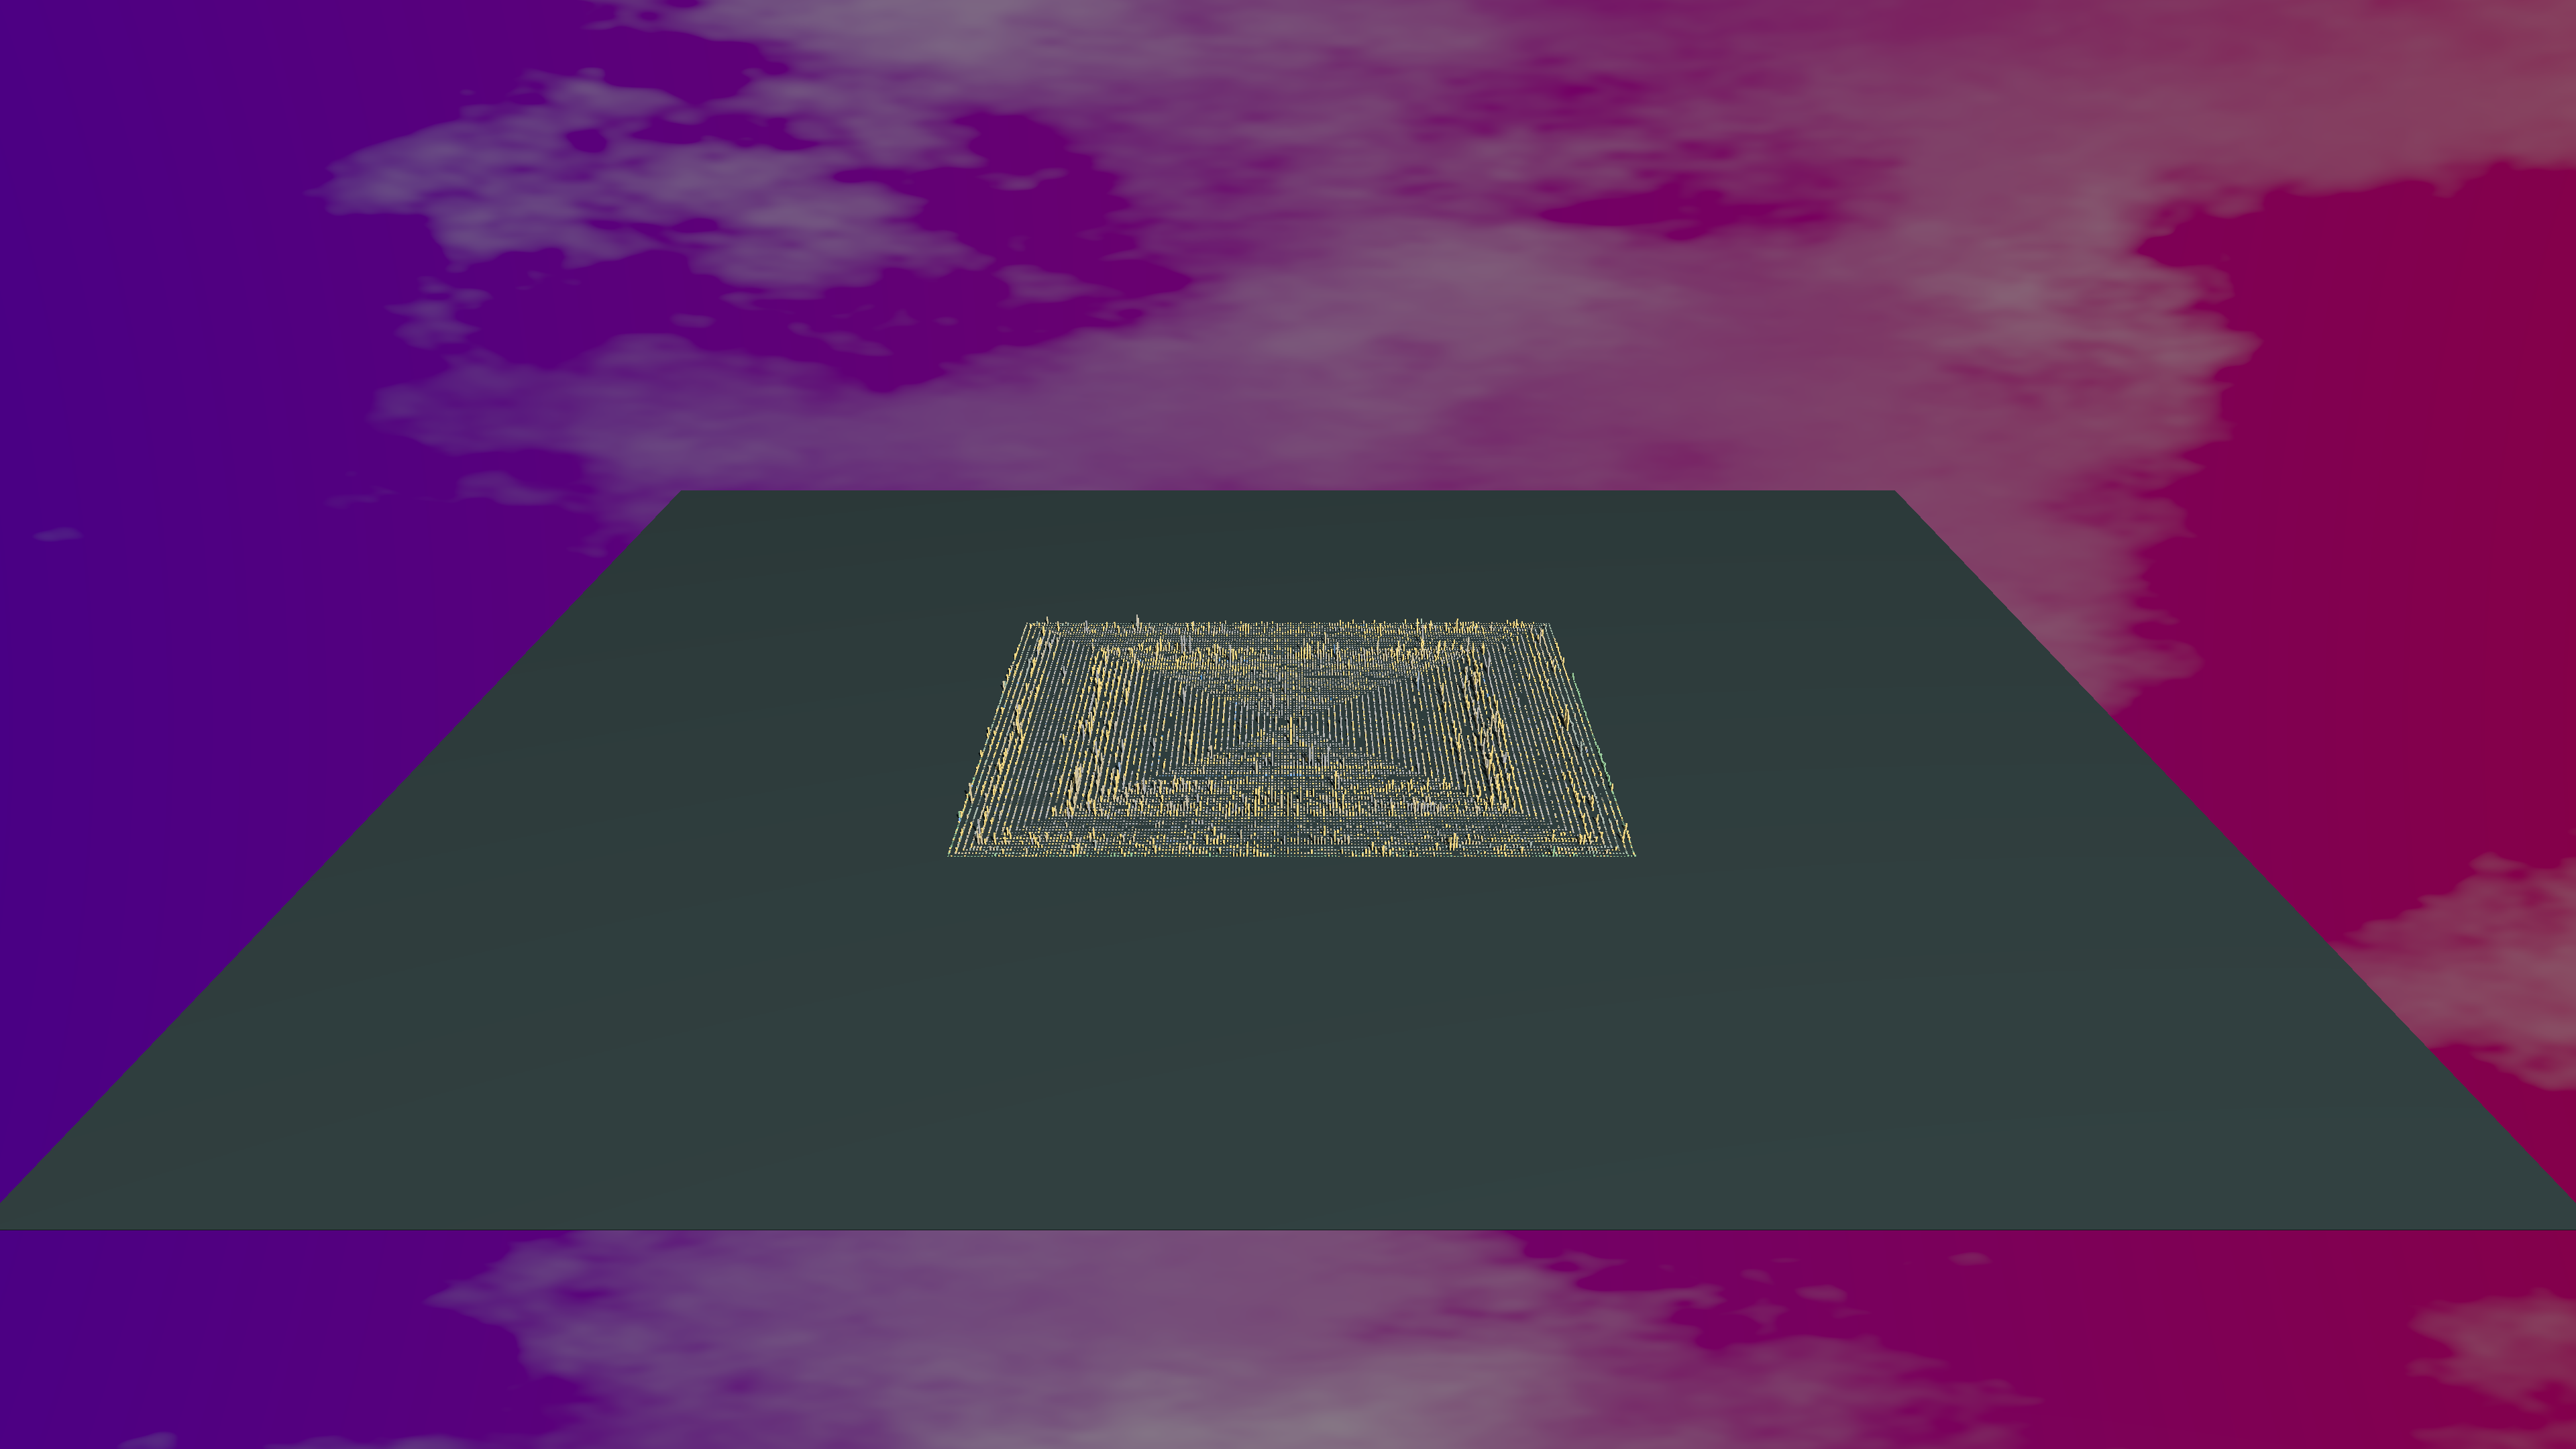
\includegraphics[width=\linewidth]{Linux/Animation001.png}
        \caption{Linux in April 2006 (1 year)} 
        \label{fig:Linux_V7_S1}
    \end{subfigure}\hspace*{\fill}
    \begin{subfigure}{0.48\textwidth}
        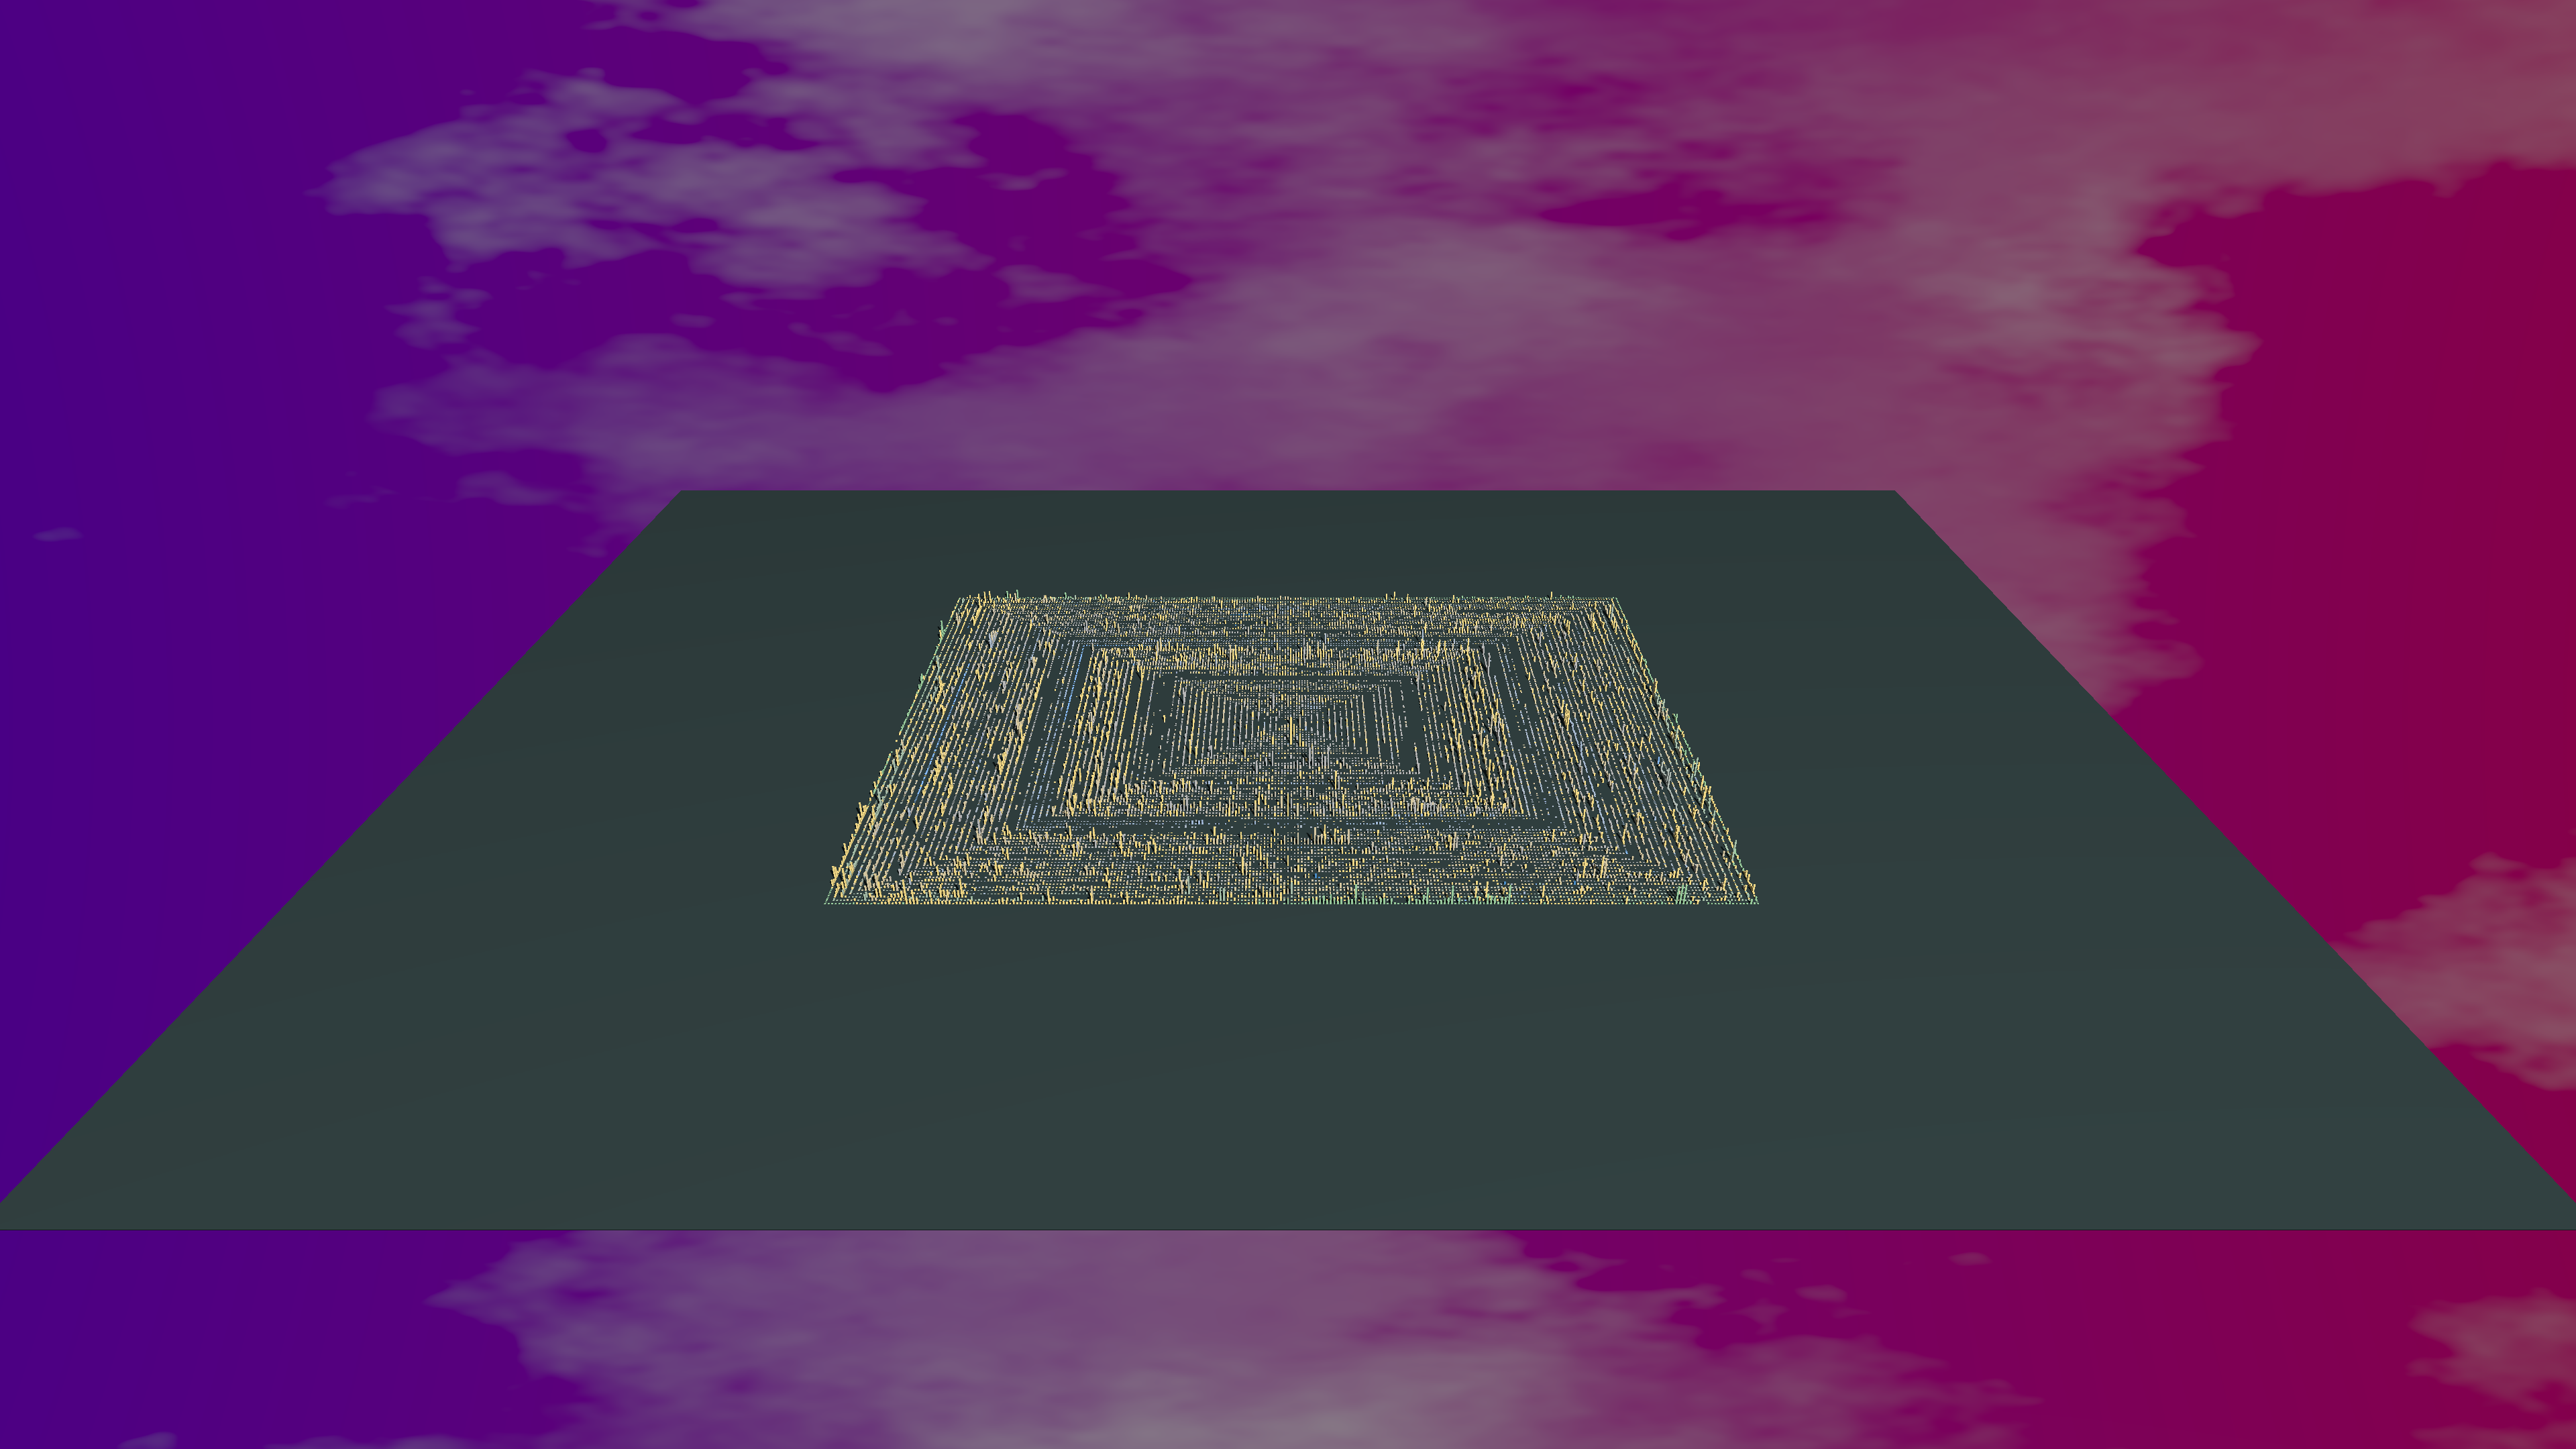
\includegraphics[width=\linewidth]{Linux/Animation004.png}
        \caption{Linux in April 2009 (4 year)} 
        \label{fig:Linux_V7_S2}
    \end{subfigure}
    \medskip
    \begin{subfigure}{0.48\textwidth}
        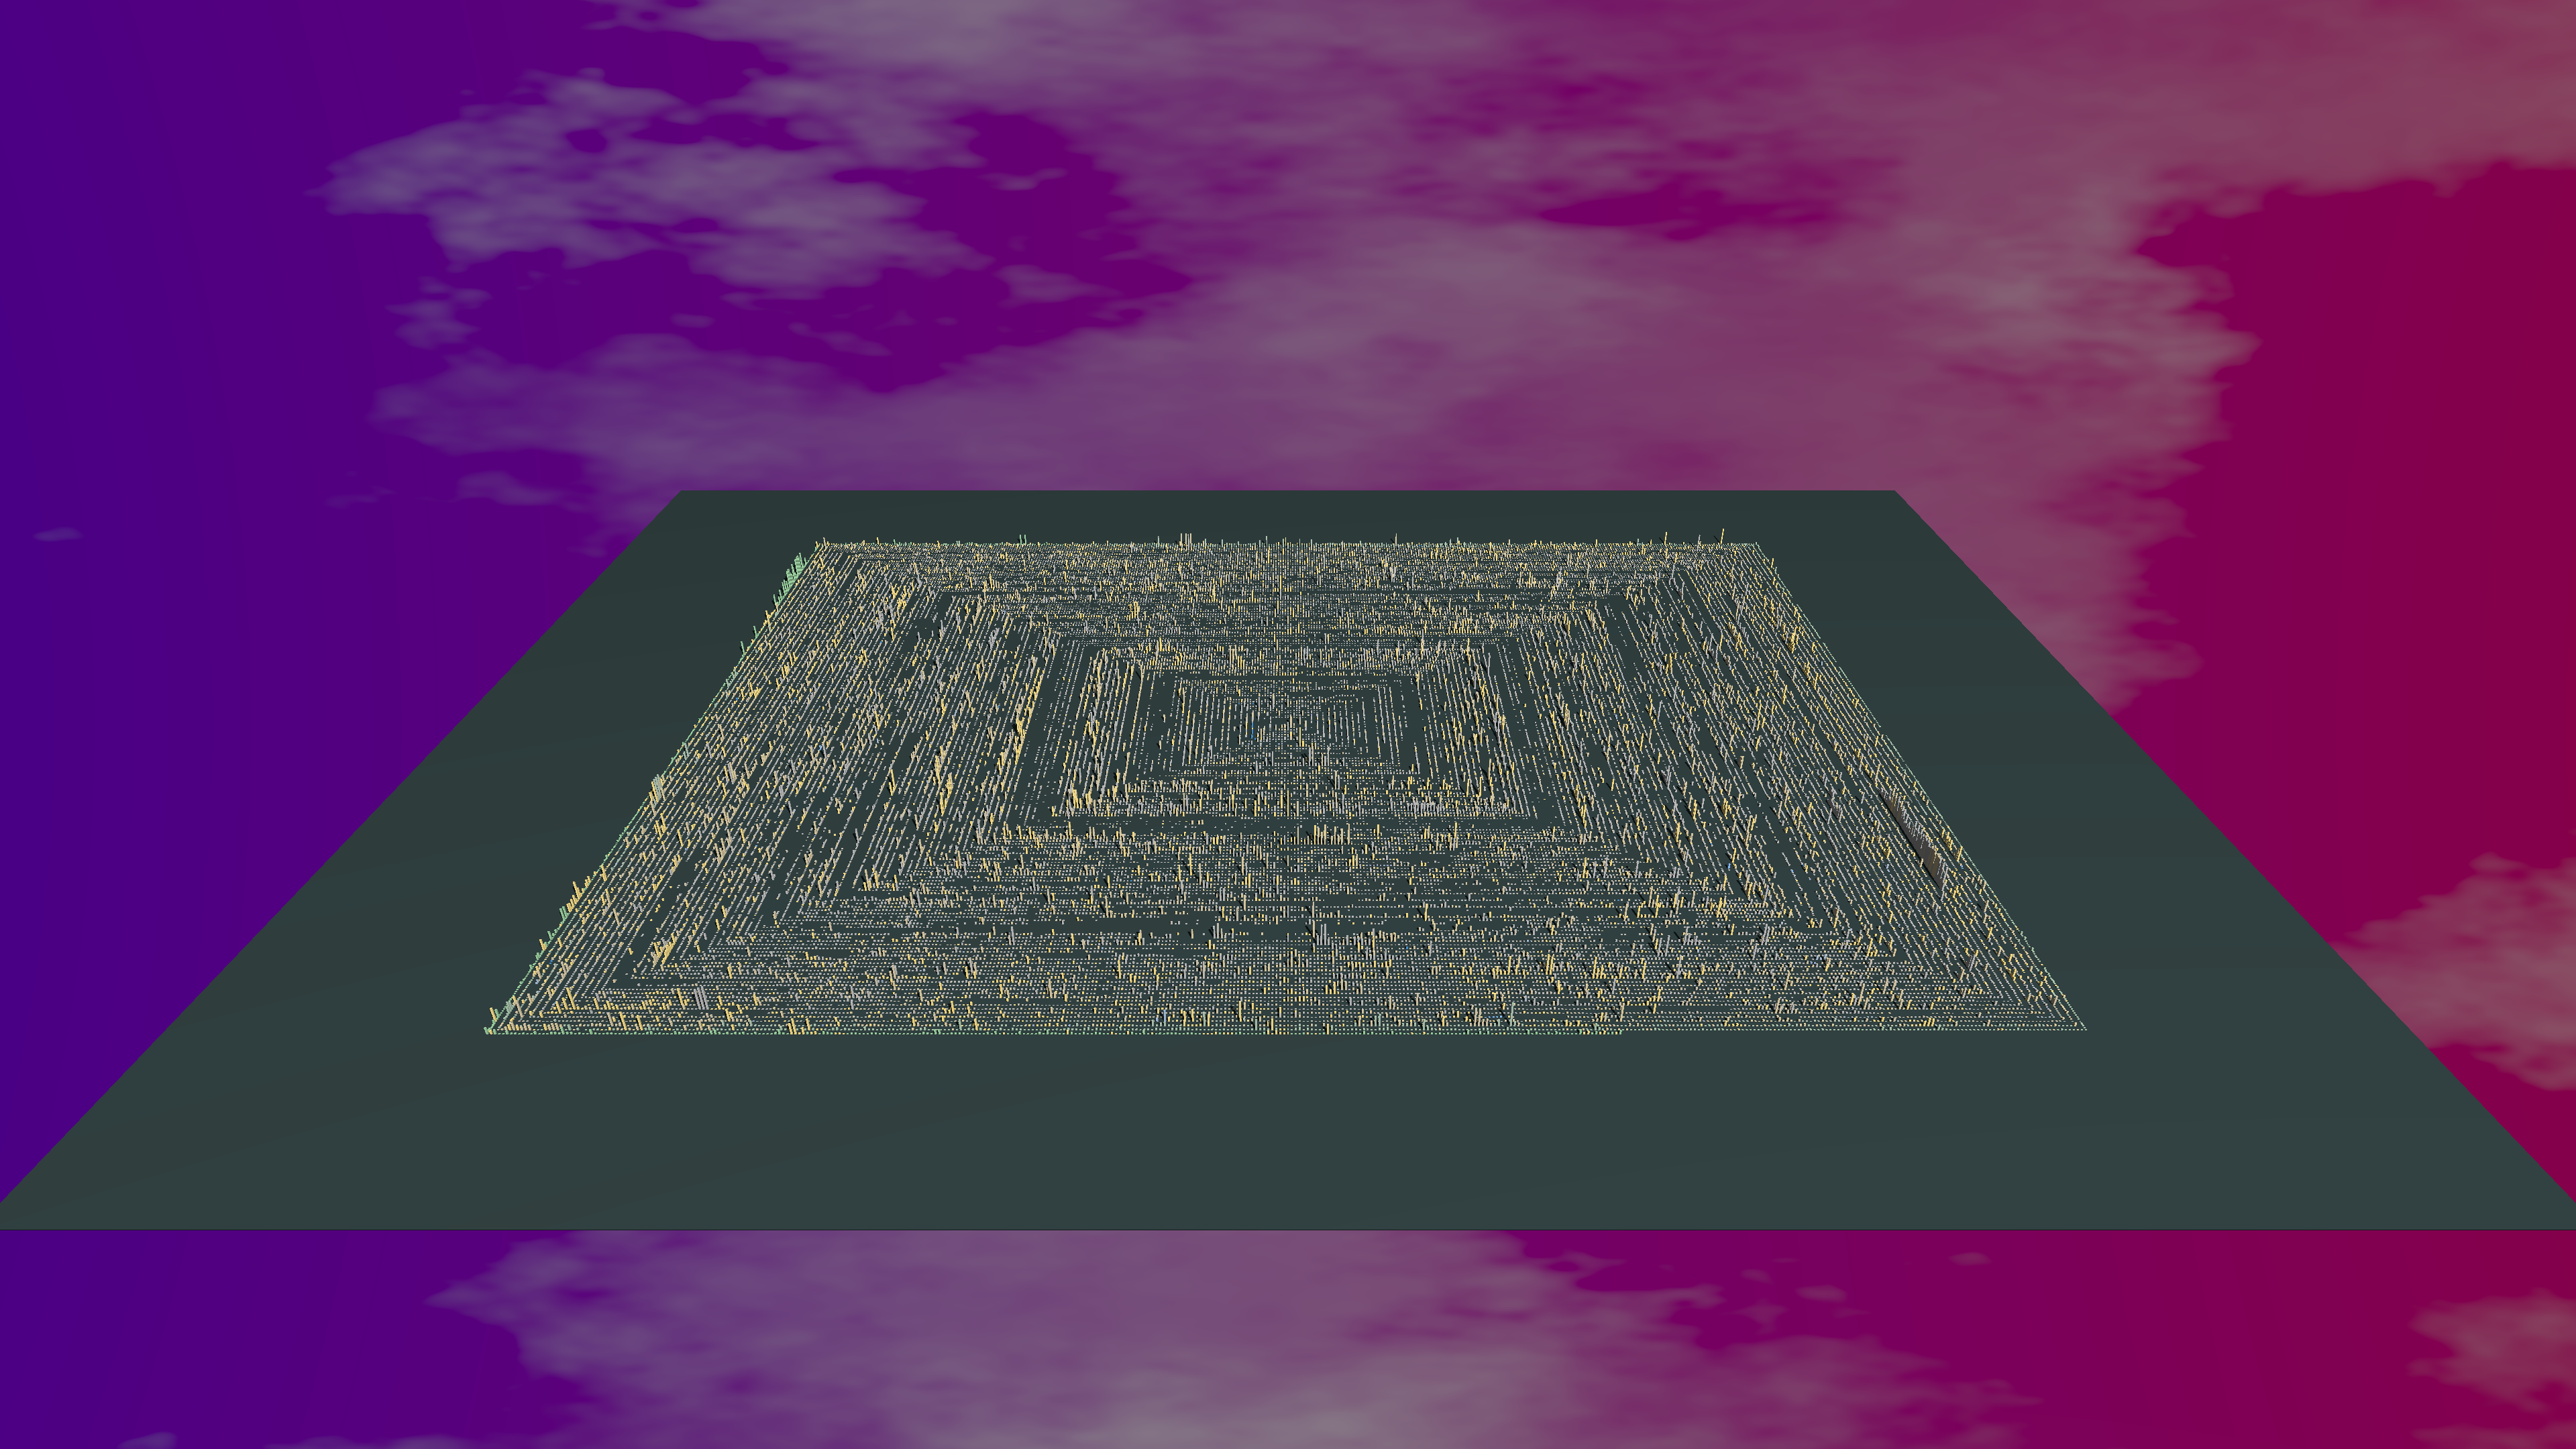
\includegraphics[width=\linewidth]{Linux/Animation012.png}
        \caption{Linux in April 2017 (12 year)} 
        \label{fig:Linux_V7_S3}
    \end{subfigure}\hspace*{\fill}
    \begin{subfigure}{0.48\textwidth}
        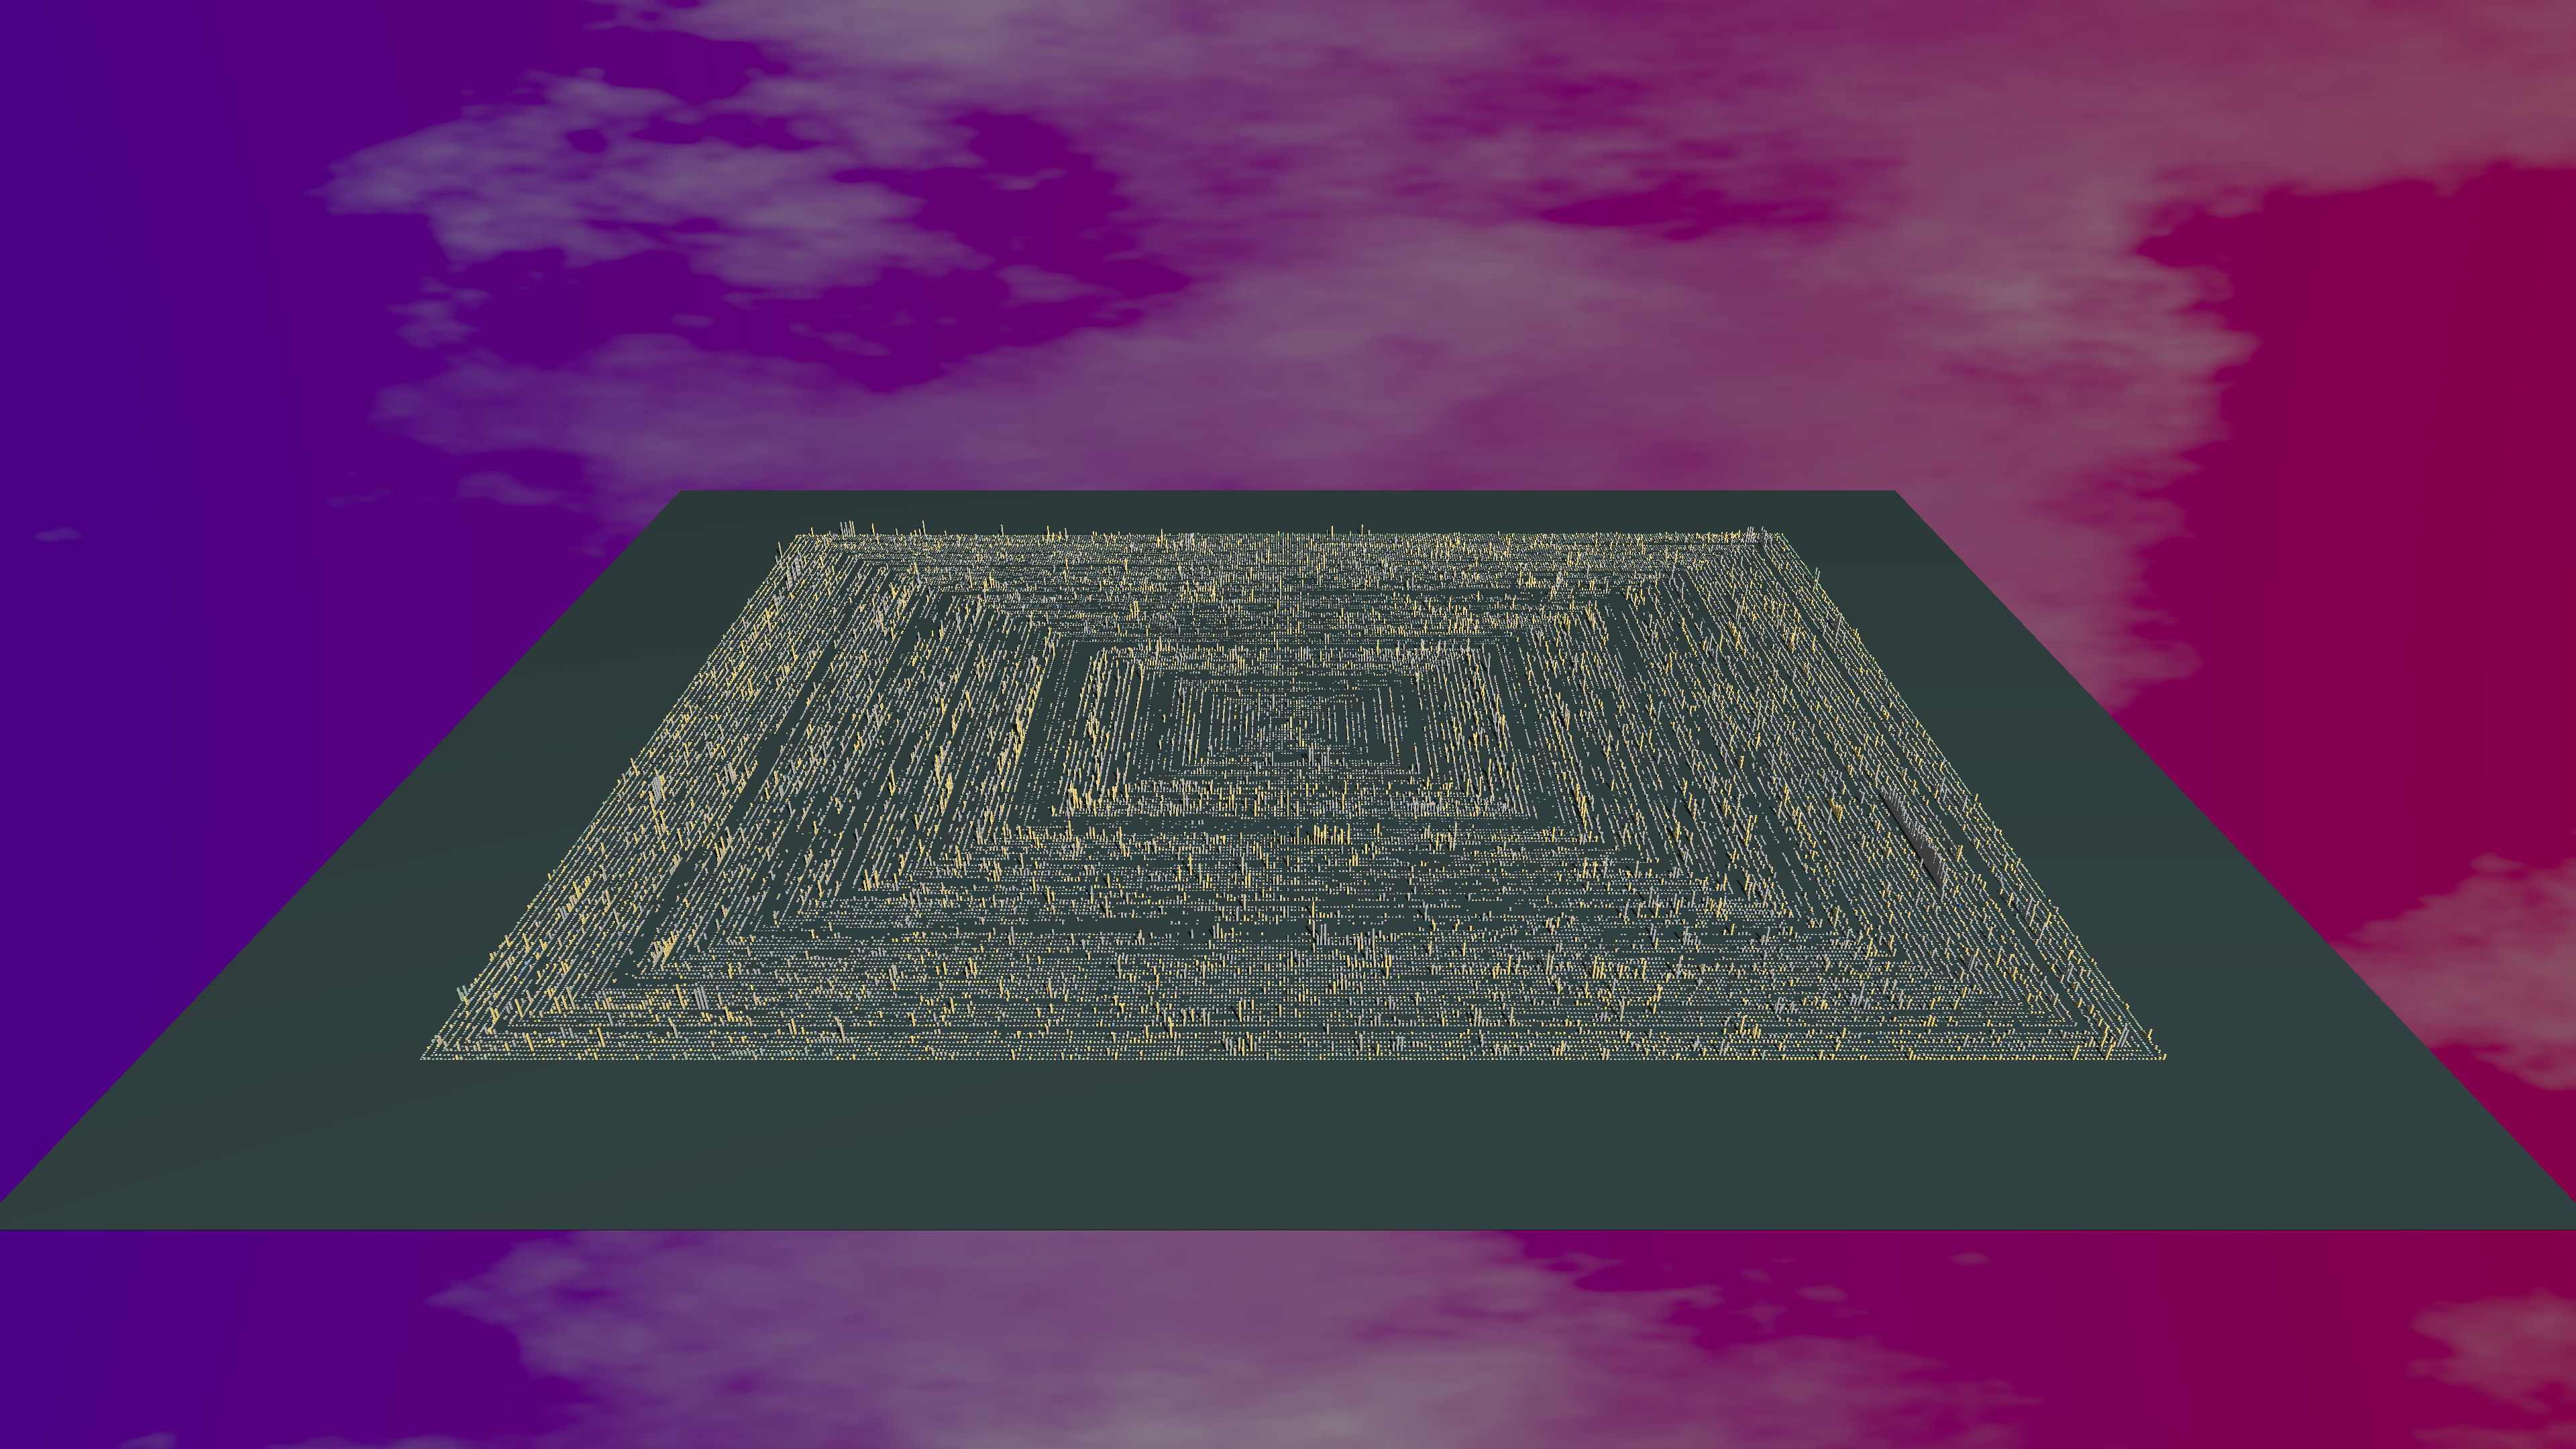
\includegraphics[width=\linewidth]{Linux/Animation014.png}
        \caption{Linux in April 2019  (14 year)} 
        \label{fig:Linux_V7_S4}
    \end{subfigure}
    \medskip
    \begin{subfigure}{0.48\textwidth}
        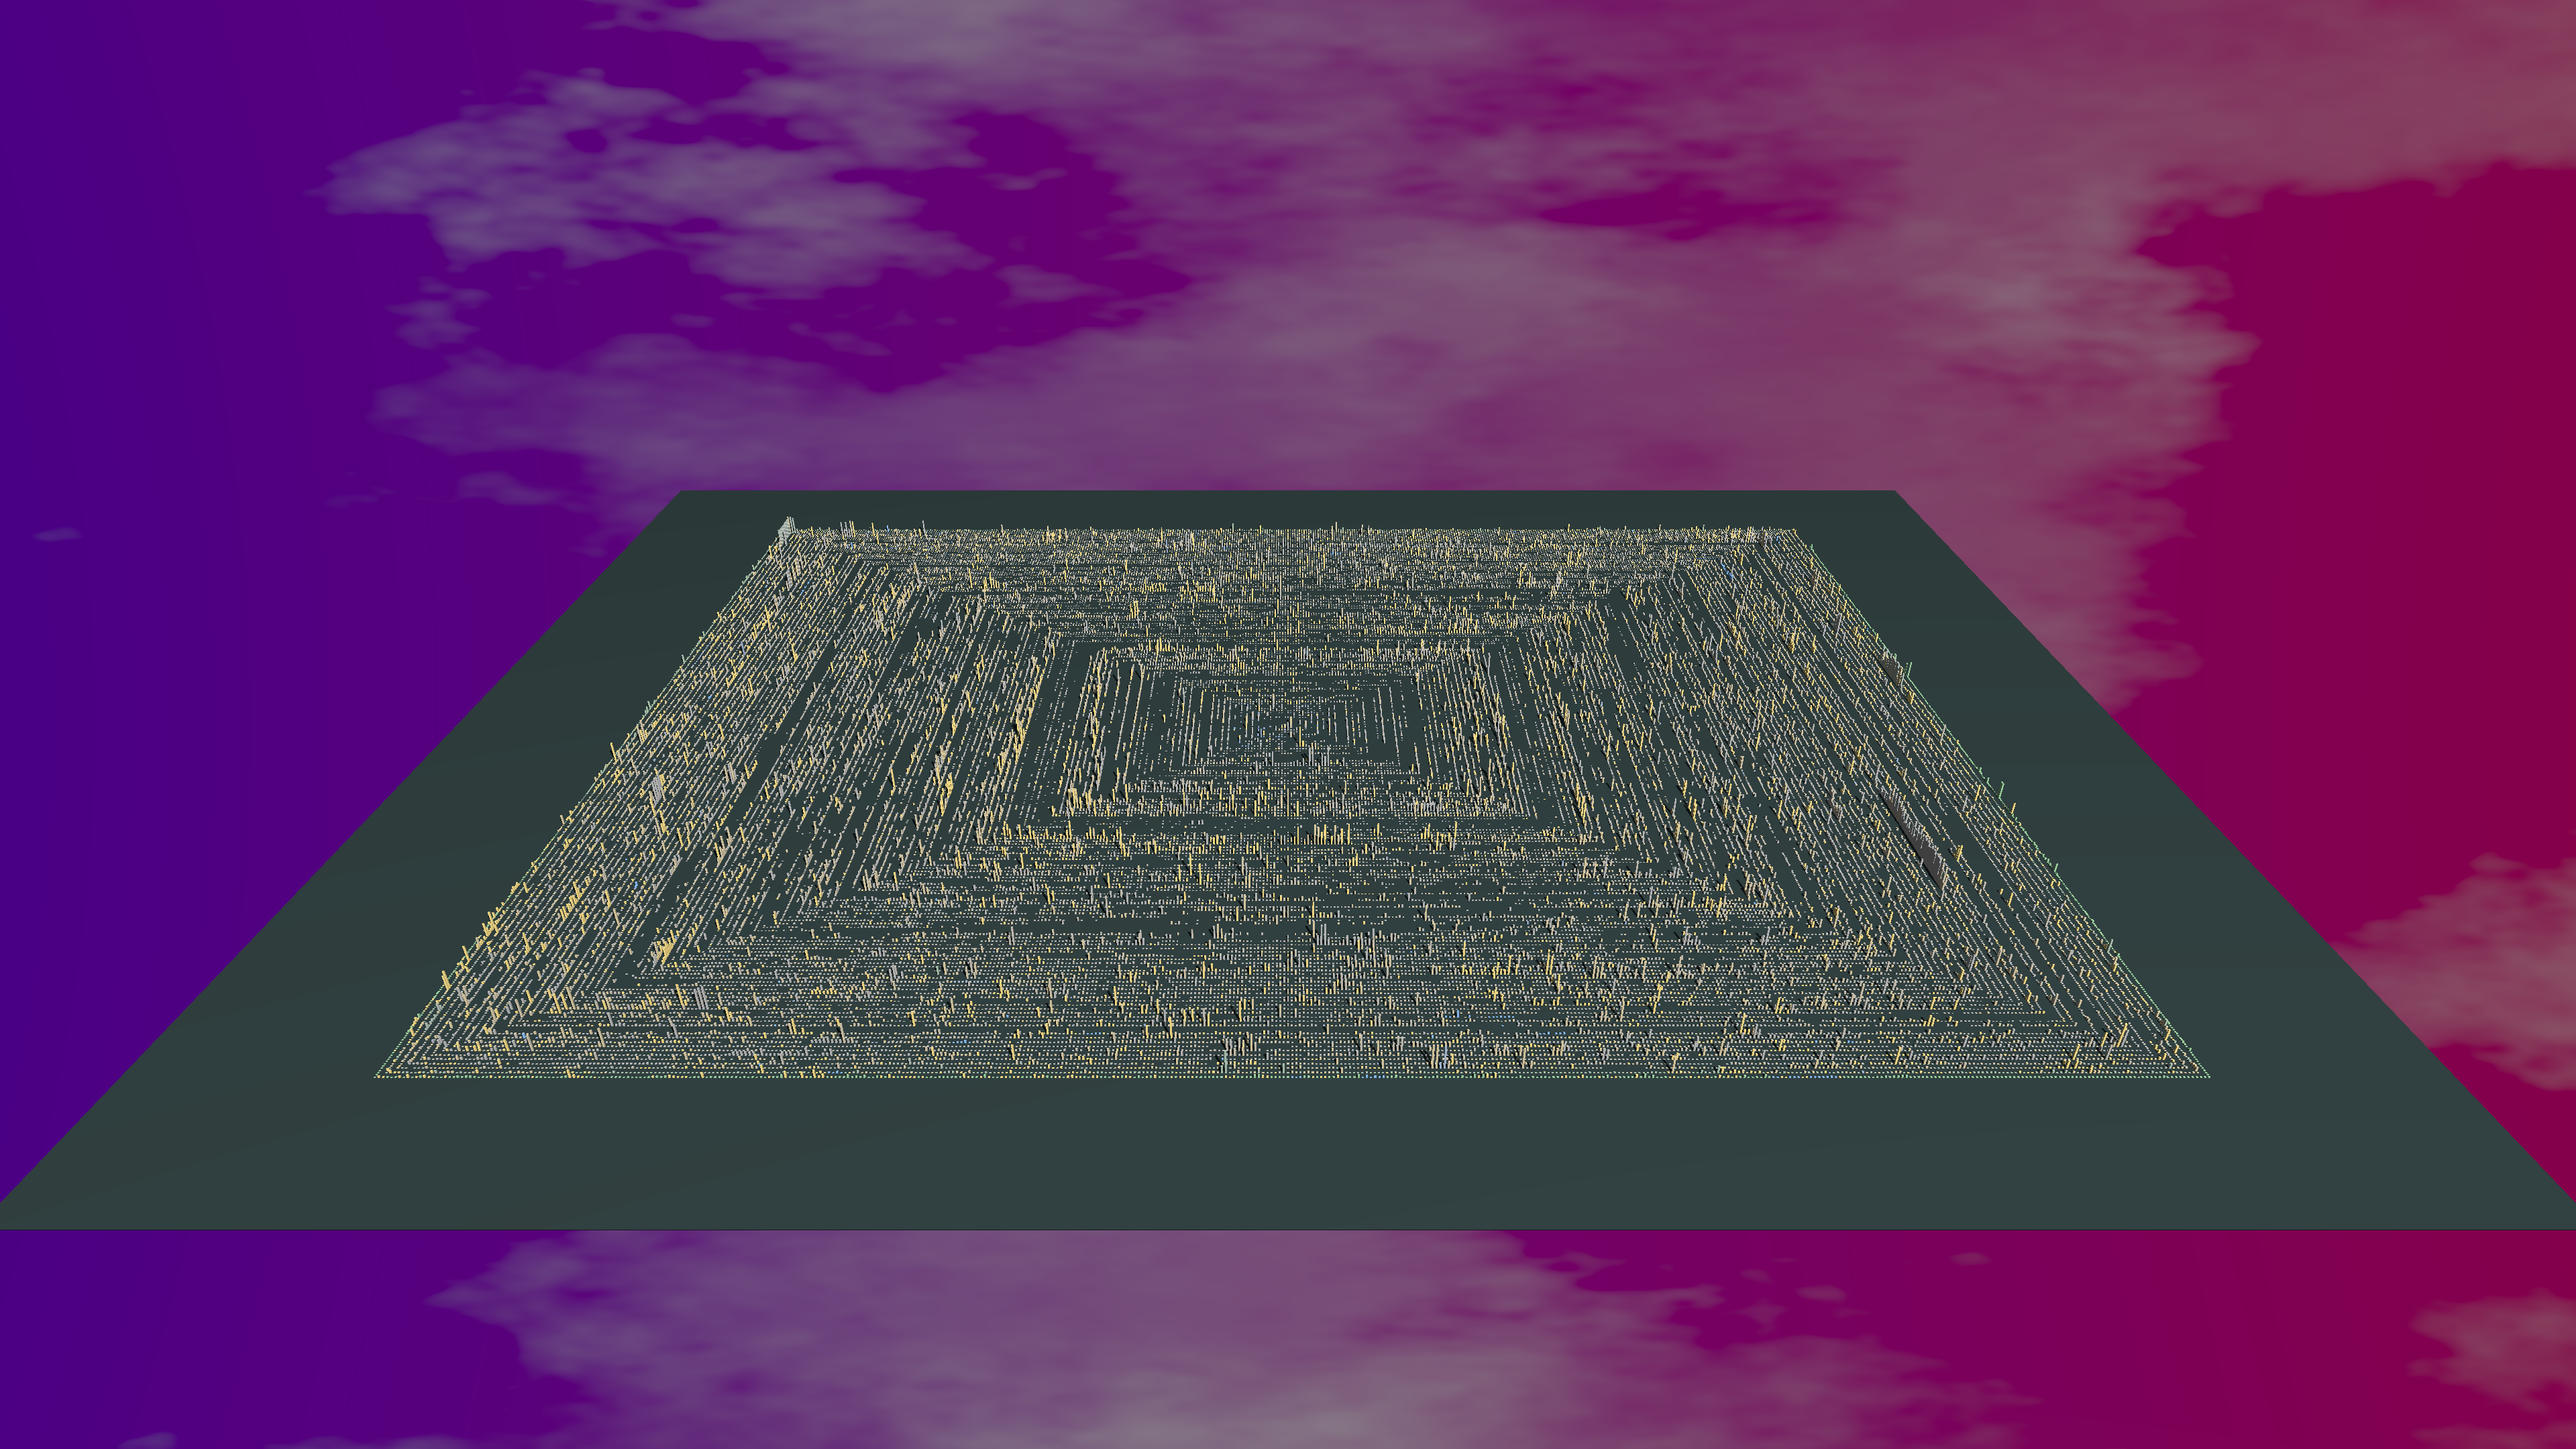
\includegraphics[width=\linewidth]{Linux/Animation015.png}
        \caption{Linux in April 2020 (15 year)} 
        \label{fig:Linux_V7_S5}
    \end{subfigure}\hspace*{\fill}
    \begin{subfigure}{0.48\textwidth}
        \includegraphics[width=\linewidth]{Linux/Animation017.png}
        \caption{Linux in April 2022 (17 year)} 
        \label{fig:Linux_V7_S6}
    \end{subfigure}
    
    \caption{Hot spots during the evolution of Linux} 
    \label{fig:Linux_V7}
\end{figure}

\clearpage
To give to the reader an idea about the size of those systems, we took the last AnimationFrame of each project analyzed and we put them in \autoref{fig:SizeComparison}. Even though Linux was initially bigger than Libreoffice, the latter grew sharply in the last year, overtaking the biggest repository on GitHub. Furthermore, from this picture, we can appreciate the different development paths that each system took. For example, ArgoUML is the only repository that removed all the old files. In contrast, Elasticsearch seems to heavily rely on its core. As we can see it is really dense and in addition we saw during its evolution that it was updated frequently. Of course, we have to keep in mind that these two projects have a completely different histories. If on one hand, ArgoUML has commits dated 1998, on the other hand, the first commit of Elasticsearch was made in 2013. Equally important is the state of Linux and LibreOffice, both of them started to move some files from the core to the edges. However, both work with files older than 17 years. 

\begin{figure}[h!]
    \centering
    \includegraphics[width=\linewidth]{SizeComparison.png}
    \caption{Size in June 2022 of analyzed projects.} 
    \label{fig:SizeComparison}
\end{figure}
